\documentclass[11pt,oneside]{book}
\usepackage{fontspec}
\setmainfont{Noto Serif}
\setsansfont{Noto Sans}
\setmonofont{Noto Sans Mono}
\newfontfamily\proseunicodefont{DejaVu Serif}
\usepackage[margin=1in]{geometry}
\usepackage{microtype}
\usepackage{amsmath,amssymb,amsthm,mathtools,bm}
\usepackage{graphicx}
\usepackage{xcolor}
\usepackage{booktabs}
\usepackage{array}
\usepackage{longtable}
\usepackage{enumitem}
\usepackage{float}
\usepackage{caption}
\usepackage{hyperref}
\usepackage{fancyhdr}
\usepackage{tikz}
\usetikzlibrary{arrows.meta,positioning,calc,decorations.pathmorphing}

\hypersetup{
  colorlinks=true,
  linkcolor=blue!50!black,
  urlcolor=blue!50!black,
  citecolor=blue!50!black
}

\setlength{\parskip}{0.5em}
\setlength{\parindent}{0pt}
\setlist[itemize]{topsep=0.25em,itemsep=0.2em}
\setlist[enumerate]{topsep=0.25em,itemsep=0.2em}
\setlength{\headheight}{40pt}
\numberwithin{equation}{chapter}

\newtheorem{theorem}{Théorème}[chapter]
\newtheorem{proposition}[theorem]{Proposition}
\newtheorem{lemma}[theorem]{Lemme}
\newtheorem{corollary}[theorem]{Corollaire}
\theoremstyle{definition}
\newtheorem{definition}[theorem]{Définition}
\newtheorem{example}[theorem]{Exemple}
\theoremstyle{remark}
\newtheorem{remark}[theorem]{Remarque}

\providecommand{\ket}[1]{\left\lvert#1\right\rangle}
\providecommand{\bra}[1]{\left\langle#1\right\rvert}
\providecommand{\braket}[2]{\left\langle#1\,\middle|\,#2\right\rangle}
\providecommand{\expect}[1]{\left\langle#1\right\rangle}
\newcommand{\lectureoverview}[1]{\paragraph{Vue d’ensemble.} #1}

\makeatletter
\newcommand{\course@headerfont}{\normalfont\small\itshape}
\newcommand{\course@pagefont}{\normalfont\small}
\newcommand{\course@headerraise}{14pt}
\newlength{\course@headerboxheight}
\setlength{\course@headerboxheight}{\dimexpr\headheight-\course@headerraise-9pt\relax}
\newcommand{\course@leftheadbox}[1]{%
  \raisebox{\course@headerraise}{%
    \parbox[t][\course@headerboxheight][t]{0.82\textwidth}{%
      \raggedright\course@headerfont\strut\MakeUppercase{#1}\strut%
    }%
  }%
}
\newcommand{\course@rightheadbox}[1]{%
  \raisebox{\course@headerraise}{%
    \parbox[t][\course@headerboxheight][t]{0.82\textwidth}{%
      \raggedleft\course@headerfont\strut\MakeUppercase{#1}\strut%
    }%
  }%
}
\renewcommand{\chaptermark}[1]{\markboth{\MakeUppercase{\chaptername\ \thechapter.\ #1}}{}}
\renewcommand{\sectionmark}[1]{\markright{\MakeUppercase{\thesection\hspace{0.4em}#1}}}
\fancyhf{}
\fancyhead[L]{\course@leftheadbox{\leftmark}}
\fancyhead[R]{\course@pagefont\thepage}
\renewcommand{\headrulewidth}{0.5pt}
\pagestyle{fancy}
\fancypagestyle{plain}{%
  \fancyhf{}
  \fancyhead[L]{\course@leftheadbox{\leftmark}}
  \fancyhead[R]{\course@pagefont\thepage}
  \renewcommand{\headrulewidth}{0.5pt}
}
\makeatother

% Video2Book editorial provenance macros
\newenvironment{classroomqa}{%
  \par\medskip\noindent\begin{minipage}{\linewidth}\small\hrule\medskip
}{%
  \medskip\hrule\end{minipage}\par\medskip
}
\newcommand{\audiencequestion}[1]{\noindent\textbf{Question du public.} #1\par\smallskip}
\newcommand{\lecturerresponse}[1]{\noindent\textbf{Réponse.} #1\par}
\newcommand{\lecturetimestamp}[1]{\footnote{Horodatage du cours : #1.}}
\newcommand{\lectureframe}[1]{\par\smallskip{\centering\footnotesize\itshape Image du cours : #1.\par}}
\newcommand{\editorialnote}[1]{\footnote{Précision éditoriale : #1}}

\usepackage{polyglossia}
\setdefaultlanguage{french}
\usepackage{sectsty}
\renewcommand{\contentsname}{Table des matières}
\renewcommand{\chaptername}{Chapitre}
\renewcommand{\figurename}{Figure}
\renewcommand{\tablename}{Tableau}
\renewcommand{\proofname}{Démonstration}
\renewcommand{\bibname}{Références}
\sectionfont{\raggedright}
\subsectionfont{\raggedright}
\makeatletter
\renewcommand{\@pnumwidth}{2.2em}
\renewcommand{\@tocrmarg}{3.2em}
\makeatother
\usepackage{tocloft}
\renewcommand{\cftchapfont}{\small\bfseries}
\renewcommand{\cftchappagefont}{\small\bfseries}
\renewcommand{\cftsecfont}{\small}
\renewcommand{\cftsecpagefont}{\small}
\setlength{\cftsecnumwidth}{3em}
\emergencystretch=6em
\pdfstringdefDisableCommands{\def\proseunicodefont{}}

\geometry{paperwidth=177.6mm,paperheight=252mm,left=16mm,right=16mm,
 top=18mm,bottom=18mm,includeheadfoot,headheight=28pt,headsep=7mm,footskip=9mm}
\usepackage{scrextend}
\changefontsizes[17pt]{12pt}
\raggedbottom
\renewenvironment{classroomqa}{\par\medskip\begingroup}{\par\endgroup\medskip}
\fancyhf{}
\setlength{\headwidth}{\textwidth}
\fancyhead[L]{\parbox{\textwidth}{\raggedright\fontsize{9}{11}\selectfont\nouppercase{\leftmark}}}
\fancyfoot[C]{\small\thepage}
\renewcommand{\headrulewidth}{0.3pt}
\fancypagestyle{plain}{\fancyhf{}\fancyfoot[C]{\small\thepage}\renewcommand{\headrulewidth}{0pt}}

\graphicspath{{../../../generated_course_notes/supplementary/particle_physics_3_supersymmetry_and_grand_unification/2010_spring/figures/}{../../../generated_course_notes/supplementary/particle_physics_3_supersymmetry_and_grand_unification/2010_spring/assets/}}
\hypersetup{
  pdftitle={Particle Physics 3: Supersymmetry and Grand Unification},
  pdfauthor={Leonard Susskind},
  pdfsubject={Independently edited companion notes for the 2010 Spring lecture course}
}
\begin{document}
\frontmatter
\hypersetup{pageanchor=false}
\begin{titlepage}
\thispagestyle{empty}
\begin{tikzpicture}[remember picture,overlay]
  \node[anchor=center,inner sep=0] at (current page.center) {%
    \includegraphics[height=\paperheight,keepaspectratio]{../../../generated_course_notes/supplementary/particle_physics_3_supersymmetry_and_grand_unification/2010_spring/assets/cover-art.png}%
  };
  \node[
    anchor=north west,
    align=left,
    text width=0.78\paperwidth,
    fill=white,
    fill opacity=0.9,
    rounded corners=8pt,
    inner xsep=10pt,
    inner ysep=8pt
  ] at ([xshift=0.08\paperwidth,yshift=-0.06\paperheight]current page.north west) {%
    {\fontsize{30}{33}\selectfont\bfseries\color{black!88} Physique des particules 3 : supersymétrie et grande unification\\[0.85em]}
    {\large\color{black!72} Édition française / printemps 2010}
  };
  \node[
    anchor=south west,
    align=left,
    text width=0.68\paperwidth,
    fill=white,
    fill opacity=0.82,
    text opacity=1,
    rounded corners=6pt,
    inner sep=12pt
  ] at ([xshift=0.08\paperwidth,yshift=0.08\paperheight]current page.south west) {%
    {\normalsize\color{black!78} Cours originaux : Leonard Susskind\\[0.35em]}
    {\small\color{black!72} Édition d’accompagnement : \href{https://lazying.art}{LazyingArt LLC} / \href{https://github.com/lachlanchen/Video2Book}{Video2Book}}
  };
\end{tikzpicture}
\mbox{}
\end{titlepage}
\hypersetup{pageanchor=true}

\clearpage
\chapter*{À propos de ces notes}
Ces notes d’accompagnement, éditées indépendamment, suivent les cours de Leonard Susskind. Elles ont été reconstituées à partir de transcriptions automatiques, de sous-titres et d’une sélection d’images du tableau, puis vérifiées à l’aide des sources disponibles. Elles ne constituent pas un manuscrit original du professeur Susskind et n’ont été ni relues ni approuvées par lui.

Cette édition a été préparée par \href{https://lazying.art}{LazyingArt LLC} au moyen du processus libre \href{https://github.com/lachlanchen/Video2Book}{Video2Book}. Les transcriptions automatiques sont disponibles séparément et peuvent comporter des erreurs de reconnaissance. Les clarifications éditoriales et les reconstitutions substantielles sont signalées en notes de bas de page.
\clearpage
\tableofcontents
\mainmatter
\chapter{Renormalisation, naturalité et problème de la hiérarchie}

\lectureoverview{Les idées centrales de ce cours sont nées de questions sur la renormalisation dans le Modèle standard. Nous commencerons donc par le sens physique de la renormalisation : éliminer les degrés de liberté trop petits et trop rapides au regard de la question posée, puis encoder leurs effets dans une description effective. Une molécule en fournit le modèle. L’analyse dimensionnelle prolonge ensuite ce raisonnement à la théorie quantique des champs scalaires, où elle met en évidence la sensibilité quadratique de la masse d’un scalaire, le problème de la hiérarchie associé au champ de Higgs, la protection dont bénéficient les fermions et les bosons de jauge, ainsi que le problème encore bien plus sévère de l’énergie du vide.}

\section{La physique à l’échelle de la question posée}

La plupart des idées que nous développerons ce trimestre sont issues de questions sur la renormalisation---parfois des énigmes, parfois des observations utiles---dans le Modèle standard. La renormalisation associe deux habitudes de pensée. La première consiste à éliminer d’une description les structures à des distances si courtes qu’elles sont sans pertinence pour la question posée. La seconde est l’analyse dimensionnelle, qui permet souvent de déterminer la réponse à courte distance avant même d’évaluer la moindre intégrale difficile.

Cette élimination des détails se produit dans toute la physique. Pour comprendre un noyau, nous pouvons partir des quarks et de la chromodynamique quantique. Après avoir calculé les masses et les spins du proton et du neutron, ainsi que leurs forces nucléaires effectives, nous pouvons, dans bien des cas, oublier leur sous-structure en quarks. Le mouvement nucléaire est suffisamment lent pour qu’une mécanique quantique non relativiste des protons et des neutrons soit souvent une description plus utile.

Au niveau suivant, la physique atomique n’a généralement pas besoin de connaître la constitution interne d’un noyau. La physique nucléaire nous indique quels noyaux et isotopes existent et fournit des propriétés telles que la masse et la charge électrique. Nous repartons alors d’un nouvel ensemble d’objets élémentaires effectifs : les noyaux et les électrons. Les quarks, les protons et les neutrons n’ont pas cessé d’exister ; leurs effets sont condensés dans les paramètres associés aux noyaux.

La quantité de détails conservés dépend de la question suivante. Un calcul atomique peut nécessiter la masse nucléaire, puisqu’elle intervient dans la masse réduite, et il a certainement besoin de la charge, qui détermine le champ coulombien. En général, il n’a pas besoin de savoir quel quark porte telle fraction de l’impulsion du noyau. Il existe environ quatre-vingt-dix charges élémentaires, et davantage d’espèces nucléaires si l’on compte les isotopes. On peut prendre ce catalogue comme donnée d’entrée. Les électrons, en revanche, ne peuvent pas encore être éliminés : leur mouvement est précisément ce qui donne naissance à la structure atomique.

Après avoir résolu le problème atomique, nous pouvons de même considérer les atomes comme les briques constitutives des molécules. La liste fantaisiste de Susskind — atomes de biscuits, atomes de café, atomes de chocolat et atomes de ketchup — fait ressortir une idée sérieuse : à chaque niveau correspond une nouvelle description. Une fois connues les propriétés et les forces moléculaires, on peut assembler les molécules en structures plus grandes, semblables à des constructions en Meccano, sans rouvrir le problème électronique à chaque étape.

Chaque passage d’un niveau à l’autre est un coarse-graining. La nouvelle description peut être moins exacte au sens absolu, mais elle est bien plus utile à l’échelle visée. En théorie quantique des champs, cette question est inévitable, car un champ possède des modes à toutes les longueurs d’onde, y compris arbitrairement courtes. Nous faisons donc la somme des effets des longueurs d’onde trop courtes pour être résolues et les remplaçons par de nouveaux paramètres effectifs. Cette opération, associée à l’analyse dimensionnelle, constitue le contenu physique de la renormalisation.

\section{Une molécule comme modèle}

Considérons deux atomes et cherchons une description simple de leur mouvement relatif. Chaque atome contient un noyau lourd et un nuage d’électrons. Même un proton est environ deux mille fois plus lourd qu’un électron, et les noyaux plus lourds accentuent encore la séparation des échelles. On peut se représenter deux boules de bowling entourées de mouches qui volent rapidement : les noyaux réagissent lentement, tandis que l’état électronique se réorganise vite.

Notons \(R_a\) et \(P_a\) les positions et les impulsions nucléaires, de masse commune \(M\), et \(r_i\) et \(q_i\) les coordonnées et les impulsions des électrons, de masse \(m_e\). En omettant des facteurs usuels tels que \(4\pi\epsilon_0\), le Hamiltonien prend la forme schématique suivante :
\begin{align}
H={}&
\frac{P_1^2}{2M}+\frac{P_2^2}{2M}
+\frac{e^2}{R_{12}}
+\sum_i\frac{q_i^2}{2m_e}
+\frac12\sum_{i\ne j}\frac{e^2}{r_{ij}}
\nonumber\\
&-\sum_i\left(
\frac{e^2}{|R_1-r_i|}
+\frac{e^2}{|R_2-r_i|}
\right).
\label{eq:molecular-hamiltonian}
\end{align}
La première ligne contient les énergies cinétiques nucléaires, leur répulsion coulombienne mutuelle et l’énergie cinétique électronique. La deuxième ligne comprend la répulsion entre électrons et l’attraction entre électrons et noyaux. Pour des noyaux de charges générales, il faut rétablir les facteurs correspondants de \(Z_a\) ; le cours laisse les charges sous forme schématique, car c’est la séparation des échelles de temps qui nous intéresse.

Il existe deux types de mouvement caractéristiques. Les noyaux sont lourds et lents ; les électrons sont assez légers et rapides pour former une sorte de flou. En première approximation, fixons les positions nucléaires et regroupons tous les termes qui dépendent des électrons dans un Hamiltonien électronique,
\begin{equation}
H_{\mathrm{el}}(R_1,R_2).
\end{equation}
Pour chaque configuration nucléaire fixée, résolvons
\begin{equation}
H_{\mathrm{el}}(R_1,R_2)
\psi_0(r_1,\ldots,r_N;R_1,R_2)
=
E_{\mathrm{el}}(R_1,R_2)\psi_0.
\label{eq:electronic-ground-state}
\end{equation}
Nous conservons la plus petite valeur propre électronique. Les électrons n’ont pas été négligés : leur mouvement rapide a été entièrement résumé par la fonction \(E_{\mathrm{el}}(R_1,R_2)\).

Le raisonnement est adiabatique. Pendant un ajustement électronique rapide, les noyaux se déplacent si peu que l’on peut traiter leurs coordonnées comme des paramètres. Une fois le problème aux valeurs propres électroniques résolu, ces mêmes coordonnées peuvent à nouveau évoluer. À chaque configuration qui change lentement, le nuage électronique suit son état fondamental instantané. Un traitement plus précis pourrait conserver les surfaces électroniques excitées et les transitions entre elles, mais la surface dominante suffit déjà à illustrer l’idée de renormalisation.

\begin{figure}[htbp]
\centering
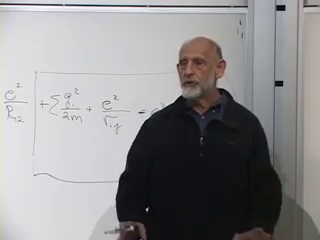
\includegraphics[width=0.72\textwidth]{lecture_01_figure_02.png}
\caption{Le Hamiltonien moléculaire reste au tableau lorsque le problème de l’état fondamental électronique est introduit. La forme saisie dans l’équation ~\eqref{eq:molecular-hamiltonian} rend compte des termes masqués sur cette image.}
\lectureframe{00:16:19}
\end{figure}

\begin{classroomqa}
\audiencequestion{Les impulsions nucléaires sont-elles simplement posées égales à zéro ?\lecturetimestamp{00:15:39}}
\lecturerresponse{Seulement de façon provisoire. Dans l’approximation dominante, on traite les noyaux comme s’ils étaient cloués sur place, car ils se déplacent beaucoup plus lentement que les électrons. Nous réintroduirons leurs impulsions lorsque nous résoudrons le problème nucléaire effectif ; cette approximation ne viole donc pas le principe d’incertitude.}
\end{classroomqa}

L’énergie de l’état fondamental électronique contribue désormais au potentiel ressenti par les noyaux :
\begin{equation}
V_{\mathrm{eff}}(R_1,R_2)
=\frac{e^2}{R_{12}}+E_{\mathrm{el}}(R_1,R_2).
\label{eq:molecular-effective-potential}
\end{equation}
L’invariance par rotation et par translation réduit, pour deux atomes isolés, ce potentiel à une fonction de leur séparation \(R_{12}\). À très courte distance, la répulsion coulombienne nucléaire domine. À très grande distance, l’interaction est faible. Entre ces deux limites, le nuage électronique peut créer une région attractive et un minimum. La fonction d’onde nucléaire se concentre alors près de ce minimum et décrit une molécule liée.

Remarquons l’ordre des opérations. Nous n’avons pas supposé une attraction empirique pour ensuite écarter les électrons. Nous avons d’abord résolu leur problème quantique dans le champ des noyaux fixes. Ce n’est qu’ensuite que nous avons éliminé leurs coordonnées explicites tout en conservant la valeur propre obtenue. La physique à courte distance subsiste dans la forme, la profondeur et la courbure de \(V_{\mathrm{eff}}\). La position de son minimum fixe la distance d’équilibre, sa courbure détermine les petites vibrations et son comportement asymptotique indique si un état lié existe. Une seule fonction effective transporte toute cette information électronique dans le problème plus lent.

Ainsi, un Hamiltonien complexe à plusieurs électrons est devenu un Hamiltonien nucléaire à deux corps doté d’un nouveau potentiel. Nous avons éliminé les degrés de liberté rapides tout en conservant leur effet complet à basse énergie. Le potentiel a été renormalisé. Ce raisonnement familier de Born--Oppenheimer n’est généralement pas présenté sous ce nom, mais il contient précisément l’idée dont nous avons besoin :
\begin{equation}
\begin{gathered}
\text{fast microscopic dynamics}\\
\Downarrow\\
\text{effective parameters for slow dynamics}
\end{gathered}
\end{equation}

\section{Unités naturelles et dimension d’un champ}

En théorie quantique des champs, les modes à éliminer peuvent être décrits de manière équivalente comme des modes à courte distance, à courte longueur d’onde, à haute fréquence ou à haute énergie. Avant de tracer des diagrammes, établissons le bilan dimensionnel.

En mécanique classique, la longueur, le temps et la masse sont des unités indépendantes. En physique des particules, nous posons
\begin{equation}
\hbar=c=1.
\end{equation}
L’énergie et la masse sont alors équivalentes par \(E=mc^2\), la longueur et le temps sont équivalents puisque \(c=1\), et \(\hbar=1\) fait de l’impulsion l’inverse d’une longueur. Il ne reste qu’une dimension :
\begin{equation}
[M]=[E]=[p]=L^{-1},
\qquad
[x]=[t]=L.
\label{eq:natural-units}
\end{equation}

Cela n’efface pas les dimensions. On choisit des facteurs de conversion tels qu’un temps puisse s’exprimer comme une longueur et une masse comme l’inverse d’une longueur. Une fois une unité spécifiée, toutes les autres en découlent. C’est pourquoi une coupure peut se décrire soit comme une courte distance \(\delta\), soit comme une haute énergie \(\Lambda=1/\delta\) : c’est la même échelle exprimée dans deux langages.

Considérons un champ scalaire réel \(\phi\), avec une densité lagrangienne normalisée de façon schématique :
\begin{equation}
\mathcal L=(\partial_\mu\phi)(\partial^\mu\phi)-V(\phi),
\qquad
S=\int d^4x\,\mathcal L.
\label{eq:scalar-action}
\end{equation}

\begin{figure}[htbp]
\centering
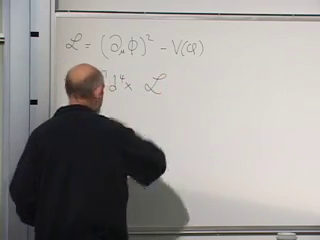
\includegraphics[width=0.78\textwidth]{lecture_01_figure_03.png}
\caption{La densité lagrangienne scalaire locale et son intégrale sur l’espace-temps, qui donne l’action.}
\lectureframe{00:26:08}
\end{figure}

La densité lagrangienne est locale : elle décrit un point de l’espace-temps. Les équations classiques du champ découlent de la stationnarité de l’action. En théorie quantique, cette même action intervient dans la phase de l’intégrale de chemin \(\exp(iS)\). Dans les deux approches, la dimension de \(S\) est déterminante. Si l’on rétablit \(\hbar\), la phase est \(\exp(iS/\hbar)\) ; après avoir posé \(\hbar=1\), \(S\) doit lui-même être sans dimension.

\begin{classroomqa}
\audiencequestion{L’action a-t-elle pour unité \(\hbar\) ?\lecturetimestamp{00:26:13}}
\lecturerresponse{Oui. Puisque \(\hbar\) a été posé égal à un, l’action est sans dimension dans ces unités. La mesure quadridimensionnelle est de dimension \(L^4\) ; la densité lagrangienne doit donc être de dimension \(L^{-4}\).}
\end{classroomqa}

Le terme cinétique fixe alors la dimension du champ :
\begin{align}
[S]&=1, & [\mathcal L]&=L^{-4},\\
[\partial_\mu]&=L^{-1}, &
[(\partial\phi)^2]&=L^{-2}[\phi]^2=L^{-4},\nonumber\\
&& [\phi]&=L^{-1}.
\label{eq:scalar-dimension}
\end{align}
Ce bref calcul déterminera le comportement ultraviolet de chaque diagramme qui suit.

Développons le potentiel sous la forme
\begin{equation}
V(\phi)=\frac{m^2}{2}\phi^2+g\phi^3+\lambda\phi^4+\cdots.
\label{eq:scalar-potential}
\end{equation}
Chaque terme doit être de dimension \(L^{-4}\). Puisque
\([\phi^n]=L^{-n}\),
\begin{equation}
[m^2]=L^{-2},
\qquad
[g]=L^{-1},
\qquad
[\lambda]=1.
\label{eq:coupling-dimensions}
\end{equation}
Le couplage quartique est sans dimension. De tels couplages sont particulièrement importants en renormalisation, car leur dépendance en échelle ne peut pas se déduire d’une simple puissance de la longueur.

\begin{classroomqa}
\audiencequestion{\(g\) a-t-il une dimension de masse ?\lecturetimestamp{00:29:52}}
\lecturerresponse{Oui. Le facteur \(\phi^3\) est de dimension \(L^{-3}\), tandis que la densité de potentiel doit être de dimension \(L^{-4}\). Par conséquent, \([g]=L^{-1}\), qui est une masse en unités naturelles.}
\end{classroomqa}

\section{Sommets et propagateur à courte distance}

Les règles de Feynman se construisent à partir des sommets et des propagateurs. Le terme \(g\phi^3\) donne un sommet à trois lignes, associé à un facteur proportionnel à \(g\) ; le terme \(\lambda\phi^4\) donne un sommet à quatre lignes, associé à un facteur proportionnel à \(\lambda\). Le terme quadratique donne une insertion locale à deux points. On peut la représenter par une particule qui arrive, est absorbée, puis réémise, avec un coefficient proportionnel à \(m^2/2\). Les normalisations numériques, les signes, les facteurs de \(i\) et les facteurs de symétrie sont délibérément omis : le cours cherche à dégager la dépendance en échelle, et non à calculer une section efficace.

Ces dessins ont une interprétation opérationnelle. Un sommet à trois points peut absorber deux quanta et en émettre un, ou représenter toute autre attribution de ses trois lignes liée par croisement. Un sommet à quatre points peut décrire deux particules entrantes et deux particules sortantes. La croix quadratique est bien un sommet à deux lignes, même si elle est normalement incorporée au propagateur libre. Nous l’indiquons parce que nous reconnaîtrons bientôt tout processus à deux points non résolu en le comparant à ce sommet.

Un propagateur relie deux points de l’espace-temps. Sa ligne ne signifie pas qu’une particule quantique a suivi une trajectoire classique rectiligne. Elle représente l’amplitude de créer une excitation du champ en \(x\) et de l’absorber ou de la détecter en \(y\) :
\begin{equation}
\Delta(x-y)=\langle0|\phi(y)\phi(x)|0\rangle.
\label{eq:position-propagator}
\end{equation}
Lisons l’expression de droite à gauche. L’action de \(\phi(x)\) sur le vide crée une composante à une particule en \(x\). L’action de \(\phi(y)\) sur le bra élimine la composante en \(y\). Leur élément de matrice dans le vide est l’amplitude de recouvrement entre la création au premier point et la détection au second. Les symboles \(x\) et \(y\) désignent des quadrivecteurs entiers, et non deux simples coordonnées cartésiennes.

Les états sont sans dimension physique, tandis que chaque champ apporte \(L^{-1}\). Par conséquent,
\begin{equation}
[\Delta]=L^{-2}.
\end{equation}
Pour un champ sans masse, il n’existe pas d’échelle de longueur intrinsèque ; l’analyse dimensionnelle impose donc le comportement à courte distance
\begin{equation}
\Delta(x-y)\sim\frac{1}{(x-y)^2}.
\label{eq:massless-propagator}
\end{equation}
Le dénominateur est la séparation au carré invariante de Lorentz, avec la prescription usuelle au voisinage de ses singularités.\editorialnote{Pour le décompte des puissances, il est commode de faire une rotation de Wick vers une séparation euclidienne, dont le module est sans ambiguïté proportionnel à \(1/|x-y|^2\). Cela ne modifie pas les puissances ultraviolettes utilisées ci-dessous.}

Lorsque \(y\) tend vers \(x\), le propagateur diverge. Cette singularité de propagation sur une séparation qui tend vers zéro est à l’origine des divergences ultraviolettes des diagrammes plus élaborés.

\section{Renormalisation de la masse d’un scalaire}

Pour un champ scalaire, le paramètre dynamique est \(m^2\), comme le suggère déjà la relation de dispersion relativiste :
\begin{equation}
E=\sqrt{\mathbf p^2+m^2}.
\end{equation}
Soit \(\delta\) la plus petite distance que notre description effective permet de résoudre. Nous ne distinguerons pas les processus dont les sommets sont séparés par une distance inférieure à \(\delta\). Tout processus non résolu de ce type, avec un scalaire entrant et un scalaire sortant, a la même structure observable à deux points qu’une insertion de masse ; il doit donc contribuer à la masse effective.

Considérons un accélérateur comme un microscope. Si sa résolution la plus fine est \(\delta\), une absorption en un point suivie d’une émission à une distance bien inférieure à \(\delta\) ne peut être distinguée d’un événement véritablement local. Nous floutons délibérément le sommet à cette échelle. La renormalisation est la règle qui transfère tous ces processus possibles, situés sous le seuil de résolution, dans le coefficient de l’opérateur local correspondant.

\subsection{Première correction quartique}

Commençons par un unique sommet \(\phi^4\). Deux lignes correspondent à la particule externe ; les deux autres se rejoignent pour former une petite boucle, émise puis réabsorbée presque au même point. En étalant le propagateur au point coïncident sur la distance de coupure, on obtient
\begin{equation}
\Delta(0)\ \longrightarrow\ \Delta(\delta)\sim\frac{1}{\delta^2},
\end{equation}
d’où
\begin{equation}
\delta m^2_{(1)}\sim\frac{\lambda}{\delta^2}.
\label{eq:one-loop-scalar-mass}
\end{equation}
Si \(m_0^2\) désigne le paramètre d’entrée, ou paramètre nu, le coefficient à deux points mesuré à basse résolution prend schématiquement la forme
\begin{equation}
\frac{m_{\mathrm{eff}}^2}{2}
\sim
\frac{m_0^2}{2}
+c_1\frac{\lambda}{\delta^2},
\label{eq:first-renormalized-mass}
\end{equation}
où \(c_1\) regroupe les facteurs numériques et les conventions omis. La masse mesurée en laboratoire dans des expériences qui ne résolvent pas les distances inférieures à \(\delta\) est cette quantité renormalisée, et non \(m_0\) à elle seule.

Il existe donc deux façons indiscernables de produire l’événement observé à deux points. Le sommet quadratique initial peut absorber puis réémettre la particule, ou bien l’interaction quartique peut le faire en émettant puis en réabsorbant brièvement un scalaire virtuel. En mécanique quantique, les amplitudes s’additionnent. Dès que la boucle se trouve sous le seuil de résolution, son histoire distincte disparaît de la description effective, mais sa contribution au coefficient mesuré demeure.

\subsection{Correction quartique suivante}

Relions maintenant deux sommets quartiques de sorte qu’une particule externe entre en \(x\), qu’une autre en sorte en \(x+\Delta\) et que trois propagateurs internes relient les sommets. On a deux puissances de \(\lambda\), tandis que les propagateurs apportent \(\Delta^{-6}\). Les amplitudes quantiques doivent être sommées sur tous les points non résolus d’où la particule sortante peut émerger ; on intègre donc sur le quadrivecteur relatif :
\begin{equation}
\delta m^2_{(2)}
\sim
\lambda^2
\int_{|\Delta|\gtrsim\delta}
d^4\Delta\,\frac{1}{|\Delta|^6}.
\label{eq:two-loop-power-count}
\end{equation}

\begin{classroomqa}
\audiencequestion{La petite marque au sommet signifie-t-elle qu’il n’y a que trois particules à cet endroit ?\lecturetimestamp{00:46:35}}
\lecturerresponse{Non. Nous utilisons toujours l’interaction quartique. Quatre lignes se rejoignent à chaque sommet ; dans ce diagramme à deux points, une ligne est externe et trois relient les deux sommets. Le second sommet a également quatre lignes incidentes.}
\end{classroomqa}

La mesure apporte quatre puissances de longueur et les trois propagateurs en apportent moins six. Puisque la coupure ultraviolette est la seule échelle de cette estimation,
\begin{equation}
\int_{|\Delta|\gtrsim\delta}
\frac{d^4\Delta}{|\Delta|^6}
\sim\frac{1}{\delta^2},
\qquad
\delta m^2_{(2)}
\sim\frac{\lambda^2}{\delta^2}.
\label{eq:two-loop-scalar-mass}
\end{equation}
Ici, \(\Delta^\mu\) est une variable d’intégration à quatre composantes ; on intègre sur sa composante temporelle et ses trois composantes spatiales. Le \(\delta\) minuscule désigne la coupure fixe. Le cours emploie d’abord le même nom oral pour les deux, puis rectifie la notation.

On retrouve le même résultat en exprimant radialement la mesure quadridimensionnelle. À une constante angulaire près,
\begin{equation}
\int_{\delta}\frac{d^4\Delta}{|\Delta|^6}
\sim
\int_{\delta}\frac{R^3\,dR}{R^6}
=\int_{\delta}\frac{dR}{R^3}
\sim\frac{1}{\delta^2}.
\end{equation}
C’est pourquoi la limite supérieure à grande distance n’a pas d’importance pour l’estimation ultraviolette : l’intégrale est dominée par son extrémité inférieure.

Les diagrammes d’ordre supérieur reproduisent le même schéma. Un diagramme avec davantage de sommets quartiques ajoute une puissance supérieure de \(\lambda\), mais l’analyse dimensionnelle autorise toujours une contribution quadratiquement divergente à la masse :
\begin{equation}
\begin{aligned}
m_{\mathrm{eff}}^2
={}&m_0^2
+\frac{1}{\delta^2}
\left(c_1\lambda+c_2\lambda^2+c_3\lambda^3+\cdots\right)\\
&+\text{weaker terms}.
\end{aligned}
\label{eq:scalar-mass-series}
\end{equation}

\subsection{Interaction cubique et logarithme}

Deux sommets cubiques donnent deux propagateurs entre des points proches. Leur contribution est proportionnelle à
\begin{equation}
\delta m_g^2
\sim
g^2\int_{|\Delta|\gtrsim\delta}
\frac{d^4\Delta}{|\Delta|^4}.
\label{eq:cubic-loop}
\end{equation}
Cette fois, la mesure et le dénominateur portent le même nombre de puissances. La dépendance restante est logarithmique plutôt qu’une puissance :
\begin{equation}
\delta m_g^2
\sim
c_g g^2\log\!\left(\frac{1}{\mu\delta}\right).
\label{eq:cubic-log}
\end{equation}
L’échelle de référence \(\mu\) rend le logarithme sans dimension. C’est la version entièrement dimensionnée de l’expression schématique \(g^2\log\delta\) du cours. Un logarithme varie beaucoup plus lentement que n’importe quelle puissance inverse ; ainsi, \(1/\delta^2\) domine lorsque la coupure correspond à une distance de plus en plus courte.

La forme radiale rend, là encore, la distinction évidente :
\begin{equation}
\int_{\delta}^{R_{\mathrm{IR}}}
\frac{d^4\Delta}{|\Delta|^4}
\sim
\int_{\delta}^{R_{\mathrm{IR}}}\frac{R^3\,dR}{R^4}
=\log\!\left(\frac{R_{\mathrm{IR}}}{\delta}\right).
\end{equation}
Quand les puissances de la mesure et du dénominateur sont égales, on obtient un logarithme. Si le dénominateur comporte davantage de puissances, on obtient une puissance inverse de la coupure. Le cours ne nous demande pas d’évaluer les facteurs angulaires ; il nous apprend à reconnaître immédiatement la réponse ultraviolette.

\begin{classroomqa}
\audiencequestion{Quelle base utilise-t-on pour le logarithme ?\lecturetimestamp{00:57:42}}
\lecturerresponse{On utilise le logarithme népérien. Un changement de base ne fait que le multiplier par une constante numérique, laquelle est absorbée dans le coefficient dont les facteurs de \(2\), de \(\pi\) et de symétrie n’ont pas été calculés ici.}
\end{classroomqa}

\begin{classroomqa}
\audiencequestion{Comment peut-on prendre le logarithme d’une longueur, et d’où viennent les unités de la correction de masse ?\lecturetimestamp{00:58:32}}
\lecturerresponse{Un logarithme compare toujours deux échelles ; il s’agit donc, rigoureusement, du logarithme d’un rapport sans dimension tel que \(1/(\mu\delta)\). Le couplage \(g\) a une puissance de masse ; \(g^2\) possède donc déjà exactement la dimension d’une masse au carré requise pour la correction.}
\end{classroomqa}

\begin{classroomqa}Un diagramme de Feynman donne une amplitude. Le carré de son module est-il une probabilité ?\audiencequestion{
\lecturetimestamp{00:59:41}}\lecturerresponse{Oui, lorsque l’amplitude intervient dans le calcul d’une transition physique avec les facteurs d’états et d’espace des phases requis. Ici, son rôle immédiat est différent : l’amplitude non résolue d’un processus à deux points a la même forme locale que le terme de masse et déplace donc le paramètre de masse effective.}
\end{classroomqa}

\section{Tous les paramètres deviennent effectifs}

La famille infinie de diagrammes de masse ne disparaît pas simplement parce que \(\lambda\) est petit. La théorie des perturbations les ordonne selon les puissances du couplage ; les termes successifs peuvent donc être de plus en plus petits, mais ils restent en nombre infini. L’élimination des courtes distances renormalise également les interactions elles-mêmes.

\begin{classroomqa}
\audiencequestion{Même pour la renormalisation de la masse, n’y a-t-il pas une infinité de diagrammes ?\lecturetimestamp{01:00:35}}
\lecturerresponse{Si. Si \(\lambda\) est suffisamment petit, la série perturbative peut être utile, car les puissances supérieures sont successivement supprimées. Néanmoins, le paramètre renormalisé est défini par la série entière, et non par le seul premier diagramme.}
\end{classroomqa}

Sur le plan opérationnel, une interaction locale \(\lambda\phi^4\) est une amplitude à deux particules entrantes et deux particules sortantes. Si un processus à quatre points plus complexe se déroule entièrement dans une région non résolue, il est indiscernable, à basse résolution, du sommet local initial. Ces diagrammes sont donc regroupés dans un \(\lambda\) effectif. En quatre dimensions, leur dépendance dominante en échelle est généralement logarithmique dans la théorie \(\phi^4\). Le cours ne calcule pas cette fonction bêta ; il se sert de cet exemple pour énoncer le principe général :
\begin{equation}
\begin{gathered}
\text{parameters measured at low energy}\\
\ne\\
\text{parameters entered at the microscopic cutoff}
\end{gathered}
\end{equation}

L’exemple à quatre points est important, car il écarte un possible malentendu. La renormalisation n’est pas une réparation spéciale appliquée uniquement à une divergence de masse. Tout opérateur autorisé dans le lagrangien peut être reproduit par des diagrammes non résolus ayant les mêmes lignes externes et les mêmes symétries. Un processus à deux points renormalise un coefficient quadratique, un processus à quatre points renormalise un coefficient quartique, et les processus du vide au vide renormalisent le terme constant. Le lagrangien à basse énergie est le registre concis où sont consignés tous ces processus à courte distance.

\begin{classroomqa}
\audiencequestion{Puisque \(\Delta\) a pour unité une longueur, prendre son logarithme n’est-il pas dimensionnellement étrange ? Et le tableau a-t-il interverti delta majuscule et delta minuscule ?\lecturetimestamp{01:01:34}}
\lecturerresponse{Le logarithme désigne en réalité le rapport à une autre échelle ; il est donc sans dimension. Oui, la notation a été brièvement intervertie : \(\Delta^\mu\) est la variable d’intégration, tandis que \(\delta\) est la coupure de distance inférieure qui subsiste dans le résultat.}
\end{classroomqa}

C’est l’équivalent, en théorie des champs, du cas de la molécule. Nous avons résolu le mouvement des électrons rapides, invisibles, puis intégré leur résultat dans un potentiel. Ici, nous faisons la somme des processus invisibles à courte distance et intégrons leur résultat dans les masses, les couplages et tous les autres coefficients locaux autorisés. Tous les paramètres sont décalés.

\begin{classroomqa}
\audiencequestion{Pourriez-vous répéter si la quantité mesurée inclut les échelles plus petites que celles que l’expérience peut voir ?\lecturetimestamp{01:05:13}}
\lecturerresponse{Oui. Les fluctuations individuelles ne sont pas résolues, mais leur effet cumulé est présent. Tous les diagrammes qui font intervenir des échelles plus courtes sont regroupés dans un unique coefficient effectif, que l’expérience à basse énergie interprète par exemple comme la masse au carré physique.}
\end{classroomqa}

\begin{classroomqa}
\audiencequestion{Le terme d’entrée \(m_0^2\) doit-il alors annuler les autres contributions ?\lecturetimestamp{01:06:00}}
\lecturerresponse{Si la masse scalaire mesurée est bien plus petite que les contributions ultraviolettes prises individuellement, oui. Cette annulation nécessaire est le problème du réglage fin que nous allons maintenant aborder.}
\end{classroomqa}

\section{Le problème de la hiérarchie du Higgs}

Imaginons que la coupure soit la longueur de Planck, de sorte que la théorie effective des champs doit résumer les fluctuations depuis les échelles de laboratoire jusqu’à l’échelle où la gravité quantique doit intervenir. En unités de physique des particules,
\begin{equation}
\delta\sim M_{\mathrm{Pl}}^{-1}\sim10^{-19}\,\mathrm{GeV}^{-1},
\qquad
\frac{1}{\delta^2}\sim10^{38}\,\mathrm{GeV}^2.
\label{eq:planck-cutoff}
\end{equation}
Le choix précis entre l’échelle de Planck réduite et non réduite ne change rien à l’énormité de l’écart.

La hiérarchie des distances est tout aussi frappante. La longueur de Planck est environ dix-neuf ordres de grandeur inférieure au rayon du proton, et environ seize ou dix-sept ordres de grandeur inférieure aux distances directement sondées par les accélérateurs évoqués ici. Le fait d’élever cet écart au carré conduit à l’annulation d’environ trente-quatre ordres de grandeur dans un paramètre de masse scalaire au carré.

Pour le champ de Higgs, qui est un scalaire, l’échelle faible recherchée est de l’ordre de quelques centaines de GeV, et non de \(10^{19}\) GeV. Pourtant, les termes de l’équation~\eqref{eq:scalar-mass-series} peuvent naturellement être de l’ordre de l’échelle de Planck.
Leurs signes n’ont pas été suivis : certains peuvent être positifs, d’autres négatifs, et la masse au carré nue peut elle aussi avoir l’un ou l’autre signe. Mais, pour laisser un résidu à l’échelle électrofaible, ces contributions énormes doivent s’annuler à environ trente-quatre chiffres après la virgule. Susskind commence par dire dix-sept chiffres, puis se corrige, car la comparaison porte sur des masses au carré. C’est le rapport au carré qui mesure ce réglage dans ce cas.

\begin{classroomqa}
\audiencequestion{\(\lambda\) est-il inférieur ou supérieur à un ?\lecturetimestamp{01:09:50}}
\lecturerresponse{On suppose qu’il est légèrement inférieur à un. La théorie des perturbations deviendrait inextricable si les puissances successives augmentaient, et une théorie purement scalaire ne peut pas non plus être extrapolée de manière cohérente avec un couplage quartique arbitrairement grand. Mais \(\lambda\) est loin d’être aussi petit que \(10^{-38}\) ; pour se repérer, le cours retient une valeur de l’ordre du pour cent.}
\end{classroomqa}

\begin{classroomqa}
\audiencequestion{Même si \(\lambda<1\), ne reste-t-il pas beaucoup de termes importants, puisque chacun comporte le grand facteur de coupure ?\lecturetimestamp{01:10:43}}
\lecturerresponse{Oui. Les puissances élevées finissent par supprimer la série, mais un grand nombre de termes peuvent contribuer avant que cela ne se produise. Ces termes et le terme nu devraient tous se compenser de façon à ne laisser que la valeur physique extraordinairement petite.}
\end{classroomqa}

Rappelons pourquoi l’on sait que le paramètre de masse du boson de Higgs est à l’échelle électrofaible. Avec les conventions du cours, écrivons le potentiel de brisure de symétrie sous la forme
\begin{equation}
V(\phi)=-\frac{\mu^2}{2}\phi^2+\frac{\lambda}{4}\phi^4.
\label{eq:higgs-potential}
\end{equation}
Le coefficient quadratique négatif rend l’origine instable, tandis que le terme quartique positif stabilise le potentiel. En dérivant,
\begin{equation}
\frac{dV}{d\phi}=-\mu^2\phi+\lambda\phi^3
=\phi(-\mu^2+\lambda\phi^2),
\end{equation}
on obtient le minimum non nul
\begin{equation}
\phi_{\min}^2=f^2=\frac{\mu^2}{\lambda}.
\label{eq:higgs-minimum}
\end{equation}
Le tableau écrit le terme quartique de façon schématique sous la forme \(\lambda\phi^4\), mais cite l’équation ~\eqref{eq:higgs-minimum} ; l’insertion du facteur conventionnel \(1/4\) rend ces deux lignes cohérentes sans modifier l’argument.

Le signe de \(-\mu^2\) est important, mais ne résout pas le problème de naturalité. C’est la courbure négative à l’origine qui entraîne la brisure spontanée de symétrie. La renormalisation modifie cette courbure par de grandes contributions positives et négatives. Pour obtenir le vide brisé observé, leur somme doit non seulement être petite, mais prendre la valeur négative précise qui place le minimum à l’échelle électrofaible.

Les masses des bosons \(W\) et \(Z\) déterminent \(f\) comme étant de l’ordre de \(200\,\mathrm{GeV}\) selon la normalisation approximative utilisée dans le cours. Si \(\lambda\) n’est ni énorme ni extraordinairement petit, \(\mu\) doit être du même ordre général. Le coefficient observé à l’échelle électrofaible est donc le résidu de contributions qui peuvent chacune être supérieures de plusieurs dizaines d’ordres de grandeur.

On appelle cela le problème du réglage fin du boson de Higgs, le problème de la hiérarchie ou le problème de la hiérarchie de jauge. La hiérarchie est le rapport immense entre l’échelle électrofaible ordinaire et une éventuelle échelle d’unification ou de Planck. Un petit nombre n’est pas en soi paradoxal. Ce qui est troublant ici, c’est qu’un petit nombre résulte de contributions importantes, apparemment sans rapport, qui doivent s’annuler avec une extrême précision. Le problème a été reconnu à la fin des années 1970 et au début des années 1980, et la recherche d’un mécanisme à l’origine de cette annulation motive la supersymétrie ainsi que plusieurs idées concurrentes.

La série perturbative infinie aiguise le problème au lieu de le résoudre. Une valeur de \(\lambda\) de l’ordre du pour cent rend suffisamment petites les puissances assez élevées, mais de nombreux termes peuvent apparaître avant que cette suppression ne l’emporte. Il ne suffit pas qu’une boucle annule fortuitement la masse nue. L’échelle électrofaible effective doit rester stable après inclusion du reste des processus à courte distance. Une relation structurelle entre les termes fournirait une explication ; une annulation chiffre par chiffre entre des contributions sans rapport ne constitue qu’un réglage fin.

\section{Pourquoi la masse d’un fermion se comporte mieux}

Les autres particules du Modèle standard ne nécessitent pas de réglages fins indépendants du même type. Pour un fermion de Dirac, le terme de masse est
\begin{equation}
\mathcal L_m=-m\bar\psi\psi
=-m\left(\bar\psi_L\psi_R+\bar\psi_R\psi_L\right).
\label{eq:fermion-mass}
\end{equation}
Il contient la masse, et non son carré, et couple les chiralités gauche et droite. Une insertion locale de masse transforme donc \(L\) en \(R\), ou \(R\) en \(L\).

\begin{figure}[htbp]\centering
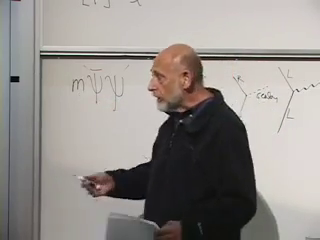
\includegraphics[width=0.76\textwidth]{lecture_01_figure_04.png}\caption{Le terme de masse du fermion et les schémas tracés au tableau illustrant les changements de chiralité. Les diagrammes sont reconstitués algébriquement ci-dessous, car une partie du travail à la craie est masquée.}\lectureframe{01:23:36}\end{figure}

Dans le cours oral, il est souvent question de caractère droitier ou de l’hélicité. La protection exacte s’énonce le plus clairement en termes de chiralité. Pour une particule ultrarelativiste, l’image fondée sur l’hélicité donne l’intuition recherchée, mais la chiralité est la grandeur portée par les champs gauches et droits dans l’équation ~\eqref{eq:fermion-mass}.

Les interactions de jauge préservent la chiralité :
\begin{equation}
L\xrightarrow{\ \gamma\ }L,
\qquad
R\xrightarrow{\ \gamma\ }R.
\label{eq:gauge-preserves-chirality}
\end{equation}
Une interaction de Yukawa avec un scalaire relie des chiralités opposées :
\begin{equation}
L\xleftrightarrow{\ \phi\ }R.
\label{eq:scalar-flips-chirality}
\end{equation}
Supposons d’abord que l’électron soit initialement dans l’état \(m_0=0\). L’émission puis la réabsorption d’un nombre quelconque de photons ne peuvent pas produire de masse, car chaque vertex de jauge préserve la chiralité. Une suite d’interactions qui commence à gauche reste à gauche. L’électrodynamique quantique pure permet donc de manière cohérente un électron sans masse : son auto-énergie électromagnétique ne peut pas engendrer une masse additive à partir de zéro.

Dans le schéma de lignes, partons d’un électron de chiralité gauche. Au premier vertex photonique, sa chiralité est toujours gauche ; après la propagation et la réabsorption du photon, elle est encore gauche. Répéter cette construction ne fait qu’insérer davantage de vertex qui préservent la chiralité. La fonction à deux points externe peut être renormalisée, mais elle ne peut pas acquérir la structure gauche-droite qui définit une masse.

L’émission d’un scalaire pourrait-elle y parvenir ? Un vertex scalaire transforme \(L\) en \(R\), mais le scalaire émis doit être réabsorbé. Un graphe d’auto-énergie à deux points contient donc un nombre pair de vertex scalaires. Le second changement de chiralité inverse le premier, si bien que le graphe complet préserve à nouveau la chiralité externe. Quelle que soit la complexité du graphe interne, l’appariement des vertex par émission et réabsorption empêche l’apparition d’un terme de \(L\) à \(R\) additif lorsque la masse initiale est nulle.

Il s’agit d’un argument de parité sur le nombre de changements de chiralité. Un vertex scalaire change la chiralité une fois ; la fermeture de chaque ligne scalaire interne exige une seconde extrémité, et donc un second changement de chiralité. Quatre vertex scalaires entraînent quatre changements, et ainsi de suite. Un nombre pair ramène le fermion à sa chiralité initiale. Cette conclusion ne se limite pas à la boucle la plus simple dessinée au tableau.

Une correction de masse non nulle n’est possible que si le diagramme contient déjà une insertion de masse. Par exemple, l’émission et la réabsorption d’un photon peuvent encadrer une insertion de \(m_0\bar\psi\psi\). Les vertex de jauge apportent deux puissances de la charge électrique, mais le seul changement de chiralité apporte la masse initiale :
\begin{equation}
\begin{aligned}
m_e
&=m_0+c_1e^2m_0+c_2e^4m_0+\cdots\\
&=m_0\left(1+c_1e^2+c_2e^4+\cdots\right).
\end{aligned}
\label{eq:multiplicative-fermion-mass}
\end{equation}
Si \(m_0=0\), le résultat reste nul. Si \(m_0\) est petit, chaque correction est proportionnelle à ce petit nombre. On peut toujours se demander pourquoi l’électron est léger par rapport à une échelle fondamentale, mais on n’a plus à soustraire de grandes quantités sans rapport pour l’obtenir. En ce sens, une faible masse de fermion est techniquement naturelle.

L’insertion de masse explicite la séquence autorisée. Partons de \(L\). L’émission d’un photon préserve \(L\) ; l’insertion \(m_0\) transforme \(L\) en \(R\) ; la réabsorption du photon préserve \(R\). Le diagramme possède maintenant la chiralité externe d’un terme de masse, mais sa valeur comporte nécessairement le facteur \(m_0\). C’est là le contraste crucial avec l’équation ~\eqref{eq:one-loop-scalar-mass}, dont la correction scalaire reste non nulle même lorsque la masse scalaire initiale est fixée à zéro.

Les bosons de jauge bénéficient d’une protection analogue : la symétrie de jauge interdit un terme de masse indépendant, de sorte qu’un boson de jauge initialement sans masse le reste à tous les ordres perturbatifs. Dans le Modèle standard, les masses des fermions et des bosons de jauge faibles apparaissent en réponse à la valeur moyenne dans le vide du champ de Higgs. Si l’échelle du Higgs est maîtrisée, les autres masses légères n’exigent pas de reproduire séparément le même réglage fin catastrophique.

Cela précise la question à laquelle la supersymétrie entend répondre : une théorie peut-elle empêcher le scalaire de Higgs de recevoir une correction de masse additive énorme ? La réponse est oui dans des cadres supersymétriques appropriés, parce que les contributions bosoniques et fermioniques sont liées plutôt qu’indépendantes. Le mécanisme détaillé sera abordé dans le cours suivant.

\section{L’autre réglage fin : l’énergie du vide}

Il existe un problème de renormalisation encore plus grave, mais il ne devient observable que lorsque l’on inclut la gravité. En physique non gravitationnelle, ajouter une constante à toutes les énergies ne modifie aucune expérience. La masse de l’électron, par exemple, n’est pas une énergie absolue ; c’est l’énergie supplémentaire nécessaire pour ajouter un électron au vide :
\begin{equation}
m_e=E(\text{vacuum}+\text{one electron})-E(\text{vacuum})
\end{equation}
dans le référentiel de repos de l’électron. Si le vide et tous les états excités sont décalés de la même façon, leurs différences restent inchangées.

Les diagrammes du vide au vide modifient néanmoins l’énergie du vide. Dans la théorie \(\lambda\phi^4\), réunissons les quatre pattes d’un vertex quartique en deux boucles courtes. Chaque propagateur pris au même point fournit \(1/\delta^2\), donc
\begin{equation}
\delta\rho_{\mathrm{vac}}
\sim
c_{\mathrm{vac}}\frac{\lambda}{\delta^4}.
\label{eq:vacuum-energy-divergence}
\end{equation}
Les diagrammes du vide plus complexes comportent d’autres facteurs de couplage et coefficients, mais l’analyse dimensionnelle donne généralement la même dépendance quartique à la coupure pour une densité d’énergie.

L’absence de lignes externes identifie précisément la correction. Les graphes à deux points comparent un état à une particule au vide et modifient une masse ; les graphes à quatre points modifient la diffusion ; un graphe sans particules entrantes ni sortantes modifie l’amplitude du vide au vide elle-même. Un vertex quartique fournit \(\lambda\), et ses deux boucles courtes fournissent chacune \(\delta^{-2}\). L’analyse dimensionnelle impose alors l’échelle de densité d’énergie \(\delta^{-4}\).

Sans gravité, on peut choisir le zéro de l’énergie et se demander à qui cela importe. La relativité générale supprime cette liberté : le tenseur énergie-impulsion est une source de la courbure de l’espace-temps, si bien qu’une énergie uniforme du vide fait graviter l’espace vide. Elle apparaît sous la forme d’une constante cosmologique et est reliée, du point de vue observationnel, à l’énergie noire. Une énergie du vide mesurée comme infime doit alors subsister malgré des contributions de la forme \(\delta^{-4}\).

Voilà pourquoi la question change lorsqu’on introduit la gravité. En mécanique quantique ordinaire, décaler tous les niveaux d’une même constante ne modifie aucune fréquence de transition. En gravité, cette constante n’est pas inerte : le tenseur de contrainte du vide est proportionnel à la métrique et courbe l’espace-temps. Ce qui était un zéro arbitraire de l’énergie devient une source dans l’équation d’Einstein.

Il existe donc au moins deux problèmes de naturalité extrêmes. Le cours évoque environ 123 décimales de réglage fin pour l’énergie du vide et environ 30--35 pour la masse du Higgs. Les nombres exacts dépendent de l’échelle ultraviolette et des conventions, mais le contraste ne fait aucun doute. La supersymétrie est une réponse possible au problème du Higgs abordé ici ; une fois brisée, elle n’explique pas à elle seule la constante cosmologique observée.\editorialnote{C’est aussi pourquoi une annulation exacte boson--fermion ne constitue pas une solution phénoménologique à l’énergie du vide observée : la supersymétrie doit être brisée dans notre monde.}

\section{Questions de fin de cours}

\begin{classroomqa}
\audiencequestion{La correction au Higgs dépend de la coupure \(\delta\), mais celle-ci semble arbitraire. Pourrait-elle correspondre à la longueur de Planck, à dix fois la longueur de Planck ou à autre chose ? Cela rend-il le réglage fin arbitraire ?\lecturetimestamp{01:33:50}}
\lecturerresponse{La contribution numérique dépend de l’échelle la plus courte jusqu’à laquelle on peut faire confiance à la théorie effective. Cette dépendance relève du bilan physique, elle ne permet pas d’échapper au problème. Les modes jusqu’à toute échelle où le Modèle standard reste valable sont des modes dont il faut inclure les effets. Choisissons \(\delta\) à la distance où l’on s’attend à ce qu’une nouvelle physique apparaisse---peut-être l’échelle de Planck, peut-être une échelle d’unification proche de \(10^{16}\,\mathrm{GeV}\). La contribution accumulée jusqu’à cette échelle constitue déjà une borne inférieure du problème. Prolonger la même théorie jusqu’à des distances encore plus courtes ne fait qu’accroître la dépendance quadratique. Nous devons expliquer ce qui annule la contribution provenant de chaque échelle entre le laboratoire et cette limite ultraviolette.}
\end{classroomqa}

\begin{classroomqa}
\audiencequestion{Qu’est-ce qui définit une particule scalaire, et quel en est un exemple ?\lecturetimestamp{01:37:26}}
\lecturerresponse{Le Higgs est l’exemple visé. Un scalaire ne se transforme pas en différentes composantes sous une rotation spatiale ; de manière équivalente, ses quanta ont un spin nul. Le photon est décrit par un champ vectoriel, et le champ gravitationnel par un tenseur. À l’époque de cette conférence 2010, aucune particule élémentaire de spin nul n’avait encore été détectée.\editorialnote{Le boson de Higgs a été découvert au CERN en 2012 et ses propriétés mesurées sont compatibles avec un spin nul.}}
\end{classroomqa}

\begin{classroomqa}
\audiencequestion{La particule \(Z\) est-elle aussi un boson de jauge ?\lecturetimestamp{01:38:31}}
\lecturerresponse{Oui. Les \(Z\), \(W^+\) et \(W^-\) sont des bosons de jauge de spin un, tout comme le photon. Leurs équations de champ et leurs interactions sont des généralisations non abéliennes ou électrofaibles de la description de jauge de type Maxwell.}
\end{classroomqa}

\begin{classroomqa}
\audiencequestion{Pourquoi la contribution de l’état fondamental bosonique ne s’annule-t-elle pas avec la contribution fermionique dans l’énergie du vide ?\lecturetimestamp{01:39:10}}
\lecturerresponse{Les boucles de fermions et les boucles bosoniques correspondantes peuvent effectivement contribuer avec des signes opposés. L’annulation n’est toutefois pas automatique : les masses, les multiplicités et les couplages des particules doivent correspondre. Même un faible désaccord laisse un résidu important dépendant de la coupure, et les familles infinies de diagrammes doivent correspondre ordre par ordre. La supersymétrie exacte impose précisément de telles relations boson--fermion. Le contenu générique en particules d’une théorie non supersymétrique ne les impose pas, et une supersymétrie brisée laisse subsister un problème d’énergie du vide.}
\end{classroomqa}

\section{Mise en perspective}

Le parcours du cours suit un enchaînement délibéré. Un calcul moléculaire montre d’abord que l’élimination des variables rapides n’est ni une négligence ni un tour de magie : leur énergie d’état fondamental devient un potentiel pour les variables lentes. La théorie quantique des champs répète cette opération à différentes longueurs d’onde. L’analyse dimensionnelle révèle ensuite quels paramètres effectifs sont sensibles à la coupure. Les masses scalaires reçoivent des termes additifs proportionnels à \(\delta^{-2}\) ; l’échelle du Higgs, lorsqu’elle est faible, semble donc d’une fragilité contre nature. Les masses des fermions sont renormalisées multiplicativement, car la chiralité protège la limite de masse nulle ; la symétrie de jauge protège de même les bosons de jauge sans masse. L’énergie du vide est encore plus sensible et varie comme \(\delta^{-4}\) ; la gravité rend sa valeur absolue observable.

La supersymétrie intervient dans le cours précisément à ce stade, non comme un ornement mathématique, mais comme une tentative de faire se comporter le secteur scalaire davantage comme les secteurs protégés. L’étape suivante consiste à comprendre quelle symétrie peut relier les bosons et les fermions assez étroitement pour organiser ces annulations.

\chapter{Signes des fermions et annulations supersymétriques}

\lectureoverview{La supersymétrie relie bosons et fermions, mais on comprend mieux pourquoi on souhaite une telle relation avant d’en écrire l’algèbre. Nous partons de la topologie des rotations, rendons observable par interférence le signe de la fonction d’onde d’un fermion, déduisons le signe négatif d’une boucle fermionique fermée de l’antisymétrie par échange, puis utilisons les signes opposés des boucles bosoniques et fermioniques pour motiver l’annulation de l’énergie du vide et de l’auto-énergie des scalaires. Dans la seconde moitié, nous nous demandons dans quelle mesure la supersymétrie peut être brisée, comment détecter les partenaires supersymétriques et pourquoi une supersymétrie exacte ferait disparaître la structure ordinaire des couches atomiques.}

\section{Avant la supersymétrie : une particularité des rotations}

La supersymétrie est une symétrie entre fermions et bosons. Toutefois, avant d’essayer de la construire, il est utile de rappeler à quel point ces deux types de particules réagissent différemment aux rotations. Cette question commence par un fait topologique facile à démontrer, mais étonnamment difficile à oublier une fois qu’on l’a vu.

Tenez une main, paume tournée vers le haut, et faites pivoter le poignet de \(2\pi\). La main retrouve son orientation initiale, mais le bras, à l’évidence, n’est pas revenu à une configuration équivalente : il est vrillé. Continuez sur encore \(2\pi\), en faisant bouger le bras au besoin, et la torsion peut être défaite. Ainsi, une rotation de \(2\pi\) ne peut pas être déformée continûment en l’absence de rotation si l’on maintient l’environnement fixe, tandis qu’une rotation de \(4\pi\) le peut. La démonstration avec la main est une preuve par un geste de la main, au sens le plus littéral du terme.

On peut établir le même point sans s’appuyer sur l’anatomie. Placez une balle dans une boîte fixe et reliez-la aux parois par autant de ficelles flexibles et extensibles, mais incassables, que vous le souhaitez. Faites tourner la balle d’un tour de \(2\pi\). Les ficelles s’emmêlent, et aucun mouvement des ficelles seul ne permet de retrouver la configuration initiale. Faites tourner la balle d’un angle total \(4\pi\), et les ficelles peuvent être déplacées autour d’elle jusqu’à ce que l’entrelacs disparaisse. Les parois représentent l’infini spatial : la comparaison n’a de sens que parce que la frontière ne tourne pas avec la balle.

\begin{classroomqa}
\audiencequestion{Peut-on défaire l’entrelacs en faisant tourner la boîte ? \lecturetimestamp{00:02:53}}
\lecturerresponse{Cela change le problème. La boîte représente l’infini spatial et reste fixe. Nous comparons la rotation de l’objet par rapport à son environnement, et non une rotation commune de l’objet et de son environnement.}
\end{classroomqa}

\begin{classroomqa}
\audiencequestion{Pourquoi ne pas simplement faire tourner la balle d’un autre \(2\pi\)? \lecturetimestamp{00:03:20}}
\lecturerresponse{C’est précisément ce qui distingue les deux cas. Sans faire tourner davantage la balle, l’entrelacs laissé par un tour de \(2\pi\) ne peut pas être défait. Après un second tour, soit un total de \(4\pi\), il peut l’être.}
\end{classroomqa}

Dans le langage moderne des groupes, le groupe des rotations possède deux classes topologiques de chemins fermés :
\begin{equation}
\pi_1\!\left(SO(3)\right)\cong \mathbb Z_2.
\end{equation}
Un parcours unique est non trivial, tandis que deux parcours donnent la classe triviale.
De manière équivalente, \(SU(2)\) est le revêtement double de \(SO(3)\). C’est le
précédent géométrique du signe des fermions.

\editorialnote{\(SO(3)\), \(SU(2)\) et le langage du groupe fondamental explicitent la topologie. Les démonstrations avec le bras et avec les ficelles établissent géométriquement le même comportement à deux valeurs.}

\section{Ce qu’une rotation de \texorpdfstring{\(2\pi\)}{2 pi} fait à un état quantique}

Fixons maintenant la position d’une particule et ne retenons que son état de spin, noté \(\ket{\psi}\). Les particules de spin entier sont des bosons, et celles de spin demi-entier des fermions. On peut réaliser une rotation physique en plaçant un spin chargé dans un champ magnétique intense puis en faisant tourner le champ, ou en laissant le spin précesser de l’angle voulu dans un champ fixe.

\begin{classroomqa}
\audiencequestion{Comment peut-on réellement faire tourner le spin d’un électron en laboratoire ? \lecturetimestamp{00:05:26}}
\lecturerresponse{Un champ magnétique fournit le moyen d’agir sur le spin. On peut faire tourner un champ suffisamment intense pour que le spin le suive, ou laisser le spin précesser autour d’un champ fixe. Saisir l’électron à la main n’est pas une méthode expérimentale compétitive.}
\end{classroomqa}

Supposons qu’une rotation complète de \(2\pi\) multiplie l’état par une phase :
\begin{equation}
R(2\pi)\ket{\psi}=\xi\ket{\psi}.
\end{equation}
Effectuer l’opération deux fois donne
\begin{equation}
R(4\pi)\ket{\psi}=\xi^2\ket{\psi}.
\end{equation}
Comme le chemin de \(4\pi\) est topologiquement trivial, il doit agir comme l’identité dans cette comparaison. Par conséquent,
\begin{equation}
\xi^2=1,
\qquad
\xi=+1\ \hbox{or}\ -1.
\end{equation}
Les bosons correspondent au signe positif et les fermions au signe négatif :
\begin{align}
R(2\pi)\ket{\psi_B}&=+\ket{\psi_B},\\
R(2\pi)\ket{\psi_F}&=-\ket{\psi_F}.
\end{align}
Pour un état de spin bien défini \(j\), on peut résumer le résultat ainsi :
\begin{equation}
R(2\pi)=(-1)^{2j}.
\end{equation}
La transcription indique brièvement que la seconde possibilité correspond à une multiplication par \(2\pi\) ; la dérivation qui l’entoure et l’argument au tableau montrent clairement que le facteur attendu est \(-1\).

À première vue, cela semble dépourvu de conséquence physique. Si toute une fonction d’onde change de signe,
\begin{equation}
\Psi\longmapsto-\Psi,
\end{equation}
alors les probabilités restent inchangées, puisque
\begin{equation}
(-\Psi)^*(-\Psi)=\Psi^*\Psi.
\end{equation}
Considérons deux ensembles d’électrons préparés de façon identique. Faisons tourner chaque électron du premier ensemble de \(2\pi\) et laissons l’autre ensemble intact. Aucune mesure effectuée sur un électron isolé ne permet de savoir de quel ensemble il provient. Une phase globale n’est pas observable.

\section{Rendre le signe négatif relatif}

Le signe devient observable lorsqu’il est appliqué à une branche cohérente de la fonction d’onde, mais pas à l’autre. Envoyons des électrons un à un dans un dispositif à deux chemins. Ne déterminons pas le chemin emprunté, car l’information sur le chemin détruit les interférences. Notons les amplitudes des chemins supérieur et inférieur \(\psi_1\) et \(\psi_2\) ; l’état après recombinaison est alors
\begin{equation}
\Psi=\psi_1+\psi_2.
\end{equation}
Imaginons, provisoirement, que chaque branche soit piégée dans une région magnétique. Faisons tourner de \(2\pi\) le champ associé à la seconde branche seulement. Si la particule est un fermion, l’état devient
\begin{equation}
\Psi'=\psi_1-\psi_2.
\end{equation}
Il ne s’agit plus d’un signe global. La phase relative transforme les maxima d’interférence en minima. Si les deux paquets qui reviennent sont symétriques l’un de l’autre par rapport au centre du détecteur, la combinaison antisymétrique s’annule en ce point :
\begin{equation}
\Psi'(0)=\psi_1(0)-\psi_2(0)=0.
\end{equation}
L’électron n’est donc jamais détecté en ce point de symétrie. Faire tourner les deux branches produirait plutôt \(-\psi_1-\psi_2=-\Psi\), sans effet observable.

Le cours souligne le caractère relationnel de l’expérience. Faire tourner une région magnétique par rapport à l’autre revient à faire tourner la balle en maintenant la boîte fixe. Faire tourner les deux régions ensemble revient à faire tourner ensemble la balle et la boîte. Une rotation relative de \(4\pi\) annule l’effet, car l’état fermionique revient alors avec un signe positif. L’expérience a été proposée par Yakir Aharonov et Leonard Susskind en 1967, puis réalisée sous forme interférométrique, comme le signale incidemment le cours. Le même principe peut s’appliquer à des électrons ou à des ions chargés : le déplacement des franges identifie un état de spin demi-entier, tandis qu’un motif inchangé identifie un état de spin entier.

\begin{classroomqa}
\audiencequestion{Si l’on fait tourner le champ relatif de \(4\pi\), le motif déplacé revient-il à son état initial ? \lecturetimestamp{00:12:21}}
\lecturerresponse{Oui. Les deux changements de signe se multiplient pour donner \(+1\) ; la phase relative responsable de l’échange des maxima et des minima disparaît donc.}
\end{classroomqa}

\begin{classroomqa}
\audiencequestion{Dans quelle mesure faut-il associer littéralement les ficelles dans la boîte à un fermion ? \lecturetimestamp{00:13:43}}
\lecturerresponse{Elles constituent un aide-mémoire topologique, et non des ficelles physiques attachées à un électron. Un boson se comporte comme si un tour de \(2\pi\) ne laissait aucun souvenir ; un fermion conserve précisément le souvenir du signe représenté par l’entrelacs non trivial.}
\end{classroomqa}

\begin{classroomqa}
\audiencequestion{Y a-t-il deux électrons dans les deux régions magnétiques, l’un soumis à une rotation et l’autre non ? \lecturetimestamp{00:14:29}}
\lecturerresponse{Non. Il n’y a qu’un seul électron en superposition spatiale cohérente. Il possède une amplitude de probabilité d’occuper chacune des branches, et le dispositif ne doit pas révéler laquelle il a occupée. Faire tourner une région modifie une amplitude par rapport à l’autre ; les faire tourner toutes les deux ne modifie que la phase commune.}
\end{classroomqa}

L’angle \(2\pi\) est particulier : l’orientation du spin revient à sa valeur initiale, tandis que le spineur acquiert un signe. Une rotation relative générique modifie également l’orientation du spin. Si les deux états de chemin reviennent avec des états de spin \(\ket{\chi_1}\) et \(\ket{\chi_2}\), le terme d’interférence est proportionnel à
\begin{equation}
\braket{\chi_1}{\chi_2}.
\end{equation}
Son module détermine la visibilité des franges.\editorialnote{La formule du recouvrement des états de spin complète de manière standard la discussion qualitative du cours sur la perte partielle ou totale des interférences.} Des états de spin orthogonaux fournissent une information parfaite sur le chemin et n’interfèrent pas.

\begin{classroomqa}
\audiencequestion{Que se passe-t-il si l’on mesure dans quelle région magnétique se trouvait l’électron ? \lecturetimestamp{00:18:03}}
\lecturerresponse{Le motif d’interférence est détruit. Toute trace qui permet de distinguer les deux chemins supprime l’addition cohérente de leurs amplitudes.}
\end{classroomqa}

\begin{classroomqa}
\audiencequestion{Si tous les spins commencent dans la même direction et que l’on mesure le spin final, l’opération \(2\pi\) elle-même modifie-t-elle cette direction ? \lecturetimestamp{00:18:17}}
\lecturerresponse{Non. Après \(2\pi\), la direction physique du spin est la même ; seule la branche fermionique a acquis un signe négatif. C’est pourquoi cette opération peut modifier les interférences sans laisser une orientation de spin différente qui servirait de marqueur de chemin.}
\end{classroomqa}

\begin{classroomqa}
\audiencequestion{Que se passe-t-il si le champ ne tourne que de \(\pi\), au lieu de \(2\pi\) ? \lecturetimestamp{00:18:43}}
\lecturerresponse{La direction du spin change alors. Une branche de spin orienté vers le haut et une branche de spin orienté vers le bas sont distinguables et ne peuvent pas interférer. Aux angles intermédiaires, la visibilité diminue continûment ; une rotation relative de \(180^\circ\) la détruit complètement.}
\end{classroomqa}

\section{Symétrie d’échange et signe d’une boucle fermée}

La discussion sur les rotations a isolé un signe négatif caractéristique des fermions. Un second signe, étroitement lié au premier, apparaît lorsqu’on échange des particules identiques. Pour une fonction d’onde à deux particules,
\begin{align}
P_{12}\Psi_B(1,2)&=+\Psi_B(1,2)=+\Psi_B(2,1),\\
P_{12}\Psi_F(1,2)&=-\Psi_F(1,2)=-\Psi_F(2,1).
\end{align}
Les états bosoniques sont symétriques et les états fermioniques antisymétriques.

\begin{figure}[htbp]\centering
\includegraphics[width=0.74\textwidth]{lecture_02_figure_02.png}\lectureframe{00:24:27}\caption{Argument d’échange exprimé en notation des états. Seule l’étiquette du ket est lisible avec certitude sur l’image ; les équations d’antisymétrie sont composées en texte et ne sont pas attribuées à la craie masquée.}\end{figure}

Nous pouvons maintenant déterminer le signe relatif d’une boucle fermée de particule sans calculer son intégrale. Considérons un diagramme de Feynman du vide sans jambes externes. On peut le représenter comme une particule parcourant une trajectoire fermée dans l’espace-temps, ou comme une paire particule-antiparticule créée puis annihilée. Un tel diagramme du vide contribue à l’amplitude du vide et donc à l’énergie du vide.

Partons de deux copies déconnectées de la boucle. Les diagrammes déconnectés se multiplient ; si une boucle a pour signe \(\sigma\), la paire a donc pour signe
\begin{equation}
\sigma^2=+1.
\end{equation}
Coupons les deux boucles à un même instant, par exemple \(t=0\). À cette tranche temporelle, il y a deux particules identiques. Si nous les reconnectons sans les échanger, nous retrouvons les deux boucles séparées. Si nous échangeons les deux particules avant de les reconnecter, la topologie donne une seule boucle. L’échange apporte un facteur \(+1\) pour les bosons et \(-1\) pour les fermions. Comme le signe initial, pour les deux boucles, était positif, les signes obtenus pour une seule boucle sont
\begin{equation}
\begin{aligned}
\operatorname{sign}(\text{closed boson loop})&=+1,\\
\operatorname{sign}(\text{closed fermion loop})&=-1.
\end{aligned}
\end{equation}
Plus généralement, un diagramme comportant \(L_F\) boucles fermioniques fermées indépendantes porte le facteur
\begin{equation}
(-1)^{L_F}.
\end{equation}
Le cours déduit délibérément cette règle de l’échange au lieu d’invoquer l’intégration de Grassmann. Cet argument élémentaire rend visible l’origine physique du signe.

\section{Signes opposés des boucles et énergie du vide}

Une boucle bosonique du vide contribue avec un signe, tandis qu’une boucle fermionique contribue avec le signe opposé. Cela est immédiatement évocateur, car la densité observée de l’énergie noire est extrêmement faible par rapport aux estimations naïves obtenues avec une coupure en théorie quantique des champs. Le cours cite l’écart notoire, de l’ordre de \(123\) ordres de grandeur. L’exposant précis dépend de l’échelle ultraviolette choisie ; le point essentiel reste l’énorme décalage.

La valeur d’une boucle dépend de bien d’autres choses que de la statistique : elle dépend de la masse, de la charge, de la multiplicité et des interactions. Pourtant, si un boson et un fermion ont les mêmes propriétés pertinentes, leurs contributions de même module peuvent s’annuler :
\begin{equation}
\begin{gathered}
m_B=m_F,\qquad q_B=q_F,\qquad g_B=g_F,\\
\Delta\rho_{\mathrm{vac}}^{(B)}
+\Delta\rho_{\mathrm{vac}}^{(F)}=0.
\end{gathered}
\end{equation}
Cette observation ne résout pas le problème de la constante cosmologique. Elle fournit seulement ce que les seules boucles bosoniques ordinaires ne pouvaient fournir : des contributions de signe opposé. Dans une théorie globale supersymétrique exactement non brisée, les annulations de l’énergie du vide peuvent effectivement être exactes, sous les hypothèses appropriées ; après brisure de la supersymétrie, la très petite valeur non nulle observée demeure inexpliquée.\editorialnote{Cette réserve distingue la motivation présentée dans le cours du problème, bien plus difficile, de la constante cosmologique.}

On sait déjà qu’un appariement exact ne décrit pas la nature. Si l’électron avait un partenaire de spin zéro possédant la même masse et la même charge électrique, l’annihilation électron-positron par l’intermédiaire d’un photon virtuel pourrait en produire une paire :
\begin{equation}
e^-e^+\longrightarrow\gamma^*
\longrightarrow\widetilde e^-\widetilde e^+.
\end{equation}
Un scalaire chargé dégénéré n’aurait pas échappé aux expériences ordinaires des collisionneurs. La réflexion entre bosons et fermions ne peut donc pas être une symétrie exacte du spectre observé. Il s’agit d’une réflexion entre types de particules, et non d’une réflexion dans l’espace physique.

\section{La cible plus immédiate : l’auto-énergie scalaire}

L’énergie du vide en fournit une première illustration, mais le principal sujet de préoccupation du cours est l’instabilité radiative des masses scalaires. Un scalaire dont la masse nue est nulle peut recevoir une correction quadratiquement sensible à la coupure. Schématiquement,
\begin{equation}
\Delta m_H^2\sim \frac{g_B^2}{16\pi^2}\Lambda^2
\end{equation}
une boucle bosonique produit cette correction. Les masses des fermions bénéficient d’une protection différente : lorsqu’un fermion sans masse possède une symétrie chirale exacte, les corrections radiatives ne peuvent pas engendrer de terme de masse additif. C’était l’argument fondé sur les composantes gauche et droite du cours précédent.

Imaginons maintenant une symétrie assez contraignante pour réunir un scalaire et un fermion dans un même multiplet et apparier leurs interactions. Une boucle fermionique apparaît alors avec le signe opposé :
\begin{equation}
\Delta m_H^2
\sim
\frac{g_B^2-g_F^2}{16\pi^2}\Lambda^2+\cdots .
\end{equation}
Si la supersymétrie impose \(g_B=g_F\) et des masses égales, les termes quadratiques s’annulent. La protection du fermion est ainsi transmise à son partenaire bosonique. Il ne s’agit pas d’une simple coïncidence numérique entre deux diagrammes : la symétrie doit imposer l’annulation à tous les ordres et pour toutes les interactions autorisées.

La comparaison étendue au tableau montre le cours passer de boucles isolées à des corrections de boucle appariées pour des particules en propagation.

\begin{figure}[htbp]
\centering
\includegraphics[width=0.79\textwidth]{lecture_02_figure_04.png}
\lectureframe{00:40:23}

\medskip
\begin{tikzpicture}[scale=0.9]
\draw (-4.2,0) circle (0.55);
\draw[dashed] (-2.4,0) circle (0.55);
\draw (0,0) -- (3.7,0);
\fill (1.85,0) circle (0.055);
\draw (1.85,0) -- (1.85,0.25);
\draw[dashed] (1.85,0.85) circle (0.6);
\end{tikzpicture}\caption{Comparaison, à l’échelle du tableau, des topologies de boucle ordinaires et de celles des partenaires. Le schéma composé conserve uniquement le contraste topologique visible ; il n’attribue pas d’étiquettes aux particules masquées.}\end{figure}

Après la pause, l’argument reprend par ce que le cours appelle l’image d’ordre zéro. Il ne s’agit pas d’un ordre en théorie des perturbations, mais de la description utile la plus sommaire :
\begin{quote}
À chaque particule correspond un partenaire supersymétrique de statistique opposée. Chaque fermion a un partenaire bosonique, et chaque boson un partenaire fermionique.
\end{quote}
Dans une théorie supersymétrique exacte, les partenaires seraient aussi dégénérés, c’est-à-dire de même masse. La nature ne présente pas une telle dégénérescence. Pourtant, si leurs masses sont inégales sans trop différer, l’annulation peut rester suffisamment efficace pour éviter une correction scalaire démesurée. Avec une brisure douce de la supersymétrie, l’échelle dangereuse est remplacée, schématiquement, par l’écart entre les masses des partenaires supersymétriques :
\begin{equation}
\Delta m_H^2\sim
\frac{g^2}{16\pi^2}\,\Delta m_{\mathrm{SUSY}}^2
\ln\!\frac{\Lambda^2}{\Delta m_{\mathrm{SUSY}}^2}
\end{equation}
à des coefficients dépendant du modèle près.\editorialnote{Cette formule exprime qualitativement l’idée du cours : un appariement imparfait des masses laisse une correction résiduelle déterminée par l’écart ; elle n’est pas recopiée du tableau.}

\section{Supersymétrie brisée et pari expérimental de 2010}

Aucun partenaire supersymétrique n’avait été observé lorsque ce cours a été enregistré en 2010. On en déduisait immédiatement que, s’ils existaient, les partenaires devaient être plus lourds que les particules connues et au-delà de la portée des machines précédentes. Les modèles supersymétriques distinguent également les particules dont les masses apparaissent uniquement après la brisure de la symétrie électrofaible des états autorisés à avoir des masses plus élevées qui préservent la symétrie. Le cours présente cela comme une explication possible du fait que la moitié visible du spectre supersymétrique puisse être légère, tandis que la moitié encore invisible serait plus lourde, tout en reconnaissant franchement qu’il s’agit d’une hypothèse audacieuse. Susskind dit s’attendre personnellement à ce que des partenaires supersymétriques soient détectés, puis précise aussitôt qu’il s’agit d’une conjecture, et non d’un résultat.

Le Grand collisionneur de hadrons occupait donc une place centrale dans les perspectives du cours. Il devait rechercher à la fois le boson de Higgs et les partenaires supersymétriques. Ces propos doivent être compris dans leur contexte de 2010 : le cours expose les paris expérimentaux formulés avant la découverte du Higgs et avant les résultats ultérieurs des recherches au LHC.

Pourquoi un partenaire supersymétrique motivé par le naturel ne serait-il pas à l’échelle de Planck ? Parce qu’il ne remplirait alors plus le rôle qui lui est assigné. Si les masses du boson et du fermion diffèrent énormément, leurs intégrales de boucle cessent de s’annuler au-dessus de la masse la plus faible. La correction scalaire résiduelle est alors déterminée approximativement par l’écart important plutôt que par l’échelle électrofaible. Une supersymétrie à une échelle arbitrairement lointaine reste une symétrie mathématique, mais elle ne fournit plus d’explication convaincante à un secteur de Higgs léger.

Le cours traduit cela par l’attente, à l’époque, que les écarts pertinents se situent à quelques centaines de GeV environ et soient donc à la portée du LHC. Cette estimation numérique est historique et dépend du modèle ; le raisonnement est plus important :
\begin{equation}
\begin{gathered}
\text{Higgs protection}\\
\Downarrow\\
\text{effective boson--fermion cancellation}\\
\Downarrow\\
\Delta m_{\mathrm{SUSY}}\ \text{not too large}.
\end{gathered}
\end{equation}

\begin{classroomqa}\audiencequestion{Les contributions fermioniques pourraient-elles simplement compenser globalement toutes les contributions bosoniques, sans partenaires associés un à un ? \lecturetimestamp{00:45:01}}\lecturerresponse{Elles pourraient se compenser numériquement, mais il s’agirait d’une annulation accidentelle, aussi finement ajustée que le problème initial. La proposition supersymétrique est plus forte : des postulats raisonnables imposent des contributions appariées, tandis que la supersymétrie brisée explique pourquoi les masses ne sont appariées qu’approximativement. L’énergie du vide en était l’illustration ; ici, la préoccupation immédiate est l’auto-énergie du Higgs.}
\end{classroomqa}

\begin{classroomqa}\audiencequestion{Qualifier d’artificielle une annulation globale suppose-t-il déjà une conception réductionniste de l’organisation de la théorie ? \lecturetimestamp{00:47:51}}\lecturerresponse{C’est une objection légitime. Personne ne possède de définition définitive du naturel, et la recherche revient en partie à tâtonner pour trouver une explication convaincante. La supersymétrie et sa brisure spontanée offrent des cadres mathématiques connus qui peuvent imposer la structure souhaitée. Les questions sans réponse sont de savoir si la nature utilise ce cadre et s’il est unique.}
\end{classroomqa}

\section{Production directe, effets virtuels et chaînes de désintégration}

Une particule lourde n’a pas besoin d’être produite sur couche de masse pour influencer une expérience. Elle peut apparaître virtuellement à l’intérieur d’une boucle et modifier légèrement une amplitude ordinaire de diffusion électron-positron. Les mesures électrofaibles de précision contraignent donc les partenaires supersymétriques même lorsque l’énergie dans le centre de masse est inférieure au seuil de production directe de la paire
\begin{equation}
\sqrt{s}<2m_{\widetilde p}.
\end{equation}
Selon l’évaluation de 2010 présentée dans le cours, les données de précision réduisaient déjà l’espace des paramètres supersymétriques, sans toutefois l’exclure.

\begin{classroomqa}\audiencequestion{Peut-on inférer indirectement l’existence de partenaires supersymétriques, comme on a auparavant contraint des particules lourdes à partir de taux de production mesurés avec précision avant de les observer directement ? \lecturetimestamp{00:49:01}}\lecturerresponse{Oui. Une boucle virtuelle de partenaire supersymétrique modifie légèrement une amplitude ordinaire ; la question relève donc de la phénoménologie électrofaible de haute précision plutôt que de la production directe. Un collisionneur électron-positron propre et suffisamment énergétique serait particulièrement utile. Les collisions de protons sont plus difficiles à interpréter, car le proton est un état composite de quarks et de gluons : en réalité, ce sont des constituants fluctuants que l’on fait entrer en collision, et non deux particules élémentaires dont les conditions initiales seraient connues avec précision.}
\end{classroomqa}

Un étudiant demande si l’on pourrait faire réagir les particules en sens inverse, en partant d’une abondance de superparticules. L’obstacle n’est pas l’invariance par renversement du temps, mais leur disponibilité. Il faut d’abord créer les partenaires supersymétriques lourds, et la plupart devraient se désintégrer rapidement en états plus légers.

\begin{classroomqa}\audiencequestion{Si un univers contenait de nombreuses superparticules, deux d’entre elles pourraient-elles entrer en collision et se transformer en particules ordinaires ? \lecturetimestamp{00:53:43}}\lecturerresponse{En principe, les réactions correspondantes possèdent des réactions inverses, mais les partenaires supersymétriques lourds ne devraient pas rester abondants à l’état libre. Ils se désintègrent vers des états de plus basse énergie ; une expérience doit donc d’abord fournir une énergie de collision suffisante pour les créer.}
\end{classroomqa}

Cela soulève la question de la matière noire. Dans de nombreux modèles supersymétriques, une règle de sélection discrète empêche le dernier partenaire supersymétrique d’une chaîne de désintégration de disparaître complètement. Tous les partenaires supersymétriques plus lourds se désintègrent alors en cascade vers le partenaire supersymétrique le plus léger, ou LSP. Si le LSP est électriquement neutre, il peut être stable et difficile à détecter, ce qui en fait un candidat possible pour la matière noire. La transcription parle une fois d’« énergie noire » dans cet échange, mais la question de l’auditoire et la description de la particule concernent sans ambiguïté la matière noire.

\begin{classroomqa}\audiencequestion{La désintégration rapide des partenaires supersymétriques est-elle incompatible avec l’hypothèse qu’un partenaire supersymétrique puisse constituer la matière noire ? \lecturetimestamp{00:54:53}}\lecturerresponse{Non. La plupart des partenaires supersymétriques peuvent se désintégrer tandis que le plus léger reste stable dans les modèles qui imposent la présence d’un partenaire supersymétrique au terme de chaque chaîne de désintégration. La charge électrique entraîne généralement d’autres difficultés phénoménologiques ; le LSP viable est donc probablement neutre. Il n’est pas indétectable en principe, mais il ne laisserait pas la trace d’ionisation évidente d’un sélectron chargé.}
\end{classroomqa}

\section{L’appariement concerne aussi les couplages}

L’appariement des masses ne suffit pas. Comparons une boucle du vide de l’électron à une boucle du sélectron. Leurs statistiques opposées fournissent des signes opposés, mais des modules égaux exigent des masses égales. Ajoutons maintenant deux photons externes. Les coefficients comportent aussi les couplages électriques ; l’annulation exige donc des charges égales :
\begin{equation}
\begin{gathered}
q_{\widetilde e}=q_e,\\
\mathcal A_{\mathrm{loop}}^{(e)}
+\mathcal A_{\mathrm{loop}}^{(\widetilde e)}=0,\\
\text{provided the full couplings match.}
\end{gathered}
\end{equation}
Tout écart laisse un terme divergent qui ne s’annule pas. La supersymétrie est précieuse parce qu’elle relie aussi les interactions, et pas seulement les noms et les spins.

\begin{figure}[H]
\centering
\includegraphics[width=0.66\textwidth]{lecture_02_figure_05.png}
\lectureframe{00:57:15}

\medskip
\begin{tikzpicture}[scale=0.9]
\draw (-2.0,0) circle (0.85);
\draw[dashed] (2.0,0) circle (0.85);
\node at (-2.0,-1.2) {fermion loop};
\node at (2.0,-1.2) {bosonic partner loop};
\end{tikzpicture}\caption{Comparaison des boucles pleines et pointillées au cours de l’argument sur l’appariement des charges. Les marques externes coupées ne sont pas reconstituées, car l’image seule ne permet pas de déterminer toutes les insertions.}\end{figure}

\begin{classroomqa}\audiencequestion{Les partenaires supersymétriques auraient-ils pu échapper à la détection simplement parce que leurs constantes de couplage sont différentes ? \lecturetimestamp{00:56:23}}\lecturerresponse{Pas si l’on veut que les mêmes diagrammes s’annulent. L’ajout d’interactions avec des photons permet de tester la charge électrique de chaque ligne. Des couplages inégaux donnent des facteurs de boucle numériques inégaux et rétablissent un grand terme résiduel. La symétrie doit apparier les charges et les interactions pertinentes.}
\end{classroomqa}

\begin{classroomqa}\audiencequestion{Le partenaire supersymétrique du photon devrait-il lui aussi être sans masse ? \lecturetimestamp{00:58:01}}\lecturerresponse{Il serait sans masse dans une théorie supersymétrique exacte, puisqu’il serait dégénéré avec le photon. Le monde observé n’étant pas exactement supersymétrique, un état physique de type photino n’a pas besoin d’avoir la même masse que le photon.}
\end{classroomqa}

\section{Le répertoire des partenaires supersymétriques}

Les règles de nomenclature ne sont pas élégantes, mais elles sont utiles. À un boson correspond un partenaire fermionique dont le nom se termine souvent par \emph{-ino} : photon et photino, \(W\) et wino, \(Z\) et zino, gluon et gluino, Higgs et higgsino, graviton et gravitino. À un fermion ordinaire correspond un partenaire bosonique dont le nom commence généralement par \emph{s-} : électron et sélectron, quark et squark.

\begin{center}
\begin{tabular}{@{}>{\raggedright\arraybackslash}p{0.40\linewidth}>{\raggedright\arraybackslash}p{0.52\linewidth}@{}}
\toprule
État ordinaire & superpartenaire et variation du spin\\
\midrule
Higgs scalaire, \(j=0\) & higgsino, \(j=\tfrac12\); \(\Delta j=+\tfrac12\)\\
boson de jauge, \(j=1\) & gaugino, \(j=\tfrac12\); \(\Delta j=-\tfrac12\)\\
fermion de matière, \(j=\tfrac12\) & sfermion, \(j=0\); \(\Delta j=-\tfrac12\)\\
graviton, \(j=2\) & gravitino, \(j=\tfrac32\); \(\Delta j=-\tfrac12\)\\
\bottomrule
\end{tabular}
\end{center}

La relation générale est que les membres d’un supermultiplet diffèrent d’une demi-unité de spin :
\begin{equation}
\Delta j=\frac12.
\end{equation}
Les exemples approximatifs donnés en cours associent un fermion de matière de spin-\(\tfrac12\) à un scalaire, et un boson de jauge de spin un à un gaugino de spin-\(\tfrac12\). Dans un modèle complet avec interactions, le mélange des états après la brisure de symétrie peut faire que les états propres de masse physique ne conservent pas ces noms élémentaires.

\begin{classroomqa}
\audiencequestion{Tous les nouveaux partenaires scalaires pourraient-ils subir leur propre brisure spontanée de symétrie ? \lecturetimestamp{01:01:27}}
\lecturerresponse{Les champs scalaires peuvent acquérir des valeurs moyennes, mais une brisure arbitraire de symétries supplémentaires aurait des conséquences phénoménologiques désastreuses. Un modèle supersymétrique viable doit organiser son potentiel scalaire de sorte que la couleur, la charge électrique et les autres symétries nécessaires ne soient pas brisées de manière inadéquate.}
\end{classroomqa}

\begin{classroomqa}
\audiencequestion{L’higgsino possède-t-il des interactions particulières correspondant au terme quartique du Higgs ? \lecturetimestamp{01:02:19}}
\lecturerresponse{La supersymétrie met en correspondance les interactions aussi bien que les particules. Cette relation ne s’obtient pas en remplaçant naïvement chaque ligne de Higgs par une ligne d’higgsino, mais le terme quartique scalaire et les interactions fermioniques et auxiliaires pertinentes relèvent d’une même structure contrainte. Ces détails n’ont pas encore été développés dans le cours.}
\end{classroomqa}

\begin{classroomqa}
\audiencequestion{Le théorème de rotation \(2\pi\) contre \(4\pi\) a-t-il des analogues dans d’autres dimensions ? \lecturetimestamp{01:03:07}}
\lecturerresponse{Oui, mais la dimension change les possibilités. Dans deux dimensions spatiales, les trajectoires d’échange peuvent s’enrouler les unes autour des autres, ce qui permet l’existence d’anyons dont les phases d’échange sont plus générales que celles des bosons, \(+1\), et des fermions, \(-1\). De telles excitations apparaissent dans des systèmes de matière condensée, mais elles ne font pas partie du parcours de ce cours.}
\end{classroomqa}

\section{Pourquoi une supersymétrie exacte ferait disparaître la chimie}

Nous nous demandons enfin à quoi ressemblerait un monde où la supersymétrie serait exacte. Ici, cela signifie que chaque paire particule-superpartenaire aurait des masses égales et des interactions correspondantes. L’électron aurait un sélectron bosonique de même masse et de même charge électrique, et le photon sans masse aurait un photino fermionique sans masse :
\begin{equation}
m_{\widetilde e}=m_e,
\qquad
q_{\widetilde e}=q_e,
\qquad
m_{\widetilde\gamma}=m_\gamma=0.
\end{equation}

La structure périodique bien connue de la chimie dépend de la statistique de Fermi. L’hydrogène possède un électron sur son orbitale la plus basse. L’hélium peut en accueillir deux sur cette orbitale, car leurs projections de spin diffèrent. Le troisième électron du lithium doit occuper une orbitale de plus haute énergie : le principe d’exclusion de Pauli empêche trois électrons identiques d’occuper le même état à une particule. Cet électron externe a une énergie plus élevée et préférerait tomber vers l’intérieur, ce qui émettrait normalement un photon, mais les états inférieurs déjà occupés bloquent la transition.

La supersymétrie exacte ouvre une autre voie :
\begin{equation}
e^-_{\mathrm{outer}}
\longrightarrow
\widetilde e^-_{\mathrm{inner}}
+
\widetilde\gamma .
\end{equation}
L’électron initial et le photino émis sont des fermions, tandis que le sélectron restant est un boson. Comme les sélectrons obéissent à la statistique de Bose plutôt qu’à celle de Fermi, rien n’interdit au sélectron final d’occuper une orbitale basse déjà occupée. L’électron de valence peut donc se convertir et tomber vers l’intérieur.

\begin{figure}[H]
\centering
\includegraphics[width=0.62\textwidth]{lecture_02_figure_06.png}
\lectureframe{01:09:18}

\medskip
\begin{tikzpicture}[scale=0.9]
\fill (0,0) circle (0.075);
\draw (0,0) circle (0.72);
\draw (0,0) circle (1.45);
\draw[-{Latex[length=2.2mm]}] (1.42,0.2) .. controls (1.2,0.52) and (0.92,0.42) .. (0.72,0.1);
\draw[decorate,decoration={snake,amplitude=1.4pt,segment length=7pt},-{Latex[length=2.2mm]}]
  (1.58,0) -- (3.55,0);
\node[above] at (2.7,0.12) {$\widetilde\gamma$};
\node[below] at (0,-1.65) {selectron drops to a lower orbital};
\end{tikzpicture}
La transition atomique qui illustre pourquoi la supersymétrie exacte changerait la chimie. La ligne ondulée sortante est visible ; son identification comme photino provient de la transcription.\caption{}
\end{figure}

Le phénomène ne se limite pas à un atome de type lithium. Dans un atome lourd, ce sont les électrons de valence qui créent la diversité chimique. S’ils peuvent se convertir à répétition en sélectrons bosoniques, ils peuvent se concentrer dans la région de plus basse énergie accessible au lieu de remplir des couches. Le résultat ressemblerait à une population bosonique concentrée près du noyau, et non à l’architecture familière des orbitales de valence. Les molécules formées de liaisons directionnelles et de couches partiellement remplies ne subsisteraient pas sous une forme reconnaissable. Le cours appelle \emph{slithium} le descendant hypothétique du lithium, mais la plaisanterie mène à une conclusion sérieuse : la supersymétrie exacte produirait une matière différente de la matière ordinaire, et donc une biologie différente de la biologie ordinaire.

\begin{classroomqa}
\audiencequestion{La transition de l’électron au sélectron pourrait-elle être si faiblement couplée que les atomes ordinaires survivraient ? \lecturetimestamp{01:10:23}}
\lecturerresponse{Pas dans la théorie exacte envisagée ici. La supersymétrie relie cette transition à l’interaction électromagnétique ; son couplage est donc fixé par la charge électrique et ne peut pas être choisi librement pour être infime. Le cours donne une durée de vie approximative de l’ordre de la microseconde pour un atome de type lithium, non comme résultat d’un calcul de précision, mais pour souligner que la désintégration serait rapide.}
\end{classroomqa}

Nous savons donc, à partir de la matière qui nous entoure et indépendamment des recherches menées auprès des collisionneurs, que la supersymétrie ne peut pas être exacte à basse énergie. L’écart entre les masses des particules et de leurs superpartenaires est immense à l’échelle atomique ou à celle du proton, même s’il serait infime à l’échelle de l’unification ou de Planck.

\begin{classroomqa}
\audiencequestion{Pourquoi, alors, la supersymétrie est-elle brisée ? \lecturetimestamp{01:11:19}}
\lecturerresponse{Le cours avance un argument de sélection minimal : si elle ne l’était pas, des observateurs constitués de matière régie par la chimie ordinaire ne seraient pas là pour poser la question. Cela ne remplace pas une théorie dynamique de la brisure de la supersymétrie. Cela explique seulement pourquoi un monde à supersymétrie exacte et à basse énergie ne pourrait pas être le nôtre.}
\end{classroomqa}

La brisure de la supersymétrie est mathématiquement possible et, dans de nombreuses constructions, plutôt générique, même si obtenir une brisure réaliste est loin d’être automatique. À l’inverse, les théories quantiques des champs à supersymétrie exacte possèdent une structure assez particulière pour que certaines puissent être étudiées bien plus en profondeur que les théories génériques. Elles servent à la fois de candidates pour organiser la physique des particules et de laboratoires mathématiques particulièrement puissants. Le cours suivant passera de cette motivation physique à l’étude d’une partie de cette structure.

\section{Le fil du raisonnement}

Le chemin qui mène à la supersymétrie a été délibérément indirect :
\begin{enumerate}
\item Une rotation spatiale de \(2\pi\) appartient à une classe topologique non triviale, tandis qu’une rotation de \(4\pi\) peut être déformée continûment jusqu’à l’identité.
\item Un état fermionique acquiert un signe moins sous \(2\pi\), et une expérience à deux chemins rend ce signe observable lorsqu’il est relatif plutôt que global.
\item L’antisymétrie des fermions par échange donne à chaque boucle fermionique fermée un signe moins supplémentaire par rapport à une boucle bosonique.
\item Les signes opposés des boucles permettent des annulations, imposées par la symétrie, des contributions du vide et de l’auto-énergie scalaire lorsque les masses et les couplages correspondent.
\item Dans la nature, cette correspondance exacte n’existe pas. Si la supersymétrie protège le secteur de Higgs, sa brisure ne peut pas rendre les superpartenaires pertinents arbitrairement lourds.
\item Une supersymétrie exacte à basse énergie permettrait aux électrons de se convertir en sélectrons bosoniques et ferait s’effondrer la structure en couches dont dépend la chimie ordinaire.
\end{enumerate}

La supersymétrie est donc séduisante et impossible sous sa forme naïve exacte pour la même raison : elle lie étroitement bosons et fermions. Cette relation étroite peut maîtriser les corrections quantiques dangereuses, mais si elle persistait sans être brisée jusqu’à l’échelle atomique, le monde cesserait de ressembler à celui qui nous entoure.
\chapter{Divergences ultraviolettes et remède supersymétrique}

\lectureoverview{Avant d’introduire les mathématiques formelles de la supersymétrie, précisons le problème qu’elle est censée résoudre. Nous décrirons les divergences ultraviolettes dans l’espace des positions comme dans l’espace des impulsions, déduirons par analyse dimensionnelle le comportement à courte distance des propagateurs scalaires et fermioniques, puis estimerons les principales corrections de boucle à la masse d’un scalaire. Une boucle scalaire et une boucle fermionique ont la même dépendance quadratique au cutoff, mais des signes opposés. La supersymétrie devient particulièrement convaincante lorsqu’on se demande quel principe pourrait faire coïncider suffisamment leurs couplages, leurs multiplicités et leurs masses pour que cette annulation découle d’une structure plutôt que du hasard.}

\section{Pourquoi revenir aux divergences ?}

L’intention était d’aborder immédiatement les rouages de la supersymétrie. Il vaut toutefois mieux repousser l’abstraction d’un cours et reprendre les motivations depuis le début. L’exposé précédent sur les divergences et la renormalisation de la masse était rapide ; sans voir d’abord précisément ce qui doit être corrigé, la supersymétrie risque de sembler une invention mathématique arbitraire.

Les diagrammes de Feynman interviennent en physique des particules de deux façons étroitement liées. Le plus souvent, ils servent à organiser les amplitudes de diffusion. On précise les particules entrantes et sortantes, puis on somme les amplitudes représentées par tous les diagrammes de l’ordre requis. Ils servent aussi à construire un \emph{lagrangien effectif}. Ici, le mot ``effectif'' n’est pas un compliment qui signifierait « particulièrement réussi ». Il indique que la description est approchée : les détails inaccessibles à courte distance ont été éliminés ou intégrés, et leur influence est encodée dans les paramètres et les interactions qui subsistent.

Toute description de ce type possède un domaine de validité. On peut le spécifier au moyen d’une distance minimale jugée fiable, notée ici \(\delta\), ou d’une impulsion maximale jugée fiable,
\begin{equation}
\Lambda\sim \delta^{-1}.
\end{equation}
Ces deux cutoffs ne correspondent pas à des hypothèses distinctes. Ce sont deux descriptions, liées par transformation de Fourier, d’une même limite ultraviolette.

\section{Un propagateur, deux descriptions}

Le propagateur est l’amplitude associée à la création ou à l’insertion d’une particule en un point de l’espace-temps, puis à son annihilation ou à sa détection en un autre point. Notons ces deux points \(x^\mu\) et \(y^\mu\), et écrivons leur séparation sous la forme
\begin{equation}
\Delta^\mu=y^\mu-x^\mu.
\end{equation}
Nous réservons le symbole minuscule \(\delta\) au cutoff, afin de ne pas confondre la séparation avec le régulateur.

L’invariance par translation implique qu’un propagateur libre dépend de \(x\) et \(y\) uniquement par l’intermédiaire de \(\Delta\). Ce même objet peut être transformé de Fourier :
\begin{equation}
G(\Delta)
=\int\frac{d^4k}{(2\pi)^4}\,e^{-ik\cdot\Delta}\,\widetilde G(k).
\end{equation}

À la question ``Quels sont les conjugués de Fourier de la position ?'', posée à la salle, la réponse est : l’impulsion. Par conséquent, décrire une boucle dans l’espace des positions comme un propagateur qui revient à son point de départ équivaut, dans l’espace des impulsions, à intégrer sur toutes les impulsions susceptibles de circuler dans la boucle. Les règles dans l’espace des impulsions imposent de conserver l’impulsion à chaque sommet ; l’espace des positions rend plus transparent le raisonnement actuel sur le décompte des puissances.

Cette équivalence met en évidence le problème ultraviolet avant même tout calcul. Dans l’espace des positions, une boucle sonde la limite de coïncidence \(\Delta\to0\). Dans l’espace des impulsions, elle sonde la limite \(|k|\to\infty\). Une grande impulsion correspond à une courte longueur d’onde : une singularité à courte distance et une divergence à grande impulsion sont donc un même phénomène décrit dans des coordonnées différentes.

Le cours traite les classes de spin les plus simples : les champs scalaires, les champs fermioniques et, en toile de fond, les champs de jauge. Les scalaires ont un spin nul et sont représentés par un champ à une composante \(\phi(x)\). Lors de l’enregistrement du cours, en 2010, le Higgs n’avait pas encore été découvert et était présenté comme le principal scalaire attendu en physique des particules. Ce contexte historique explique l’expression facétieuse ``higgly-wiggly'' : le champ était d’une grande importance physique, mais n’avait pas encore été établi expérimentalement.

Pour un champ scalaire réel, le propagateur peut s’écrire schématiquement
\begin{equation}
G_\phi(x,y)=\expect{0|T\!\left\{\phi(x)\phi(y)\right\}|0}
=G_\phi(\Delta).
\end{equation}
La convention d’ordonnancement temporel et la normalisation n’importeront pas pour notre décompte des puissances. Le point essentiel est que les deux insertions du champ décrivent la création en un point et l’annihilation en l’autre.

\begin{classroomqa}
\audiencequestion{\(x\) et \(y\) sont-ils des points de l’espace ou de l’espace-temps ? \lecturetimestamp{00:09:31}}
\lecturerresponse{Ce sont des points de l’espace-temps. Chacun est un quadrivecteur. Le propagateur dépend donc de leur séparation quadridimensionnelle et, dans un vide invariant de Lorentz, de l’intervalle invariant correspondant.}
\end{classroomqa}

Une particule de spin un demi est décrite par un champ de Dirac \(\psi_i(x)\). L’indice \(i\) est un indice de spineur, et non une composante spatiale ; le propagateur est donc une matrice :
\begin{equation}
S_{ij}(x,y)=\expect{0|T\!\left\{\psi_i(x)\bar\psi_j(y)\right\}|0}
=S_{ij}(\Delta).
\end{equation}

Une question posée à la salle permet de préciser le nombre de composantes : un champ de Dirac en quatre dimensions en possède quatre, complexes. Un champ de Weyl sans masse peut être décrit au moyen de deux composantes complexes ; les champs de chiralités gauche et droite peuvent donc être traités séparément. Pour le présent raisonnement dimensionnel, seule importe l’existence de la structure matricielle de spineur.

Puisque \(S_{ij}\) est une matrice \(4\times4\), on peut la développer dans la base des matrices de Dirac. Nous omettrons d’abord ces indices et les rétablirons lorsqu’ils seront nécessaires. Cela ne signifie pas que la structure matricielle soit absente : c’est une simplification délibérée, le temps d’établir la loi de puissance ultraviolette.

\begin{classroomqa}
\audiencequestion{Dans quels cas le champ conjugué, ou adjoint, doit-il apparaître dans un propagateur ? \lecturetimestamp{00:14:06}}
\lecturerresponse{Dans cette discussion schématique d’un scalaire réel neutre, le même champ contient les opérateurs de création et d’annihilation ; il n’est donc pas nécessaire de faire intervenir un champ adjoint distinct. Pour un champ chargé, il faut distinguer les opérateurs de particule et d’antiparticule. Ainsi, \(\psi\), \(\psi^\dagger\) et, de manière covariante, \(\bar\psi=\psi^\dagger\gamma^0\) jouent des rôles différents pour un électron.}
\end{classroomqa}

La particule de Higgs physique est neutre, bien que le champ de Higgs sous-jacent du Modèle standard soit un doublet électrofaible. Le cours prend comme modèle local un scalaire réel neutre ; cette simplification suffit pour l’estimation ultraviolette.\editorialnote{Cette distinction évite de prendre l’exemple schématique du scalaire réel pour un énoncé complet sur le multiplet de Higgs électrofaible.}

\section{Unités naturelles et dimension d’un champ scalaire}

Posons \(\hbar=c=1\). La longueur et le temps ont alors la même unité, tandis que l’énergie, la masse et l’impulsion ont l’unité de l’inverse d’une longueur :
\begin{equation}
[m]=[E]=[p]=L^{-1}.
\end{equation}
L’action intervient dans la phase \(e^{iS}\) ; elle est donc sans dimension. Une action scalaire représentative en quatre dimensions d’espace-temps est
\begin{equation}
S_\phi=\int d^4x\left[
\frac12\partial_\mu\phi\,\partial^\mu\phi
-\frac12m^2\phi^2
-\frac{\lambda}{4!}\phi^4
+\cdots\right].
\end{equation}
Les facteurs conventionnels \(1/2\) et \(1/4!\) n’ont pas d’incidence sur l’analyse dimensionnelle.

Commençons par le terme cinétique. Puisque \([d^4x]=L^4\) et \([\partial_\mu]=L^{-1}\), l’absence de dimension impose
\begin{align}
1
&=L^4\left(L^{-1}[\phi]\right)^2,\\
[\phi]&=L^{-1}.
\end{align}
Le terme de masse fournit une vérification :
\begin{equation}
L^4[m^2][\phi^2]
=L^4L^{-2}L^{-2}=1.
\end{equation}

La question suivante posée à la salle porte sur la dimension du couplage quartique. En quatre dimensions d’espace-temps, il est sans dimension :
\begin{equation}
L^4[\lambda][\phi]^4=L^4[\lambda]L^{-4}=1
\quad\Longrightarrow\quad [\lambda]=L^0.
\end{equation}
Cela confère à l’interaction \(\phi^4\) un statut particulier en quatre dimensions. Les dimensions de \(\phi^6\) et des interactions d’ordre supérieur se déduisent de la même façon, mais leurs couplages comportent des puissances négatives de la masse, signe qu’ils jouent un rôle plus restreint dans une théorie effective.

Les dimensions des champs nous indiquent donc déjà quelles interactions peuvent avoir des coefficients sans dimension. La même méthode permettra de déterminer les deux propagateurs ainsi que le couplage de Yukawa, sans calculer d’intégrale de Feynman détaillée.

\section{Le propagateur scalaire à courte distance}

Considérons d’abord un scalaire sans masse. Il n’existe aucune échelle de longueur intrinsèque ; la seule échelle disponible est la séparation \(\Delta\). L’invariance par translation ne laisse subsister que \(\Delta\), l’invariance de Lorentz réduit la dépendance à sa norme invariante, et le produit de deux champs scalaires est de dimension \(L^{-2}\). À une constante numérique près,
\begin{equation}
G_0(\Delta)\sim\frac{1}{\Delta^2}.
\end{equation}
Un raisonnement dimensionnel seul ne permet pas de fixer des facteurs tels que \(4\pi^2\).

Une masse introduit la longueur de Compton \(m^{-1}\). Son effet se comprend le plus facilement à partir de la relation de dispersion
\begin{equation}
E=\sqrt{\bm p^{,2}+m^2},
\qquad
E=|\bm p|\quad(m=0).
\end{equation}
Lorsque \(|\bm p|\gg m\), la masse est négligeable. Comme les grandes impulsions sondent les courtes distances, le propagateur massif doit tendre vers le comportement \(1/\Delta^2\) sans masse lorsque \(\Delta\to0\). Aux distances très supérieures à \(m^{-1}\), la propagation est supprimée. Le cours représente schématiquement ce fait par
\begin{equation}
G_m(\Delta)\sim \frac{e^{-m|\Delta|}}{\Delta^2}.
\end{equation}
Il ne s’agit délibérément pas d’une formule exacte. En espace euclidien à quatre dimensions, le propagateur libre exact est proportionnel à \(mK_1(mr)/r\), avec \(r=|\Delta|\) ; il présente la même singularité ultraviolette \(1/r^2\) et décroît exponentiellement à grande distance, avec un préfacteur en loi de puissance.\editorialnote{La forme faisant intervenir la fonction de Bessel donne la complétion précise habituelle de l’exponentielle schématique du cours ; elle n’est pas nécessaire pour son raisonnement sur le décompte des puissances.}

La leçon essentielle est simple : la masse atténue la propagation à grande distance, mais ne supprime pas la singularité au point de coïncidence. Au voisinage suffisamment proche d’un point, toute masse finie devient négligeable.

\section{Le tadpole scalaire et le réglage fin}

L’interaction quartique \(\lambda\phi^4\) produit un sommet à quatre lignes. Relions deux de ses branches entre elles et laissons deux branches scalaires externes. Le diagramme en tadpole qui en résulte corrige le coefficient de \(\phi^2\), et donc la masse au carré du scalaire.

L’image conservée montre exactement le passage de l’analyse dimensionnelle à cette correction de boucle. La relation de dispersion reste visible à gauche, l’action scalaire et la dimension du champ le sont en partie à droite, et le petit tadpole vient d’apparaître au centre.

\begin{figure}[H]
\centering
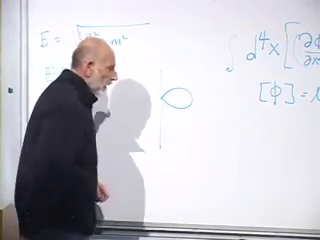
\includegraphics[width=0.72\textwidth]{lecture_03_figure_02.png}
\lectureframe{00:28:30.560}

\medskip
\begin{tikzpicture}[line width=0.8pt,scale=1.0]
  \draw[dashed] (-2.6,0) -- (0,0) -- (2.6,0);
  \fill (0,0) circle (0.055);
  \draw (0,0) .. controls (-0.85,0.7) and (-0.85,1.6) .. (0,1.6)
                .. controls (0.85,1.6) and (0.85,0.7) .. (0,0);
\end{tikzpicture}
\caption{Le tableau au moment du passage à l’auto-énergie scalaire, suivi d’un schéma prudent de la topologie du tadpole. La capture montre clairement la boucle, les formules de l’énergie relativiste et de l’énergie sans masse, ainsi qu’une partie de l’action ; elle ne permet pas d’affirmer que les coefficients et les légendes masqués sont visibles.}
\end{figure}

Au sommet, le scalaire peut être absorbé puis réémis, tandis que les deux autres branches se propagent du point à lui-même. À des facteurs numériques et combinatoires près, la correction vaut
\begin{equation}
\delta m_\phi^2\sim \lambda G_\phi(0).
\end{equation}
Dans l’approximation du continuum, le propagateur au point de coïncidence est infini. Une théorie effective ne prétend pas être valable à une distance arbitrairement courte ; imposons donc \(|\Delta|\geq\delta\). On obtient alors
\begin{equation}
G_\phi(0)\longrightarrow G_\phi(\delta)sim\frac{1}{\delta^2},
\qquad
\delta m_\phi^2\sim\frac{\lambda}{\delta^2}sim\lambda\Lambda^2.
\end{equation}
On parle de divergence quadratique car elle comporte deux puissances du cutoff en impulsion. L’intégration dans l’espace des impulsions conduit à la même conclusion : la contribution excessive provient des impulsions de boucle arbitrairement grandes. Que l’échelle minimale soit finalement fixée par la grande unification, la gravité quantique ou quelque chose qui reste à imaginer ne change rien au diagnostic de la théorie effective.

C’est un problème de réglage fin. Si \(\delta\) est extrêmement petit et si \(\lambda\) n’est pas extraordinairement minuscule, la correction radiative est bien supérieure à la masse au carré du scalaire observée à basse énergie. Le coefficient nu et la correction de boucle doivent alors s’annuler avec un nombre invraisemblable de chiffres de précision :
\begin{equation}
m_{\mathrm{physical}}^2
=m_{\mathrm{bare}}^2+\delta m_\phi^2.
\end{equation}
Le propagateur massif ne résout pas le problème. Aux distances responsables de la divergence, \(e^{-m|\Delta|}\simeq1\). La boucle ultraviolette a oublié la masse bien avant d’atteindre le cutoff.

\section{Dimensions du fermion et son propagateur}

Reprenons maintenant la même analyse dimensionnelle pour un fermion de Dirac. Son action libre est
\begin{equation}
S_\psi=\int d^4x\,
\bar\psi\left(i\gamma^\mu\partial_\mu-m\right)\psi.
\end{equation}
Les matrices gamma sont numériques et sans dimension. Comme le terme cinétique ne contient qu’une seule dérivée,
\begin{align}
1
&=L^4[\bar\psi]L^{-1}[\psi],\\
[\psi]=[\bar\psi]&=L^{-3/2}.
\end{align}
Les puissances demi-entières n’ont rien d’inquiétant ; les fermions font apparaître des moitiés en de nombreux endroits.

\begin{classroomqa}
\audiencequestion{Ne serait-il pas plus simple de déduire \([\psi]\) du terme de masse ? \lecturetimestamp{00:36:02}}
\lecturerresponse{Oui. Le terme de masse donne \(L^4L^{-1}[\bar\psi\psi]=1\), d’où \([\bar\psi\psi]=L^{-3}\) et \([\psi]=L^{-3/2}\). Nous avons commencé par la dérivation cinétique parce qu’elle reste pertinente dans la théorie sans masse et montre pourquoi la masse du fermion apparaît comme \(m\), et non comme \(m^2\).}
\end{classroomqa}

Deux champs fermioniques sont de dimension \(L^{-3}\) ; le raccourci dimensionnel employé dans le cours pour le propagateur sans masse est donc
\begin{equation}
S(\Delta)\sim\frac{1}{|\Delta|^3}.
\end{equation}
Rétablir sa structure matricielle donne au numérateur la forme plus précise exigée par la covariance de Lorentz :
\begin{equation}
S_{ij}(\Delta)
\propto
\frac{\left(\gamma_\mu\Delta^\mu\right)_{ij}}
{\left(\Delta^2\right)^2}.
\end{equation}
Le numérateur apporte une puissance de longueur et le dénominateur contient donc quatre puissances de l’intervalle ; la dimension nette reste \(L^{-3}\). Comme pour le scalaire, une masse fermionique supprime le propagateur à grande distance, mais ne modifie pas cette loi d’échelle à courte distance.

\section{Pourquoi une boucle fermionique fermée est négative}

Nous pouvons maintenant nous demander si un diagramme fermionique pourrait annuler la mauvaise auto-énergie bosonique. Le tadpole scalaire a un signe positif, à des facteurs numériques positifs près, tels que des puissances de \(\pi\) et des coefficients combinatoires. Une boucle fermionique fermée porte le signe opposé.

\begin{classroomqa}
\audiencequestion{Le signe moins de la boucle fermionique est-il lié à la discussion précédente sur une rotation complète ? \lecturetimestamp{00:40:21}}
\lecturerresponse{Il relève de la même structure de signes fermioniques, mais la démonstration utile ici repose sur l’antisymétrie par échange, plutôt que sur l’orientation géométrique d’une boucle. Coupons deux boucles, échangeons les particules identiques, puis reconnectons-les. L’échange transforme deux boucles en une seule et introduit un signe moins pour les fermions uniquement.}
\end{classroomqa}

Il vaut la peine de donner le raisonnement en détail. Supposons qu’un diagramme à une boucle ait le signe \(\sigma\), positif ou négatif. Deux boucles identiques et déconnectées ont le signe
\begin{equation}
\sigma^2=+1.
\end{equation}
Coupons simultanément les deux boucles. Deux particules identiques se propagent alors entre les points de coupure. Leur fonction d’onde ordinaire à deux particules est symétrique pour des bosons et antisymétrique pour des fermions :
\begin{align}
\Psi_B(x_1,x_2)&=+\Psi_B(x_2,x_1),\\
\Psi_F(x_1,x_2)&=-\Psi_F(x_2,x_1).
\end{align}
L’antisymétrie explique aussi le principe de Pauli : si l’on place les deux fermions dans le même état, l’échange ne change rien physiquement, mais doit inverser la fonction d’onde, qui doit donc s’annuler.

Reconnectons les lignes coupées après avoir échangé les deux particules. Du point de vue topologique, les deux boucles n’en forment plus qu’une. L’amplitude à deux boucles avant l’échange était positive. L’échange la laisse positive pour les bosons et en inverse le signe pour les fermions. Par conséquent,
\begin{equation}
\begin{aligned}
\operatorname{sign}(\text{closed boson loop})&=+1,\\
\operatorname{sign}(\text{closed fermion loop})&=-1.
\end{aligned}
\end{equation}
La conclusion est générale : chaque boucle fermionique fermée indépendante apporte un facteur \(-1\).

\section{La boucle de Yukawa}

Revenons à la masse du scalaire. Un boson ne peut pas se transformer en un fermion unique, car cela changerait la parité du nombre fermionique. La correction fermionique la plus simple consiste à faire se scinder le scalaire en une paire fermion-antifermion, qui parcourt une boucle avant de se recombiner. L’interaction est un couplage de Yukawa,
\begin{equation}
\mathcal L_Y=-g\phi\bar\psi\psi.
\end{equation}
Dans le cas du Higgs, les fermions peuvent être des quarks ou des leptons. Il y a deux points d’interaction, donc deux facteurs de \(g\).

Le tadpole scalaire impliquait un seul point, dont on pouvait fixer la position globale puisque l’invariance par translation ne fournit que le volume de l’espace-temps. La boucle de Yukawa implique deux points. On peut fixer l’un d’eux, ou, de façon équivalente, leur position moyenne, mais il faut intégrer sur leur séparation relative \(\Delta\). Chaque propagateur fermionique apporte le facteur à courte distance \(1/|\Delta|^3\), donc
\begin{equation}
\delta m_{\phi,F}^2
\sim
-g^2\int_{|\Delta|\geq\delta}d^4\Delta\,
\frac{1}{|\Delta|^6}.
\end{equation}

Après avoir écrit les deux propagateurs, l’intégrale sur la séparation et les deux couplages, le cours demande à la salle un dernier facteur. La réponse est le signe moins. Les deux propagateurs se referment en une boucle fermionique ; toute l’intégrale à courte distance, positive par ailleurs, est donc multipliée par \(-1\).

L’analyse dimensionnelle suffit déjà à déterminer la divergence. \(d^4\Delta\) fournit quatre puissances de longueur, tandis que le dénominateur en comporte six ; la seule échelle de longueur qui reste est celle du cutoff :
\begin{equation}
\int_{|\Delta|\geq\delta}
\frac{d^4\Delta}{|\Delta|^6}
\sim\frac{1}{\delta^2}.
\end{equation}
En coordonnées radiales euclidiennes à quatre dimensions, on peut l’expliciter :
\begin{equation}
\int_{\delta}^{R}d^4\Delta\,\frac{1}{|\Delta|^6}
=2\pi^2\int_{\delta}^{R}dr\,\frac{r^3}{r^6}
=\pi^2\left(\frac{1}{\delta^2}-\frac{1}{R^2}\right).
\end{equation}
Les traces de spineurs et les normalisations des propagateurs modifient le coefficient, mais pas la dépendance quadratique au cutoff.\editorialnote{L’intégrale radiale est une forme explicite classique de l’estimation dimensionnelle donnée dans le cours. Elle est écrite en distance euclidienne, où la positivité et le décompte des puissances ultraviolettes sont transparents.}

\begin{classroomqa}
\audiencequestion{Le choix des bornes d’intégration ou leur inversion peut-il changer le signe ? \lecturetimestamp{00:51:06}}
\lecturerresponse{Non. Il ne s’agit pas d’une intégrale unidimensionnelle orientée dont les bornes produiraient le signe physique. C’est une intégrale sur quatre composantes, ou, plus simplement, sur une mesure radiale positive. Sa contribution ultraviolette est positive. Le signe négatif provient uniquement de la boucle fermionique fermée.}
\end{classroomqa}

\begin{classroomqa}
\audiencequestion{Quelle est la dimension du couplage de Yukawa \(g\) ? \lecturetimestamp{00:51:51}}
\lecturerresponse{Il est sans dimension en quatre dimensions. Puisque \([\phi]=L^{-1}\) et \([\bar\psi\psi]=L^{-3}\), le produit \(\phi\bar\psi\psi\) est de dimension \(L^{-4}\), exactement compensée par \(d^4x\).}
\end{classroomqa}

La principale correction fermionique est donc
\begin{equation}
\delta m_{\phi,F}^2
\sim -C_F\frac{g^2}{\delta^2}
=-C_Fg^2\Lambda^2,
\end{equation}
où \(C_F>0\) regroupe des facteurs numériques, de spin et de multiplicité. La boucle scalaire prend la forme correspondante
\begin{equation}
\delta m_{\phi,B}^2
\sim+C_B\frac{\lambda}{\delta^2}
=+C_B\lambda\Lambda^2.
\end{equation}
Nous n’avons pas encore résolu le problème du réglage fin, mais nous avons trouvé un élément indispensable : une contribution de même degré ultraviolet et de signe opposé.

\section{Conditions nécessaires à l’annulation}

Ce serait une coïncidence extraordinaire que des couplages sans lien entre eux vérifient
\begin{equation}
C_B\lambda=C_Fg^2
\end{equation}
avec exactement la précision exigée par une grande hiérarchie d’échelles. Le cours résume cela par \(g^2=\lambda\), en omettant les facteurs dépendant des conventions et les facteurs de multiplicité. Une véritable solution exige une structure mathématique qui impose cette relation au lieu de simplement la permettre.

C’est ce qui motive la supersymétrie. Elle relie bosons et fermions et restreint leurs couplages à des combinaisons qui provoquent l’annulation de nombreux termes divergents autrement dangereux. L’annulation se reproduit alors dans plusieurs diagrammes parce qu’elle découle d’une symétrie, et non d’un ajustement des paramètres boucle après boucle.

L’égalité des masses importe également. Si les masses du boson et du fermion sont identiques, leurs propagateurs complets peuvent être appariés au mieux. Si elles diffèrent légèrement, les réponses complètes et finies ne s’annulent pas exactement, car les propagateurs diffèrent à des distances comparables à leurs longueurs de Compton. Leurs comportements asymptotiques communs à courte distance peuvent néanmoins annuler la partie divergente :
\begin{equation}
\mathcal I_B(\Delta)-\mathcal I_F(\Delta)
\quad\hbox{may be finite as}\quad \Delta\to0,
\end{equation}
où \(\mathcal I_B\) et \(\mathcal I_F\) désignent les intégrandes complets des boucles bosonique et fermionique, après prise en compte des sommets, des numérateurs et des multiplicités. On ne soustrait pas directement les propagateurs eux-mêmes, qui sont de dimensions différentes. Même lorsque les termes ultraviolets s’annulent, il peut subsister une contribution finie. C’est ce qui ouvre la voie à une supersymétrie approchée ou brisée. L’égalité exacte produit l’annulation la plus nette ; une brisure suffisamment contrôlée peut tout de même éliminer la catastrophe ultraviolette tout en laissant des écarts de masse observables.

Nous sommes ainsi parvenus à la supersymétrie sans encore en écrire l’algèbre. Le raisonnement est complet :
\begin{equation}
\begin{gathered}
G_\phi(\Delta)\sim \Delta^{-2},
\qquad
\delta m_{\phi,B}^2\sim+C_B\lambda\Lambda^2,\\[0.4em]
S_\psi(\Delta)\sim \Delta^{-3},
\qquad
\delta m_{\phi,F}^2\sim-C_Fg^2\Lambda^2,\\[0.4em]
\text{symmetry-enforced matching}\\
\Longrightarrow\quad
\text{quadratic divergences cancel}.
\end{gathered}
\end{equation}
Il reste à comprendre le principe abstrait de symétrie qui impose ces relations et à examiner des exemples concrets de son action.

\chapter{De la symétrie ordinaire à l’algèbre de Grassmann}

\lectureoverview{La supersymétrie est une symétrie. Commençons donc par rappeler ce que ce terme signifie en mécanique quantique. Une transformation physique est représentée dans l’espace de Hilbert par un opérateur unitaire ; les transformations continues sont engendrées infinitésimalement, et leurs commutateurs décrivent la composition des transformations. Une véritable symétrie conserve l’énergie, ce qui revient à commuter avec le hamiltonien. La supersymétrie modifie alors une hypothèse commune à tous les exemples familiers : ses générateurs transforment les bosons en fermions et les fermions en bosons. Leur construction conduit naturellement aux opérateurs de création et d’annihilation, aux anticommutateurs et à l’algèbre de Grassmann finie, dans laquelle les quantités impaires ont un carré nul.}

\section{La symétrie relie des configurations différentes}

Une symétrie n’est pas une simple régularité décorative. C’est une opération qui relie une configuration physique à une autre. La réflexion gauche-droite, par exemple, met en correspondance les deux mains. Si la personne et les lois qui l’entourent étaient exactement symétriques par réflexion gauche-droite, les propriétés correspondantes des deux mains seraient identiques. Plus généralement, des objets ou des états reliés par une symétrie exacte doivent partager les grandeurs physiques que cette symétrie conserve. En physique des particules, cela signifie souvent qu’ils ont la même masse ; en physique atomique, que les états d’un même multiplet de rotation ont la même énergie.

Notre objectif est la supersymétrie, mais commençons par rappeler les symétries continues, comme les rotations et les translations. Il est déjà délicat de savoir si la supersymétrie est « continue » au sens habituel. Ses paramètres infinitésimaux ne sont pas des nombres réels ordinaires commutatifs. Il vaut mieux la considérer comme une extension graduée des symétries continues ; l’arithmétique de Grassmann introduite ci-dessous rend cette formulation suffisamment précise pour nos besoins. \editorialnote{La terminologie moderne décrit la supersymétrie comme une symétrie continue graduée. Cette précision explique la mise en garde du cours : la distinction habituelle entre continu et discret ne s’applique pas aisément à la supersymétrie.}

\section{Opérations unitaires dans l’espace de Hilbert}

Un système quantique est représenté par un vecteur d’état \(\ket{\psi}\). Une opération de symétrie physique est représentée par un opérateur \(U\) agissant sur cet état :
\begin{equation}
\ket{\psi}\longmapsto U\ket{\psi}.
\end{equation}
Pour une rotation spatiale, l’axe et l’angle déterminent \(U\). Si un état contient des particules en plusieurs positions, le ket transformé les représente toutes à leurs positions après rotation. Une translation agit de façon analogue : l’état est remplacé par un état où toute la configuration est déplacée.

\begin{classroomqa}
\audiencequestion{Le vecteur d’état appartient à un espace de Hilbert souvent de dimension infinie. Fait-on tourner l’espace de Hilbert ou l’espace ordinaire à trois dimensions ? \lecturetimestamp{00:04:20}}
\lecturerresponse{Les deux descriptions renvoient à la même opération, considérée à des niveaux différents. La transformation unitaire agit sur le vecteur de l’espace de Hilbert et représente la rotation physique de la configuration dans l’espace ordinaire. Il ne s’agit pas d’une rotation littérale de l’espace de Hilbert abstrait en trois dimensions, mais de la représentation d’une rotation spatiale dans cet espace.}
\end{classroomqa}

La condition essentielle est l’unitarité :
\begin{equation}
U^\dagger U=UU^\dagger=\mathbf 1,
\qquad
U^{-1}=U^\dagger.
\end{equation}
Elle conserve les produits scalaires et donc les probabilités :
\begin{equation}
\braket{U\psi}{U\psi}
=\bra{\psi}U^\dagger U\ket{\psi}
=\braket{\psi}{\psi}.
\end{equation}

\begin{figure}[H]
\centering
\includegraphics[width=0.56\textwidth]{lecture_04_figure_02.png}
\lectureframe{00:05:56.420}
\caption{Transition précoce au tableau, de l’état transformé à la condition d’unitarité. Le ket et le produit avec l’adjoint sont visibles, mais l’enseignant en masque les extrémités droites ; les équations complètes figurent dans la démonstration ci-dessous.}
\end{figure}

À proprement parler, le théorème de Wigner autorise aussi des symétries antiunitaires, comme l’inversion du temps. Les transformations reliées continûment à l’identité, qui nous intéressent ici, sont représentées par des opérateurs unitaires. \editorialnote{Cette possibilité antiunitaire est une précision classique ; elle ne modifie pas l’analyse des rotations, des translations ni des générateurs de supersymétrie présentée dans le cours.}

\section{Transformations infinitésimales et générateurs}

L’opération qui ne fait rien est représentée par \(U=\mathbf 1\), et non par \(U=0\). Une transformation suffisamment petite diffère de l’identité par un terme linéaire en son petit paramètre. Pour une rotation d’un petit angle \(\epsilon\),
\begin{equation}
U(\epsilon)=\mathbf 1+i\epsilon L+O(\epsilon^2).
\end{equation}
L’unitarité au premier ordre impose
\begin{align}
U^\dagger U
&=\left(\mathbf 1-i\epsilon L^\dagger\right)
  \left(\mathbf 1+i\epsilon L\right)+O(\epsilon^2)\\
&=\mathbf 1+i\epsilon(L-L^\dagger)+O(\epsilon^2),
\end{align}
d’où
\begin{equation}
L^\dagger=L.
\end{equation}
L’opérateur \(L\) est le générateur infinitésimal.

Les rotations requièrent trois générateurs, un pour chaque axe indépendant :
\begin{equation}
L_x,\qquad L_y,\qquad L_z.
\end{equation}
Une rotation autour d’un axe arbitraire \(\widehat{\bm n}\) est engendrée par
\begin{equation}
L_{\widehat{\bm n}}=\widehat{\bm n}\cdot\bm L.
\end{equation}

\begin{classroomqa}
\audiencequestion{Peut-on additionner les générateurs associés aux axes \(x\), \(y\) et \(z\) pour obtenir une rotation autour d’un autre axe ? \lecturetimestamp{00:07:50}}
\lecturerresponse{Oui. Leurs combinaisons linéaires engendrent des rotations autour d’axes intermédiaires. Trois composantes indépendantes suffisent pour construire toute rotation spatiale infinitésimale.}
\end{classroomqa}

Pour les rotations, ces générateurs sont les composantes du moment cinétique. Cette notation est utile plus généralement, car toute symétrie continue s’appréhende localement à l’aide de ses générateurs.

\section{Le commutateur comme table de multiplication}

Les générateurs des rotations vérifient
\begin{align}
[L_x,L_y]&=iL_z,&
[L_y,L_z]&=iL_x,&
[L_z,L_x]&=iL_y,
\end{align}ou, sous une forme compacte,
\begin{equation}
[L_i,L_j]=i\epsilon_{ijk}L_k.
\end{equation}
Le symbole de Levi-Civita s’annule si deux indices sont égaux et vaut \(+1\) ou \(-1\) pour les permutations paires ou impaires de \(1,2,3\). Le fait structurel essentiel est la fermeture : le commutateur de deux générateurs est un autre générateur.

Pourquoi un commutateur décrit-il la géométrie des rotations ? Effectuons une petite rotation autour de \(x\), puis une autour de \(y\), annulons la rotation autour de \(x\), et enfin annulons celle autour de \(y\). Les opérations ne s’annulent pas, car les rotations autour d’axes différents ne commutent pas.

\begin{classroomqa}
\audiencequestion{Peut-on représenter cette non-commutativité avec les mouvements de roulis, de tangage et de lacet d’un avion ? \lecturetimestamp{00:12:36}}
\lecturerresponse{Oui. Des rotations successives autour des axes de l’avion illustrent immédiatement que changer leur ordre modifie son orientation finale. L’algèbre ci-dessous est la version infinitésimale de ce fait bien connu.}
\end{classroomqa}

Posons
\begin{equation}
U_x(\epsilon)=\mathbf 1+i\epsilon L_x,
\qquad
U_y(\delta)=\mathbf 1+i\delta L_y.
\end{equation}
Comme les opérateurs agissent sur les kets de droite à gauche, la séquence indiquée est représentée par
\begin{equation}
\mathcal C
=U_y^{-1}(\delta)U_x^{-1}(\epsilon)
 U_y(\delta)U_x(\epsilon).
\end{equation}

\begin{classroomqa}
\audiencequestion{Pourquoi peut-on écrire les opérations qui annulent les rotations comme des inverses plutôt que comme des adjoints ? \lecturetimestamp{00:13:25}}
\lecturerresponse{Parce que les transformations sont unitaires : \(U^\dagger=U^{-1}\). Pour une transformation infinitésimale, prendre l’inverse revient simplement à changer le signe du terme du premier ordre, \(U_x^{-1}=\mathbf 1-i\epsilon L_x+O(\epsilon^2)\).}
\end{classroomqa}

La multiplication au tableau des quatre facteurs a donné lieu à un exercice animé : tous les termes linéaires en \(\epsilon\) ou \(\delta\) s’annulent, la salle a suivi les termes mixtes, et une confusion passagère sur un facteur deux a montré combien il est facile de perdre l’ordre des opérateurs. Le résultat propre au deuxième ordre est
\begin{align}
\mathcal C
&=\mathbf 1+\epsilon\delta[L_x,L_y]
  +O(\epsilon^2\delta,\epsilon\delta^2)\\
&=\mathbf 1+i\epsilon\delta L_z
  +O(\epsilon^2\delta,\epsilon\delta^2).
\end{align}
La séquence fermée laisse donc une petite rotation autour de \(z\), d’un angle proportionnel à \(\epsilon\delta\). \editorialnote{La multiplication affichée fixe l’ordre et le coefficient après le calcul exploratoire fait en classe. Inverser la convention de la séquence change le signe, mais ne modifie pas la conclusion : la transformation résiduelle est gouvernée par le commutateur.}

\begin{classroomqa}
\audiencequestion{Si l’on changeait l’ordre des opérations inverses, le produit serait-il égal à l’identité ? \lecturetimestamp{00:25:23}}
\lecturerresponse{Si chaque transformation était placée juste à côté de son inverse, les paires s’annuleraient. La séquence de commutateur non triviale sépare délibérément ces paires ; le fait qu’elle ne se réduise pas à l’identité mesure la dépendance à l’ordre.}
\end{classroomqa}

Les produits plus longs deviennent certes plus compliqués, mais n’introduisent aucun principe nouveau.

\begin{classroomqa}
\audiencequestion{Que se passe-t-il avec plus de trois générateurs ou avec de nombreuses petites transformations ? \lecturetimestamp{00:25:34}}
\lecturerresponse{Il y a davantage de commutateurs et de calculs à suivre, mais connaître l’algèbre fermée permet de déterminer comment se combinent un nombre arbitraire de transformations infinitésimales. On peut construire les transformations finies à partir d’un grand nombre de petites transformations.}
\end{classroomqa}

En ce sens, l’algèbre des commutateurs est la table de multiplication d’un groupe continu, écrite au voisinage de l’identité.

\section{Les translations complètent l’exemple spatial}

Les translations spatiales sont engendrées par la quantité de mouvement. Avec la convention de signe utilisée dans le cours,
\begin{equation}
\begin{aligned}
T_x(a)&=\mathbf 1+iaP_x+O(a^2),\\
T_y(b)&=\mathbf 1+ibP_y+O(b^2),
\end{aligned}
\end{equation}
où \(a\) et \(b\) désignent des distances, et non des angles.

Deux translations commutent. Déplaçons un point selon \(x\), puis selon \(y\), annulons la translation selon \(x\), puis celle selon \(y\) ; le point revient à son origine :
\begin{equation}
[P_i,P_j]=0.
\end{equation}

\begin{classroomqa}
\audiencequestion{Faut-il exercer des forces sur un objet physique pour le mettre en mouvement et l’arrêter lors d’une translation ou d’une rotation ? \lecturetimestamp{00:28:45}}
\lecturerresponse{Ce n’est pas l’opération définie ici. Une transformation de symétrie compare l’état initial à l’état mathématique dans lequel toute la configuration a été déplacée ou tournée. Elle ne décrit ni une trajectoire dynamique, ni une accélération, ni le travail effectué pendant le déplacement de l’appareil.}
\end{classroomqa}

Une rotation et une translation ne commutent pas. Translatons un point, faisons-le tourner autour de l’origine, effectuons une translation inverse le long de l’axe initial, puis annulons la rotation ; le point ne revient pas à sa position de départ. L’algèbre mixte est
\begin{equation}
[L_i,P_j]=i\epsilon_{ijk}P_k.
\end{equation}
Cette relation signifie que la quantité de mouvement elle-même se transforme comme un vecteur sous l’effet des rotations. Le calcul précis sur les indices importe moins ici que la leçon générale : les transformations de l’espace euclidien sont encodées dans les commutateurs entre les générateurs de rotation et de translation.

\section{Une symétrie doit conserver l’énergie}

Passons maintenant de la composition des transformations à la dynamique. Si \(U\) est une véritable symétrie du système, son application ne peut pas modifier l’énergie. Soit \(\ket{E}\) un état propre de l’énergie :
\begin{equation}
H\ket{E}=E\ket{E}.
\end{equation}
Le symbole \(E\) à droite est un nombre ; \(\ket{E}\) est un vecteur propre associé à cette valeur propre.

\begin{figure}[H]
\centering
\begin{minipage}[t]{0.43\textwidth}
\centering
\includegraphics[width=\linewidth]{lecture_04_figure_03.png}
\lectureframe{00:34:38.239}
\end{minipage}
\hfill
\begin{minipage}[t]{0.50\textwidth}
\centering
\includegraphics[width=\linewidth]{lecture_04_figure_04.png}
\lectureframe{00:36:22.376}
\end{minipage}
\caption{Le ket transformé \(U\ket{E}\) et l’équation propre qui le définit \(H\ket{E}=E\ket{E}\), isolés dans deux images successives au tableau.}
\end{figure}

Si \(U\) est une symétrie, alors \(U\ket{E}\) possède la même valeur propre :
\begin{equation}
HU\ket{E}=EU\ket{E}.
\end{equation}
Comme \(E\) est un scalaire, il commute avec \(U\), et on peut utiliser l’équation propre initiale :
\begin{align}
HU\ket{E}
&=EU\ket{E}\\
&=UE\ket{E}\\
&=UH\ket{E}.
\end{align}
Par conséquent,
\begin{equation}
(HU-UH)\ket{E}=0.
\end{equation}

\begin{classroomqa}
\audiencequestion{Peut-on reprendre la démonstration à partir de sa première relation ? \lecturetimestamp{00:35:55}}
\lecturerresponse{Partons de \(H\ket{E}=E\ket{E}\). Par symétrie, \(U\ket{E}\) a la même énergie, donc \(HU\ket{E}=EU\ket{E}\). Faisons passer le scalaire \(E\) à travers \(U\), remplaçons \(E\ket{E}\) par \(H\ket{E}\), puis soustrayons. On obtient \((HU-UH)\ket{E}=0\).}
\end{classroomqa}

\begin{figure}[H]
\centering
\includegraphics[width=0.70\textwidth]{lecture_04_figure_05.png}
\lectureframe{00:38:51.066}
\caption{La démonstration complète au tableau. Des traits courbes relient l’égalité des énergies à la substitution \(E\ket{E}=H\ket{E}\) ; la dernière ligne est \((HU-UH)\ket{E}=0\).}
\end{figure}

Le raisonnement vaut pour chaque état propre de l’énergie. En supposant que ces états forment une base complète, tout opérateur qui annule chacun d’eux est l’opérateur nul :
\begin{equation}
[H,U]=0.
\end{equation}
C’est le critère pour qu’une transformation unitaire indépendante du temps soit une symétrie du hamiltonien.

Pour une transformation infinitésimale,
\begin{equation}
U(\epsilon)=\mathbf 1+i\epsilon L_i+O(\epsilon^2),
\end{equation}
l’identité commute déjà avec \(H\) ; chaque générateur doit donc vérifier
\begin{equation}
[L_i,H]=0.
\end{equation}

\begin{figure}[H]
\centering
\includegraphics[width=0.47\textwidth]{lecture_04_figure_06.png}
\lectureframe{00:42:14.296}
\caption{Le critère de symétrie résumé au tableau : \([U,H]=0\), puis sa forme exprimée en termes de générateurs, normalisée à partir de l’inscription peu lisible au bas du tableau : \([L_i,H]=0\).}
\end{figure}

Si \(L_i\) ne dépend pas explicitement du temps, l’équation de Heisenberg donne
\begin{equation}
\frac{dL_i}{dt}
=i[H,L_i]=0
\qquad(\hbar=1).
\end{equation}
Les générateurs de symétrie sont donc des charges conservées. La symétrie par translation spatiale entraîne la conservation de la quantité de mouvement ; la symétrie de rotation, celle du moment cinétique. \editorialnote{La précision concernant la dérivée explicite par rapport au temps est standard et reste implicite dans l’énoncé de conservation du cours.}

\section{Transformer le système physique tout entier}

L’expression « la rotation est une symétrie » peut être employée à tort si l’on ne transforme qu’une partie de l’appareil. On peut faire tourner un spin libre sans modifier son énergie. En revanche, si on le place dans un champ magnétique fixe et qu’on ne fait tourner que le spin, son énergie de Zeeman change. Cela ne réfute pas la symétrie de rotation : le champ était maintenu fixe tandis que le spin tournait par rapport à lui. Si l’on fait tourner ensemble le spin et le champ, ou si l’on utilise un champ extérieur lui-même invariant, l’énergie reste inchangée.

La même difficulté se présente pour l’atome d’hydrogène. Translater l’électron seul par rapport au proton modifie leur séparation et, par conséquent, l’énergie coulombienne. La symétrie de translation agit sur tout le système électron-proton et déplace les deux d’une même distance.

\begin{classroomqa}
\audiencequestion{Le champ extérieur doit-il lui-même posséder cette symétrie ? \lecturetimestamp{00:43:09}}
\lecturerresponse{Il faut soit que le champ extérieur fixe soit déjà invariant sous l’opération, soit qu’il soit transformé en même temps que le reste du système. Une rotation relative du spin par rapport à un champ qui ne tourne pas correspond à une configuration physique différente, et non à la transformation de symétrie de l’ensemble du dispositif.}
\end{classroomqa}

La dégénérescence due aux rotations dans un atome en donne un exemple positif clair. Pour un moment cinétique fixé \(l\), les rotations mélangent les états de nombres quantiques magnétiques
\begin{equation}
m=-l,-l+1,\ldots,l.
\end{equation}
En l’absence de champ magnétique ou électrique extérieur, tous les états du multiplet ont la même énergie :
\begin{equation}
E_{l,m}=E_l.
\end{equation}
La symétrie relie des états distincts et impose leur dégénérescence.

\section{Ce que change la supersymétrie}

Toutes les symétries familières abordées jusqu’ici préservent la nature bosonique ou fermionique. Une rotation transforme un électron en un autre électron, pas en photon. Les rotations de couleur mélangent les trois couleurs d’un quark, mais ne transforment pas celui-ci en gluon. Les symétries internes et spatio-temporelles ordinaires peuvent mélanger des composantes ou des nombres quantiques, mais leurs générateurs sont bosoniques et ne modifient pas la parité fermionique.

La supersymétrie est différente :
\begin{equation}
Q\ket{B}\sim\ket{F},
\qquad
Q\ket{F}\sim\ket{B}.
\end{equation}
Ses multiplets franchissent la frontière entre bosons et fermions. Dans une théorie exactement supersymétrique, les partenaires d’un même multiplet ont la même masse. C’est précisément l’appariement requis dans les cours précédents : les boucles bosoniques et fermioniques appariées peuvent annuler les grandes corrections ultraviolettes aux masses des scalaires. Cette construction est difficile à visualiser, car aucun mouvement spatial ordinaire ne transforme un état de spin entier en un état de spin demi-entier. Nous allons donc procéder par l’algèbre.

\section{Un supercharge prototype}

Soit \(A,A^\dagger\) l’opérateur qui annihile et crée un boson, et \(C,C^\dagger\) celui qui annihile et crée un fermion. L’opérateur hermitien le plus simple qui échange leurs états à une particule est
\begin{equation}
Q=C^\dagger A+A^\dagger C.
\end{equation}
Le premier terme annihile un boson et crée un fermion ; le second annihile un fermion et crée un boson. Si \(Q\) agit sur un état à un boson, le terme \(A^\dagger C\) s’annule, car aucun fermion n’est présent pour être annihilé, tandis que \(C^\dagger A\) opère la conversion. Les rôles sont inversés pour un état à un fermion.

\begin{classroomqa}
\audiencequestion{Cette construction crée-t-elle une particule unique qui serait une superposition d’un boson et d’un fermion ? \lecturetimestamp{00:52:37}}
\lecturerresponse{\(Q\) est un opérateur, et non un état. Agissant sur un état purement bosonique, il produit un état fermionique ; agissant sur un état purement fermionique, il produit un état bosonique. S’il agit linéairement sur une superposition déjà générale, il produit une autre superposition, comme le ferait tout opérateur linéaire.}
\end{classroomqa}

La salle met ensuite le vide à l’épreuve. Puisque les deux opérateurs d’annihilation l’annulent,
\begin{equation}
A\ket{0}=0,\qquad C\ket{0}=0,
\end{equation}
on a
\begin{equation}
Q\ket{0}=0.
\end{equation}
Le résultat est le vecteur nul, et non une deuxième copie du vide.

Le modèle est volontairement schématique. Un boson de spin zéro peut être transformé en l’une ou l’autre des composantes d’un fermion de spin un demi ; le générateur doit donc porter un indice de spineur :
\begin{equation}
Q_\alpha\ket{B}\sim\ket{F_\alpha}.
\end{equation}
Dans la représentation simplifiée à deux composantes du cours,
\begin{equation}
Q_\alpha\ket{F_\beta}\sim\delta_{\alpha\beta}\ket{B}.
\end{equation}

\begin{classroomqa}
\audiencequestion{Comment les dimensions des espaces d’états peuvent-elles correspondre alors qu’un boson de spin zéro a une composante de spin et un fermion de spin un demi en a deux ? \lecturetimestamp{00:55:02}}
\lecturerresponse{Un \(Q\) sans indice ne suffit pas. Il existe des composantes de spineur \(Q_\alpha\), chacune pouvant produire l’une des composantes de spin du fermion. Le supercharge lui-même porte un demi-spin, puisqu’il modifie le spin d’une demi-unité.}
\end{classroomqa}

Les \(Q_\alpha\) sont des opérateurs fermioniques ou, plus précisément, impairs au sens de Grassmann. Chacun de leurs termes contient un nombre impair d’opérateurs fermioniques, d’où l’inversion de la parité fermionique. Les observables mesurables ordinaires sont paires. Il faut distinguer un supercharge impair de son paramètre de transformation impair : une transformation supersymétrique finie est construite à partir d’une combinaison paire telle que \(\epsilon^\alpha Q_\alpha+\bar\epsilon_{\dot\alpha}\bar Q^{\dot\alpha}\), où \(\epsilon\) et \(Q\) sont tous deux impairs. \editorialnote{Dans le cours, les générateurs sont appelés de manière informelle nombres de Grassmann. Plus précisément, les supercharges sont des opérateurs impairs, tandis que les paramètres anticommutatifs sont des nombres de Grassmann ; leur produit est pair et peut intervenir dans une transformation finie.}

\section{Algèbres des opérateurs bosoniques et fermioniques}

Pour des modes bosoniques étiquetés par \(i,j\),
\begin{align}
[A_i,A_j]&=0,&
[A_i^\dagger,A_j^\dagger]&=0,&
[A_i,A_j^\dagger]&=\delta_{ij}.
\end{align}
Les étiquettes peuvent désigner l’impulsion, la position, le spin ou n’importe quelle base complète à une particule. Les opérateurs de création commutant,
\begin{equation}
A_i^\dagger A_j^\dagger\ket{0}
=A_j^\dagger A_i^\dagger\ket{0}.
\end{equation}
l’état à deux bosons est symétrique par échange.

Les opérateurs fermioniques vérifient des relations d’anticommutation :
\begin{align}
\{C_i,C_j\}&=0,&
\{C_i^\dagger,C_j^\dagger\}&=0,&
\{C_i,C_j^\dagger\}&=\delta_{ij},
\end{align}
où
\begin{equation}
\{X,Y\}=XY+YX.
\end{equation}
Pour un mode unique,
\begin{equation}
\{C^\dagger,C^\dagger\}=2(C^\dagger)^2=0,
\end{equation}
donc
\begin{equation}
(C^\dagger)^2=0.
\end{equation}
L’opérateur n’est pas nul ; c’est son carré qui est nul. Il peut créer un fermion dans le mode, mais une seconde application donne zéro. C’est le principe d’exclusion de Pauli exprimé dans le langage des opérateurs.

Pour des étiquettes distinctes,
\begin{equation}
C_i^\dagger C_j^\dagger\ket{0}
=-C_j^\dagger C_i^\dagger\ket{0},
\end{equation}
ce qui exprime l’antisymétrie de l’état à deux fermions. Le remplacement algébrique
\begin{equation}
\begin{gathered}
\text{bosons: commutators}\\
\Updownarrow\\
\text{fermions: anticommutators}
\end{gathered}
\end{equation}
encode la distinction statistique.

Un même mode peut accueillir de nombreux bosons. Un grand nombre de photons peut donc se comporter comme un champ électromagnétique classique, doté d’une amplitude numérique ordinaire. Les fermions, eux, ne peuvent pas s’accumuler dans un même mode, et un champ fermionique impair ne prend pas de valeur classique ordinaire commutative. D’où l’intérêt d’une autre arithmétique pour gérer les signes fermioniques.

\section{Nombres de Grassmann et parité}

Les nombres ordinaires commutent :
\begin{equation}
\alpha_i\alpha_j=\alpha_j\alpha_i.
\end{equation}
Les générateurs de Grassmann anticommutent :
\begin{equation}
\theta_i\theta_j=-\theta_j\theta_i.
\end{equation}
Posons \(i=j\), dans un système numérique où \(2\neq0\) ; on obtient alors
\begin{equation}
\theta_i^2=0.
\end{equation}
On ne peut attribuer à \(\theta_i\) aucune valeur numérique ordinaire, telle que six ou sept. Ces symboles forment une algèbre conçue pour suivre les signes fermioniques.

Les coefficients ordinaires commutent avec les générateurs de Grassmann :
\begin{equation}
\alpha\theta_i=\theta_i\alpha.
\end{equation}

\begin{classroomqa}
\audiencequestion{Quel type d’objet obtient-on en multipliant un nombre ordinaire par un nombre de Grassmann ? \lecturetimestamp{01:12:32}}
\lecturerresponse{Il reste impair au sens de Grassmann. La multiplication par un coefficient ordinaire en modifie l’échelle, mais pas la parité. L’espace vectoriel engendré par les générateurs est défini sur les nombres ordinaires.}
\end{classroomqa}

L’algèbre possède une parité \(\mathbb Z_2\). Les coefficients ordinaires et les produits d’un nombre pair de générateurs sont pairs ; un générateur ou un produit d’un nombre impair de générateurs est impair :
\begin{equation}
\begin{aligned}
\text{even}\cdot\text{even}&=\text{even},\\
\text{even}\cdot\text{odd}&=\text{odd},\\
\text{odd}\cdot\text{odd}&=\text{even}.
\end{aligned}
\end{equation}

\begin{classroomqa}
\audiencequestion{Est-ce comparable aux règles de multiplication des nombres réels et imaginaires, ou s’agit-il d’une généralisation, comme l’introduction de \(i\) ? \lecturetimestamp{01:14:25}}
\lecturerresponse{C’est une généralisation de l’arithmétique, mais il ne faut pas pousser trop loin l’analogie. Les nombres imaginaires commutent toujours et vérifient \(i^2=-1\) ; les quantités impaires de Grassmann anticommutent et ont un carré nul. Le fait que les deux algèbres partagent la même règle de multiplication pair-impair ne les rend pas identiques.}
\end{classroomqa}

Un produit tel que \(\theta_1\theta_2\) est pair et commute avec tout élément homogène de l’algèbre de Grassmann, mais ce n’est pas un nombre ordinaire. Il est non nul, alors que
\begin{equation}
(\theta_1\theta_2)^2=0.
\end{equation}

\begin{classroomqa}
\audiencequestion{Si \(\theta_1\theta_2\) est pair, pourquoi n’est-ce pas simplement un nombre ordinaire ? \lecturetimestamp{01:17:36}}
\lecturerresponse{La parité paire signifie que l’élément commute dans l’algèbre graduée ; elle ne signifie pas qu’il s’agit d’un scalaire réel ou complexe. Sa nilpotence le distingue immédiatement d’un nombre ordinaire non nul.}
\end{classroomqa}

\section{Fonctions des variables de Grassmann}

Avec un seul générateur, tout polynôme s’arrête au premier ordre :
\begin{equation}
f(\theta)=\alpha+\beta\theta.
\end{equation}
Toutes les puissances \(\theta^n\) avec \(n\geq2\) sont nulles. Avec deux générateurs, l’élément le plus général est
\begin{equation}
f(\theta_1,\theta_2)
=\alpha+\beta_1\theta_1+\beta_2\theta_2
+\gamma\theta_1\theta_2.
\end{equation}
Écrire le dernier monôme dans l’ordre inverse en change le signe :
\begin{equation}
\theta_2\theta_1=-\theta_1\theta_2.
\end{equation}

\begin{classroomqa}
\audiencequestion{Multiplier \(\theta_1\) par un coefficient \(\beta\) crée-t-il une troisième variable de Grassmann indépendante ? \lecturetimestamp{01:18:39}}
\lecturerresponse{Non. Cela donne un autre vecteur de l’espace engendré par \(\theta_1\), et non un nouveau générateur de base. Avec deux générateurs indépendants, tout terme linéaire impair s’écrit \(\beta_1\theta_1+\beta_2\theta_2\).}
\end{classroomqa}

Pour trois générateurs, la base ordonnée est
\begin{equation}
1,\quad
\theta_1,\theta_2,\theta_3,\quad
\theta_1\theta_2,\theta_1\theta_3,\theta_2\theta_3,\quad
\theta_1\theta_2\theta_3.
\end{equation}
En général, \(n\) générateurs produisent \(2^n\) monômes de base ordonnés. Toute fonction analytique d’un nombre fini de générateurs de Grassmann se tronque à un tel polynôme, car les générateurs répétés s’annulent. \editorialnote{La base de dimension \(2^n\) explicite le motif que le cours construit pour un, deux et trois générateurs.}

\section{Dérivation de Grassmann}

Pour une variable, définissons
\begin{equation}
\frac{\partial}{\partial\theta}\alpha=0,
\qquad
\frac{\partial}{\partial\theta}\theta=1,
\end{equation}
de sorte que
\begin{equation}
\frac{\partial}{\partial\theta}
(\alpha+\beta\theta)=\beta.
\end{equation}
Pour deux variables, choisissons les dérivées à gauche et conservons l’ordre canonique \(\theta_1\theta_2\) :
\begin{align}
\frac{\partial^L f}{\partial\theta_1}
&=\beta_1+\gamma\theta_2,\\
\frac{\partial^L f}{\partial\theta_2}
&=\beta_2-\gamma\theta_1.
\end{align}
Le signe moins dans la deuxième ligne vient du fait que la dérivée impaire doit passer devant \(\theta_1\) avant de dériver \(\theta_2\).

C’est la règle du produit graduée. Si \(A\) est de parité \(|A|\in\{0,1\}\), alors
\begin{equation}
\frac{\partial^L}{\partial\theta}(AB)
=\left(\frac{\partial^L A}{\partial\theta}\right)B
+(-1)^{|A|}A
\left(\frac{\partial^L B}{\partial\theta}\right).
\end{equation}
L’esprit de la règle est ordinaire, mais elle comporte le signe qu’impose l’anticommutation. On peut aussi définir l’intégration de Grassmann ; comme l’espace des fonctions est fini, elle se réduit à un petit tableau. Le cours remet ce tableau à plus tard.

\section{Le mystère de l’exponentielle résolu}

Avec un seul générateur de Grassmann et un coefficient ordinaire \(a\),
\begin{equation}
e^{a\theta}
=1+a\theta,
\end{equation}
car toutes les puissances supérieures s’annulent. Deux exponentielles faisant intervenir le même générateur vérifient
\begin{align}
e^{a\theta}e^{b\theta}
&=(1+a\theta)(1+b\theta)\\
&=1+(a+b)\theta\\
&=e^{(a+b)\theta}.
\end{align}

La salle examine ensuite des générateurs distincts. Le calcul direct donne
\begin{equation}
e^{\theta_1}e^{\theta_2}
=(1+\theta_1)(1+\theta_2)
=1+\theta_1+\theta_2+\theta_1\theta_2.
\end{equation}
Au premier abord, le développement au tableau laisse penser que le carré de \(\theta_1+\theta_2\) pourrait fournir le dernier terme. Une personne dans l’assistance repère le signe :
\begin{equation}
(\theta_1+\theta_2)^2
=\theta_1^2+\theta_1\theta_2
 +\theta_2\theta_1+\theta_2^2
=0.
\end{equation}

\begin{classroomqa}
\audiencequestion{Le terme au carré s’annule-t-il parce qu’il contient \(\theta_1\theta_2+\theta_2\theta_1\) ? \lecturetimestamp{01:24:00}}
\lecturerresponse{Oui. Cette correction change la conclusion : \(e^{\theta_1+\theta_2}=1+\theta_1+\theta_2\), alors que le produit ordonné \(e^{\theta_1}e^{\theta_2}\) contient aussi \(\theta_1\theta_2\). La loi naïve d’addition des exposants ne s’applique pas à des exposants distincts qui anticommutent.}
\end{classroomqa}

Il n’y a pas de contradiction. Même pour des matrices ordinaires, \(e^Ae^B=e^{A+B}\) seulement si \(A\) et \(B\) commutent. Ici,
\begin{equation}
[\theta_1,\theta_2]
=\theta_1\theta_2-\theta_2\theta_1
=2\theta_1\theta_2.
\end{equation}
Ce commutateur est pair et commute avec les deux générateurs ; la série de Baker-Campbell-Hausdorff s’arrête donc :
\begin{equation}
e^{\theta_1}e^{\theta_2}
=\exp\left(
\theta_1+\theta_2+\frac12[\theta_1,\theta_2]
\right)
=e^{\theta_1+\theta_2+\theta_1\theta_2}.
\end{equation}
Comme l’exposant à droite est nilpotent, son développement donne exactement
\(1+\theta_1+\theta_2+\theta_1\theta_2\). \editorialnote{Ce calcul de Baker-Campbell-Hausdorff résout la question laissée ouverte à la fin du cours en direct. Le cours découvre correctement l’échec de la loi naïve, mais s’arrête avant d’identifier le terme de commutateur manquant.}

\begin{classroomqa}
\audiencequestion{De quel type de nombre s’agit-il, \(1+\theta_1\), et peut-on additionner des parties ordinaires et des parties de Grassmann ? \lecturetimestamp{01:26:16}}
\lecturerresponse{C’est un élément non homogène de l’algèbre de Grassmann, composé d’une partie paire \(1\) et d’une partie impaire \(\theta_1\). De telles sommes sont admises, mais ce ne sont ni des scalaires ordinaires ni des éléments impairs homogènes.}
\end{classroomqa}

Vers la fin, on examine un autre paradoxe apparent :
\begin{equation}
(\theta_1+\theta_2)^2=0.
\end{equation}
Cela n’implique pas que \(\theta_1\theta_2=0\), car les deux termes croisés s’annulent entre eux au lieu de s’annuler séparément.

\begin{classroomqa}
\audiencequestion{Si le carré de tout élément de Grassmann impair est nul, cela signifie-t-il que le produit de deux générateurs de Grassmann quelconques est nul ? \lecturetimestamp{01:32:19}}
\lecturerresponse{Non. L’équation \((\theta_1+\theta_2)^2=0\) signifie que \(\theta_1\theta_2+\theta_2\theta_1=0\). Elle établit l’anticommutation, et non la nullité de l’un ou l’autre des produits ordonnés. Le produit de générateurs distincts peut être non nul.}
\end{classroomqa}

\begin{classroomqa}
\audiencequestion{Lorsque nous écrivons ces exponentielles, supposons-nous la définition habituelle par série entière ? \lecturetimestamp{01:34:42}}
\lecturerresponse{Oui, et cette définition est cohérente, car chaque série s’arrête. Ce qui échoue, ce n’est pas l’exponentielle elle-même, mais l’identité non justifiée \(e^Ae^B=e^{A+B}\) pour \(A\) et \(B\) qui ne commutent pas. Le terme correctif faisant intervenir le commutateur rétablit la loi de composition appropriée.}
\end{classroomqa}

Cette conclusion exploratoire est appropriée. Les symétries ordinaires nous ont menés des transformations unitaires aux générateurs et aux commutateurs ; la supersymétrie nous a menés des générateurs impairs aux variables anticommutantes. Dans les deux cas, la loi de multiplication est l’objet central. Pour les rotations, elle apparaît dans \([L_i,L_j]\) ; pour les exponentielles de Grassmann, elle apparaît dans le terme de commutateur qui empêche l’addition naïve. L’algèbre est inhabituelle, mais cohérente, finie et précisément adaptée aux transformations fermioniques qu’exige la supersymétrie.

\chapter{Charges supersymétriques, fermeture et superspace}

\lectureoverview{La supersymétrie est difficile, non pas parce que ses règles sont nombreuses, mais parce qu’elles réunissent des idées que la physique ordinaire tient séparées. Nous commencerons par les variables de Grassmann, dont les éléments impairs anticommutent et dont les fonctions s’arrêtent après un nombre fini de termes. L’algèbre de leurs dérivées fournit ensuite le modèle des générateurs de symétrie impairs. Un oscillateur bosonique et un oscillateur fermionique donnent les charges supersymétriques les plus simples : leur anticommutateur est le Hamiltonien, si bien que l’échange des bosons et des fermions est indissociable d’une translation dans le temps. La même algèbre peut être représentée géométriquement par des translations dans les directions de Grassmann d’un espace-temps élargi appelé superspace.}

\section{Pourquoi revenir en arrière avant d’avancer}

La supersymétrie est l’une des constructions les plus abstraites de la physique. Comme les rotations et les translations, elle est une symétrie, mais elle ne s’inscrit pas dans l’espace-temps ordinaire sans élargir le sens que nous donnons au mot coordonnée. Ses paramètres naturels sont des quantités de Grassmann : des objets que l’on peut additionner et multiplier, mais qui anticommutent au lieu de commuter.

C’est pourquoi s’attaquer directement à l’algèbre finale ne serait pas utile. Nous commencerons par rendre l’arithmétique impaire maniable, puis nous rappellerons comment s’organisent les symétries continues ordinaires, avant de réunir ces deux idées. Le chemin est plus long, mais chaque étape prépare la suivante.

\section{L’algèbre de Grassmann en pratique}

\subsection{Éléments pairs et impairs}

Soit \(\epsilon_i\) des générateurs indépendants de Grassmann. Ils vérifient
\begin{equation}
\epsilon_i\epsilon_j=-\epsilon_j\epsilon_i,
\qquad
\{\epsilon_i,\epsilon_j\}=0.
\end{equation}
En posant \(i=j\), on obtient
\begin{equation}
2\epsilon_i^2=0,
\qquad
\epsilon_i^2=0,
\end{equation}
sur les nombres réels ou complexes. Le générateur n’est pas nul ; seul son carré est nul.

Chaque élément homogène a une parité. Un produit contenant un nombre impair de générateurs de Grassmann est impair, tandis qu’un produit qui en contient un nombre pair est pair :
\begin{align}
\text{odd}\times\text{odd}&=\text{even},\\
\text{odd}\times\text{even}&=\text{odd},\\
\text{even}\times\text{even}&=\text{even}.
\end{align}
Les éléments pairs commutent avec les éléments homogènes. Deux éléments impairs anticommutent. Ainsi,
\begin{equation}
n\epsilon_i=\epsilon_i n,
\qquad
\epsilon_i\epsilon_j=-\epsilon_j\epsilon_i,
\end{equation}
lorsque \(n\) est pair.

Un élément pair n’est pas nécessairement un nombre réel ou complexe ordinaire. Le produit
\(\epsilon_1\epsilon_2\), par exemple, est pair et nilpotent. Les nombres ordinaires constituent la partie scalaire de l’algèbre, tandis que les produits pairs fournissent d’autres éléments commutants.

\begin{classroomqa}
\audiencequestion{Y a-t-il une différence entre l’algèbre de Grassmann et les nombres de Grassmann, ou s’agit-il de la même chose ? \lecturetimestamp{00:06:45}}
\lecturerresponse{Les éléments sont les nombres de Grassmann ; l’algèbre est l’ensemble de ces éléments, muni de ses règles d’addition et de multiplication. On peut donc parler, de façon approximative, d’un même objet, mais il est utile de distinguer les objets que l’on manipule des règles qui régissent ces manipulations.}
\end{classroomqa}

\subsection{Les fonctions s’arrêtent}

Une fonction d’une variable de Grassmann ne comporte que deux puissances possibles :
\begin{equation}
f(\epsilon)=a+b\epsilon.
\end{equation}
Il n’y a pas de terme en \(\epsilon^2\). Avec deux générateurs indépendants,
\begin{equation}
f(\epsilon_1,\epsilon_2)
=a+b_1\epsilon_1+b_2\epsilon_2+c\epsilon_1\epsilon_2.
\end{equation}
le développement s’arrête dès que les deux générateurs sont apparus. Pour \(n\) générateurs indépendants, les monômes ordonnés forment une base de dimension \(2^n\) :
\begin{equation}
1,\quad
\epsilon_i,\quad
\epsilon_i\epsilon_j,\quad
\ldots,\quad
\epsilon_1\epsilon_2\cdots\epsilon_n.
\end{equation}
\editorialnote{L’énoncé général selon lequel la dimension est finie et vaut \(2^n\) est le prolongement des exemples à un et deux générateurs. On peut aussi définir une algèbre de Grassmann infinie, mais chacun des polynômes utilisés ici ne fait intervenir qu’un nombre fini de générateurs.}

Lorsque deux générateurs réels sont réunis en une paire complexe \(\theta,\bar\theta\), une fonction générale peut s’écrire, pour un ordre choisi,
\begin{equation}
f(\theta,\bar\theta)
=a+\bar b\,\theta+\bar\theta\,b+c\,\bar\theta\theta.
\end{equation}
La barre indique la notation en paire complexe employée ici. Inverser l’ordre des deux derniers facteurs change le signe :
\begin{equation}
\bar\theta\theta=-\theta\bar\theta.
\end{equation}

Il est généralement commode d’attribuer une parité déterminée à la fonction entière. Si \(f\) est pair, alors \(a\) et \(c\) sont pairs, tandis que \(b\) et \(\bar b\) sont impairs. Si \(f\) est impair, ces parités sont inversées. Les coefficients peuvent eux-mêmes appartenir à une algèbre de Grassmann plus grande, à condition de ne pas dépendre des variables particulières par rapport auxquelles on développe.

\begin{classroomqa}
\audiencequestion{Peut-on introduire une variable de Grassmann dans des fonctions trigonométriques ou d’autres fonctions analytiques ? \lecturetimestamp{00:11:06}}
\lecturerresponse{Oui, mais le développement en série s’arrête immédiatement. Pour un générateur impair,
\[
\sin\epsilon=\epsilon,\qquad
\cos\epsilon=1,\qquad
e^\epsilon=1+\epsilon.
\]
Les appellations usuelles subsistent, mais il y a trop peu de puissances pour que les fonctions acquièrent leur complexité analytique habituelle.}
\end{classroomqa}

\section{La dérivation, une question de signes}

Nous utilisons une dérivée de Grassmann à gauche. Ses règles locales définissantes sont
\begin{equation}
\partial_\theta a=0,
\qquad
\partial_\theta(\theta B)=B,
\end{equation}
lorsque \(a\) et \(B\) ne dépendent pas de \(\theta\). Avant de dériver, déplaçons le \(\theta\) concerné vers la gauche. Chaque passage au travers d’un autre facteur impair change le signe.

Par exemple, si \(b\) est impair,
\begin{equation}
b\theta=-\theta b,
\qquad
\partial_\theta(b\theta)=-b.
\end{equation}
La dérivée n’a rien de mystérieux. Le signe moins est apparu avant la dérivation, lors de la permutation des facteurs impairs.

\subsection{Le calcul à deux variables}

Revenons à
\begin{equation}
f(\theta,\bar\theta)
=a+\bar b\,\theta+\bar\theta\,b+c\,\bar\theta\theta.
\end{equation}
Supposons d’abord que \(f\) soit pair. Alors \(\bar b\) est impair et \(c\) est pair. En réordonnant les termes qui contiennent \(\theta\),
\begin{align}
\bar b\,\theta&=-\theta\bar b,\\
c\,\bar\theta\theta&=-\theta c\,\bar\theta.
\end{align}
On obtient donc
\begin{equation}
\partial_\theta f=-\bar b-c\bar\theta.
\end{equation}

Si \(f\) est impair, alors \(\bar b\) est pair et \(c\) est impair. Le premier terme ne traverse aucun coefficient impair, tandis que le dernier \(\theta\) traverse deux facteurs impairs, \(c\) et \(\bar\theta\). Les deux signes se compensent :
\begin{equation}
\partial_\theta f=\bar b+c\bar\theta.
\end{equation}

\begin{classroomqa}
\audiencequestion{Pourquoi les deux termes qui subsistent portent-ils tous deux un signe moins dans l’exemple pair ? \lecturetimestamp{00:16:49}}
\lecturerresponse{Le premier signe vient du passage de \(\theta\) au-delà du coefficient impair \(\bar b\). Dans le dernier terme, \(c\) est pair, mais \(\theta\) doit passer au-delà de la variable impaire \(\bar\theta\). Chaque permutation croise un facteur impair et produit donc un signe moins.}
\end{classroomqa}

La réponse dépend de la convention d’ordre, mais pas les mathématiques. Si nous étions partis de \(c\theta\bar\theta\) plutôt que de \(c\bar\theta\theta\), le coefficient affiché aurait différé d’un signe et la formule de dérivation aurait changé en conséquence.

\begin{classroomqa}
\audiencequestion{Le dernier terme aurait-il pu s’écrire avec \(\theta\) et \(\bar\theta\) dans l’ordre inverse, et le signe obtenu a-t-il une signification plus profonde ? \lecturetimestamp{00:18:50}}
\lecturerresponse{On peut l’écrire dans l’un ou l’autre ordre, mais l’échange des deux variables impaires change le signe. On peut absorber ce signe dans le coefficient \(c\). À ce stade, il s’agit d’une règle de calcul : l’ordre compte, la parité ne change pas, et un changement de signe ne transforme jamais un objet impair en objet pair. Cette règle prend toute son importance physique lorsque le même calcul impose la statistique fermionique et la supersymétrie.}
\end{classroomqa}

\begin{classroomqa}
\audiencequestion{Les coefficients \(a,b,c\) proviennent-ils simplement du corps des nombres complexes ? \lecturetimestamp{00:20:47}}
\lecturerresponse{Ils peuvent être des nombres complexes ordinaires lorsque leur parité doit être paire, mais ils peuvent aussi contenir des générateurs autres que \(\theta,\bar\theta\). L’algèbre considérée comprend normalement tous les scalaires complexes, ainsi qu’un ensemble choisi de générateurs impairs et leurs produits.}
\end{classroomqa}

\begin{classroomqa}
\audiencequestion{Les dérivées des fonctions paires et impaires semblent opposées. Est-ce une symétrie générale ? \lecturetimestamp{00:22:31}}
\lecturerresponse{Pas à elle seule. Les signes découlent mécaniquement de la parité de chaque coefficient et du nombre de facteurs impairs traversés. Il arrive que deux réponses soient opposées, mais la règle fiable est plus simple : chaque échange de deux objets impairs produit un signe moins.}
\end{classroomqa}

\subsection{La coordonnée et la dérivée comme opérateurs}

Il existe une analogie ordinaire instructive. Faisons agir la multiplication par \(x\) et la dérivation par \(x\) sur une fonction arbitraire \(g(x)\). Alors
\begin{align}
\partial_x\!\left(xg\right)&=g+xg',\\
x\partial_xg&=xg',
\end{align}
d’où
\begin{equation}
[\partial_x,x]g=g.
\end{equation}
Comme cela vaut pour toute \(g\),
\begin{equation}
[\partial_x,x]=1.
\end{equation}
Avec \(p=-i\partial_x\), on retrouve l’algèbre position-impulsion habituelle, dans les unités où \(\hbar=1\).

L’analogue de Grassmann fait intervenir un anticommutateur. Prenons
\begin{equation}
f(\theta)=a+\theta b,
\end{equation}
avec \(a\) pair et \(b\) impair, de sorte que \(f\) soit pair. D’abord,
\begin{equation}
\theta\partial_\theta f=\theta b.
\end{equation}
Dans l’ordre inverse,
\begin{align}
\partial_\theta(\theta f)
&=\partial_\theta(\theta a+\theta^2b)\\
&=a.
\end{align}
En additionnant les deux ordres, on retrouve la fonction initiale :
\begin{equation}
\left(\partial_\theta\theta+\theta\partial_\theta\right)f
=a+\theta b=f.
\end{equation}
Ainsi,
\begin{equation}
\boxed{\{\partial_\theta,\theta\}=1.}
\end{equation}
La dérivée \(\partial_\theta\) est elle-même impaire. C’est pourquoi sa relation canonique avec la coordonnée impaire est un anticommutateur.

\begin{classroomqa}
\audiencequestion{Peut-on utiliser une fonction qui comporte à la fois des parties paires et impaires, au lieu de lui attribuer une parité déterminée ? \lecturetimestamp{00:31:05}}
\lecturerresponse{On peut former de tels éléments inhomogènes, mais les calculs s’organisent normalement autour d’objets homogènes pairs et impairs. Une parité déterminée rend univoque chaque signe dans un produit gradué ; un objet mixte se traite en le décomposant en ses parties paire et impaire.}
\end{classroomqa}

\begin{classroomqa}
\audiencequestion{La fonction test \(g(x)\) du calcul du commutateur ordinaire était-elle supposée impaire ? \lecturetimestamp{00:31:45}}
\lecturerresponse{Non. C’était une fonction ordinaire d’une coordonnée ordinaire commutative. Elle servait uniquement à montrer comment démontrer l’identité d’opérateurs \([\partial_x,x]=1\) avant de reprendre le raisonnement avec la paire de Grassmann \(\partial_\theta,\theta\).}
\end{classroomqa}

\begin{classroomqa}
\audiencequestion{Le nombre de générateurs indépendants de Grassmann est-il limité ? \lecturetimestamp{00:32:16}}
\lecturerresponse{Il n’existe aucune limite algébrique supérieure. Pour \(n\) générateurs, la base compte \(2^n\) monômes, si bien que les calculs se compliquent rapidement, mais la construction elle-même fonctionne pour tout \(n\) fini.}
\end{classroomqa}

\subsection{Intégration}

L’intégrale sur une variable de Grassmann est définie par
\begin{equation}
\int d\theta\,1=0,
\qquad
\int d\theta\,\theta=1.
\end{equation}
Par conséquent, pour \(f(\theta)=a+\theta b\),
\begin{equation}
\int d\theta\,f(\theta)=b=\partial_\theta f(\theta).
\end{equation}
L’intégration et la dérivation extraient donc la même composante. C’est l’intégrale de Berezin. Sa normalisation est le choix simple unique compatible avec l’invariance par translation et l’intégration par parties de Grassmann. \editorialnote{Les règles sur les composantes précisent l’affirmation du cours selon laquelle l’intégration et la dérivation de Grassmann sont une seule et même opération.}

\section{La symétrie ordinaire comme référence}

Considérons un groupe unitaire continu de générateurs hermitiens \(G_i\). Au voisinage de l’identité,
\begin{equation}
U(\alpha)=\mathbf 1+i\alpha^iG_i+O(\alpha^2),
\end{equation}
où les \(\alpha^i\) sont des paramètres commutatifs ordinaires. La loi de multiplication infinitésimale est encodée par l’algèbre de Lie
\begin{equation}
[G_i,G_j]=i f_{ij}{}^{k}G_k.
\end{equation}
Les constantes \(f_{ij}{}^k\) sont les constantes de structure. La fermeture signifie que le commutateur de deux générateurs quelconques est une combinaison linéaire de générateurs déjà présents dans l’algèbre.

Pour les rotations,
\begin{equation}
[L_i,L_j]=i\varepsilon_{ijk}L_k.
\end{equation}
Les trois composantes hermitiennes peuvent être combinées en opérateurs d’échelle non hermitiens
\begin{equation}
L_\pm=L_x\pm iL_y,
\end{equation}
qui augmentent ou diminuent de une unité le nombre quantique magnétique \(m\). Les combinaisons complexes sont utiles sans que l’hermiticité des générateurs physiques sous-jacents soit modifiée.

Dans une base générale, seuls les deux premiers indices de \(f_{ij}{}^k\) doivent être antisymétriques. Pour une algèbre compacte munie d’une métrique orthonormée invariante, on peut abaisser le dernier indice et choisir des conventions telles que \(f_{ijk}\) soit totalement antisymétrique, comme c’est le cas pour les rotations. \editorialnote{Cette précision distingue l’antisymétrie universelle du commutateur de la propriété plus forte que l’on peut obtenir dans la base usuelle des rotations.}

Pour que \(G_i\) engendre une véritable symétrie d’un système indépendant du temps,
\begin{equation}
[H,G_i]=0.
\end{equation}
De façon équivalente, \(G_i\) laisse invariant chaque sous-espace propre de l’énergie. En l’absence de dépendance temporelle explicite, l’équation de Heisenberg donne
\begin{equation}
\frac{dG_i}{dt}=i[H,G_i]=0,
\end{equation}
le générateur est donc une charge conservée.

Les observables ordinaires sont paires. Un champ fermionique est impair, mais un champ impair isolé n’est pas en lui-même une observable mesurable ; les opérateurs physiques contiennent un nombre total pair de facteurs fermioniques. La supersymétrie change la parité des générateurs, et non celle qu’exigent les résultats observables.

La notation qui convient dans tous les cas est le commutateur gradué
\begin{equation}
[X,Y]_{\mathrm{gr}}
=XY-(-1)^{|X||Y|}YX.
\end{equation}
C’est un commutateur ordinaire si l’un des opérateurs est pair, et un anticommutateur si les deux sont impairs.

\section{L’oscillateur supersymétrique le plus simple}

\subsection{Un mode bosonique et un mode fermionique}

Considérons un mode bosonique unique, avec les opérateurs de création et d’annihilation \(a_+\) et \(a_-\) :
\begin{equation}
[a_-,a_+]=1,
\qquad
[a_+,a_+]=[a_-,a_-]=0.
\end{equation}
Son opérateur nombre est
\begin{equation}
N_B=a_+a_-,
\end{equation}
et son nombre d’occupation peut prendre les valeurs \(0,1,2,\ldots\).

Pour un mode fermionique unique, introduisons \(c_+\) et \(c_-\) :
\begin{equation}
\{c_-,c_+\}=1,
\qquad
\{c_+,c_+\}=\{c_-,c_-\}=0.
\end{equation}
Il en résulte que
\begin{equation}
c_+^2=c_-^2=0,
\qquad
N_F=c_+c_-,
\end{equation}
et que le nombre d’occupation ne peut valoir que \(0\) ou \(1\). Les opérateurs bosoniques sont pairs, les opérateurs fermioniques sont impairs, et chaque \(a_\pm\) commute avec chaque \(c_\pm\).

\editorialnote{La nilpotence limite le mode fermionique à un seul état occupé. Le mode bosonique, lui, admet un nombre d’occupation illimité ; une brève affirmation contraire dans la discussion en classe est contredite par l’algèbre de l’oscillateur elle-même.}

Supposons que le boson et le fermion aient la même énergie au repos \(m\), et définissons
\begin{equation}
Q=\sqrt m\,a_+c_-,
\qquad
\bar Q=Q^\dagger=\sqrt m\,a_-c_+.
\end{equation}
L’opérateur \(Q\) annihile un fermion et crée un boson. Son conjugué annihile un boson et crée un fermion. Chacun contient un opérateur fermionique et est donc impair.

Sur les états de nombre, leur action est explicite :
\begin{align}
Q\ket{n,1}
&=\sqrt{m(n+1)}\,\ket{n+1,0},
&
Q\ket{n,0}&=0,\\
\bar Q\ket{n,0}
&=\sqrt{mn}\,\ket{n-1,1},
&
\bar Q\ket{n,1}&=0.
\end{align}
\editorialnote{Les formules sur les états de nombre donnent directement, avec la normalisation appropriée, l’action de remplacement de particule décrite dans le cours.}

\subsection{L’anticommutateur se ferme sur l’énergie}

L’analogue gradué de la recherche d’une algèbre de Lie consiste à calculer
\begin{align}
\{Q,\bar Q\}
&=Q\bar Q+\bar Q Q\\
&=m\left(a_+c_-a_-c_+
        +a_-c_+a_+c_-\right).
\end{align}
Comme les \(a\) sont pairs, ils traversent les \(c\) sans produire de signe :
\begin{equation}
\{Q,\bar Q\}
=m\left(a_+a_-c_-c_+
        +a_-a_+c_+c_-\right).
\end{equation}
Utilisons maintenant
\begin{equation}
c_-c_+=1-c_+c_-,
\qquad
a_-a_+=a_+a_-+1.
\end{equation}
On obtient alors
\begin{align}
\{Q,\bar Q\}
&=m\left[
N_B(1-N_F)+(N_B+1)N_F
\right]\\
&=m(N_B+N_F).
\end{align}
Le facteur deux supplémentaire apparu provisoirement pendant la réorganisation à l’oral disparaît : une contribution fournit \(N_B\), l’autre fournit \(N_F\).

Pour des particules au repos de masses égales, le Hamiltonien est
\begin{equation}
H=m(N_B+N_F).
\end{equation}
Ainsi,
\begin{equation}
\boxed{\{Q,\bar Q\}=H.}
\end{equation}

\begin{figure}[H]
\centering
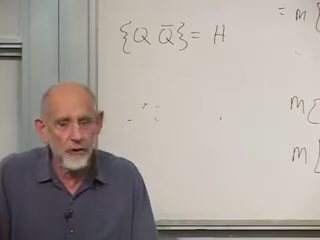
\includegraphics[width=0.62\textwidth]{lecture_05_figure_02.png}
\lectureframe{00:55:46.300}
\caption{La relation de fermeture centrale isolée au tableau. Les accolades et \(Q,\bar Q,H\) sont visibles ; la virgule est implicite dans la notation usuelle de l’anticommutateur.}
\end{figure}

Le zéro de l’énergie a été choisi de sorte que l’état vide ait \(H=0\). Dans l’oscillateur supersymétrique, c’est la convention naturelle : les contributions bosonique et fermionique d’énergie du point zéro se compensent. \editorialnote{Le cours travaille directement avec l’énergie totale au repos et ne fait pas apparaître séparément les termes d’énergie du point zéro ; la convention énoncée explicite ce choix.}

Le Hamiltonien est pair. C’est aussi un générateur de symétrie : il engendre les translations dans le temps. Les générateurs impairs ne se ferment donc pas entre eux sans que l’on inclue le générateur pair des translations temporelles.

\begin{classroomqa}
\audiencequestion{Lequel des éléments de la relation est pair ? Est-ce le Hamiltonien ? \lecturetimestamp{00:58:24}}
\lecturerresponse{Oui. L’énergie est une observable ordinaire, donc \(H\) est pair. La charge supersymétrique \(Q\) est impaire, et le produit de deux quantités impaires est pair ; \(\{Q,\bar Q\}\) peut donc être égal à \(H\). Des générateurs pair et impair sont liés par un commutateur, et non par un anticommutateur.}
\end{classroomqa}

\subsection{Compléter l’algèbre}

Les relations entre éléments de même parité sont immédiates :
\begin{equation}
\{Q,Q\}=2Q^2=0,
\qquad
\{\bar Q,\bar Q\}=2\bar Q^2=0,
\end{equation}
car \(Q^2\) contient \(c_-^2\) et \(\bar Q^2\) contient \(c_+^2\).

Il reste à établir la relation avec \(H\). Posons
\begin{equation}
H\ket{E}=E\ket{E}.
\end{equation}
Si les masses du boson et du fermion sont égales, \(Q\) remplace l’un par l’autre sans changer l’énergie. Par conséquent, \(Q\ket{E}\) est soit nul, soit un autre état propre associé à la même valeur propre :
\begin{equation}
H Q\ket{E}=E Q\ket{E}.
\end{equation}
D’autre part,
\begin{equation}
QH\ket{E}=Q(E\ket{E})=E Q\ket{E}.
\end{equation}
En soustrayant,
\begin{equation}
[H,Q]\ket{E}=0.
\end{equation}
Si les états propres de l’énergie forment une base complète, cette relation vaut comme identité d’opérateurs :
\begin{equation}
[H,Q]=0,
\qquad
[H,\bar Q]=0.
\end{equation}

\begin{classroomqa}
\audiencequestion{Que se passe-t-il si le boson et le fermion n’ont pas la même masse ? \lecturetimestamp{01:01:16}}
\lecturerresponse{Le remplacement de l’un par l’autre change alors l’énergie ; la charge supersymétrique proposée ne commute donc pas avec le Hamiltonien, et la supersymétrie simple disparaît. Pour
\[
H=m_BN_B+m_FN_F,
\]
le résultat explicite est
\[
[H,Q]=(m_B-m_F)Q.
\]
Il s’annule précisément lorsque \(m_B=m_F\). \editorialnote{Le commutateur pour des masses inégales donne directement sous forme d’opérateur l’argument fondé sur le changement d’énergie, et explicite la condition d’égalité des masses.}}
\end{classroomqa}

\begin{classroomqa}
\audiencequestion{Peut-on reprendre plus lentement l’argument fondé sur les états propres de l’énergie ? \lecturetimestamp{01:01:37}}
\lecturerresponse{Partons de \(H\ket{E}=E\ket{E}\). L’égalité des masses implique que \(Q\ket{E}\) possède la même énergie déterminée \(E\), donc \(HQ\ket{E}=EQ\ket{E}\). Dans l’ordre inverse, on obtient \(QH\ket{E}=QE\ket{E}=EQ\ket{E}\), puisque \(E\) est un scalaire ordinaire. La différence s’annule sur chaque état propre de l’énergie. La complétude permet alors d’étendre cette affirmation de ces états à l’équation d’opérateurs \([H,Q]=0\).}
\end{classroomqa}

L’algèbre complète de ce modèle est donc
\begin{align}
\{Q,\bar Q\}&=H,\\
\{Q,Q\}&=\{\bar Q,\bar Q\}=0,\\
[H,Q]&=[H,\bar Q]=0.
\end{align}
Les charges supersymétriques sont des charges impaires conservées. Plus étonnant encore, leur algèbre mêle une opération qui change le type de particule au générateur d’une translation de l’espace-temps.

\section{Pourquoi le Hamiltonien représente une translation temporelle}

Dans ce modèle dépouillé, il n’y a pas de coordonnée spatiale, mais il y a le temps. L’équation de Schrödinger s’écrit
\begin{equation}
i\frac{\partial}{\partial t}\ket{\psi(t)}
=H\ket{\psi(t)}.
\end{equation}

\begin{figure}[H]
\centering
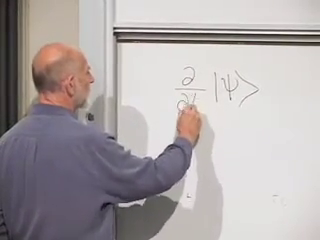
\includegraphics[width=0.56\textwidth]{lecture_05_figure_03.png}
\lectureframe{01:07:26.300}
\caption{La dérivée temporelle écrite à côté de \(\ket{\psi}\). La main masque une partie du dénominateur ; l’équation de Schrödinger complète est donnée ci-dessus.}
\end{figure}

Pour un décalage fini \(\delta\),
\begin{equation}
\ket{\psi(t+\delta)}
=e^{-iH\delta}\ket{\psi(t)}.
\end{equation}
En développant au premier ordre,
\begin{equation}
\ket{\psi(t+\delta)}
=\left(\mathbf 1-i\delta H\right)\ket{\psi(t)}
+O(\delta^2).
\end{equation}
Ainsi, \(H\) est le générateur infinitésimal qui fait évoluer un état dans le temps.

Les symétries internes, comme l’isospin et la couleur, changent également les étiquettes des particules. L’isospin peut mélanger les états du proton et du neutron ; les rotations de couleur mélangent les quarks rouges, verts et bleus. Pourtant, aucune composition de ces transformations internes ne translate un système dans l’espace ou dans le temps. La supersymétrie est différente :
\begin{equation}
\begin{gathered}
\text{odd particle-changing transformation}\\
\mathrel{\stackrel{\{\ ,\ \}}{\Longrightarrow}}\\
\text{time translation}
\end{gathered}
\end{equation}
C’est l’indice que les générateurs impairs pourraient eux-mêmes être des translations, mais selon des coordonnées différentes des coordonnées usuelles.

\section{Le superspace}

\subsection{Une fonction du temps et de coordonnées impaires}

Introduisons une fonction
\begin{equation}
\Psi=\Psi(\theta,\bar\theta,t).
\end{equation}
On peut la considérer comme une fonction d’onde dans le modèle jouet ou, plus généralement, comme un superchamp. Comme le développement impair s’arrête,
\begin{equation}
\Psi(\theta,\bar\theta,t)
=A(t)+\bar\chi(t)\theta
+\bar\theta\chi(t)+F(t)\bar\theta\theta.
\end{equation}
Cet objet unique regroupe des fonctions composantes paires et impaires. \editorialnote{Ce développement en composantes met en œuvre le polynôme de Grassmann présenté plus haut ; il explicite le contenu usuel d’une fonction sur le superspace du modèle.}

Une translation temporelle ordinaire laisse \(\theta,\bar\theta\) fixes et effectue la transformation
\begin{equation}
t\longmapsto t+\delta.
\end{equation}
Au premier ordre,
\begin{equation}
\Psi(\theta,\bar\theta,t+\delta)
=\Psi(\theta,\bar\theta,t)
+\delta\,\partial_t\Psi(\theta,\bar\theta,t).
\end{equation}

\begin{figure}[H]
\centering
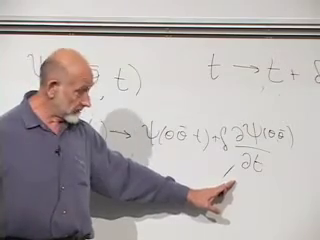
\includegraphics[width=0.72\textwidth]{lecture_05_figure_04.png}
\lectureframe{01:13:15.060}
\caption{Le tableau place \(t\to t+\delta\) au-dessus de la variation au premier ordre de \(\Psi\), en indiquant directement le terme dérivé.}
\end{figure}

\subsection{Translation dans une direction impaire}

Imaginons maintenant une transformation qui décale une coordonnée impaire :
\begin{equation}
\theta\longmapsto\theta+\epsilon,
\end{equation}
où \(\epsilon\) est un autre paramètre de Grassmann impair. Simultanément, faisons subir au temps un déplacement pair nilpotent,
\begin{equation}
t\longmapsto t+i\bar\theta\epsilon.
\end{equation}
\(\bar\theta\) et \(\epsilon\) sont tous deux impairs, si bien que leur produit est pair et peut être ajouté de façon cohérente à la coordonnée paire \(t\).

En plaçant le paramètre à gauche,
\begin{equation}
i\bar\theta\epsilon=-i\epsilon\bar\theta.
\end{equation}
la variation induite est donc
\begin{align}
\delta_\epsilon\Psi
&=\epsilon\,\partial_\theta\Psi
-i\epsilon\bar\theta\,\partial_t\Psi\\
&=\epsilon q_0\Psi,
\end{align}
où
\begin{equation}
q_0=\partial_\theta-i\bar\theta\partial_t.
\end{equation}
Cet opérateur différentiel impair engendre le déplacement combiné. Un générateur conjugué compatible, utilisant des dérivées à gauche, est
\begin{equation}
\bar q_0=-\partial_{\bar\theta}
+i\theta\partial_t.
\end{equation}

Les signes exacts dépendent du choix de dérivées de Grassmann à gauche ou à droite et de la façon dont la conjugaison inverse les facteurs impairs. En revanche, la fermeture sur les translations temporelles doit être indépendante de la convention. Avec les définitions ci-dessus,
\begin{align}
\{q_0,\bar q_0\}
&=i\{\partial_\theta,\theta\}\partial_t
+i\{\bar\theta,\partial_{\bar\theta}\}\partial_t\\
&=2i\partial_t.
\end{align}
Le terme dérivée-dérivée s’annule, de même que le terme quadratique en les coordonnées impaires. Les deux termes mixtes contribuent chacun \(i\partial_t\).

Puisque \(H=i\partial_t\) sur les états dans la représentation de Schrödinger,
\begin{equation}
\{q_0,\bar q_0\}=2H.
\end{equation}
Si nous normalisons les générateurs comme suit :
\begin{equation}
q=\frac{q_0}{\sqrt2},
\qquad
\bar q=\frac{\bar q_0}{\sqrt2},
\end{equation}
alors
\begin{equation}
\boxed{\{q,\bar q\}=H.}
\end{equation}
\editorialnote{Le cours traite délibérément les signes incertains, puis remarque l’apparition d’un facteur deux. La convention affichée, avec des dérivées à gauche, préserve ce calcul fait en classe tout en fixant une normalisation cohérente. D’autres conventions usuelles déplacent les signes entre les décalages des coordonnées et les générateurs.}

\begin{classroomqa}
\audiencequestion{D’où vient le facteur deux final dans l’anticommutateur du superspace ? \lecturetimestamp{01:24:21}}
\lecturerresponse{Il y a deux contributions mixtes égales. L’une vient de \(\{\partial_\theta,\theta\}=1\), l’autre de \(\{\partial_{\bar\theta},\bar\theta\}=1\). Chacune multiplie la dérivée temporelle. Les générateurs non normalisés donnent donc \(2i\partial_t\) ; un facteur \(1/\sqrt2\) dans chaque charge supersymétrique rétablit la normalisation précédente.}
\end{classroomqa}

\begin{classroomqa}
\audiencequestion{La construction repose-t-elle sur l’hypothèse que \(\epsilon\) est petit ? \lecturetimestamp{01:24:51}}
\lecturerresponse{Elle repose sur la nilpotence, non sur une grandeur numérique ordinaire. Puisque \(\epsilon^2=0\), tout développement en un seul \(\epsilon\) s’arrête après le premier ordre. Le qualifier d’infinitésimal ou de petit est une analogie utile, mais la troncature est exacte.}
\end{classroomqa}

\editorialnote{Les paramètres de Grassmann n’ont pas de grandeur positive ordinaire. Leur rôle de paramètres infinitésimaux découle de la nilpotence et de l’arrêt exact du développement.}

\subsection{Signification géométrique}

L’algèbre possède maintenant deux réalisations équivalentes. Dans la représentation par oscillateurs, \(Q\) et \(\bar Q\) remplacent les fermions par des bosons et les bosons par des fermions. Dans la représentation géométrique, \(q\) et \(\bar q\) translatent une fonction selon des directions impaires tout en induisant un décalage temporel ordinaire. Dans les deux représentations,
\begin{equation}
\begin{gathered}
\{\text{supercharge},\text{conjugate supercharge}\}\\
=\text{time-translation generator}.
\end{gathered}
\end{equation}

L’espace des coordonnées généralisées qui contient \(t,\theta,\bar\theta\) est le superspace. Dans une théorie relativiste des champs, il contient aussi les coordonnées spatiales ordinaires, et les charges supersymétriques se ferment sur la quantité de mouvement complète de l’espace-temps \(P_\mu\), et pas uniquement sur \(H=P_0\). Courber cette structure conduit vers la supergravité.

D’un certain point de vue, les variables de Grassmann sont un outil efficace pour organiser les bosons et les fermions. D’un autre, la relation de fermeture exprime une idée bien plus profonde : la distinction entre le type de particule et la géométrie de l’espace-temps n’est plus absolue. Deux déplacements dans des directions impaires produisent un déplacement selon une direction ordinaire. La question de savoir si la nature réalise cette structure expérimentalement est distincte du fait mathématique que cette structure est cohérente, économique et remarquablement rigide.

\chapter{Pourquoi la supersymétrie pourrait avoir de l’importance}

\lectureoverview{Les fluctuations du vide relient les sujets de ce chapitre.
Les conditions aux limites produisent la force de Casimir, les effets de boucle menacent la masse du Higgs, de nouvelles particules virtuelles modifient l’évolution des couplages de jauge et l’énergie du vide gouverne l’expansion cosmique. Ces problèmes motivent la supersymétrie à basse énergie, qui pourrait stabiliser l’échelle du Higgs, fournir un candidat à la matière noire et améliorer l’unification des couplages de jauge. Nous construisons ensuite des superchamps à l’aide de coordonnées de Grassmann et utilisons l’intégration de Berezin pour extraire une action supersymétrique.}

\section{Fluctuations du vide entre des plaques réfléchissantes}

Nous revenons à la supersymétrie en commençant par répondre à une question sur l’effet Casimir. Plaçons deux plaques réfléchissantes parallèles séparées par une distance \(d\). Même en l’absence de particules réelles, un champ quantique présente des fluctuations du vide. On peut les représenter comme des processus virtuels ou, de manière équivalente, comme le mouvement de point zéro des modes oscillatoires du champ. Les plaques imposent des conditions aux limites : les fluctuations autorisées entre elles diffèrent donc de celles de l’espace sans restriction.

La grandeur importante n’est pas une valeur absolue de l’énergie zéro, mais la variation produite par un changement de la séparation. Notons \(\mathcal E(d)=E(d)/A\) l’énergie du vide par unité de surface. Dès que \(\mathcal E\) dépend de \(d\), il s’agit d’une énergie potentielle, et la force par unité de surface vaut
\begin{equation}
\frac{F}{A}=-\frac{d\mathcal E}{dd}.
\end{equation}
Ainsi, un réarrangement des processus virtuels devient une force observable. Dans l’exemple électromagnétique classique de plaques parfaitement conductrices, l’énergie et la pression sont
\begin{align}
\mathcal E(d)&=-\frac{\pi^2}{720\,d^3},\\
\frac{F}{A}&=-\frac{\pi^2}{240\,d^4},
\end{align}
dans les unités \(\hbar=c=1\).\editorialnote{Ces coefficients et la distinction entre l’énergie par unité de surface en \(d^{-3}\) et la pression en \(d^{-4}\) répondent à la question de dimension soulevée au tableau. Il s’agit du résultat standard pour des plaques idéales, et non d’une démonstration présentée ici.}Le signe moins indique une attraction.

\begin{classroomqa}
\audiencequestion{La puissance quatrième décrit-elle la force ou l’énergie ? \lecturetimestamp{00:04:39}}
\lecturerresponse{Pour des plaques parallèles dans un espace-temps à quatre dimensions, l’énergie par unité de surface décroît comme \(d^{-3}\), tandis que la dérivation par rapport à \(d\) donne une force par unité de surface qui décroît comme \(d^{-4}\). L’analyse dimensionnelle fixe déjà ces puissances une fois que l’on rétablit \(\hbar\) et \(c\).}
\end{classroomqa}

On résume parfois le calcul en disant que les plaques interrompent les boucles de photons virtuels. Cette représentation est utile à condition de ne pas la prendre trop littéralement. Le calcul précis consiste en une modification du spectre des modes du champ autorisés ou, de manière équivalente, de l’action effective quantique. Ces deux formulations conduisent à la même énergie dépendant de la séparation.

\begin{classroomqa}
\audiencequestion{La force de Casimir peut-elle être répulsive plutôt qu’attractive ? \lecturetimestamp{00:07:48}}
\lecturerresponse{Oui. Le signe n’est pas universel : il dépend des champs, de la géométrie, des matériaux et des conditions aux limites. Les boucles fermioniques ont souvent un signe opposé à celui des boucles bosoniques, ce qui motive la suggestion faite au tableau ; toutefois, la statistique fermionique ne constitue pas à elle seule un théorème général selon lequel toute force de Casimir serait répulsive.\editorialnote{Cette réserve remplace une réponse de cours délibérément hésitante par l’énoncé général nécessaire pour éviter une fausse règle universelle.}}
\end{classroomqa}

\subsection{Qu’est-ce qui constituerait une preuve de l’énergie du vide ?}

La force de Casimir est mesurée, et les observables atomiques sont également sensibles aux boucles du vide. Pourtant, aucun de ces faits ne démontre à lui seul qu’une énergie absolue du vide gravite. Une expérience de Casimir mesure une différence d’énergie due aux conditions aux limites ; on peut décrire la même force sans attribuer de sens opérationnel à une somme de point zéro absolue et non bornée.

Le test décisif vient de la gravité. L’énergie est une charge gravitationnelle. Si le vide porte une densité d’énergie uniforme, celle-ci doit entrer dans les équations d’Einstein et influer sur l’expansion cosmique. L’expansion accélérée de l’Univers constitue donc la preuve gravitationnelle directe d’une composante apparentée au vide.

\begin{classroomqa}
\audiencequestion{Pourquoi les ouvrages de vulgarisation qualifient-ils l’énergie du vide de mystérieuse, comme si les physiciens ne savaient pas ce que c’est ? \lecturetimestamp{00:08:19}}
\lecturerresponse{La théorie quantique des champs attribue une contribution de point zéro à chaque champ ; la possibilité d’une énergie du vide n’a donc rien de mystérieux. Le mystère est quantitatif : pourquoi la valeur gravitationnelle est-elle extraordinairement faible par rapport aux estimations fondées sur les champs quantiques connus et une coupure à haute énergie ? Le fait surprenant est son absence presque totale, et non sa simple existence.}
\end{classroomqa}

Pendant de nombreuses années, la borne supérieure observationnelle était si faible qu’il était psychologiquement tentant de poser la constante cosmologique exactement égale à zéro et de chercher un principe imposant cette annulation. Des observations cosmologiques plus précises ont plutôt révélé une petite valeur non nulle. Cette découverte n’a pas rendu l’énergie du vide étrangère sur le plan conceptuel ; elle a rendu impossible d’ignorer le degré de suppression inexpliqué. La comparaison pertinente dépend de l’échelle ultraviolette supposée, mais toute estimation naturelle à haute énergie exige une annulation considérable.

\section{Action d’une charge supersymétrique sur un état à plusieurs particules}

Avant d’énumérer les raisons de croire à la supersymétrie, dissipons un paradoxe possible. Un nombre arbitrairement grand de bosons peut occuper un même mode, tandis qu’un mode fermionique a un nombre d’occupation égal à zéro ou à un. Si une symétrie échange les bosons et les fermions, transforme-t-elle mille bosons dans un même mode en mille fermions interdits ?

Non. Un générateur fermionique modifie l’état quantique d’un quantum à la fois. Dans le modèle de l’oscillateur, notons \(a\) l’opérateur qui annihile un boson et \(c^\dagger\) celui qui crée son partenaire fermionique. On peut représenter une charge supersymétrique par
\begin{equation}
Q=c^\dagger a.
\end{equation}
Sur un état contenant \(n\) bosons et aucun fermion,
\begin{equation}
Q\ket{n,0}
=\sqrt n\,\ket{n-1,1}.
\end{equation}
Un boson a été supprimé et un fermion a été ajouté. Une nouvelle action de la même charge donne zéro :
\begin{equation}
Q^2=(c^\dagger)^2a^2=0.
\end{equation}
C’est la nilpotence héritée des opérateurs de création fermioniques.

\begin{classroomqa}
\audiencequestion{Si de nombreux bosons occupent le même état, pourquoi une transformation supersymétrique ne produit-elle pas de nombreux fermions dans ce même état, en violation du principe d’exclusion ? \lecturetimestamp{00:12:05}}
\lecturerresponse{Le générateur ne remplace pas toute la population. Il modifie l’état d’une unité de nombre fermionique. On ne peut pas composer la même charge fermionique comme un générateur de rotation ordinaire, car son carré s’annule. Une charge complémentaire peut inverser l’échange, et l’anticommutateur mixte se referme sur la translation temporelle.}
\end{classroomqa}

La dernière phrase est essentielle. L’abréviation \(Q^2=0\) s’applique à une composante chirale individuelle ou à la charge simple que nous venons d’écrire ; elle ne signifie pas que tout produit de charges supersymétriques s’annule. En supersymétrie à quatre dimensions,
\begin{equation}
\{Q_\alpha,\bar Q_{\dot\beta}\}
=2\sigma^\mu_{\alpha\dot\beta}P_\mu,
\end{equation}
alors que
\begin{equation}
\{Q_\alpha,Q_\beta\}=0,
\qquad
\{\bar Q_{\dot\alpha},\bar Q_{\dot\beta}\}=0
\end{equation}
pour l’algèbre minimale sans charges centrales.\editorialnote{Cette forme en composantes précise l’abréviation utilisée en cours : l’action répétée de la même \(Q\) s’annule, tandis qu’une charge supersymétrique et sa conjuguée engendrent une translation.}

\section{Trois raisons de rechercher la supersymétrie à basse énergie}

\begin{classroomqa}
\audiencequestion{Existe-t-il d’autres motivations pour la supersymétrie que l’annulation de l’énergie du vide ? \lecturetimestamp{00:15:06}}
\lecturerresponse{Trois motivations étroitement liées se dégagent : le contrôle de l’auto-énergie du Higgs, un éventuel candidat stable à la matière noire et une convergence beaucoup plus précise des couplages de jauge à haute énergie. Aucune ne prouve que la supersymétrie se réalise dans la nature, mais ensemble, elles en font une théorie sérieuse à mettre à l’épreuve.}
\end{classroomqa}

L’expression \emph{supersymétrie à basse énergie} est relative. Elle ne signifie pas que les partenaires supersymétriques sont légers à l’échelle quotidienne ; elle signifie que leurs masses ne sont pas très supérieures aux échelles électrofaible et des accélérateurs. Les trois arguments s’affaiblissent si les masses des partenaires supersymétriques sont poussées arbitrairement haut.

\subsection{Protéger l’échelle du Higgs}

La masse d’un scalaire est exceptionnellement sensible à la physique des hautes énergies. Schématiquement, une boucle bosonique produit une correction de la forme
\begin{equation}
\delta m_H^2\big|_{\mathrm B}
\sim +\frac{\lambda}{16\pi^2}\Lambda^2,
\end{equation}
où \(\Lambda\) désigne l’échelle jusqu’à laquelle on utilise la théorie effective. Une boucle fermionique porte le signe opposé,
\begin{equation}
\delta m_H^2\big|_{\mathrm F}
\sim -\frac{|y|^2}{8\pi^2}\Lambda^2.
\end{equation}
Les coefficients dépendent de l’interaction et des multiplicités des champs, mais la supersymétrie établit entre eux des relations qui annulent la sensibilité ultraviolette dominante entre partenaires.\editorialnote{Ces formules schématiques de boucle exposent le fondement mathématique de l’argument qualitatif sur l’auto-énergie. Elles ne sont pas destinées à constituer un calcul complet de la masse du Higgs du Modèle standard.}

Cela importe, car la valeur moyenne du champ de Higgs fixe l’échelle électrofaible. Les masses des bosons de jauge et des fermions vérifient des relations telles que
\begin{equation}
m_W=\frac{gv}{2},
\qquad
m_f=\frac{y_fv}{\sqrt2}.
\end{equation}
Si le secteur de Higgs était naturellement entraîné vers une échelle immense, le spectre familier des particules à basse énergie disparaîtrait, à moins d’ajuster les paramètres nus avec une précision extrême pour compenser les corrections radiatives.

Une supersymétrie exacte rendrait l’annulation exacte, mais la supersymétrie exacte est déjà exclue par les masses inégales des bosons et fermions observés. Avec une supersymétrie brisée doucement, la sensibilité quadratique est remplacée par une dépendance aux écarts de masse entre partenaires, schématiquement
\begin{equation}
\delta m_H^2
\sim
\frac{g^2}{16\pi^2}
\left(m_{\mathrm{soft}}^2-m_{\mathrm{ordinary}}^2\right)
\ln\frac{\Lambda^2}{m_{\mathrm{soft}}^2}.
\end{equation}
L’annulation ne reste utile que si l’écart n’est pas trop grand.

\subsection{Un état final stable pour les cascades de désintégration de la matière noire}

Séparons le spectre en particules ordinaires et en leurs partenaires supersymétriques. Un fermion a un partenaire bosonique ; un boson a un partenaire fermionique. Si les interactions conservent une parité qui distingue ces deux classes, toute désintégration d’un partenaire supersymétrique doit en laisser un autre :
\begin{equation}
\widetilde X
\longrightarrow X+\widetilde Y
\longrightarrow X+Y+\widetilde Z
\longrightarrow\cdots.
\end{equation}
La cascade ne peut pas éliminer son dernier partenaire supersymétrique. Elle se termine donc par la particule supersymétrique la plus légère, le LSP.

La symétrie couramment utilisée est la parité \(R\),
\begin{equation}
R_p=(-1)^{3(B-L)+2s}.
\end{equation}
Les particules du Modèle standard ont \(R_p=+1\), tandis que leurs partenaires supersymétriques ont \(R_p=-1\). Si \(R_p\) est exacte, chaque interaction comporte un nombre pair de partenaires supersymétriques et le LSP est stable.\editorialnote{La supersymétrie seule ne garantit pas la stabilité du LSP. Cette stabilité exige la conservation de la parité \(R\) ou d’une autre symétrie ayant la même conséquence ; sans elle, le LSP peut se désintégrer.}

La matière noire doit survivre au moins pendant des durées cosmologiques. Elle doit aussi interagir assez faiblement pour traverser à plusieurs reprises le disque galactique visible sans perdre une quantité importante d’énergie. Une population chargée électriquement ou soumise à l’interaction forte diffuserait, dissiperait de l’énergie et tendrait à s’effondrer vers la même structure mince que la matière ordinaire. Le halo étendu observé indique plutôt une composante neutre et faiblement interactive.

Cela ne permet pas d’identifier le LSP de façon unique. Selon le modèle et le schéma de brisure de symétrie, le candidat pourrait être un mélange neutre de jauginos électrofaibles et de higgsinos, ou bien un gravitino. Les candidats chargés ou colorés sont soumis à de fortes contraintes. La supersymétrie ne fournit pas une réponse garantie, mais un mécanisme naturel qui produit un état final neutre et à longue durée de vie.

\section{Couplages qui évoluent et indice d’unification}

La troisième motivation part de l’écrantage des charges. La valeur mesurée d’un couplage dépend de l’échelle d’énergie, car des particules virtuelles habillent l’interaction. En électromagnétisme, une boucle électron-positron insérée dans un propagateur de photon écrante la charge à grande distance. À plus courte distance, ou pour un transfert d’impulsion plus élevé, une moindre partie de ce nuage de polarisation se trouve entre les sondes ; la charge effective est donc plus grande.

Posons
\begin{equation}
\alpha_i=\frac{g_i^2}{4\pi}.
\end{equation}
À une boucle, l’inverse du couplage évolue linéairement avec le logarithme de l’énergie :
\begin{equation}
\frac{d\alpha_i^{-1}}{d\ln\mu}
=-\frac{b_i}{2\pi}.
\end{equation}
Ainsi,
\begin{equation}
\alpha_i^{-1}(\mu)
=\alpha_i^{-1}(\mu_0)
-\frac{b_i}{2\pi}\ln\frac{\mu}{\mu_0}.
\end{equation}
\editorialnote{Cette équation à une boucle donne la formulation précise des droites presque rectilignes tracées en fonction du logarithme de l’énergie. Les seuils et les corrections d’ordre supérieur courbent légèrement ces droites.}

Au-dessus de l’échelle électrofaible, les trois couplages de jauge fondamentaux sont ceux de
\begin{equation}
U(1)_Y,\qquad SU(2)_L,\qquad SU(3)_c.
\end{equation}
Le couplage électromagnétique utilisé comme repère à basse énergie est une combinaison des deux premiers après la brisure de la symétrie électrofaible. Pour la QCD, les champs de jauge non abéliens produisent un anti-écrantage : le couplage fort diminue à courte distance, phénomène appelé liberté asymptotique. Par conséquent, \(\alpha_3^{-1}\) augmente avec \(\ln\mu\), tandis que les inverses des autres couplages ont des pentes différentes.

Les courbes du Modèle standard semblent se rapprocher, mais elles ne se rencontrent pas en un même point. Les partenaires supersymétriques modifient les boucles virtuelles et donc les coefficients \(b_i\). Avec la normalisation conventionnelle de grande unification,
\begin{align}
(b_1,b_2,b_3)_{\mathrm{SM}}
&=\left(\frac{41}{10},-\frac{19}{6},-7\right),\\
(b_1,b_2,b_3)_{\mathrm{MSSM}}
&=\left(\frac{33}{5},1,-3\right).
\end{align}
les courbes extrapolées de la théorie supersymétrique se rencontrent avec une bien meilleure précision, près de
\begin{equation}
M_{\mathrm{GUT}}\sim 10^{16}\ \mathrm{GeV}.
\end{equation}
Aucune expérience n’atteint directement cette échelle. On mesure les couplages à basse énergie, le contenu en champs détermine leur évolution, puis on extrapole les courbes sur de nombreux ordres de grandeur. Deux droites se croisent toujours quelque part ; le fait non trivial est que trois droites indépendantes se rencontrent à proximité d’un même point.

\begin{classroomqa}
\audiencequestion{L’extrapolation améliorée suppose-t-elle une supersymétrie exacte et des masses identiques pour les partenaires ? \lecturetimestamp{00:38:09}}
\lecturerresponse{Non. La supersymétrie est brisée, et les masses sont donc différentes. Ce qui importe, c’est le moment où les boucles des partenaires supersymétriques entrent en jeu dans l’évolution. Si les partenaires ne sont pas trop lourds, les pentes changent assez tôt pour que les trois couplages convergent. S’ils sont extrêmement lourds, les seuils supersymétriques apparaissent trop tard et la convergence améliorée disparaît.}
\end{classroomqa}

Les corrections de seuil et le spectre inconnu à haute énergie empêchent d’affirmer littéralement que les trois droites se rencontrent avec une exactitude mathématique. Le résultat reste néanmoins frappant : la même échelle approximative des partenaires supersymétriques qui aide à stabiliser le Higgs et fournit un candidat thermique à la matière noire améliore aussi l’unification.

\subsection{Gravité et échelle commune de haute énergie}

La gravité se comporte différemment, car sa charge est l’énergie elle-même. Une mesure sans dimension utile à l’énergie du centre de masse \(E\) est
\begin{equation}
\alpha_G(E)\sim GE^2
=\left(\frac{E}{M_{\mathrm{Pl}}}\right)^2.
\end{equation}
Aux énergies ordinaires, cette quantité est extraordinairement petite, mais elle croît comme le carré de \(E\). Son inverse diminue donc bien plus rapidement que les inverses des couplages de jauge, qui évoluent de façon logarithmique, et devient de l’ordre de l’unité près de l’échelle de Planck.

Cette comparaison suggère que toutes les interactions pourraient être gouvernées par des échelles élevées voisines, mais elle est moins nette que l’unification des couplages de jauge. Les couplages de jauge sont des paramètres sans dimension dans les théories des champs renormalisables ; la constante de Newton a une dimension, si bien que représenter la gravité sur le même graphique exige une convention.

\begin{classroomqa}
\audiencequestion{Les partenaires supersymétriques participent-ils aux trois mêmes interactions de jauge ou définissent-ils de nouvelles forces ? \lecturetimestamp{00:42:35}}
\lecturerresponse{Ils portent les mêmes nombres quantiques de jauge que leurs partenaires. Un sélectron a la charge électrique de l’électron, et un squark possède les charges de couleur et électrofaibles correspondantes à celles du quark, même si leurs spins et leurs masses diffèrent. Leurs boucles modifient donc les mêmes interactions de jauge au lieu d’en introduire trois nouvelles.}
\end{classroomqa}

\begin{classroomqa}
\audiencequestion{La découverte d’un partenaire supersymétrique au LHC constituerait-elle une preuve définitive de la supersymétrie ? \lecturetimestamp{00:43:27}}
\lecturerresponse{Une particule inhabituelle ne suffirait pas à elle seule, quel que soit le nom qu’on lui donne ; en revanche, un spectre de partenaires supersymétriques qui respecterait les relations de supersymétrie entre spins, charges, masses et couplages serait très caractéristique. La supersymétrie impose de nombreuses contraintes corrélées : le schéma détaillé des interactions constituerait donc le test décisif.}
\end{classroomqa}

\subsection{Pourquoi déplacer l’échelle a un coût}

Si les partenaires supersymétriques se trouvent juste au-delà des limites expérimentales, les trois motivations peuvent encore s’appliquer. Si leurs masses augmentent de plusieurs ordres de grandeur, chacun des arguments s’affaiblit :
\begin{enumerate}
\item Les annulations de la masse du Higgs laissent une forte sensibilité résiduelle à l’écart de masse.
\item Un reliquat thermique conventionnel à l’échelle électrofaible n’apparaît plus à l’échelle attendue.
\item Les seuils liés à l’évolution des couplages se déplacent vers les hautes énergies, et les trois couplages se rencontrent avec moins de précision.
\end{enumerate}
La supersymétrie pourrait toujours exister à une échelle beaucoup plus élevée, mais elle ne résoudrait plus ces problèmes particuliers de basse énergie avec la même économie. La longévité de cette idée ne prouve pas que la nature doit l’adopter ; elle montre que la proposition est suffisamment cohérente pour mériter un test décisif.

\section{Ce que la cosmologie peut et ne peut pas nous apprendre sur la matière noire}

\begin{classroomqa}
\audiencequestion{La cosmologie standard peut-elle déterminer la quantité de matière noire et la masse de chaque particule de matière noire, comme la nucléosynthèse impose des contraintes sur l’hydrogène et l’hélium ? \lecturetimestamp{00:46:32}}
\lecturerresponse{La cosmologie mesure très bien la densité totale de masse de matière noire, mais cette densité ne permet pas à elle seule de distinguer la masse du nombre de particules. Une même densité peut être portée par quelques particules lourdes ou par un nombre immense de particules très légères. Il faut une théorie supplémentaire ou des observations non gravitationnelles pour identifier la particule microscopique.}
\end{classroomqa}

Deux grandes possibilités illustrent cette ambiguïté. Une particule faiblement interactive, proche de l’échelle électrofaible ou du TeV, peut se découpler du bain thermique chaud. À l’autre extrême, un boson extrêmement léger comme l’axion peut occuper une configuration cohérente de champ ou un condensat. Le fait que les deux mécanismes les mieux développés se situent près des extrêmes opposés n’interdit pas les possibilités intermédiaires.

La structure du halo impose elle-même une contrainte importante. La matière noire traverse la matière ordinaire avec peu de frottement et reste donc étendue dans l’espace au lieu de s’effondrer en un disque lumineux. Les courbes de rotation et d’autres phénomènes gravitationnels nous indiquent que cette masse est présente, mais ne permettent pas à eux seuls de dénombrer les particules.

\begin{classroomqa}
\audiencequestion{L’Univers primordial aurait-il pu ne contenir au départ que des superparticules, qui se seraient ensuite désintégrées en particules que nous observons ? \lecturetimestamp{00:49:11}}
\lecturerresponse{À des températures très supérieures à toutes les masses pertinentes, les réactions rapides conduisent les espèces vers l’équilibre thermique plutôt que vers une population initiale arbitraire constituée d’une seule sorte de particules. Les collisions ordinaires créent des partenaires supersymétriques lorsqu’ils sont sous-abondants, tandis que les collisions et désintégrations de partenaires supersymétriques réalimentent la population de particules ordinaires. L’abondance précise dépend des interactions et des degrés de liberté, mais le plasma chaud tend continuellement vers l’équilibre.}
\end{classroomqa}

À mesure que l’Univers se refroidit, les espèces massives voient leur abondance supprimée par le facteur de Boltzmann et s’annihilent ou se désintègrent. Un LSP stable cesse de suivre l’équilibre lorsque son taux d’interaction devient inférieur au taux d’expansion cosmique :
\begin{equation}
\Gamma_{\mathrm{ann}}
\sim n\langle\sigma v\rangle
\lesssim H.
\end{equation}
Les particules restantes constituent une abondance relique.\editorialnote{Ce critère de découplage donne la formulation quantitative standard qui complète l’argument de l’équilibre thermique. D’autres candidats au rôle de LSP, notamment les gravitinos à couplage très faible, peuvent avoir une histoire non thermique.}

\begin{classroomqa}
\audiencequestion{De quelle particule ordinaire le LSP est-il le partenaire, et doit-il être non interactif ? \lecturetimestamp{00:51:05}}
\lecturerresponse{Il n’existe pas de réponse indépendante du modèle. On s’attend à ce qu’un LSP viable comme matière noire soit électriquement neutre et incolore, mais il n’a pas besoin d’être complètement non interactif. Il peut être un mélange apparenté au photon, aux bosons de jauge faibles et aux champs de Higgs, ou bien être le gravitino. Son identité précise découle du spectre de brisure de la supersymétrie.}
\end{classroomqa}

\section{Diagrammes du vide, diagrammes d’auto-énergie et expansion}

\begin{classroomqa}
\audiencequestion{Quelle différence y a-t-il entre la divergence du Higgs et celle de l’énergie du vide ? \lecturetimestamp{00:52:09}}
\lecturerresponse{Un diagramme du vide ne comporte aucune ligne de particule externe ; il modifie l’action effective du vide et contribue à son énergie. Un diagramme d’auto-énergie du Higgs comporte deux jambes externes de Higgs ; il modifie le propagateur du Higgs et donc sa masse. Les deux mettent en jeu des fluctuations virtuelles, mais répondent à des questions différentes.}
\end{classroomqa}

On peut se représenter une particule réelle comme une impureté insérée dans le vide. Les fluctuations du vide qui se couplent à cette impureté modifient sa propagation et sa masse. Les plaques de Casimir modifient elles aussi les fluctuations du vide, mais par l’intermédiaire de conditions aux limites macroscopiques. Dans les deux cas, les fluctuations quantiques réagissent à ce qui a été introduit ; c’est l’observable corrigée qui diffère.

\vspace{-2pt}\subsection{La matière, le rayonnement et l’énergie du vide se diluent différemment}

Soit \(a(t)\) le facteur d’échelle cosmologique, et
\begin{equation}
H=\frac{\dot a}{a}
\end{equation}
le paramètre de Hubble. La conservation locale du tenseur énergie-impulsion dans un Univers homogène donne
\begin{equation}
\dot\rho+3H(\rho+p)=0.
\end{equation}
Pour une équation d’état \(p=w\rho\), on obtient par intégration
\begin{equation}
\rho(a)\propto a^{-3(1+w)}.
\end{equation}
\editorialnote{L’équation de continuité fournit la dérivation concise qui sous-tend les explications fondées sur le dénombrement des particules et l’étirement des longueurs d’onde.}

Pour la matière froide non relativiste, \(p\approx0\), donc
\begin{equation}
\rho_m\propto a^{-3}.
\end{equation}
Un volume comobile fixé croît comme \(a^3\), tandis que l’énergie de masse de ses particules reste approximativement constante.

Pour le rayonnement, \(p=\rho/3\), et
\begin{equation}
\rho_r\propto a^{-4}.
\end{equation}
Trois puissances proviennent de la dilution de la densité numérique. La quatrième est due au décalage vers le rouge :
\begin{equation}
\lambda\propto a,
\qquad
E_\gamma=\frac{2\pi\hbar c}{\lambda}\propto a^{-1}.
\end{equation}

\begin{classroomqa}
\audiencequestion{Si le photon possède une fonction d’onde, pourquoi peut-on le considérer comme une particule plutôt que comme une onde pour dériver la loi de dilution ? \lecturetimestamp{00:58:21}}
\lecturerresponse{Cette distinction ne change pas la loi d’échelle. Dans la description en termes de particules, le nombre de quanta dans un volume comobile est fixé et l’énergie de chaque quantum subit un décalage vers le rouge en \(a^{-1}\). Dans la description classique en termes d’ondes, la longueur d’onde s’étire et l’énergie du champ diminue de la même quantité. On peut employer la formulation qui rend l’expansion la plus facile à comprendre.}
\end{classroomqa}

L’énergie du vide vérifie \(p_\Lambda=-\rho_\Lambda\), donc
\begin{equation}
\rho_\Lambda=\text{constant}.
\end{equation}
Elle ne se dilue pas lorsque l’espace se dilate. En effet, une région comobile contient
\begin{equation}
E_\Lambda=\rho_\Lambda a^3V_0,
\end{equation}
ce qui augmente avec son volume physique. C’est ce fait qui soulève la question de la conservation de l’énergie, que nous aborderons bientôt.

Ces différentes puissances structurent l’histoire cosmique. Le rayonnement décroît le plus vite, la matière décroît plus lentement, et l’énergie du vide ne décroît pas du tout. Une faible contribution du vide peut donc être négligeable dans l’Univers primordial et dominer à une époque tardive. Selon les valeurs approximatives évoquées ici, le budget énergétique actuel comprend environ \(70\%\) d’énergie du vide et \(30\%\) de matière, le rayonnement étant bien moindre.

\section{La géométrie égale l’énergie}

La composante temporelle-temporelle des équations d’Einstein transforme les lois d’échelle précédentes en dynamique. Le tableau commence par un slogan et un seul terme géométrique.

\begin{figure}[H]\centering
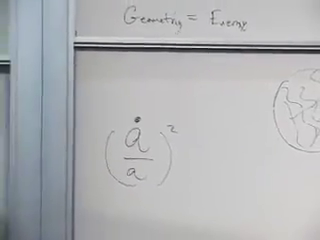
\includegraphics[width=0.68\textwidth]{lecture_06_figure_03.png}\lectureframe{01:06:37.088}\caption{\emph{La géométrie égale l’énergie}, avec le terme d’expansion \(H^2=(\dot a/a)^2\) inscrit en dessous.}\end{figure}

Pour un Univers homogène et isotrope, la première équation de Friedmann est
\begin{equation}
H^2+\frac{k}{a^2}
=\frac{8\pi G}{3}\rho,
\end{equation}
dans les unités \(c=1\), où \(k=+1,0,-1\) désigne une géométrie spatiale fermée, plate ou ouverte, et
\begin{equation}
\rho
=\rho_{\mathrm{ordinary}}
+\rho_{\mathrm{dark}}
+\rho_{\mathrm{radiation}}
+\rho_{\mathrm{vacuum}}.
\end{equation}
Le signe apparaissant à côté de \(1/a^2\) dépend du fait que le terme de courbure soit laissé à gauche ou déplacé à droite, ainsi que de la valeur de \(k\).

\begin{figure}[H]\centering
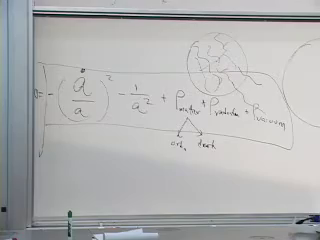
\includegraphics[width=0.96\textwidth]{lecture_06_figure_04.png}\lectureframe{01:08:46.794}\caption{Le bilan complet au tableau : l’expansion et la courbure spatiale du côté géométrique, la matière, le rayonnement et l’énergie du vide du côté des sources. La matière est en outre séparée en composantes ordinaire et noire.}\end{figure}

\subsection{La contrainte hamiltonienne cosmologique}

\begin{classroomqa}
\audiencequestion{Si l’énergie du vide dans une région comobile augmente avec l’expansion de l’Univers, existe-t-il une densité d’énergie nette constante ou une énergie totale conservée ? \lecturetimestamp{01:01:51}}
\lecturerresponse{La relativité générale ne fournit pas d’énergie globale universelle pour un espace-temps en expansion arbitraire. Toutefois, dans la réduction cosmologique homogène, l’équation d’Einstein temporelle-temporelle est une contrainte hamiltonienne. Lorsque la géométrie et la matière sont placées du même côté, le hamiltonien soumis à cette contrainte s’annule. Les termes de matière qui varient sont compensés par les degrés de liberté gravitationnels, plutôt que par une énergie ordinaire fixe dans une boîte.}
\end{classroomqa}

Schématiquement, l’énoncé canonique est
\begin{equation}
\mathcal H_{\mathrm{gravity}}
+\mathcal H_{\mathrm{matter}}
=0.
\end{equation}
C’est là le sens précis de l’affirmation selon laquelle l’énergie totale est nulle. Il s’agit d’une équation du mouvement imposée par l’invariance par reparamétrisation du temps, et non de l’affirmation que chaque densité d’énergie locale s’annule. Dans un volume comobile, l’énergie de la matière ordinaire reste à peu près constante, celle du rayonnement diminue et l’énergie du vide augmente ; dans le même temps, la contribution gravitationnelle et le taux d’expansion s’ajustent de sorte que la contrainte d’Einstein reste satisfaite.

La conservation locale reste exacte :
\begin{equation}
\nabla_\mu T^{\mu\nu}=0.
\end{equation}
Pour le fluide homogène, il s’agit précisément de l’équation de continuité
\(\dot\rho+3H(\rho+p)=0\). Ce qui échoue en général, c’est l’intuition issue de l’espace-temps plat selon laquelle il devrait aussi exister une somme globale de l’énergie de la matière, indépendante des coordonnées et conservée dans un univers en expansion.\editorialnote{Cette distinction précise l’affirmation pédagogique selon laquelle l’énergie est toujours nulle : la conservation covariante locale et la contrainte hamiltonienne cosmologique sont exactes, tandis qu’une énergie globale unique de la matière et de la gravitation n’est généralement pas définie.}

\begin{classroomqa}\audiencequestion{La contrainte nulle est-elle la condition qui détermine si l’Univers est ouvert, fermé ou plat ? \lecturetimestamp{01:04:42}}\lecturerresponse{Non. La contrainte hamiltonienne s’applique dans tous les cas. Les univers ouvert, plat et fermé se distinguent par l’indice de courbure \(k\) et donc par le terme \(k/a^2\). La courbure modifie une contribution au bilan ; elle n’active ni ne désactive la contrainte.}\end{classroomqa}

\section{Coordonnées de Grassmann et superchamps}

\begin{classroomqa}\audiencequestion{Les nombres de Grassmann apparaissent-ils réellement dans le lagrangien de la théorie ? \lecturetimestamp{01:09:37}}\lecturerresponse{Ils apparaissent d’abord parce que les champs fermioniques sont impairs au sens de Grassmann. Ils apparaissent une seconde fois comme coordonnées de l’espace supersymétrique. Les superchamps dépendent de ces coordonnées impaires, et les actions supersymétriques se construisent en dérivant par rapport à celles-ci et en intégrant sur celles-ci.}\end{classroomqa}

Un champ ordinaire est une fonction de l’espace-temps,
\begin{equation}
\phi=\phi(x^\mu).
\end{equation}
La supersymétrie minimale en quatre dimensions augmente \(x^\mu\) de deux composantes de spineur impair \(\theta^\alpha\) et de leur conjugué \(\bar\theta^{\dot\alpha}\) :
\begin{equation}
z^M=(x^\mu,\theta^\alpha,\bar\theta^{\dot\alpha}).
\end{equation}
Il y a deux composantes complexes impaires, soit quatre directions réelles impaires. Un superchamp est une fonction définie sur cet espace supersymétrique :
\begin{equation}
\Phi=\Phi(x,\theta,\bar\theta).
\end{equation}

Il ne s’agit pas de petites dimensions spatiales au sens métrique. Une coordonnée de Grassmann n’a pas de valeur numérique positive. La qualifier de petite est un moyen mnémotechnique pour évoquer la nilpotence :
\begin{equation}
(\theta^\alpha)^2=0,
\qquad
\theta^\alpha\theta^\beta=-\theta^\beta\theta^\alpha.
\end{equation}
\editorialnote{C’est la nilpotence, et non une petitesse numérique, qui explique pourquoi tout développement en un nombre fini de coordonnées de Grassmann s’arrête.}

Avec quatre coordonnées indépendantes impaires, un superchamp tout à fait général comporte au plus \(2^4=16\) monômes de Grassmann. Schématiquement,
\begin{equation}
\begin{aligned}
\Phi(x,\Theta)={}&\phi(x)+\Theta_A\psi_A(x)\\
&+\frac{1}{2}\Theta_A\Theta_B Z_{AB}(x)+\cdots\\
&+\Theta_1\Theta_2\Theta_3\Theta_4D(x),
\end{aligned}
\end{equation}
où \(\Theta_A\) désigne collectivement les quatre coordonnées réelles impaires. Comme on peut choisir le superchamp entier pair, les coefficients des puissances paires sont bosoniques et ceux des puissances impaires sont fermioniques. Un superchamp regroupe ainsi un multiplet fini de champs composants ordinaires.

Ce regroupement ne relève pas uniquement de la notation. La supersymétrie agit géométriquement comme une translation dans les directions impaires, combinée à une translation dans l’espace-temps. Un lagrangien construit à partir de superchamps selon les règles de l’espace supersymétrique hérite de cette symétrie, de la même manière qu’un lagrangien scalaire construit à partir de tenseurs hérite de l’invariance par rotation ou de l’invariance de Lorentz.

L’action comprend désormais des mesures de Grassmann. Un terme typique intégré sur l’espace supersymétrique entier a la forme
\begin{equation}
S_D=\int d^4x\,d^2\theta\,d^2\bar\theta\,
\mathcal K(\Phi,\Phi^\dagger).
\end{equation}
Les termes chiraux font plutôt appel à
\begin{equation}
S_F=\int d^4x\,d^2\theta\,W(\Phi)+\mathrm{h.c.}
\end{equation}
\editorialnote{La distinction entre les mesures sur l’espace supersymétrique entier et les mesures chirales est le raffinement standard de l’action schématique \(d^4x\,d^4\theta\). Les exemples concrets permettront de déterminer quelle mesure convient.}

Nous sommes donc arrivés à une question à laquelle le calcul ordinaire ne répond pas : que signifie intégrer sur une coordonnée anticommutante ?

\section{Intégration de Berezin}

\subsection{Le modèle ordinaire : une dérivée totale}

Considérons une fonction ordinaire \(F(x)\) qui tend vers zéro lorsque \(x\) tend vers l’infini positif ou négatif. Le théorème fondamental du calcul intégral donne
\begin{equation}
\int_{-\infty}^{\infty}dx\,\frac{dF}{dx}
=F(\infty)-F(-\infty)
=0.
\end{equation}

\begin{figure}[H]\centering
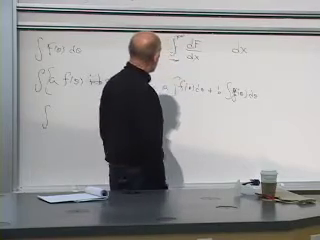
\includegraphics[width=0.88\textwidth]{lecture_06_figure_05.png}\lectureframe{01:26:31.594}\caption{Modèle ordinaire de l’intégration de Berezin : l’intégrale d’une dérivée totale se réduit aux valeurs aux bornes et s’annule lorsque la fonction tend vers zéro à l’infini. La ligne inférieure du tableau est en partie masquée ; l’équation est donc reproduite clairement dans le texte.}\end{figure}

Nous voulons que l’intégrale de Grassmann soit linéaire et possède la propriété utile selon laquelle l’intégrale d’une dérivée totale est nulle. Pour une coordonnée impaire, imposons
\begin{align}
\int d\theta\,[af(\theta)+bg(\theta)]
&=
a\int d\theta\,f(\theta)
+b\int d\theta\,g(\theta),\\
\int d\theta\,\partial_\theta f(\theta)&=0.
\end{align}
La seconde condition est l’analogue algébrique de l’invariance par translation de la mesure. Il n’y a ni bornes sur une droite des nombres impairs ni somme sur de petits intervalles.

\begin{classroomqa}\audiencequestion{S’il n’existe pas d’intégrale indéfinie de Grassmann, renonce-t-on à l’idée que l’intégration est l’opération inverse de la dérivation ? \lecturetimestamp{01:21:19}}\lecturerresponse{Oui. L’intégration de Berezin est une forme linéaire définie, et non une opération de recherche de primitive. Pour une variable de Grassmann, elle est en fait représentée par la même opération algébrique que la dérivation.}\end{classroomqa}

\begin{classroomqa}\audiencequestion{L’intégration sur tout l’espace-temps, \(d^4x\), est-elle elle aussi une intégrale définie ? \lecturetimestamp{01:21:34}}\lecturerresponse{Oui. Les conditions aux limites sont sous-entendues lorsqu’on intègre l’action sur l’espace-temps. La différence est que l’intégration ordinaire sur l’espace-temps peut se comprendre comme une limite de sommes, tandis que l’intégration de Grassmann est définie algébriquement par son action sur la base finie \(1,\theta\).}\end{classroomqa}

\subsection{Une variable}

Toute fonction d’une variable impaire peut s’écrire en plaçant son coefficient dans l’ordre fixé, à droite :
\begin{equation}
f(\theta)=a+\theta b.
\end{equation}
Comme \(\partial_\theta\theta=1\), la règle de dérivée totale implique
\begin{equation}
\int d\theta\,1=0.
\end{equation}
On choisit la normalisation restante de sorte que
\begin{equation}
\int d\theta\,\theta=1.
\end{equation}
Par conséquent,
\begin{equation}
\int d\theta\,f(\theta)=b.
\end{equation}
L’intégrale extrait le coefficient de la plus grande puissance possible. Avec la convention de dérivation à gauche utilisée ici,
\begin{equation}
\partial_\theta f=b
=\int d\theta\,f.
\end{equation}

\begin{classroomqa}\audiencequestion{Existe-t-il une fonction \(F(\theta)\) telle que \(\partial_\theta F=\theta\) ? \lecturetimestamp{01:30:05}}\lecturerresponse{Non. Une telle fonction devrait comporter un terme proportionnel à \(\theta^2\), mais \(\theta^2=0\). C’est une autre façon de voir pourquoi il n’existe pas d’analogue de la primitive indéfinie pour les variables de Grassmann.}\end{classroomqa}

\subsection{Deux variables et l’ordre de la mesure}

Pour une paire complexe \(\theta,\bar\theta\), écrivons une fonction paire générale sous la forme ordonnée
\begin{equation}
f(\theta,\bar\theta)
=a+\bar\theta\psi+\bar\psi\theta+b\,\bar\theta\theta.
\end{equation}
Il n’existe pas de terme d’ordre supérieur, car
\begin{equation}
\theta^2=\bar\theta^2=0,
\qquad
\bar\theta\theta=-\theta\bar\theta.
\end{equation}

Fixons maintenant la convention
\begin{equation}
\int d\theta\,d\bar\theta\,
\bar\theta\theta=1.
\end{equation}
Dans les intégrales itérées, l’opération \(d\bar\theta\) adjacente agit en premier. On obtient alors le tableau suivant :
\begin{align}
\int d\theta\,d\bar\theta\,1&=0,\\
\int d\theta\,d\bar\theta\,\theta&=0,\\
\int d\theta\,d\bar\theta\,\bar\theta&=0,\\
\int d\theta\,d\bar\theta\,\bar\theta\theta&=1.
\end{align}
Ainsi,
\begin{equation}
\int d\theta\,d\bar\theta\,
f(\theta,\bar\theta)=b.
\end{equation}

\begin{classroomqa}\audiencequestion{Pour un terme linéaire en \(\theta\), est-ce bien l’intégration par rapport à \(\theta\) qui rend l’intégrale double nulle ? \lecturetimestamp{01:34:59}}\lecturerresponse{Non ; l’explication donnée oralement inversait les rôles. L’intégration par rapport à \(\theta\) de \(\theta\) donne un. Le résultat ne contient alors plus de \(\bar\theta\), et l’intégrale restante de un par rapport à \(\bar\theta\) s’annule. Dans tous les cas, l’intégrale double n’est non nulle que si les deux variables sont présentes.}\end{classroomqa}

\begin{classroomqa}\audiencequestion{Si l’on intervertit \(\theta\) et \(\bar\theta\), l’intégrale change-t-elle de signe ? \lecturetimestamp{01:36:33}}\lecturerresponse{Oui. Les variables impaires et les mesures impaires anticommutent. Avec la convention ci-dessus,
\[
\int d\bar\theta\,d\theta\,\bar\theta\theta=-1.
\]
Il faut donc choisir un ordre et le respecter systématiquement. La physique est indépendante de la convention, mais les signes intermédiaires ne le sont pas.}\end{classroomqa}

Pour \(n\) variables de Grassmann indépendantes, la règle est immédiate :
\begin{equation}
\int d\theta_n\cdots d\theta_1\,
f(\theta_1,\ldots,\theta_n)
\end{equation}
extrait le coefficient du monôme ordonné de plus haut degré
\(\theta_1\cdots\theta_n\), au signe près, lequel est fixé par l’ordre choisi pour les variables et les mesures. Cette simple règle d’extraction des composantes est au cœur des actions en espace supersymétrique. Une variation supersymétrique devient une dérivée totale impaire, que l’intégrale sur l’espace supersymétrique élimine, tout comme une action ordinaire élimine une dérivée totale dans l’espace-temps lorsque les conditions aux limites le permettent.

\section{Pourquoi un calcul si élémentaire a-t-il autant de puissance}

Les règles semblent presque triviales :
\begin{equation}
\int d\theta\,1=0,
\qquad
\int d\theta\,\theta=1.
\end{equation}
Pourtant, elles nous permettent de construire des théories des champs avec interactions dans lesquelles les relations entre masses et constantes de couplage bosoniques et fermioniques sont automatiquement préservées. Le calcul en espace supersymétrique a le même objectif que le calcul tensoriel en relativité : organiser la notation de façon que la symétrie recherchée soit préservée par toutes les manipulations autorisées.

La gestion des signes en est le prix. Chaque permutation de deux objets impairs introduit un signe moins, et un calcul peut être juste sur le plan conceptuel tout en comportant une erreur due à un seul choix d’ordre. Cette difficulté n’est pas accessoire ; elle est le reflet algébrique de la statistique fermionique.

\begin{classroomqa}\audiencequestion{Les nombres de Grassmann ont-ils été inventés en même temps que la supersymétrie, ou existaient-ils déjà ? \lecturetimestamp{01:41:19}}\lecturerresponse{Ils sont bien plus anciens. Hermann Grassmann a développé l’algèbre extérieure sous-jacente au dix-neuvième siècle. Les formes différentielles utilisent déjà des éléments de base anticommutants ; la théorie quantique des champs et la supersymétrie du vingtième siècle ont donné un nouveau rôle physique à ces mêmes mathématiques.}\end{classroomqa}

Nous sommes maintenant prêts à passer à des constructions concrètes. Les superchamps regroupent des multiplets boson-fermion complets, les dérivées dans l’espace supersymétrique préservent l’algèbre, et l’intégration de Berezin extrait l’action en composantes. L’étape suivante consiste à utiliser cet outillage dans le modèle le plus simple à une dimension, puis à le transposer à la théorie des champs.

\chapter{Superspace et construction de la dynamique supersymétrique}

\lectureoverview{Nous reconstruisons la supersymétrie à partir du système le plus simple sur lequel elle peut agir : un oscillateur bosonique et un oscillateur fermionique de même énergie. Le contraste entre leurs équations du deuxième et du premier ordre conduit aux charges supersymétriques et à leur algèbre. Nous réinterprétons ensuite cette algèbre comme une géométrie sur un espace muni de la coordonnée ordinaire (t) et des coordonnées de Grassmann \(\theta,\bar\theta\). Les superchamps réunissent les bosons, les fermions et un champ auxiliaire en un seul objet ; l’intégration de Berezin extrait un lagrangien ordinaire invariant ; les dérivées covariantes permettent d’imposer des contraintes compatibles avec la symétrie ; et la contrainte chirale en fournit le premier exemple important. Le cours met délibérément en évidence les difficultés liées aux signes et à l’ordre des facteurs dans ce formalisme, puis s’achève en expliquant pourquoi la symétrie elle-même est plus fondamentale qu’un catalogue de règles de Feynman.}

\section{Retour au système à un seul mode}

Repartons des fermions et des bosons au repos. Nous supprimons toutes les coordonnées spatiales et tous les indices de quantité de mouvement. Dans un mode donné, un quantum est présent ou absent ; les opérateurs de création et d’annihilation suffisent à le décrire. Notons \(a^\dagger,a\) un mode bosonique et \(c^\dagger,c\) un mode fermionique. Ils vérifient
\begin{align}
[a,a^\dagger]&=1,
&
\{c,c^\dagger\}&=1,
&
c^2=(c^\dagger)^2&=0.
\end{align}
Si les deux quanta ont la même énergie \(m\), alors, à une constante de vide sans importance près,
\begin{equation}
H=m\left(a^\dagger a+c^\dagger c\right).
\label{eq:l7-one-mode-hamiltonian}
\end{equation}
L’opérateur nombre \(a^\dagger a\) peut prendre toute valeur entière non négative, tandis que \(c^\dagger c\) ne peut valoir que zéro ou un. Toute la cinématique de ce modèle jouet se résume à cela.

Cette simplification est stratégique. Nous voulons comprendre l’opération qui élimine un boson et crée un fermion, ou fait l’inverse, sans modifier l’énergie. Avant de construire cette opération, traduisons toutefois le même système du langage des opérateurs en langage lagrangien.

\section{L’oscillateur bosonique}

Pour le boson, introduisons une coordonnée réelle \(\phi(t)\). En l’absence de variation spatiale, un champ scalaire libre devient un oscillateur harmonique ordinaire. La première expression écrite au tableau était
\[
\frac{1}{2}\dot\phi^{,2}+\frac{1}{2}m^2\phi^2.
\]
Cette expression est l’énergie cinétique plus l’énergie potentielle, et non le lagrangien. Le cours corrige aussitôt le signe :
\begin{equation}
L_B=\frac{1}{2}\dot\phi^{,2}-\frac{1}{2}m^2\phi^2.
\label{eq:l7-boson-lagrangian}
\end{equation}

\begin{figure}[H]
\centering
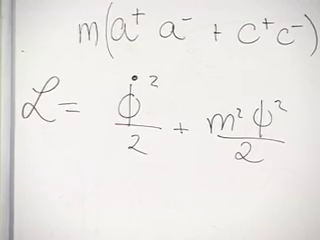
\includegraphics[width=0.62\textwidth]{lecture_07_figure_02.png}
\lectureframe{00:03:25.431}
\caption{L’hamiltonien à un mode au-dessus du lagrangien bosonique. L’image conserve le signe plus initial avant la correction formulée à l’oral vers \(T-V\).}
\end{figure}

\begin{classroomqa}
\audiencequestion{Qu’est-ce qui ne va pas dans le signe du lagrangien de l’oscillateur affiché ? \lecturetimestamp{00:04:00}}
\lecturerresponse{L’énergie est \(T+V\), mais le lagrangien est \(T-V\). Le terme de potentiel doit donc porter un signe moins. Cette correction remplace le comportement exponentiel par l’oscillation harmonique attendue.}
\end{classroomqa}

En effet, l’équation d’Euler--Lagrange donne
\begin{align}
\frac{d}{dt}\frac{\partial L_B}{\partial\dot\phi}
&=\frac{\partial L_B}{\partial\phi},\\
\ddot\phi&=-m^2\phi,
\end{align}ou
\begin{equation}
\ddot\phi+m^2\phi=0.
\label{eq:l7-boson-eom}
\end{equation}
Sa fréquence est \(m\), et non \(m^2\). La quantification de cet oscillateur produit la même échelle d’états que celle décrite par \(a^\dagger\) et \(a\) dans l’équation~\eqref{eq:l7-one-mode-hamiltonian}.

\section{Pourquoi l’action fermionique est du premier ordre}

Le lagrangien fermionique paraît plus simple parce qu’il ne contient qu’une dérivée temporelle. On en voit déjà la raison dans un essai délibérément naïf. Pour une variable ordinaire commutative,
\begin{equation}
L_{\mathrm{trial}}=\phi\dot\phi
=\frac{1}{2}\frac{d}{dt}\phi^2.
\end{equation}
C’est une dérivée totale. Son équation d’Euler--Lagrange indique seulement \(\dot\phi=\dot\phi\), de sorte que toute trajectoire différentiable est permise. Soustraire une dérivée totale à l’action modifie les données aux extrémités, mais pas l’équation du mouvement dans le volume.

Renommons maintenant la variable \(\psi\) et déclarons-la impaire de Grassmann. \(\psi\) et \(\dot\psi\) anticommutent. Avec un choix fixé de variation à gauche, la permutation des facteurs impairs introduit un signe moins ; le même essai formel donne donc
\begin{equation}
\frac{d}{dt}\frac{\partial L_{\mathrm{trial}}}{\partial\dot\psi}
=\dot\psi,
\qquad
\frac{\partial L_{\mathrm{trial}}}{\partial\psi}
=-\dot\psi.
\end{equation}
L’équation est alors
\begin{equation}
\dot\psi=-\dot\psi
\quad\Longrightarrow\quad
\dot\psi=0.
\label{eq:l7-constant-fermion}
\end{equation}
L’expression qui était une tautologie pour une coordonnée commutative acquiert un contenu dynamique pour une variable anticommutative. Ce contenu est trop contraignant pour un oscillateur, puisqu’il n’autorise qu’une constante, mais c’est précisément l’indice dont nous avons besoin.

\begin{classroomqa}
\audiencequestion{La solution consiste-t-elle simplement à dire que \(\psi\) est constante ? \lecturetimestamp{00:13:57}}
\lecturerresponse{Oui. L’équation~\eqref{eq:l7-constant-fermion} est une véritable équation différentielle du premier ordre, dont la solution est une constante arbitraire à valeurs de Grassmann. Un terme de masse transformera cette solution statique en une solution oscillante.}
\end{classroomqa}

La tentative évidente, \(m\psi^2\), échoue parce que \(\psi^2=0\). Il nous faut deux variables réelles impaires \(\psi_1,\psi_2\), ou, de manière équivalente, une variable complexe et sa conjuguée. Le cours développe au tableau la formulation à deux variables réelles, en vérifiant à plusieurs reprises les signes et les facteurs de deux. Une formulation complexe normalisée selon la convention usuelle est
\begin{equation}
L_F=\frac{i}{2}
\left(\bar\psi\dot\psi-\dot{\bar\psi}\psi\right)
-m\bar\psi\psi.
\label{eq:l7-fermion-lagrangian}
\end{equation}
À une dérivée totale près, cela donne \(i\bar\psi\dot\psi-m\bar\psi\psi\). La variation par rapport à \(\bar\psi\) donne
\begin{equation}
i\dot\psi=m\psi,
\qquad
\psi(t)=\psi(0)e^{-imt}.
\label{eq:l7-fermion-eom}
\end{equation}
L’équation conjuguée a une phase opposée. Le mode fermionique oscille donc avec l’énergie \(m\), comme le mode bosonique, bien que son équation soit du premier ordre et non du deuxième.

\editorialnote{L’équation~\eqref{eq:l7-fermion-lagrangian} fixe un ordre et une normalisation standard pour le calcul exploratoire à deux variables réelles. Dans le cours, le facteur \(i\) est inséré, un facteur deux est ajusté et le signe d’une composante réelle reste indéterminé. Ces changements ne modifient pas la conclusion centrale : la cinétique des fermions est du premier ordre, la masse intervient linéairement et un fermion complexe fournit un bilinéaire non nul.}

C’est l’ombre, en dimension zéro, d’un contraste relativiste bien connu. L’équation de Klein--Gordon est du deuxième ordre en temps, tandis que l’équation de Dirac est du premier ordre. Lorsque l’on supprime les coordonnées spatiales, le boson devient un oscillateur harmonique et le fermion, un oscillateur complexe de Grassmann.

\begin{classroomqa}
\audiencequestion{L’ordre dans lequel on écrit \(\psi\), \(\dot\psi\) et leurs conjugués a-t-il de l’importance ? \lecturetimestamp{00:18:58}}
\lecturerresponse{Les formules intermédiaires dépendent bien de l’ordre, car les facteurs impairs anticommutent. La théorie physique ne dépend pas d’un choix arbitraire de notation, à condition d’appliquer partout une même convention pour les variations à gauche ou à droite, la conjugaison et l’intégration. Inverser l’ordre de deux facteurs impairs change un signe ; il faut alors modifier de manière cohérente tous les autres signes concernés.}
\end{classroomqa}

En combinant les équations~\eqref{eq:l7-boson-lagrangian} et \eqref{eq:l7-fermion-lagrangian}, on obtient une description lagrangienne de la même paire appariée que celle représentée par l’équation~\eqref{eq:l7-one-mode-hamiltonian}. Nous pouvons maintenant identifier la symétrie qui les relie.

\section{Les charges supersymétriques et leur algèbre}

Un opérateur qui élimine un fermion et crée un boson est
\begin{equation}
Q^\dagger=\sqrt{2m}\,a^\dagger c,
\end{equation}
tandis que son conjugué élimine un boson et crée un fermion,
\begin{equation}
Q=\sqrt{2m}\,a c^\dagger.
\end{equation}
La normalisation est choisie de façon à obtenir la forme standard de l’algèbre. En utilisant \(cc^\dagger=1-c^\dagger c\), \(aa^\dagger=a^\dagger a+1\) et le fait que les opérateurs bosoniques commutent avec les opérateurs fermioniques,
\begin{align}
\{Q,Q^\dagger\}
&=2m\left(ac^\dagger a^\dagger c+a^\dagger c a c^\dagger\right)\notag\\
&=2m\left[(a^\dagger a+1)c^\dagger c
+a^\dagger a(1-c^\dagger c)\right]\notag\\
&=2m\left(a^\dagger a+c^\dagger c\right)=2H.
\label{eq:l7-superalgebra}
\end{align}
On peut déplacer les opérateurs bosoniques au travers des opérateurs fermioniques. La même nilpotence qui limite l’occupation fermionique donne
\begin{equation}
Q^2=(Q^\dagger)^2=0.
\end{equation}
Enfin,
\begin{equation}
[H,Q]=[H,Q^\dagger]=0.
\label{eq:l7-conserved-supercharges}
\end{equation}
Chaque charge supersymétrique modifie le nombre de bosons et le nombre de fermions en sens opposés ; les deux variations d’énergie s’annulent donc lorsque les fréquences sont égales.

\begin{classroomqa}
\audiencequestion{Que vaut \([H,Q]\) ? La réponse est-elle proportionnelle à \(Q\) ? \lecturetimestamp{00:25:10}}
\lecturerresponse{Non. La réponse est zéro. Un opérateur de création ou d’annihilation isolé acquiert son énergie lorsqu’on le commute avec \(H\), mais les contributions bosonique et fermionique dans \(Q\) s’annulent. Cette annulation est précisément la condition d’égalité des énergies.}
\end{classroomqa}

\begin{classroomqa}
\audiencequestion{Cette relation de commutation n’avait-elle pas déjà été écrite au tableau ? \lecturetimestamp{00:25:45}}
\lecturerresponse{Si. La redécouvrir est utile, car cela nous oblige à interpréter la relation plutôt qu’à la recopier : commuter avec l’hamiltonien signifie que la transformation est une symétrie et que son générateur est conservé.}
\end{classroomqa}

Le qualificatif \emph{charge} renvoie à cette loi de conservation. Il ne faut toutefois pas considérer \(Q\) comme un nombre ordinaire, mesurable simultanément, associé à un état. Cette quantité est impaire de Grassmann, nilpotente et transforme un état bosonique en état fermionique. L’énoncé utile est qu’il s’agit d’un générateur conservé qui agit au sein de supermultiplets dégénérés.
\editorialnote{Cette formulation précise l’analogie faite en cours avec la classification des états par leur énergie ou leur charge électrique. Les charges supersymétriques impaires, prises individuellement et non hermitiennes, ne sont pas des observables ordinaires auxquelles correspondent des nombres quantiques. C’est leur action conservée et la représentation de l’ensemble de la superalgèbre qui fournissent la classification correcte.}

\section{Les générateurs comme dérivées}

L’algèbre est compacte, mais elle ne nous indique pas à elle seule comment construire des théories avec interactions. L’étape suivante est géométrique. Les générateurs des symétries usuelles agissent déjà comme des opérateurs différentiels. Dans la convention du cours,
\begin{equation}
H=i\frac{\partial}{\partial t},
\qquad
P=-i\frac{\partial}{\partial x}.
\end{equation}

\begin{figure}[H]
\centering
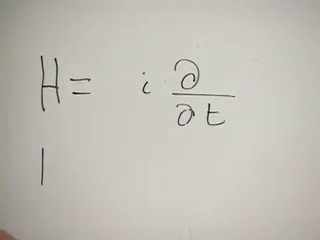
\includegraphics[width=0.50\textwidth]{lecture_07_figure_03.png}
\lectureframe{00:28:12.720}
\caption{L’hamiltonien représenté comme générateur des translations temporelles.}
\end{figure}

Le moment cinétique est lui aussi un produit d’une coordonnée et d’une dérivée. Si les charges supersymétriques sont des générateurs impairs, on peut naturellement se demander si elles peuvent être représentées par des dérivées par rapport à des coordonnées impaires. Nous étendons donc l’axe temporel en le remplaçant par le superspace
\begin{equation}
(t,\theta,\bar\theta),
\qquad
\theta^2=\bar\theta^2=0,
\qquad
\theta\bar\theta=-\bar\theta\theta.
\end{equation}
Les champs sur cet espace dépendent du temps ordinaire et d’une paire conjuguée de coordonnées de Grassmann.

Le cours montre délibérément à quel point les signes sont délicats. Le signe provenant de la conjugaison complexe, celui provenant du déplacement d’un paramètre impair et celui qui découle du choix de dérivées à gauche plutôt qu’à droite correspondent à des opérations différentes. Au lieu de conserver des étapes au tableau mutuellement incompatibles, fixons une convention : toutes les dérivées impaires sont des dérivées à gauche, et
\begin{equation}
q=\partial_\theta+i\bar\theta\partial_t,
\qquad
\bar q=\partial_{\bar\theta}+i\theta\partial_t.
\label{eq:l7-differential-supercharges}
\end{equation}
Alors
\begin{equation}
q^2=\bar q^{,2}=0,
\qquad
\{q,\bar q\}=2i\partial_t=2H.
\label{eq:l7-differential-algebra}
\end{equation}
Le facteur deux provient de deux termes croisés : \(\{\partial_\theta,\theta\}=1\) et \(\{\partial_{\bar\theta},\bar\theta\}=1\). Si les générateurs ne contenaient que \(\partial_\theta\) et \(\partial_{\bar\theta}\), leur anticommutateur s’annulerait et ne pourrait pas reproduire l’hamiltonien.

\begin{classroomqa}
\audiencequestion{Les deux termes de dérivée temporelle dans \(q\) et \(\bar q\) doivent-ils avoir le même signe ? \lecturetimestamp{00:31:01}}
\lecturerresponse{Il faut choisir leurs signes de manière cohérente afin que l’anticommutateur mixte soit \(2H\). On peut adopter une convention avec un signe plus global, ou l’alternative conjuguée de manière cohérente. C’est le calcul, et non l’intuition visuelle associée au symbole \(i\), qui fixe les signes relatifs.}
\end{classroomqa}

Dans la salle, les signes sont vérifiés à plusieurs reprises, et leur difficulté devient un sujet de plaisanterie : ils semblent changer pendant le trajet pour aller travailler. La plaisanterie est bien trouvée. Faire passer un paramètre de Grassmann au travers d’une coordonnée peut changer un signe, même si aucune convention physique n’a changé. L’équation~\eqref{eq:l7-differential-supercharges} est la référence fixe pour tout ce qui suit.

\subsection{La supersymétrie comme déplacement de coordonnées}

Soient \(\xi,\bar\xi\) des paramètres impairs infinitésimaux. L’action sur un superchamp de
\begin{equation}
\delta_\xi=\xi q+\bar\xi\bar q
\end{equation}
équivaut, dans la convention ci-dessus, au changement infinitésimal de coordonnées
\begin{align}
\theta&\longrightarrow\theta+\xi,\\
\bar\theta&\longrightarrow\bar\theta+\bar\xi,\\
t&\longrightarrow t+i\left(\xi\bar\theta+\bar\xi\theta\right).
\label{eq:l7-coordinate-shift}
\end{align}
La variation d’un superchamp scalaire est donc
\begin{equation}
\delta_\xi\Phi
=\left(\xi\partial_\theta+\bar\xi\partial_{\bar\theta}
+i\xi\bar\theta\partial_t+i\bar\xi\theta\partial_t\right)\Phi
=\left(\xi q+\bar\xi\bar q\right)\Phi.
\end{equation}
Voilà le contenu géométrique de la supersymétrie. Il s’agit d’une translation dans les directions impaires, liée à une translation du temps ordinaire. La composition de deux déplacements impairs donne une translation temporelle, conformément à l’équation~\eqref{eq:l7-differential-algebra}.

\begin{classroomqa}
\audiencequestion{Le signe moins contesté pourrait-il représenter un déplacement vers le passé ? \lecturetimestamp{00:58:13}}
\lecturerresponse{Une convention différente pour les signes peut inverser le déplacement temporel infinitésimal affiché, mais elle n’introduit aucun processus physique distinct de retour dans le temps. L’essentiel est que la transformation des coordonnées et les générateurs différentiels obéissent à la même algèbre.}
\end{classroomqa}

\begin{classroomqa}
\audiencequestion{Ce temps étendu a-t-il une réalisation physique, ou s’agit-il seulement d’un artifice de calcul ? \lecturetimestamp{00:58:23}}
\lecturerresponse{C’est un artifice de calcul en un sens utile : il intègre l’algèbre à une géométrie. Mais cet artifice devient physiquement précieux lorsqu’on introduit des interactions. Le superspace fournit un calcul systématique pour construire des lagrangiens qui préservent à chaque étape la symétrie boson--fermion, tout comme le calcul tensoriel aide à construire des scalaires de Lorentz.}
\end{classroomqa}

\section{Superchamps et composante auxiliaire}

Comme il n’y a que deux coordonnées impaires, le développement d’un superchamp pair s’arrête :
\begin{equation}
\Phi(t,\theta,\bar\theta)
=\phi(t)+\bar\theta\psi(t)+\bar\psi(t)\theta
+D(t)\bar\theta\theta.
\label{eq:l7-superfield}
\end{equation}
Les coefficients des monômes pairs, \(\phi\) et \(D\), sont bosoniques ; ceux des monômes impairs, \(\psi\) et \(\bar\psi\), sont fermioniques. Aucun terme \(\theta^2\), \(\bar\theta^2\) ou d’ordre supérieur ne subsiste. Nous ne développons pas la dépendance temporelle, car un développement de Taylor ordinaire en \(t\) ne s’arrêterait pas et serait sans utilité ici.

\begin{classroomqa}
\audiencequestion{Que représente la composante \(D(t)\) dans le terme de plus haut degré ? \lecturetimestamp{00:41:46}}
\lecturerresponse{À ce stade, il s’agit simplement du dernier coefficient bosonique dans le développement fini. Dans l’action en composantes, elle n’a généralement pas de terme cinétique et est éliminée par une équation du mouvement algébrique ; on l’appelle donc champ auxiliaire. Le cours propose sur le ton de la plaisanterie ``D pour dummy (auxiliaire),'' ce qui décrit son rôle non dynamique sans pour autant constituer l’origine historique de cette appellation.}
\end{classroomqa}

Le superchamp est un objet unique, tandis que \(\phi,\psi,\bar\psi,D\) en sont les composantes. Une transformation supersymétrique les mélange. Un boson et un fermion sont donc reliés selon une structure très semblable à celle qui relie, par une rotation, les composantes selon \(x\) et \(y\) d’un vecteur, même si les directions de Grassmann ne peuvent pas être représentées comme des axes ordinaires.

\section{La superaction et la composante de plus haut degré}

Pour obtenir les équations du mouvement, il nous faut une action. En théorie des champs ordinaire, on forme un lagrangien scalaire et on l’intègre sur l’espace-temps. Ici, l’expression analogue est
\begin{equation}
S=\int dt\,d\theta\,d\bar\theta\;\Lambda
\bigl(\Phi,\text{ superspace derivatives of }\Phi\bigr),
\label{eq:l7-superaction}
\end{equation}
où \(\Lambda\) est un superchamp pair. L’intégration de Berezin est algébrique. Choisissons
\begin{equation}
\int d\theta\,d\bar\theta\;\bar\theta\theta=1.
\end{equation}
Par conséquent, si
\begin{equation}
\Lambda=A+\bar\theta B+\bar B\theta+C\bar\theta\theta,
\end{equation}
alors
\begin{equation}
\int d\theta\,d\bar\theta\;\Lambda=C.
\label{eq:l7-top-component}
\end{equation}
L’intégration sur les variables impaires extrait la composante de plus haut degré et laisse un lagrangien ordinaire à intégrer sur le temps.

Pourquoi le résultat est-il invariant ? Une variation supersymétrique translate les variables d’intégration. La variation de la composante de plus haut degré est une dérivée totale ordinaire par rapport au temps, tandis que les dérivées totales impaires s’annulent dans l’intégration de Berezin. Sous des conditions convenables aux extrémités, l’action reste inchangée. C’est l’analogue, dans le superspace, de la construction d’un scalaire de Lorentz avant son intégration sur l’espace-temps.

\section{Multiplication de superchamps}

Le moyen le plus simple de construire un nouveau superchamp à partir d’un autre est de le multiplier par lui-même. En partant de l’équation~\eqref{eq:l7-superfield}, tous les termes contenant \(\theta^2\) ou \(\bar\theta^2\) s’annulent. En conservant l’ordre \(\bar\theta\theta\) et en plaçant à gauche les champs composantes barrés, on obtient
\begin{align}
\Phi^2
={}&\phi^2
+2\phi\bar\theta\psi
+2\phi\bar\psi\theta\notag\\
&+\left(2\phi D-2\bar\psi\psi\right)\bar\theta\theta.
\label{eq:l7-superfield-square}
\end{align}

\begin{figure}[H]
\centering
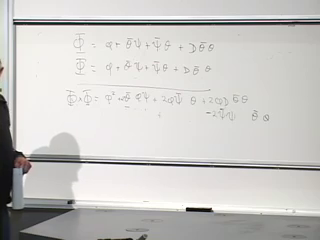
\includegraphics[width=0.82\textwidth]{lecture_07_figure_05.png}
\lectureframe{01:07:57.844}
\caption{Le produit de superchamps, développé composante par composante, et l’ensemble de ses termes en \(\bar\theta\theta\).}
\end{figure}

Les deux termes \(\phi D\) et \(D\phi\) s’additionnent parce que les deux champs sont pairs. Les deux termes croisés fermioniques s’additionnent également après permutation de leurs facteurs, mais leur signe commun est négatif :
\begin{equation}
(\bar\theta\psi)(\bar\psi\theta)
+(\bar\psi\theta)(\bar\theta\psi)
=-2\bar\psi\psi\,\bar\theta\theta.
\end{equation}
L’intégration du carré sur les coordonnées impaires donne
\begin{equation}
\int d\theta\,d\bar\theta\;\Phi^2
=2\phi D-2\bar\psi\psi.
\end{equation}
Ce terme est supersymétrique par construction, mais ce n’est pas encore un lagrangien cinétique. Il ne contient aucune dérivée temporelle.

Le cours propose ensuite \(\Phi^3\), \(\Phi^4\) et \(\Phi^n\) comme exercices. Il existe une règle compacte. Pour toute fonction ordinaire \(W\),
\begin{equation}
\left.W(\Phi)\right|_{\bar\theta\theta}
=W'(\phi)D-W''(\phi)\bar\psi\psi.
\label{eq:l7-function-top-component}
\end{equation}
Pour \(W(\phi)=\phi^2\), on retrouve l’équation~\eqref{eq:l7-superfield-square} ; pour \(W(\phi)=\phi^n\), on obtient
\begin{equation}
\left.\Phi^n\right|_{\bar\theta\theta}
=n\phi^{n-1}D-n(n-1)\phi^{n-2}\bar\psi\psi.
\end{equation}
\editorialnote{Le cours donne comme exercice la puissance \(n\) et indique les types de termes attendus. L’équation~\eqref{eq:l7-function-top-component} fournit la règle complète selon la convention d’ordre fixée.}

À ce stade, l’enseignant demande à la salle si elle est épuisée. Le public répond que non ; il répond, lui, qu’il l’est. Cet échange ne sert pas seulement de détente comique. Les puissances de superchamps sont simples, car le développement s’arrête, mais les dérivées et les contraintes sont là où le suivi des signes devient réellement exigeant.

\section{Quelles dérivées respectent la supersymétrie ?}

Il faut corriger un point avant de suivre l’argument suivant au tableau. La dérivée temporelle ordinaire ne pose pas de problème :
\begin{equation}
[\partial_t,q]=[\partial_t,\bar q]=0.
\end{equation}
Par conséquent, \(\partial_t\Phi\) se transforme comme un superchamp dès lors que \(\Phi\) le fait. Les objets subtils sont les dérivées impaires brutes \(\partial_\theta\Phi\) et \(\partial_{\bar\theta}\Phi\), car elles n’anticommutent pas avec les deux charges supersymétriques. Il nous faut des dérivées impaires modifiées pour les contraintes et pour construire des composantes manifestement supersymétriques.
\editorialnote{L’affirmation orale selon laquelle une dérivation temporelle ne produit pas un autre superchamp est incorrecte dans la convention utilisée ici. Puisque \(\partial_t\) commute avec les deux charges supersymétriques, elle est covariante. La construction ultérieure de dérivées impaires modifiées reste nécessaire et constitue le véritable point mathématique du cours.}

\subsection{L’analogie du champ ``magique''}

Le cours motive ce critère par l’exemple des rotations ordinaires. Soit \(f(x,y)\) une fonction vérifiant
\begin{equation}
\partial_y f=0.
\label{eq:l7-magic-constraint}
\end{equation}
Appelons une telle fonction un « champ ``magique'' ». Elle dépend de \(x\), mais pas de \(y\). La classe des champs magiques est-elle préservée par les rotations ? Pour
\begin{equation}
L_z=-i\left(x\partial_y-y\partial_x\right),
\end{equation}
on trouve
\begin{equation}
[\partial_y,L_z]=i\partial_x\neq0.
\end{equation}
Par conséquent, \(L_z f\) acquiert en général une dépendance en \(y\), même lorsque \(f\) vérifie initialement l’équation~\eqref{eq:l7-magic-constraint}. La contrainte n’est pas invariante par rotation.

La leçon générale est simple. Si un champ vérifie \(C\Phi=0\) et si une symétrie est engendrée par \(G\), le champ transformé reste contraint lorsque le commutateur gradué de \(C\) avec \(G\) s’annule. Pour deux opérateurs impairs, le commutateur gradué est un anticommutateur.

\begin{classroomqa}
\audiencequestion{Quand une contrainte imposée à un champ est-elle compatible avec une symétrie ? \lecturetimestamp{01:17:56}}
\lecturerresponse{Lorsque l’opérateur de contrainte commute au sens gradué avec les générateurs de la symétrie. On peut alors faire passer \(C(G\Phi)\) au travers de \(G\) et retrouver \(G(C\Phi)=0\). L’exemple des rotations échoue parce que \(\partial_y\) ne commute pas avec le générateur de rotation.}
\end{classroomqa}

\subsection{Dérivées impaires covariantes}

Les charges supersymétriques étant fixées par l’équation~\eqref{eq:l7-differential-supercharges}, définissons
\begin{equation}
\mathcal D=\partial_\theta-i\bar\theta\partial_t,
\qquad
\bar{\mathcal D}=\partial_{\bar\theta}-i\theta\partial_t.
\label{eq:l7-covariant-derivatives}
\end{equation}
Seul le signe du terme de dérivée temporelle change. Un calcul direct donne
\begin{align}
\{\mathcal D,q\}
&=\{\mathcal D,\bar q\}
=\{\bar{\mathcal D},q\}
=\{\bar{\mathcal D},\bar q\}=0,\\
\{\mathcal D,\bar{\mathcal D}\}&=-2i\partial_t.
\label{eq:l7-covariant-algebra}
\end{align}
Les deux termes croisés potentiellement non nuls s’annulent. C’est l’analogue impair d’une dérivée covariante : elle dérive tout en préservant la loi de transformation.

Le cours utilise \(D\) à la fois pour la composante auxiliaire et pour cette dérivée. Nous réservons \(D(t)\) à la composante et employons le D calligraphié \(\mathcal D\) pour l’opérateur.

\section{La contrainte chirale}

Nous pouvons maintenant imposer une contrainte non triviale qui est préservée par la supersymétrie :
\begin{equation}
\bar{\mathcal D}\Phi=0.
\label{eq:l7-chiral-constraint}
\end{equation}
Un tel champ est dit chiral. S’il est chiral avant une transformation supersymétrique, alors
\begin{equation}
\bar{\mathcal D}(q\Phi)
=-q(\bar{\mathcal D}\Phi)=0,
\qquad
\bar{\mathcal D}(\bar q\Phi)
=-\bar q(\bar{\mathcal D}\Phi)=0.
\end{equation}
Le superchamp transformé tout entier reste donc dans la classe des champs contraints. Contrairement à la condition du champ magique, la chiralité est compatible avec la symétrie.

Pour résoudre la contrainte, définissons une coordonnée temporelle décalée
\begin{equation}
\tau=t+i\bar\theta\theta.
\label{eq:l7-chiral-time}
\end{equation}
Comme nous utilisons des dérivées à gauche,
\begin{equation}
\partial_{\bar\theta}\tau=i\theta,
\end{equation}
et par conséquent
\begin{equation}
\bar{\mathcal D}F(\tau,\theta)
=\left(\partial_{\bar\theta}-i\theta\partial_t\right)F(\tau,\theta)
=i\theta\partial_\tau F-i\theta\partial_\tau F=0.
\end{equation}
Le superchamp chiral local le plus général dépend donc de \(\bar\theta\) uniquement par l’intermédiaire de \(\tau\) :
\begin{equation}
\Phi_{\mathrm{ch}}(\tau,\theta)
=\phi(\tau)+\bar\psi(\tau)\theta.
\label{eq:l7-chiral-field-tau}
\end{equation}

\begin{classroomqa}
\audiencequestion{La dépendance en \(\tau\) et \(\theta\) est-elle la seule forme satisfaisant à la contrainte chirale ? \lecturetimestamp{01:32:35}}
\lecturerresponse{Oui, localement. L’équation différentielle \(\bar{\mathcal D}\Phi=0\) signifie précisément que la dépendance indépendante en \(\bar\theta\) peut être absorbée dans la coordonnée décalée \(\tau=t+i\bar\theta\theta\). Le développement fini restant est une fonction de \(\tau\), plus un terme proportionnel à \(\theta\).}
\end{classroomqa}

En développant de nouveau selon la coordonnée temporelle d’origine,
\begin{align}
\phi(\tau)
&=\phi(t)+i\bar\theta\theta\dot\phi(t),\\
\bar\psi(\tau)\theta
&=\bar\psi(t)\theta,
\end{align}
car la correction de la deuxième ligne contient \(\theta^2\). On a donc
\begin{equation}
\Phi_{\mathrm{ch}}(t,\theta,\bar\theta)
=\phi(t)+\bar\psi(t)\theta
+i\bar\theta\theta\dot\phi(t).
\label{eq:l7-chiral-field-components}
\end{equation}

\begin{classroomqa}
\audiencequestion{Le développement de Taylor de \(\phi(t+i\bar\theta\theta)\) doit-il comporter un terme du deuxième ordre ? \lecturetimestamp{01:33:51}}
\lecturerresponse{Non. La première correction est \(i\bar\theta\theta\dot\phi\), et toutes les corrections d’ordre supérieur contiennent \((\bar\theta\theta)^2=0\). Le public le remarque immédiatement : la nilpotence a déjà fourni les deux premiers termes et interrompu le développement.}
\end{classroomqa}

Voilà la simplicité de la chiralité. Le superchamp non contraint de l’équation~\eqref{eq:l7-superfield} possède deux emplacements de composantes bosoniques et deux fermioniques. Dans cet exemple minimal à une dimension, la condition chirale supprime l’emplacement auxiliaire indépendant et relie la composante de plus haut degré à \(\dot\phi\).

\section{Le calcul qu’il vaut mieux interrompre}

L’étape suivante naturelle consiste à combiner le champ chiral avec son conjugué, puis à intégrer sur le superspace. Le développement conjugué est commencé, et une personne dans le public demande si l’ordre \(\theta\bar\theta\) doit être inversé par conjugaison. À ce stade, les signes ne semblent plus fiables. Plutôt que de bluffer, le calcul est interrompu.

\begin{classroomqa}
\audiencequestion{Peut-on donner le résultat essentiel même si le produit avec le champ conjugué est différé ? \lecturetimestamp{01:37:30}}
\lecturerresponse{Oui. En traitant de façon cohérente les signes et les conjugaisons, une expression dans le superspace construite à partir d’un champ chiral et de son conjugué produit les termes cinétiques bosonique et fermionique ordinaires attendus. Pour ce cours, le résultat important est le principe de construction, et non une ligne finale peu fiable recopiée à l’issue d’un calcul mené avec fatigue.}
\end{classroomqa}

Il faut que l’interruption reste visible. Le formalisme ne pardonne pas : une seule permutation mal placée de facteurs impairs change un signe, et la même convention doit être maintenue lors de la conjugaison, de la dérivation, de la multiplication et de l’intégration. Si l’on perd le fil de cette cohérence, il faut le rétablir avant de poursuivre. Dans une convention standard, l’action cinétique usuelle se construit à partir d’un produit avec le champ conjugué ; sa réduction détaillée en composantes relève toutefois du prochain calcul effectué proprement, et non de la reconstitution d’une ligne inachevée au tableau.

\section{Pourquoi la symétrie est le point essentiel}

Un lagrangien supersymétrique ne se contente pas de placer côte à côte un boson et un fermion. Il contraint leurs masses et leurs interactions de façon qu’ils forment une représentation de la superalgèbre. Dans un vide exactement supersymétrique, les membres d’un supermultiplet ont des masses égales. Leurs contributions en boucles sont corrélées, et les effets ultraviolets bosoniques et fermioniques s’annulent précisément dans les combinaisons imposées par la symétrie.

C’est pourquoi le formalisme de construction est important. On pourrait énumérer les sommets de Feynman et vérifier les annulations diagramme par diagramme, mais elles paraîtraient alors fortuites. La supersymétrie les explique comme la symétrie de Lorentz explique pourquoi les amplitudes de diffusion se transforment de manière cohérente dans tous les référentiels inertiels.

\editorialnote{La supersymétrie exacte n’implique pas que chaque correction individuelle d’auto-énergie s’annule. Elle relie les renormalisations et élimine certaines sensibilités ultraviolettes ; les énoncés de non-renormalisation dépendent de la quantité considérée, de la dimension et de la quantité de supersymétrie. L’affirmation générale du cours sur les annulations est conservée sous cette forme nuancée.}

\begin{classroomqa}
\audiencequestion{Comment s’écrit « ``chiral'' » ? \lecturetimestamp{01:39:48}}
\lecturerresponse{C-H-I-R-A-L. Ce mot désigne la contrainte \(\bar{\mathcal D}\Phi=0\) ; il ne renvoie pas à l’orientation géométrique habituelle d’un objet dans l’espace tridimensionnel, même si cette terminologie vient de la structure gauche et droite des spineurs relativistes.}
\end{classroomqa}

\begin{classroomqa}
\audiencequestion{Peut-on contourner le lagrangien et passer directement aux règles de Feynman supersymétriques ? \lecturetimestamp{01:40:00}}
\lecturerresponse{On peut bien sûr énoncer les règles, mais les relations entre les couplages et les annulations qu’elles produisent semblent alors être des coïncidences inexpliquées. Le contenu plus profond est celui d’une symétrie généralisée de l’espace-temps. Le lagrangien, ou une formulation invariante équivalente, rend cette raison manifeste et engendre systématiquement les règles.}
\end{classroomqa}

Supposons que, par hasard, les amplitudes soient invariantes de Lorentz à tous les ordres de la théorie des perturbations, alors même qu’aucune transformation de Lorentz n’ait été mentionnée. Après suffisamment de calculs, nous exigerions une explication. Celle-ci serait la symétrie de l’espace-temps qui organise simultanément tous les ordres. Le rôle de l’espace supersymétrique est analogue : les déplacements dans \(\theta,\bar\theta\) mélangent les composantes bosoniques et fermioniques, et leur algèbre se referme sur les translations de l’espace-temps.

\begin{classroomqa}
\audiencequestion{Faut-il aussi développer les coordonnées spatiales ordinaires en série finie, comme les coordonnées de Grassmann ? \lecturetimestamp{01:44:55}}
\lecturerresponse{Non. Une série en une coordonnée ordinaire ne s’arrête pas et ne constitue généralement pas la décomposition la plus naturelle. Une transformée de Fourier est plus utile, car elle décompose un champ en ondes et en impulsions. Le développement en \(\theta\) est particulier précisément parce que la nilpotence le rend fini.}
\end{classroomqa}

\begin{classroomqa}
\audiencequestion{Si une nouvelle particule était découverte au LHC, comment pourrions-nous savoir qu’il s’agit d’un superpartenaire plutôt que d’une simple particule inconnue ? \lecturetimestamp{01:45:42}}
\lecturerresponse{La supersymétrie prédit des nombres quantiques et des interactions corrélés, et pas seulement un état supplémentaire. Les spins diffèrent d’une demi-unité, les charges de jauge sont liées, et de nombreux couplages cubiques et quartiques dépendent d’un nombre de paramètres indépendants inférieur à celui d’une théorie générique. Les sections efficaces, les fractions de branchement et le reste du spectre devraient respecter ces relations.}
\end{classroomqa}

Une résonance inconnue ne suffirait pas, à elle seule, à prouver la supersymétrie. C’est un réseau de relations entre les couplages et les spectres qui le ferait. Voilà le pendant expérimental de la construction en espace supersymétrique : des interactions entre composantes apparemment indépendantes découlent d’un seul objet invariant.

\begin{classroomqa}
\audiencequestion{Les particules observées et leurs superpartenaires hypothétiques n’ont pas la même masse. Qu’est-ce que cela change à la théorie ? \lecturetimestamp{01:47:01}}
\lecturerresponse{Cela la change énormément. La supersymétrie doit être brisée, généralement par une brisure spontanée communiquée au secteur observé. Cette brisure sépare les masses des multiplets tout en préservant suffisamment de la structure pour contrôler les interactions et, si l’échelle est assez basse, les corrections ultraviolettes. Élaborer ce mécanisme constitue une théorie importante à part entière, en particulier lorsque la gravité est prise en compte.}
\end{classroomqa}

\section{Principe simple, calcul difficile}

Le bilan final est d’une franchise inhabituelle. L’idée de départ paraît simple : les bosons et les fermions sont reliés par une symétrie. Pourtant, sa mise en œuvre devient vite une discipline faite d’indices, de conjugaisons, d’ordres des variables de Grassmann et de signes. Même après avoir construit la symétrie, la physique des particules réaliste exige de la briser ; son couplage à la gravité mène à la supergravité et ajoute un niveau supplémentaire de structure.

Cette difficulté ne prouve pas que l’idée soit vide. La nature n’a aucune obligation de rendre facile le calcul fondé sur un principe simple. Les spécialistes apprennent la matière en reprenant les détails jusqu’à ce que les règles de signes deviennent instinctives. La frustration vient de l’écart entre la brièveté de l’algèbre
\begin{equation}
\{Q,Q^\dagger\}=2H
\end{equation}
et la quantité d’outils nécessaires pour la mettre en œuvre dans une théorie avec interactions.

\begin{classroomqa}
\audiencequestion{Un niveau supplémentaire d’abstraction finit-il par simplifier le formalisme, ou les complications ne cessent-elles de s’accumuler ? \lecturetimestamp{01:49:33}}
\lecturerresponse{Aucune simplification générale n’a éliminé le travail de détail. Les règles fondamentales peuvent être brèves, mais leur application fiable exige de maîtriser les conventions à force de les reprendre. C’est pourquoi un traitement complet occupe normalement tout un cours technique plutôt qu’une fraction d’un cours général de physique des particules.}
\end{classroomqa}

\begin{classroomqa}
\audiencequestion{Les transformations nous disent-elles ce que sont réellement les fermions et les bosons, ou pourquoi leur comportement ordinaire diffère ? \lecturetimestamp{01:51:42}}
\lecturerresponse{Elles nous disent que les deux sont des composantes d’un même superchamp et des images l’une de l’autre sous l’action des supercharges. L’action de \(Q\) transforme une composante bosonique en une composante fermionique, tandis que la transformation suivante produit des dérivées et des composantes auxiliaires. Cela ressemble à une rotation qui mélange les composantes d’un vecteur, mais on ne peut pas en donner une image aussi littérale : le langage approprié est celui de la géométrie de Grassmann elle-même.}
\end{classroomqa}

Cette réponse nous ramène à l’idée centrale. Une transformation supersymétrique est un petit déplacement dans l’espace supersymétrique. Elle mélange \(\phi,\psi,\bar\psi,D\) comme une rotation ordinaire mélange des composantes, tout en se refermant sur une translation dans le temps. L’image est abstraite, mais elle n’est pas arbitraire : chaque terme du superchamp, chaque signe des dérivées covariantes et chaque relation entre les interactions des composantes sont là pour réaliser l’algèbre.

\section{Ce que nous avons construit}

Nous sommes partis de l’hamiltonien d’oscillateur apparié et avons retrouvé ses deux descriptions lagrangiennes distinctes. Le boson obéit à une équation d’oscillateur du second ordre ; le fermion exige une action de Grassmann du premier ordre et une paire complexe de composantes impaires. Les supercharges échangent les deux modes, chacune est de carré nul, leur anticommution donne l’hamiltonien, et elles commutent avec celui-ci.

La représentation de ces charges par des opérateurs différentiels nous a conduits à l’espace supersymétrique. Un développement fini du superchamp réunit les composantes bosoniques, fermioniques et auxiliaires ; l’intégration de Berezin sélectionne la composante supérieure d’un superlagrangien ; et la multiplication produit des termes d’interaction possibles invariants. Exiger une dérivation impaire compatible avec la symétrie nous a ensuite conduits à \(\mathcal D,\bar{\mathcal D}\), à la contrainte chirale et à la coordonnée décalée \(\tau=t+i\bar\theta\theta\).

Le calcul inachevé du produit par son conjugué fait partie de la leçon ; ce n’est pas un défaut à dissimuler. La supersymétrie part d’une exigence physique simple, mais son calcul dépend de chaque choix d’ordre. Une fois ces choix maîtrisés, le résultat est puissant : la symétrie organise les masses et les couplages, les corrections quantiques satisfont des relations qui ne sont pas fortuites, et les bosons et les fermions deviennent les composantes d’un même objet géométrique.

\chapter{Supersymétrie en quatre dimensions et modèle de Wess--Zumino}

\lectureoverview{L’algèbre de supersymétrie unidimensionnelle du cours précédent ne faisait intervenir que le Hamiltonien. L’invariance de Lorentz impose maintenant de réunir l’énergie et l’impulsion spatiale, et les supercharges doivent devenir des spineurs à deux composantes. Pour obtenir cette algèbre, reprenons d’abord une fermion de Weyl sans masse et son Hamiltonien \(H=\boldsymbol{\sigma}\cdot\mathbf p\). Nous représenterons ensuite les supercharges par des opérateurs différentiels sur l’espace-temps supersymétrique à quatre dimensions, isolerons les superchamps chiraux au moyen de la contrainte \(\bar D_{\dot\alpha}\Phi=0\), puis construirons une théorie des champs concrète par intégration sur l’espace supersymétrique. Les choix successifs \(\Phi^\dagger\Phi\), \(\Phi^2\) et \(\Phi^3\) produisent la propagation, l’égalité des masses des bosons et des fermions --, des interactions de Yukawa et une interaction scalaire associée. Le champ auxiliaire \(F\) rend ces relations transparentes, tandis que les diagrammes de boucles de la fin montrent pourquoi la supersymétrie atténue la sensibilité ultraviolette.}

\section{Pourquoi le Hamiltonien ne peut pas être considéré isolément}

Dans le modèle jouet, on avait supprimé l’espace et la relation fondamentale était
\begin{equation}
\{Q,Q^\dagger\}=2H.
\label{eq:l8-time-only-algebra}
\end{equation}
Cette forme convient lorsque le temps est la seule coordonnée. Dans une théorie relativiste, cependant, \(H=P_0\) est une composante du quadrivecteur impulsion-énergie \(P_\mu\). Une transformation de Lorentz la mélange avec \(P_i\). Une algèbre dont le membre de droite isolerait \(P_0\) ne pourrait pas se transformer de manière covariante.

Il faut donc apporter deux modifications à la fois : remplacer \(H\) par les quatre composantes \(P_\mu\) et donner au membre de gauche des indices qui puissent correspondre à un vecteur de Lorentz dans le membre de droite. L’équation de Dirac sans masse fournit l’indice nécessaire : un fermion relativiste peut être décrit par un spineur à deux composantes, et les matrices \(\sigma^\mu\) convertissent un indice vectoriel en une paire d’indices spinoriels.

\section{Fermions sans masse, hélicité et chiralité}

Commençons par distinguer physiquement les particules massives des particules sans masse. Considérons une particule de spin \(\tfrac12\) massive se déplaçant dans la direction de son spin. Sa vitesse étant inférieure à celle de la lumière, un observateur peut la dépasser. Dans le nouveau référentiel, l’impulsion s’inverse tandis que le spin ne change pas de direction ; l’hélicité s’inverse donc. Une théorie invariante de Lorentz pour une particule massive doit par conséquent contenir les deux hélicités.

Aucun observateur ne peut dépasser une particule sans masse. Les transformations de Lorentz propres ne peuvent pas inverser son impulsion par rapport à son spin ; une représentation irréductible sans masse peut donc porter une seule hélicité. Une rotation spatiale peut retourner la direction du mouvement, mais elle ne transforme pas une main droite en main gauche.

\begin{classroomqa}
\audiencequestion{L’argument du dépassement concerne-t-il vraiment l’hélicité plutôt que la chiralité ? \lecturetimestamp{00:05:42}}
\lecturerresponse{Oui. L’hélicité est la projection du spin sur l’impulsion, tandis que la chiralité est la valeur propre de la matrice chirale, conventionnellement \(\gamma^5\). Pour un mode sans masse, ces deux étiquettes sont liées, ce qui explique qu’elles puissent sembler interchangeables dans cet exemple. Pour une particule massive, elles sont distinctes.}
\end{classroomqa}

Le dénombrement des états demande une précision.\editorialnote{Un champ de Weyl sans masse possède une hélicité pour la particule et l’hélicité opposée pour l’antiparticule. Ainsi, l’expression « deux fois moins d’états » désigne le passage d’un champ de Dirac à quatre composantes à un champ de Weyl à deux composantes ; elle ne signifie pas que les états d’antiparticule ont disparu.}

Notons le champ de Weyl utilisé dans cet argument introductif
\begin{equation}
\chi=
\begin{pmatrix}
\chi_1\\
\chi_2
\end{pmatrix},
\end{equation}
Le cours note ce champ \(\psi_\alpha\) ; nous le notons ici \(\chi\) afin de ne pas le confondre avec le spineur de Weyl conjugué que l’on place conventionnellement dans un superchamp chiral plus loin.
\begin{equation}
H\chi=\boldsymbol{\sigma}\cdot\mathbf p\,\chi.
\label{eq:l8-weyl-hamiltonian}
\end{equation}
Pour une impulsion \(\mathbf p\), la matrice \(\boldsymbol{\sigma}\cdot\mathbf p\) a pour valeurs propres \(\pm|\mathbf p|\). La branche d’énergie positive fournit le mode particule ; la branche d’énergie négative est réinterprétée dans la construction de l’antiparticule, plutôt que conservée comme un spectre non borné inférieurement.

\begin{figure}[H]
\centering
\includegraphics[width=0.70\textwidth]{lecture_08_figure_02.png}
\lectureframe{00:07:44.271}
\caption{Le spineur chiral à deux composantes et le Hamiltonien \(H=\boldsymbol{\sigma}\cdot\mathbf p\). Le symbole de l’impulsion à la fin est en partie masqué, mais l’équation énoncée permet de le déterminer.}
\end{figure}

L’étiquette de chiralité dépend aussi de la convention.\editorialnote{Au tableau, une chiralité est directement associée à la valeur propre positive de \(\boldsymbol{\sigma}\cdot\mathbf p\). La chiralité à laquelle correspond ce signe dépend des définitions de \(\sigma^\mu\), \(\bar\sigma^\mu\) et du champ de Weyl. Nous conservons l’énoncé sur la valeur propre, sans lui attribuer d’étiquette gauche/droite indépendante des conventions.}

En remplaçant \(H\) par \(i\partial_t\) et \(\mathbf p\) par \(-i\nabla\), on obtient
\begin{equation}
i\partial_t\chi=-i\boldsymbol{\sigma}\cdot\nabla\chi.
\end{equation}
Introduisons
\begin{equation}
\begin{aligned}
\sigma^\mu&=(\mathbf 1,\boldsymbol{\sigma}),\\
\bar\sigma^\mu&=(\mathbf 1,-\boldsymbol{\sigma}),\\
\eta_{\mu\nu}&=\operatorname{diag}(1,-1,-1,-1).
\end{aligned}
\label{eq:l8-sigma-convention}
\end{equation}
L’équation obtenue s’écrit alors
\begin{equation}
i\sigma^\mu\partial_\mu\chi=0.
\label{eq:l8-weyl-equation}
\end{equation}
La représentation de Weyl conjuguée fait intervenir \(\bar\sigma^\mu\). C’est cette représentation conjuguée, notée \(\psi_\alpha\) ci-dessous, dont l’équation libre est \(i\bar\sigma^\mu\partial_\mu\psi=0\). Pour démontrer la covariance, il faut utiliser la représentation spinorielle du groupe de Lorentz ; retenons ici le point structurel essentiel : les quatre matrices \(\sigma^\mu\) relient un indice d’espace-temps à deux indices spinoriels.

\section{L’algèbre de supersymétrie en quatre dimensions}

Les coordonnées impaires doivent maintenant se transformer comme des spineurs de Weyl :
\begin{equation}
\theta^\alpha=(\theta^1,\theta^2),
\qquad
\bar\theta^{\dot\alpha}=(\bar\theta^{\dot1},\bar\theta^{\dot2}).
\end{equation}
La barre désigne la conjugaison complexe, et le point distingue la représentation de Lorentz conjuguée. Il y a deux composantes complexes, soit quatre composantes réelles, de Grassmann. Un superchamp pair général
\begin{equation}
\mathcal S=\mathcal S(x^\mu,\theta^\alpha,\bar\theta^{\dot\alpha})
\end{equation}
a donc un développement fini en Grassmann. Son monôme de degré maximal est
\begin{equation}
\theta^2\bar\theta^2
\equiv
(\theta^1\theta^2)(\bar\theta^{\dot1}\bar\theta^{\dot2}),
\end{equation}
le produit des quatre coordonnées impaires indépendantes. Le coefficient de ce monôme est couramment appelé la composante \(D\).

Les supercharges portent elles aussi des indices spinoriels. En supersymétrie \(N=1\) à quatre dimensions, leur algèbre est
\begin{align}
\{Q_\alpha,\bar Q_{\dot\beta}\}
&=2\sigma^\mu_{\alpha\dot\beta}P_\mu,
\label{eq:l8-superalgebra-main}\\
\{Q_\alpha,Q_\beta\}&=0,
&
\{\bar Q_{\dot\alpha},\bar Q_{\dot\beta}\}&=0,
\label{eq:l8-superalgebra-nilpotent}\\
[P_\mu,Q_\alpha]&=0,
&
[P_\mu,\bar Q_{\dot\alpha}]&=0,
&
[P_\mu,P_\nu]&=0.
\label{eq:l8-superalgebra-commutators}
\end{align}
Le facteur deux relève d’une convention. La matrice
\(\sigma^\mu_{\alpha\dot\beta}\) contracte l’indice vectoriel de \(P_\mu\) et laisse précisément les deux indices spinoriels qui apparaissent à gauche.

\begin{classroomqa}
\audiencequestion{\(\alpha\) et \(\beta\) sur la matrice sigma sont-ils ses indices matriciels ? \lecturetimestamp{00:22:01}}
\lecturerresponse{Oui. Plus précisément, l’un est un indice de Weyl non pointé et l’autre un indice conjugué pointé ; \(\mu\) est l’indice de vecteur d’espace-temps. La matrice sigma fait le lien entre ces deux descriptions.}
\end{classroomqa}

La notation clarifiée rend ce lien explicite.\editorialnote{Le cours omet délibérément les indices pointés et examine au tableau l’ordre \(\alpha\beta\) ou \(\beta\alpha\). Les équations~\eqref{eq:l8-superalgebra-main} et \eqref{eq:l8-superalgebra-commutators} rétablissent la notation standard avec indices pointés et non pointés, sans modifier le raisonnement.}

La dernière ligne indique que les supercharges sont conservées et compatibles avec les translations. Les composantes de l’impulsion commutent, car leurs représentations par des dérivées commutent. Avec la convention différentielle adoptée ci-dessous,
\begin{equation}
P_\mu=i\partial_\mu,
\end{equation}
l’équation ~\eqref{eq:l8-superalgebra-main} peut aussi s’écrire
\begin{equation}
\{Q_\alpha,\bar Q_{\dot\beta}\}
=2i\sigma^\mu_{\alpha\dot\beta}\partial_\mu.
\end{equation}

\section{Les supercharges comme dérivées sur l’espace supersymétrique}

L’impulsion engendre une translation d’une coordonnée ordinaire ; une supercharge engendre une translation d’une coordonnée impaire tout en décalant l’espace-temps. Fixons la convention des dérivées de Grassmann à gauche et définissons
\begin{align}
Q_\alpha
&=\partial_\alpha
-i\sigma^\mu_{\alpha\dot\alpha}
\bar\theta^{\dot\alpha}\partial_\mu,
\label{eq:l8-Q}\\
\bar Q_{\dot\alpha}
&=-\bar\partial_{\dot\alpha}
+i\theta^\alpha\sigma^\mu_{\alpha\dot\alpha}\partial_\mu.
\label{eq:l8-Qbar}
\end{align}
L’action de \(\epsilon^\alpha Q_\alpha+
\bar\epsilon_{\dot\alpha}\bar Q^{\dot\alpha}\) donne la variation infinitésimale de supersymétrie d’un superchamp. Ses composantes sont simplement les coefficients des monômes indépendants de Grassmann, et les opérateurs différentiels mélangent ces coefficients.

\begin{classroomqa}
\audiencequestion{De quelle dérivée par rapport à \(x\) s’agit-il dans la notation abrégée \(\bar\theta\sigma\partial\) ? \lecturetimestamp{00:25:40}}
\lecturerresponse{Des quatre. L’indice répété \(\mu\) dans \(\bar\theta^{\dot\alpha}\sigma^\mu_{\alpha\dot\alpha}\partial_\mu\) est sommé ; chaque composante de \(\sigma^\mu\) est donc associée à la dérivée correspondante \(\partial/\partial x^\mu\).}
\end{classroomqa}

\begin{classroomqa}
\audiencequestion{La charge conjuguée devrait-elle contenir \(\theta\) plutôt qu’un autre \(\bar\theta\) ? \lecturetimestamp{00:26:16}}
\lecturerresponse{Oui. \(Q\) dérive par rapport à \(\theta\) et contient \(\bar\theta\) ; \(\bar Q\) dérive par rapport à \(\bar\theta\) et contient \(\theta\). Ce sont des opérateurs conjugués.}
\end{classroomqa}

\begin{classroomqa}
\audiencequestion{\(\sigma^\mu\) est-elle symétrique ? \lecturetimestamp{00:27:04}}
\lecturerresponse{Les matrices de Pauli sont hermitiennes. Trois des quatre matrices de \((\mathbf1,\boldsymbol{\sigma})\) sont symétriques, tandis que \(\sigma^2\) est antisymétrique par transposition ordinaire. La propriété de conjugaison pertinente est l’hermiticité, avec le placement des indices pointés et non pointés.}
\end{classroomqa}

\begin{classroomqa}
\audiencequestion{Dans l’équation conjuguée, les indices de la matrice sigma sont-ils dans l’ordre inverse ? \lecturetimestamp{00:27:13}}
\lecturerresponse{La conjugaison échange les représentations pointée et non pointée. La notation sûre est donc \(\sigma^\mu_{\alpha\dot\alpha}\) et son conjugué \(\bar\sigma^{\mu\,\dot\alpha\alpha}\), plutôt que de traiter les deux indices comme des emplacements matriciels interchangeables.}
\end{classroomqa}

Les formules des équations~\eqref{eq:l8-Q} et \eqref{eq:l8-Qbar} présentent des signes superficiellement différents de ceux de la notation abrégée utilisée au tableau. Ces signes dépendent du choix entre \(P_\mu\) et \(+i\partial_\mu\) ou \(-i\partial_\mu\), du fait que les dérivées agissent à gauche ou à droite, et de l’ordre des variables impaires conjuguées. L’essentiel est qu’une même convention satisfasse simultanément toute l’algèbre.

\section{Une contrainte préservée par la supersymétrie}

Un superchamp général contient beaucoup de composantes. Nous cherchons une classe plus restreinte sans détruire la symétrie. Le cours commence par une analogie ordinaire. Pour un vecteur \(\mathbf V\), la contrainte
\begin{equation}
V_x=0
\end{equation}
n’est pas invariante par rotation : après une rotation, \(V_y\) contribue à la nouvelle composante \(x\). En revanche,
\begin{equation}
\mathbf V^2=1
\end{equation}
est invariante et élimine un degré de liberté indépendant. Une contrainte utile doit transformer des champs contraints en champs contraints sous l’action de la symétrie.

Supposons qu’un opérateur impair linéaire \(\bar D_{\dot\alpha}\) définisse
\begin{equation}
\bar D_{\dot\alpha}\Phi=0.
\label{eq:l8-chiral-constraint}
\end{equation}
Après une variation de supersymétrie \(\delta\Phi=Q\Phi\), cette même condition sera satisfaite si \(\bar D\) anticommute avec les supercharges :
\begin{equation}
\bar D(Q\Phi)=-Q(\bar D\Phi)=0.
\end{equation}
C’est le critère abstrait de cohérence qui motive la construction, plutôt qu’une définition donnée sans explication.

\begin{classroomqa}
\audiencequestion{Pourquoi peut-on permuter \(Q\) et \(\bar D\) dans la dernière expression ? \lecturetimestamp{00:36:56}}
\lecturerresponse{Ce sont des opérateurs impairs choisis pour anticommuter. Permuter leur ordre introduit donc un signe moins ; une fois que \(\bar D\) agit sur \(\Phi\), la contrainte initiale annule le résultat.}
\end{classroomqa}

On obtient les dérivées covariantes requises en inversant les signes des termes de dérivée d’espace-temps par rapport à ceux des supercharges :
\begin{align}
D_\alpha
&=\partial_\alpha
+i\sigma^\mu_{\alpha\dot\alpha}
\bar\theta^{\dot\alpha}\partial_\mu,
\label{eq:l8-D}\\
\bar D_{\dot\alpha}
&=-\bar\partial_{\dot\alpha}
-i\theta^\alpha\sigma^\mu_{\alpha\dot\alpha}\partial_\mu.
\label{eq:l8-Dbar}
\end{align}
Elles vérifient
\begin{align}
\{D_\alpha,\bar D_{\dot\beta}\}
&=-2i\sigma^\mu_{\alpha\dot\beta}\partial_\mu,\\
\{D_\alpha,Q_\beta\}
&=\{D_\alpha,\bar Q_{\dot\beta}\}=0,\\
\{\bar D_{\dot\alpha},Q_\beta\}
&=\{\bar D_{\dot\alpha},\bar Q_{\dot\beta}\}=0.
\end{align}

\begin{classroomqa}
\audiencequestion{Le seul changement entre \(\bar Q\) et \(\bar D\) est-il le signe du terme de dérivée d’espace-temps ? \lecturetimestamp{00:37:58}}
\lecturerresponse{Exactement. Cette inversion de signe annule les termes croisés lorsque \(D\) anticommmute avec l’une ou l’autre supercharge.}
\end{classroomqa}

Nous n’imposons que l’équation~\eqref{eq:l8-chiral-constraint}. Imposer à la fois \(D_\alpha\Phi=0\) et \(\bar D_{\dot\alpha}\Phi=0\), compte tenu de leur anticommutateur, imposerait \(\partial_\mu\Phi=0\) et ne laisserait tout au plus qu’un résidu indépendant de l’espace-temps.
\editorialnote{Au tableau, il est dit que l’imposition des deux contraintes entraînerait \(\Phi=0\). L’algèbre impose strictement l’indépendance par rapport à l’espace-temps ; des conditions supplémentaires sur les composantes ou aux limites peuvent ensuite réduire davantage le champ.}

\section{Résolution de la contrainte chirale}

Définissons la coordonnée décalée
\begin{equation}
y^\mu=x^\mu+i\theta\sigma^\mu\bar\theta.
\label{eq:l8-chiral-coordinate}
\end{equation}
Avec la convention des dérivées à gauche adoptée ci-dessus, une fonction
\begin{equation}
\Phi=\Phi(y,\theta)
\label{eq:l8-chiral-solution}
\end{equation}
vérifie \(\bar D_{\dot\alpha}\Phi=0\). La règle de dérivation en chaîne rend l’annulation explicite. La dérivation par rapport à \(y^\mu\) produit le même terme \(i\theta\sigma^\mu\partial_\mu\Phi\) que celui qui apparaît avec le signe opposé dans \(\bar D_{\dot\alpha}\).

Un superchamp chiral ne dépend donc pas indépendamment de \(\bar\theta\). Il peut tout de même contenir \(\bar\theta\), mais uniquement par l’intermédiaire de la combinaison \(y^\mu\). Son développement fini est
\begin{equation}
\Phi(y,\theta)
=\phi(y)+\sqrt2\,\theta\psi(y)+\theta^2F(y).
\label{eq:l8-chiral-expansion-y}
\end{equation}
Les trois types de composantes sont un scalaire complexe \(\phi\), un fermion de Weyl \(\psi_\alpha\) et un scalaire complexe \(F\). Ce dernier est auxiliaire et non un second boson propagatif.

\begin{classroomqa}
\audiencequestion{\(x\) a-t-il été remplacé par une nouvelle coordonnée \(y\) qui lui serait orthogonale ? \lecturetimestamp{00:49:08}}
\lecturerresponse{Non. \(y^\mu\) est une notation abrégée pour la combinaison particulière de l’équation~\eqref{eq:l8-chiral-coordinate} ; ce n’est pas une direction supplémentaire de l’espace-temps. Travailler en \(y\) simplifie la chiralité, puis nous revenons à \(x\) pour construire la théorie des champs ordinaire.}
\end{classroomqa}

En développant l’équation~\eqref{eq:l8-chiral-expansion-y} à \(x\) fixé, on obtient
\begin{align}
\Phi(x,\theta,\bar\theta)
={}&\phi
+\sqrt2\,\theta\psi
+\theta^2F
+i\theta\sigma^\mu\bar\theta\,\partial_\mu\phi
\notag\\
&-\frac{i}{\sqrt2}\theta^2
\partial_\mu\psi\,\sigma^\mu\bar\theta
+\frac14\theta^2\bar\theta^2\Box\phi.
\label{eq:l8-chiral-expansion-x}
\end{align}
Tous les champs de composantes du membre de droite sont évalués en \(x\). Le champ antichiral conjugué dépend de
\(\bar y^\mu=x^\mu-i\theta\sigma^\mu\bar\theta\) et de \(\bar\theta\). Un superchamp chiral ne peut pas être réel de façon cohérente, car son conjugué satisfait la contrainte de chiralité opposée.

\section{Intégrales sur l’espace supersymétrique}

Une action sur tout l’espace supersymétrique a la forme
\begin{equation}
S_D=\int d^4x\,d^2\theta\,d^2\bar\theta\;K,
\label{eq:l8-D-term-action}
\end{equation}
où \(K\) est un superchamp réel. L’intégration de Berezin en extrait le coefficient
\(\theta^2\bar\theta^2\). Après les intégrations sur les coordonnées impaires, il ne reste qu’une lagrangienne ordinaire d’espace-temps.

Il existe une autre construction invariante. Si \(W(\Phi)\) est chiral, alors
\begin{equation}
S_F=\int d^4x\,d^2\theta\;W(\Phi)
+\int d^4x\,d^2\bar\theta\;\overline{W}(\Phi^\dagger)
\label{eq:l8-F-term-action}
\end{equation}
est supersymétrique. La première intégrale extrait la composante \(\theta^2\) et la seconde, son conjugué.

\begin{classroomqa}
\audiencequestion{Pourquoi est-il légitime d’intégrer seulement sur \(d^2\theta\) alors que l’expression ne dépend pas de \(\bar\theta\) ? \lecturetimestamp{01:16:30}}
\lecturerresponse{La chiralité est préservée par la supersymétrie, et la composante \(\theta\) de degré maximal d’un superchamp chiral ne varie que par une dérivée totale d’espace-temps. Son intégrale sur l’espace-temps est donc invariante, tout comme l’intégrale de la composante \(D\) complète.}
\end{classroomqa}

\section{Le multiplet chiral libre}

Considérons l’expression, apparemment sans structure,
\begin{equation}
S_{\mathrm{free}}
=\int d^4x\,d^2\theta\,d^2\bar\theta\;
\Phi^\dagger\Phi.
\label{eq:l8-free-superaction}
\end{equation}
Les deux facteurs dépendent de coordonnées décalées en sens opposés :
\begin{equation}
\Phi=\Phi(x+i\theta\sigma\bar\theta,\theta),
\qquad
\Phi^\dagger
=\Phi^\dagger(x-i\theta\sigma\bar\theta,\bar\theta).
\end{equation}
Dans l’intégrale sur l’espace-temps, nous pouvons effectuer un changement de variable sur la variable muette \(x\). Un des décalages peut supprimer le déplacement de Grassmann d’un facteur, mais il double alors le déplacement relatif dans l’autre. Le développement de Taylor en ce déplacement nilpotent s’arrête après un nombre fini de termes.

C’est ainsi qu’apparaissent les dérivées. L’expression sur l’espace supersymétrique
\(\Phi^\dagger\Phi\) ne contient aucune dérivée d’espace-temps explicite, et pourtant les arguments décalés engendrent des dérivées première et seconde des champs de composantes. En multipliant les développements et en ne conservant que la composante supérieure, on obtient, avec la convention de l’équation~\eqref{eq:l8-sigma-convention},
\begin{equation}
\mathcal L_{\mathrm{free}}
=\partial_\mu\phi^\ast\partial^\mu\phi
+i\bar\psi\bar\sigma^\mu\partial_\mu\psi
+F^\ast F.
\label{eq:l8-free-component-lagrangian}
\end{equation}
À une intégration par parties près, la partie scalaire peut aussi s’écrire schématiquement \(-\phi^\ast\Box\phi\), forme vers laquelle tend le calcul au tableau.

\begin{classroomqa}
\audiencequestion{D’où vient la deuxième ligne du développement de Taylor du superchamp ? \lecturetimestamp{01:03:00}}
\lecturerresponse{Elle vient du développement en composantes \(\Phi(y,\theta)=\phi(y)+\sqrt2\theta\psi(y)+\theta^2F(y)\). On développe ensuite chaque composante en série de Taylor, car \(y\) diffère de \(x\) par un bilinéaire nilpotent de Grassmann.}
\end{classroomqa}

\begin{classroomqa}
\audiencequestion{Cette dernière composante ne devrait-elle pas porter \(\theta^2\) ? \lecturetimestamp{01:04:54}}
\lecturerresponse{Oui. La composante auxiliaire est \(F\theta^2\). Comme elle contient déjà les deux \(\theta\) indépendants, tout décalage de Taylor supplémentaire faisant intervenir un autre \(\theta\) s’annule.}
\end{classroomqa}

\begin{figure}[H]
\centering
\includegraphics[width=0.82\textwidth]{lecture_08_figure_03.png}
\lectureframe{01:08:57.900}
\caption{Le développement en coordonnées décalées, regroupé en termes scalaires, fermioniques et auxiliaires de la lagrangienne ordinaire.}
\end{figure}

Les deux premiers termes de l’équation~\eqref{eq:l8-free-component-lagrangian} donnent les équations de Klein--Gordon sans masse et de Weyl sans masse. Le dernier ne contient aucune dérivée :
\begin{equation}
\frac{\partial\mathcal L}{\partial F}=F^\ast=0,
\qquad
\frac{\partial\mathcal L}{\partial F^\ast}=F=0.
\label{eq:l8-free-F-equation}
\end{equation}
Il n’introduit aucune donnée initiale et aucune particule sur la couche de masse.

\begin{figure}[H]
\centering
\includegraphics[width=0.82\textwidth]{lecture_08_figure_04.png}
\lectureframe{01:11:32.360}
\caption{Le terme auxiliaire sans dérivée \(F^\ast F\) à la fin de la lagrangienne en composantes.}
\end{figure}

Le langage des propagateurs exprime la même idée. L’opérateur quadratique inverse associé à \(F\) est indépendant de l’impulsion. Sa transformée de Fourier est locale :
\begin{equation}
\langle F(x)F^\ast(y)\rangle
\propto \delta^{(4)}(x-y).
\label{eq:l8-F-contact}
\end{equation}
Une ligne \(F\) peut servir à organiser un diagramme, mais ses extrémités coïncident. C’est une contraction de contact, et non la trajectoire d’une particule physique.

\section{Superpotentiel quadratique et égalité des masses}

La propagation provenait d’un terme \(D\). La masse vient de l’intégrale chirale. Choisissons la normalisation conventionnelle
\begin{equation}
W_2(\Phi)=\frac12m\Phi^2.
\end{equation}
La composante \(\theta^2\) est
\begin{equation}
\left.W_2(\Phi)\right|_{\theta^2}
=m\phi F-\frac12m\psi\psi.
\end{equation}
Avec le terme conjugué, la lagrangienne en composantes devient
\begin{align}
\mathcal L
={}&
\partial_\mu\phi^\ast\partial^\mu\phi
+i\bar\psi\bar\sigma^\mu\partial_\mu\psi
+F^\ast F
\notag\\
&+m\phi F+m^\ast\phi^\ast F^\ast
-\frac12m\psi\psi
-\frac12m^\ast\bar\psi\bar\psi.
\label{eq:l8-mass-offshell}
\end{align}
Le bilinéaire fermionique est une masse de Majorana pour le champ de Weyl. Les équations de \(F\) sont algébriques :
\begin{equation}
F^\ast=-m\phi,
\qquad
F=-m^\ast\phi^\ast.
\label{eq:l8-mass-F-equations}
\end{equation}
Après substitution, on obtient
\begin{equation}
\begin{aligned}
\mathcal L_{\mathrm{on\ shell}}={}&
\partial_\mu\phi^\ast\partial^\mu\phi
+i\bar\psi\bar\sigma^\mu\partial_\mu\psi\\
&-|m|^2|\phi|^2\\
&-\frac12\left(m\psi\psi+m^\ast\bar\psi\bar\psi\right).
\end{aligned}
\label{eq:l8-mass-onshell}
\end{equation}
La masse du scalaire et celle du fermion sont donc toutes deux égales à \(|m|\). Dans le langage diagrammatique du tableau, un scalaire se convertit localement en \(F\) par une insertion de \(m\phi F\), puis se reconvertit immédiatement par l’insertion conjuguée. Deux insertions fournissent \(|m|^2|\phi|^2\), soit exactement le terme de masse scalaire obtenu en résolvant l’équation~\eqref{eq:l8-mass-F-equations}.

La normalisation peut maintenant être précisée.\editorialnote{Dans le développement des produits de superchamps, le cours omet délibérément les coefficients numériques. Les facteurs \(1/2\), \(1/3\) et \(\sqrt2\) utilisés ici correspondent à la normalisation conventionnelle de Wess--Zumino ; ils rendent exacts les masses et les couplages des composantes tout en préservant chacune des étapes qualitatives de la dérivation au tableau.}

\section{Superpotentiel cubique et interactions}

Ajoutons maintenant
\begin{equation}
W(\Phi)=\frac12m\Phi^2+\frac13g\Phi^3.
\label{eq:l8-superpotential}
\end{equation}
Pour un \(W\) holomorphe général, la composante \(F\) est
\begin{equation}
\left.W(\Phi)\right|_{\theta^2}
=F W'(\phi)-\frac12W''(\phi)\psi\psi.
\label{eq:l8-W-components}
\end{equation}
Ici,
\begin{equation}
W'(\phi)=m\phi+g\phi^2,
\qquad
W''(\phi)=m+2g\phi.
\end{equation}
Avant d’éliminer \(F\), le terme cubique contient
\begin{equation}
g\phi^2F-g\phi\psi\psi+\text{h.c.}
\label{eq:l8-cubic-offshell}
\end{equation}
Le second terme est un vertex de Yukawa reliant un scalaire à deux lignes fermioniques. Le premier relie deux scalaires à une ligne auxiliaire.

\begin{figure}[H]
\centering
\begin{tikzpicture}[scale=0.95,>=Latex]
  \coordinate (vone) at (0,0);
  \draw[->,thick] (-2,1.1) -- (vone);
  \draw[->,thick] (vone) -- (-2,-1.1);
  \draw[thick,dashed] (vone) -- (2,0);
  \node[left] at (-2,1.1) {\(\psi\)};
  \node[left] at (-2,-1.1) {\(\psi\)};
  \node[right] at (2,0) {\(\phi\)};
  \node[below=8pt of vone] {\(-g\phi\psi\psi\)};
\end{tikzpicture}
\caption{Représentation pédagogique du vertex de Yukawa : deux lignes fermioniques et une ligne scalaire se rejoignent avec un couplage proportionnel à \(g\).}
\end{figure}

L’équation complète du champ auxiliaire est
\begin{equation}
F^\ast=-W'(\phi)=-(m\phi+g\phi^2).
\label{eq:l8-general-F-equation}
\end{equation}
Son élimination produit le potentiel scalaire
\begin{equation}
V(\phi)=|W'(\phi)|^2
=|m\phi+g\phi^2|^2.
\label{eq:l8-scalar-potential}
\end{equation}
Outre le terme de masse, celui-ci contient des termes cubiques en le scalaire proportionnels à \(m^\ast g\) et un terme quartique
\begin{equation}
V(\phi)\supset |g|^2|\phi|^4.
\label{eq:l8-quartic}
\end{equation}
Dans la représentation avec lignes auxiliaires, deux vertices \(\phi^2F\) sont reliés par la contraction locale \(F\). Comme l’équation~\eqref{eq:l8-F-contact} impose que leurs positions coïncident, on obtient exactement un vertex de contact à quatre scalaires.

\begin{figure}[H]
\centering
\begin{tikzpicture}[scale=0.95]
  \coordinate (vfour) at (0,0);
  \foreach \angle in {35,145,215,325}
    \draw[thick,dashed] (vfour) -- (\angle:1.9);
  \fill (vfour) circle (1.5pt);
  \node[below=8pt of vfour] {\(-|g|^2|\phi|^4\)};
\end{tikzpicture}
\caption{Après élimination du champ auxiliaire, deux vertices locaux \(F\) donnent une seule interaction de contact à quatre scalaires.}
\end{figure}

La supersymétrie ne s’est pas contentée de placer un boson et un fermion dans une même théorie. Elle a imposé l’égalité de leurs masses, relié le couplage de Yukawa à \(g\) et fixé le couplage scalaire quartique à \(|g|^2\). Ces relations pourraient être testées au moyen des masses, des amplitudes de diffusion et des désintégrations ; ce ne sont pas des coïncidences numériques facultatives.

\section{Effets de boucle appariés}

Ces relations deviennent particulièrement utiles lorsque les interactions corrigent les masses des particules. L’auto-énergie du scalaire reçoit une contribution de boucle bosonique du vertex quartique et une contribution de boucle fermionique de deux vertices de Yukawa. Chacune comporte deux puissances du même couplage. Une boucle fermionique fermée porte le signe relatif moins imposé par la statistique de Fermi.

\begin{figure}[H]
\centering
\begin{tikzpicture}[>=Latex,scale=0.9]
  \begin{scope}[xshift=-3.3cm]
    \draw[thick,dashed] (-2,0)--(0,0)--(2,0);
    \draw[thick,dashed] (0,0) .. controls (-0.9,1.7) and (0.9,1.7) .. (0,0);
    \fill (0,0) circle (1.4pt);
    \node at (0,-0.55) {bosonic loop};
  \end{scope}
  \begin{scope}[xshift=3.3cm]
    \draw[thick,dashed] (-2,0)--(-0.8,0);
    \draw[thick,dashed] (0.8,0)--(2,0);
    \draw[->,thick] (-0.8,0) arc[start angle=180,end angle=0,x radius=0.8,y radius=0.8];
    \draw[->,thick] (0.8,0) arc[start angle=0,end angle=-180,x radius=0.8,y radius=0.8];
    \fill (-0.8,0) circle (1.4pt);
    \fill (0.8,0) circle (1.4pt);
    \node at (0,-1.35) {fermionic loop};
  \end{scope}
\end{tikzpicture}
\caption{Les deux mécanismes appariés de contribution à l’auto-énergie du scalaire présentés dans le cours. La supersymétrie fixe les couplages relatifs, tandis que la boucle fermionique fermée apporte le signe opposé.}
\end{figure}

À une boucle, les contributions bosoniques et fermioniques complètes annulent les termes dominants sensibles aux effets ultraviolets. À des ordres supérieurs, la même symétrie organise les corrections au moyen des identités de Ward et des propriétés de non-renormalisation. Cet énoncé porte sur des sommes de contributions liées par la symétrie, et non sur une annulation littérale de chaque diagramme avec un autre ; la renormalisation de la fonction d’onde, les effets finis et d’autres corrections préservant la symétrie peuvent subsister. C’est là l’intérêt pratique de construire la théorie sur l’espace supersymétrique : l’égalité des masses et les relations entre les couplages sont imposées avant même le calcul d’une intégrale de Feynman particulière.\editorialnote{Au tableau, l’annulation est énoncée plus largement ; le texte principal apporte la précision usuelle.}

\section{Et ensuite}

Le modèle construit ici est la théorie chirale avec interactions la plus simple, couramment appelée modèle de Wess--Zumino. C’est un exemple, et non la théorie supersymétrique la plus générale, mais le schéma se retrouve ailleurs : représenter les champs par des supermultiplets, écrire des intégrales invariantes sur l’espace supersymétrique et laisser le développement en Grassmann imposer les relations entre les composantes.

La supersymétrie exacte n’apparaît pas dans le spectre des particules observé. Le problème suivant est donc de savoir comment briser la symétrie tout en conservant suffisamment son contrôle des effets ultraviolets pour qu’il reste utile. L’autre piste annoncée est la grande unification : comment
\begin{equation}
SU(3)\times SU(2)\times U(1)
\end{equation}
pourrait s’inscrire dans un groupe plus vaste tel que \(SU(5)\), et comment le contenu en particules supersymétriques modifie cette unification. Ce sont les questions auxquelles seront consacrés les cours suivants.

\chapter{Rupture spontanée de la supersymétrie et premier multiplet \texorpdfstring{\(SU(5)\)}{SU(5)}}

\lectureoverview{La rupture de symétrie apparaît d’abord ici comme un fait visible dans les spectres : les niveaux d’un atome invariant par rotation sont dégénérés, tandis qu’un champ magnétique les sépare. Un ferromagnétique enseigne ensuite une leçon plus subtile : les équations peuvent conserver une symétrie que le vide, lui, ne possède pas. Des magnons sans gap, la condition \(J|0\rangle\neq0\) et un paramètre d’ordre non nul sont trois façons de décrire ce même phénomène. Nous transposons ce schéma dans une théorie des champs supersymétrique chirale, dérivons le potentiel scalaire \(V=|W'|^2\) en éliminant le champ auxiliaire \(F\), et distinguons les vides supersymétriques de ceux où la supersymétrie est brisée par \(F\). L’énergie du vide qui en résulte, la séparation entre bosons--fermions, le goldstino, le secteur caché et le mécanisme super-Higgs achèvent la discussion de la supersymétrie. La dernière partie change de sujet et introduit la grande unification : \(SU(3)\times SU(2)\times U(1)\) est plongé bloc par bloc dans \(SU(5)\), dont le premier multiplet de matière réunit un doublet de leptons et trois antiquarks down.}

\section{Un spectre garde la trace de sa symétrie}

Commencer par un atome ne vise pas simplement à réviser les notions élémentaires de mécanique quantique. Les niveaux d’énergie et les masses des particules sont des données spectrales de même nature. Si une symétrie impose l’égalité de niveaux atomiques, sa rupture peut les séparer ; en théorie des champs, cela signifie que les membres d’un multiplet de particules peuvent acquérir des masses différentes.

Considérons un état atomique de moment cinétique total \(j\), qui comprend les contributions du spin et du moment orbital. Par rapport à un axe choisi,
\begin{equation}
J_z|j,m\rangle=m\hbar|j,m\rangle,
\qquad
m=-j,-j+1,\ldots,j,
\end{equation}
il existe donc \(2j+1\) états. Les flèches familières des manuels ne signifient pas que le vecteur moment cinétique n’a littéralement que \(2j+1\) directions spatiales possibles. C’est sa composante selon l’axe choisi qui est quantifiée.

Dans le vide, en espace invariant par rotation, rien ne justifie de privilégier cet axe. Une rotation mélange les états du multiplet de spin-\(j\), et l’invariance de l’hamiltonien implique
\begin{equation}
[H,\mathbf J]=0,
\qquad
E_{j,-j}=E_{j,-j+1}=\cdots=E_{j,j}.
\label{eq:l9-degeneracy}
\end{equation}

\begin{classroomqa}\audiencequestion{Quelle symétrie garantit que la rotation de l’atome tout entier ne peut pas modifier son énergie ? \lecturetimestamp{00:05:53}}\lecturerresponse{La symétrie de rotation. Comme une rotation transforme une orientation du moment cinétique en une autre sans modifier le système physique, les \(2j+1\) états ont tous la même énergie.}\end{classroomqa}

Appliquons maintenant un champ magnétique \(\mathbf B=B\hat{\mathbf z}\). L’interaction
\begin{equation}
H_B=-\boldsymbol{\mu}\cdot\mathbf B
\end{equation}
distingue la composante parallèle au champ. Schématiquement,
\begin{equation}
\Delta E_m\propto mB.
\label{eq:l9-zeeman}
\end{equation}
À faible champ, les niveaux correspondant à différentes valeurs de \(m\) se séparent linéairement, et les transitions entre eux dédoublent les raies spectrales.

\begin{classroomqa}\audiencequestion{Comment appelle-t-on la séparation des niveaux atomiques dans un champ magnétique ? \lecturetimestamp{00:07:13}}\lecturerresponse{L’effet Zeeman. C’est le prototype de toute la discussion : des niveaux rendus dégénérés par une symétrie se séparent lorsqu’un champ de fond brise cette symétrie.}\end{classroomqa}

\begin{center}
\begin{tikzpicture}[x=1.05cm,y=0.75cm,>=Latex]
  \draw[thick] (-3,0) -- (-1,0);
  \node[left] at (-3,0) {\(B=0\)};
  \foreach \y/\m in {-1.2/-1,-0.4/0,0.4/1,1.2/2} {
    \draw[thick,teal!70!black] (1,\y) -- (3,\y);
    \node[right] at (3,\y) {\(m=\m\)};
  }
  \draw[->,thick] (-0.5,0) -- (0.6,0);
  \node[above] at (0.05,0) {\(\mathbf B\neq0\)};
\end{tikzpicture}
\end{center}

\section{Le ferromagnétique : lois symétriques, vide asymétrique}

Dans un modèle microscopique simple d’un ferromagnétique, chaque site porte un petit moment magnétique. Si les moments voisins abaissent leur énergie en s’alignant parallèlement, la phase à basse température est ferromagnétique. Si l’alignement antiparallèle est favorisé, on obtient un antiferromagnétique. De fortes fluctuations thermiques ou quantiques peuvent au contraire effacer toute aimantation nette.

Supposons qu’un ferromagnétique remplisse le monde et se stabilise dans un état uniformément aligné. Son champ magnétique interne sépare les niveaux d’un atome comme le ferait un champ appliqué de l’extérieur. Mais une différence décisive subsiste. Les interactions sous-jacentes ne privilégient ni le nord, ni l’est, ni aucune autre direction. Toutes les configurations uniformes obtenues par rotation ont la même énergie :
\begin{equation}
\mathbf M(\mathbf x)=M_0\hat{\mathbf n},
\qquad
\hat{\mathbf n}\in S^2.
\label{eq:l9-ferromagnetic-vacua}
\end{equation}
Les équations sont invariantes par rotation, mais un état fondamental donné choisit une direction \(\hat{\mathbf n}\). La rupture de symétrie est spontanée, et non explicite.

Un habitant constitué d’excitations de ce milieu ne peut pas saisir l’univers entier pour le faire tourner. À l’échelle locale, la direction choisie semble donc aussi fondamentale qu’un champ extérieur. L’atome voit toujours le même schéma de niveaux, son moment cinétique étant projeté selon \(\hat{\mathbf n}\) plutôt que selon un axe \(z\) désigné de l’extérieur. La question est de savoir comment un observateur interne pourrait découvrir que l’asymétrie apparente appartient à l’état, et non aux lois.

\subsection{Le critère de Goldstone}

Une rotation uniforme de tous les moments fait passer d’un vide à un autre dans l’équation~\eqref{eq:l9-ferromagnetic-vacua}, sans coût énergétique. Faisons plutôt varier très progressivement l’orientation dans l’espace. Les moments voisins exercent alors les uns sur les autres des forces qui propagent la déformation sous la forme d’une onde de spin, dont les quanta sont les magnons. Lorsque la longueur d’onde tend vers l’infini, la configuration se rapproche d’une rotation uniforme et l’énergie de l’excitation tend vers zéro :
\begin{equation}
k=\frac{2\pi}{\lambda}\longrightarrow0
\quad\Longrightarrow\quad
E(k)\longrightarrow0.
\label{eq:l9-gapless-magnon}
\end{equation}
Deux habitants peuvent faire osciller des moments voisins, envoyer de telles ondes à travers le milieu et mesurer cette énergie arbitrairement faible. Cette expérience révèle la rupture spontanée, même s’ils ne peuvent pas faire tourner le monde.

\editorialnote{Un magnon ferromagnétique est sans gap, mais sa relation de dispersion est généralement quadratique et non relativiste, \(E\propto k^2\), plutôt que la relation relativiste \(E\propto|k|\). Dans cette conférence, le terme « sans masse » désigne le sens physiquement pertinent d’un gap nul. Dans les deux cas, il s’agit de modes de Goldstone.}

La même idée s’applique aux symétries internes continues, notamment aux groupes de jauge et de saveur de la physique des particules. Toutefois, lorsque la symétrie brisée est jaugée, le mode de Goldstone ne subsiste pas comme particule sans masse indépendante.

\begin{classroomqa}\audiencequestion{Que se passe-t-il lorsqu’on combine la brisure spontanée de symétrie avec l’invariance de jauge ? \lecturetimestamp{00:15:56}}\lecturerresponse{Le boson de Goldstone fournit une polarisation supplémentaire au champ de jauge. Le boson de jauge devient massif : c’est le mécanisme de Higgs, auquel nous reviendrons dans l’analogie gravitationnelle.}\end{classroomqa}

\section{Trois signes équivalents de la brisure}

On peut désormais décrire le ferromagnétique dans trois langages qui se renforcent mutuellement.

\paragraph{Des vides dégénérés.}
Il existe un état d’énergie minimale pour chaque orientation \(\hat{\mathbf n}\). La physique se déroule dans l’un des membres choisis de cette famille, bien que la symétrie les relie tous.

\paragraph{Un générateur qui n’annule pas le vide.}
Soit \(J_a\) un générateur des rotations. Une transformation finie s’écrit
\begin{equation}
U(\epsilon)=e^{-i\epsilon J_a},
\end{equation}
et \(J_a|0\rangle\) est proportionnel à la variation infinitésimale du vide, et non à l’état entièrement tourné.

\begin{classroomqa}\audiencequestion{Quels sont les générateurs de la symétrie de rotation ? \lecturetimestamp{00:17:29}}\lecturerresponse{Les composantes du moment cinétique total. Nous les appelons \(J_a\) parce qu’elles font tourner tout ce qui se trouve dans l’état, et pas seulement un atome.}\end{classroomqa}

Un générateur non brisé satisfait
\begin{equation}
J_a|0\rangle=0.
\label{eq:l9-unbroken-generator}
\end{equation}
Un générateur brisé donne au contraire
\begin{equation}
J_a|0\rangle\neq0.
\label{eq:l9-broken-generator}
\end{equation}

\begin{classroomqa}\audiencequestion{Si \(J_a|0\rangle\) est non nul, donne-t-il simplement le même vide ? \lecturetimestamp{00:19:43}}\lecturerresponse{Non. Il donne la différence infinitésimale entre le vide choisi et un vide légèrement tourné. Physiquement, cette différence correspond à une excitation de Goldstone de longueur d’onde infinie.}\end{classroomqa}

\begin{classroomqa}\audiencequestion{Cette rotation infinitésimale modifie-t-elle l’énergie ? \lecturetimestamp{00:20:14}}\lecturerresponse{Non. Le vide tourné est dégénéré avec le vide initial ; l’état de Goldstone à impulsion nulle a donc une énergie nulle.}\end{classroomqa}

Symboliquement,
\begin{equation}
J_a|0\rangle
\sim
|\pi_a,\mathbf k=0\rangle,
\label{eq:l9-generator-goldstone}
\end{equation}
où \(\pi_a\) désigne le mode de Goldstone associé au générateur brisé.

\paragraph{Un paramètre d’ordre non nul.}
L’aimantation locale \(\mathbf M(\mathbf x)\) est un champ. Dans une phase chaude ou désordonnée quantiquement,
\begin{equation}
\langle\mathbf M\rangle=0,
\end{equation}
et le vide ne sélectionne aucune direction. Dans la phase ordonnée,
\begin{equation}
\langle M_i\rangle\neq0
\quad\text{for at least one component }i,
\label{eq:l9-magnetization-order}
\end{equation}
une rotation mélange donc cette composante non nulle aux autres. Les vides dégénérés, un générateur brisé et un paramètre d’ordre non nul sont les trois schémas que nous allons transposer à la supersymétrie.

\section{Rappel sur le multiplet chiral}

L’exemple le plus simple en quatre dimensions contient un scalaire complexe, un fermion de Weyl et un scalaire complexe auxiliaire. En coordonnées chirales,
\begin{equation}
y^\mu=x^\mu+i\bar\theta\bar\sigma^\mu\theta,
\end{equation}
un superchamp chiral peut se développer schématiquement sous la forme
\begin{equation}
\Phi(y,\theta)=
\phi(y)+\sqrt2\,\theta\psi(y)+\theta^2F(y).
\label{eq:l9-chiral-expansion}
\end{equation}
La conférence omet le facteur conventionnel \(\sqrt2\) ; nous l’inclurons désormais afin que les coefficients des composantes soient ceux de la convention standard. Un superchamp chiral est intrinsèquement complexe : imposer la réalité n’est pas préservé par sa transformation supersymétrique.

L’action cinétique supersymétrique est
\begin{equation}
S_{\mathrm{kin}}
=
\int d^4x\,d^4\theta\,
\Phi^\dagger\Phi.
\label{eq:l9-kahler-action}
\end{equation}
L’intégration de Grassmann sélectionne le coefficient de
\(\theta^2\bar\theta^2\). Avec la métrique de signature principalement négative, le résultat en composantes est
\begin{equation}
\mathcal L_{\mathrm{kin}}
=
\partial_\mu\phi^\ast\,\partial^\mu\phi
+i\bar\psi\bar\sigma^\mu\partial_\mu\psi
+F^\ast F.
\label{eq:l9-chiral-kinetic}
\end{equation}
Les deux premiers termes décrivent la propagation du scalaire et du fermion. Le dernier ne contient pas de dérivée et ne décrit donc la propagation d’aucune particule.

\begin{figure}[H]\centering
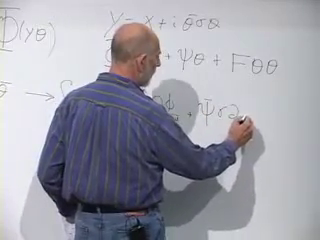
\includegraphics[width=0.76\textwidth]{lecture_09_figure_02.png}\lectureframe{00:27:36.000}\caption{La coordonnée chirale et le développement en composantes, au-dessus des termes du scalaire, du fermion et du champ auxiliaire.}\end{figure}

\section{Ce que sélectionne l’intégrale \texorpdfstring{\(d^2\theta\)}{d2-theta}}

Les interactions et les masses proviennent d’une fonction holomorphe \(W(\Phi)\), le superpotentiel :
\begin{equation}
S_W
=
\int d^4x
\left[
\int d^2\theta\,W(\Phi)
+\mathrm{h.c.}
\right].
\label{eq:l9-superpotential-action}
\end{equation}
Une expression chirale ne dépend pas de manière indépendante de \(\bar\theta\) ; son intégration sur les quatre coordonnées impaires donnerait donc zéro. L’intégrale \(d^2\theta\) sélectionne plutôt sa composante \(\theta^2\).

Pour voir les facteurs combinatoires avant de considérer une fonction générale, prenons \(W(\Phi)=\Phi^n\). Dans
\begin{equation}
(\phi+\sqrt2\,\theta\psi+\theta^2F)^n,
\end{equation}
il existe deux façons d’obtenir exactement deux facteurs \(\theta\). On peut choisir un seul facteur \(F\theta^2\) ou choisir deux facteurs fermioniques.

\begin{classroomqa}\audiencequestion{Combien de termes contiennent un facteur \(F\theta^2\) choisi, et seulement des scalaires par ailleurs : \(n-1\) ou \(n\) ? \lecturetimestamp{00:31:33}}\lecturerresponse{Il y en a \(n\). N’importe lequel des facteurs \(n\) peut fournir \(F\theta^2\) ; les \(n-1\) facteurs restants fournissent \(\phi\). La contribution est \(nF\phi^{n-1}\).}\end{classroomqa}

\begin{classroomqa}\audiencequestion{De combien de façons deux facteurs peuvent-ils fournir les deux fermions ? \lecturetimestamp{00:32:26}}\lecturerresponse{Il y a \(\binom n2=n(n-1)/2\) choix sans ordre. La contraction de Grassmann fixe le terme correspondant en \(\psi\psi\).}\end{classroomqa}

Ainsi, dans la notation de la conférence où les coefficients sont omis,
\begin{equation}
\int d^2\theta\,\Phi^n+\mathrm{h.c.}
\;\leadsto\;
nF\phi^{n-1}
-\frac{n(n-1)}{2}\phi^{n-2}\psi\psi
+\mathrm{h.c.}
\label{eq:l9-power-extraction}
\end{equation}
Le signe moins affiché ici découle du développement normalisé standard et de la convention de Grassmann ; un changement de convention peut modifier les signes apparents.

\begin{classroomqa}\audiencequestion{Qu’est-il advenu du terme \(\phi^n\), qui ne contient aucun facteur \(\theta\) ? \lecturetimestamp{00:33:10}}\lecturerresponse{Il figure bien dans le produit, mais l’intégration \(d^2\theta\) l’élimine. La flèche signifie que l’intégration sélectionne le coefficient de \(\theta^2\) ; elle n’exprime pas l’égalité des expressions complètes.}\end{classroomqa}

\begin{figure}[H]\centering
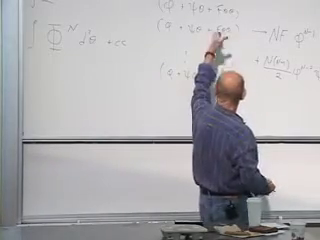
\includegraphics[width=0.82\textwidth]{lecture_09_figure_03.png}\lectureframe{00:33:38.000}\caption{Les facteurs répétés de superchamp et la flèche d’implication, qui extrait la composante en deux facteurs \(\theta\) au lieu de lui être égale.}\end{figure}

La somme des puissances affectées de coefficients arbitraires transforme les facteurs combinatoires en dérivées :
\begin{equation}
\int d^2\theta\,W(\Phi)+\mathrm{h.c.}
\;\leadsto\;
F W'(\phi)
-\frac12 W''(\phi)\psi\psi
+\mathrm{h.c.}
\label{eq:l9-W-components}
\end{equation}

\begin{classroomqa}\audiencequestion{Pourquoi le terme fermionique contient-il \(\phi^{n-2}\) plutôt que \(\phi^{n-1}\) ? \lecturetimestamp{00:36:32}}\lecturerresponse{Deux facteurs ont déjà fourni les fermions ; il reste donc \(n-2\) facteurs scalaires. Le coefficient est la moitié de la dérivée seconde \(W''(\phi)\).}\end{classroomqa}

Le terme fermionique est important : il produit une masse lorsque \(W''\) est constant et une interaction de Yukawa lorsque \(W''\) dépend de \(\phi\). Pour analyser le vide, toutefois, le terme auxiliaire \(FW'\) fournit immédiatement les informations utiles.

\section{Élimination du champ auxiliaire}

Rassemblons les termes qui contiennent \(F\) :
\begin{equation}
\mathcal L_F
=
F^\ast F
+F W'(\phi)
+F^\ast \overline{W'(\phi)}.
\label{eq:l9-LF}
\end{equation}
Comme il n’y a pas de terme \(\partial_\mu F\), l’équation complète d’Euler--Lagrange
\begin{equation}
\partial_\mu
\frac{\partial\mathcal L}{\partial(\partial_\mu F)}
-
\frac{\partial\mathcal L}{\partial F}
=0
\end{equation}
se réduit immédiatement à une équation algébrique. En traitant \(F\) et \(F^\ast\) comme des variables indépendantes, on obtient
\begin{align}
\frac{\partial\mathcal L_F}{\partial F}
&=F^\ast+W'(\phi)=0,
&
\frac{\partial\mathcal L_F}{\partial F^\ast}
&=F+\overline{W'(\phi)}=0,
\label{eq:l9-F-eom}
\end{align}
et donc
\begin{equation}
F^\ast=-W'(\phi),
\qquad
F=-\overline{W'(\phi)}.
\label{eq:l9-F-solution}
\end{equation}

\begin{figure}[H]\centering
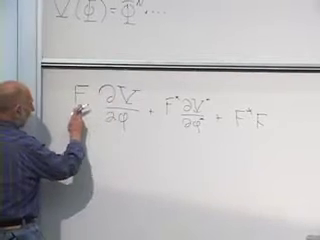
\includegraphics[width=0.82\textwidth]{lecture_09_figure_04.png}\lectureframe{00:39:40.000}\caption{L’expression complète faisant intervenir le champ auxiliaire et son équation du mouvement algébrique, visibles ensemble une fois le tableau dégagé.}\end{figure}

\begin{classroomqa}\audiencequestion{Cette dérivée ne devrait-elle pas être prise par rapport à \(\phi\), plutôt qu’au champ conjugué indiqué au tableau ? \lecturetimestamp{00:41:21}}\lecturerresponse{Oui. La correction rétablit la paire de champs conjugués dans l’équation~\eqref{eq:l9-F-eom} : \(F^\ast=-W'(\phi)\) et \(F=-\overline{W'(\phi)}\).}\end{classroomqa}

La substitution dans l’équation~\eqref{eq:l9-LF} donne
\begin{equation}
\mathcal L_F\big|_{\mathrm{on\ shell}}
=-|W'(\phi)|^2.
\end{equation}
Comme un lagrangien scalaire est égal à l’énergie cinétique moins l’énergie potentielle, le potentiel scalaire usuel est
\begin{equation}
\boxed{V(\phi,\phi^\ast)=|W'(\phi)|^2\ge0.}
\label{eq:l9-F-potential}
\end{equation}
Ce \(V\) n’est pas le superpotentiel. Nous réservons \(W\) à la fonction holomorphe de l’espace supersymétrique et \(V\) à l’énergie potentielle usuelle.

\subsection{Deux exemples immédiats}

Avec les normalisations conventionnelles exactes,
\begin{equation}
\begin{gathered}
W(\Phi)=\frac12m\Phi^2,\\
W'(\phi)=m\phi,
\qquad V=|m|^2|\phi|^2.
\end{gathered}
\label{eq:l9-quadratic-W}
\end{equation}
Le même terme donne la masse du fermion,
\(-\tfrac12m\psi\psi+\mathrm{h.c.}\)
si bien que les masses du scalaire et du fermion sont égales avant la brisure de la supersymétrie.

Pour
\begin{equation}
W(\Phi)=\frac{g}{3}\Phi^3,
\end{equation}
on obtient
\begin{equation}
\begin{gathered}
W'(\phi)=g\phi^2,
\qquad V=|g|^2|\phi|^4,\\
\mathcal L_{\mathrm{Yukawa}}
=-g\phi\psi\psi+\mathrm{h.c.}
\end{gathered}
\label{eq:l9-cubic-W}
\end{equation}
Le vertex scalaire quartique décrit la diffusion de deux scalaires, tandis que le terme de Yukawa en est le partenaire supersymétrique.

\section{Deux types de vide}

Le vide est une configuration de champ constante correspondant à un minimum de \(V\) ; les termes dérivés s’annulent. Comme l’équation~\eqref{eq:l9-F-potential} est non négative, deux cas sont possibles.

\subsection{Un minimum d’énergie nulle}

Si un certain \(\phi_0\) satisfait
\begin{equation}
W'(\phi_0)=0,
\end{equation}
alors
\begin{equation}
V(\phi_0)=0,
\qquad
\langle F\rangle=0.
\label{eq:l9-unbroken-F}
\end{equation}
Le vide est supersymétrique. C’est l’analogue d’une aimantation nulle : aucune composante auxiliaire n’a sélectionné de direction dans l’espace supersymétrique.

\subsection{Un minimum relevé}

Si les équations
\begin{equation}
W'(\phi)=0
\label{eq:l9-F-flatness}
\end{equation}
n’ont pas de solution simultanée au minimum, alors
\begin{equation}
V_{\min}>0,
\qquad
\langle F\rangle\neq0,
\label{eq:l9-broken-F}
\end{equation}
et la supersymétrie est spontanément brisée. L’action demeure supersymétrique ; son état d’énergie minimale, lui, ne l’est pas.

\begin{figure}[H]\centering
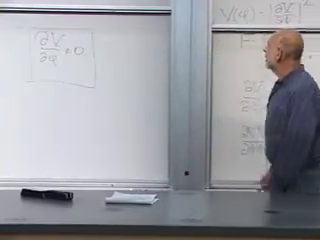
\includegraphics[width=0.88\textwidth]{lecture_09_figure_05.png}\lectureframe{00:52:09.960}\caption{Le tableau présente le potentiel positif, l’équation en \(F\) et la condition sur le vide, tout en distinguant des équations symétriques une solution qui ne l’est pas.}\end{figure}

L’énoncé concernant le paramètre d’ordre se précise à partir de la transformation du fermion :
\begin{equation}
\delta\psi_\alpha
=
i\sqrt2
(\sigma^\mu\bar\epsilon)_\alpha\partial_\mu\phi
+\sqrt2\,\epsilon_\alpha F.
\label{eq:l9-fermion-transformation}
\end{equation}
Dans un vide homogène, le terme dérivé s’annule. Si
\(\langle F\rangle\neq0\), la supersymétrie décale le fermion d’une constante non nulle, de sorte que le vide ne peut pas être invariant.\editorialnote{L’équation~\eqref{eq:l9-fermion-transformation} est la forme standard en composantes qui explicite l’énoncé de la conférence selon lequel les composantes du superchamp se transforment les unes en les autres.}

La même conclusion découle de la superalgèbre. Dans le référentiel au repos,
\begin{equation}
\{Q_\alpha,Q_{\dot\alpha}^\dagger\}
=2\sigma^0_{\alpha\dot\alpha}H.
\end{equation}
La valeur moyenne dans le vide exprime son énergie comme une somme des normes des charges de supersymétrie appliquées au vide :
\begin{equation}
E_0\ge0,
\qquad
E_0=0
\ \Longleftrightarrow\
Q_\alpha|0\rangle
=Q_{\dot\alpha}^\dagger|0\rangle=0.
\label{eq:l9-algebra-vacuum-energy}
\end{equation}
Ainsi, une énergie positive du vide et la brisure spontanée de la supersymétrie sont deux aspects d’un même énoncé en supersymétrie globale.

\begin{center}
\begin{tikzpicture}[x=1.2cm,y=1.0cm,>=Latex]
  \draw[->] (-3,0) -- (-0.2,0) node[right] {\(\phi\)};
  \draw[->] (-2.8,-0.15) -- (-2.8,2.1) node[above] {\(V\)};
  \draw[thick,teal!75!black,domain=-2.5:-0.5,samples=60]
    plot (\x,{0.65*(\x+1.5)^2});
  \fill (-1.5,0) circle (2pt);
  \node[below] at (-1.5,0) {\(F=0\)};
  \draw[->] (0.4,0) -- (3.2,0) node[right] {\(\phi\)};
  \draw[->] (0.6,-0.15) -- (0.6,2.1) node[above] {\(V\)};
  \draw[thick,orange!85!black,domain=0.9:2.9,samples=60]
    plot (\x,{0.55*(\x-1.9)^2+0.65});
  \fill (1.9,0.65) circle (2pt);
  \draw[dashed] (0.6,0.65) -- (1.9,0.65);
  \node[below] at (1.9,0.65) {\(F\neq0\)};
\end{tikzpicture}
\end{center}

\editorialnote{Une illustration minimale est donnée par \(W=f\Phi\), pour laquelle \(W'=f\) ne s’annule jamais et \(V=|f|^2\). Cet exemple à un seul champ présente une direction scalaire plate ; en pratique, la brisure stable par terme \(F\) se réalise généralement au moyen de plusieurs champs chiraux, comme dans les secteurs cachés de type O’Raifeartaigh.}

\section{Ce que produit la brisure de la supersymétrie}

\subsection{Séparation des masses}

L’analogie avec le ferromagnétique redevient spectrale. Un faible champ magnétique interne sépare les niveaux atomiques sans détruire l’identité de l’atome. De même, un paramètre d’ordre associé à la brisure de la supersymétrie, transmis par couplage faible, sépare les bosons et les fermions qui appartiendraient autrement à un même supermultiplet.

\begin{classroomqa}\audiencequestion{Quelles particules la supersymétrie transforme-t-elle les unes en les autres et perdent ainsi leur dégénérescence de masse lorsque le vide brise cette symétrie ? \lecturetimestamp{00:51:40}}\lecturerresponse{Les bosons et les fermions. Leurs masses n’ont plus besoin d’être égales dès lors que l’état ne respecte plus la transformation qui les relie.}\end{classroomqa}

La séparation n’est pas produite par \(\langle F\rangle\) à lui seul ; elle dépend des couplages qui transmettent la brisure aux champs visibles. Si ces couplages sont faibles, les particules visibles restent reconnaissables et les écarts de masse sont petits devant les échelles de grande unification ou de Planck. S’ils étaient forts, l’analogie serait celle d’un atome tellement déformé par un champ magnétique immense qu’il deviendrait un objet allongé et méconnaissable.

\subsection{Le goldstino}

Pour un générateur ordinaire brisé, \(J|0\rangle\) donne un état de Goldstone bosonique. Une charge de supersymétrie est fermionique et transforme les états bosoniques en états fermioniques. Puisque le vide est compté comme bosonique, une charge de supersymétrie brisée crée un état fermionique d’énergie nulle :
\begin{equation}
Q_\alpha|0\rangle
\sim
|\widetilde G_\alpha,\mathbf k=0\rangle.
\label{eq:l9-goldstino}
\end{equation}
La particule correspondante en propagation est un fermion de Weyl sans masse, le fermion de Goldstone, ou goldstino.

\begin{classroomqa}\audiencequestion{Si une transformation supersymétrique ne laisse pas le vide inchangé, quel nouvel état crée-t-elle ? \lecturetimestamp{00:53:24}}\lecturerresponse{Un fermion sans masse. Le schéma du théorème de Goldstone ordinaire subsiste, mais un générateur fermionique transforme le vide bosonique en goldstino.}\end{classroomqa}

La brisure spontanée d’une supersymétrie globale a donc deux signatures inévitables :
\begin{equation}
\boxed{
V_{\min}>0
\qquad\text{and}\qquad
\text{a massless goldstino}.
}
\label{eq:l9-rigid-breaking-signatures}
\end{equation}

\section{Le secteur caché}

Il est utile de considérer l’atome et le ferromagnétique comme deux secteurs. Le ferromagnétique développe le paramètre d’ordre ; l’atome ne ressent que le champ qui lui est transmis. Lorsque le couplage est faible, manipuler l’atome excite à peine un magnon et donne peu d’accès direct au milieu magnétique. Le ferromagnétique est alors caché, même si sa présence se déduit de faibles écarts spectraux.

La construction de modèles supersymétriques reprend le même vocabulaire. Des champs supplémentaires d’un secteur caché développent des valeurs moyennes non nulles des termes \(F\) ou \(D\). Des interactions, dites mécanisme de médiation, transmettent cette brisure au secteur visible et engendrent des masses molles pour les partenaires supersymétriques. Une transmission faible explique comment la théorie visible peut rester approximativement supersymétrique à une échelle fondamentale bien plus élevée, tout en ne présentant aucune dégénérescence exacte entre bosons--fermions à basse énergie.

Cette construction ne se fait pas automatiquement. Il faut des champs supplémentaires, un vide de brisure stable et un mécanisme de médiation contrôlé. C’est pourquoi la conférence décrit la brisure réaliste de la supersymétrie comme compliquée et quelque peu artificielle, plutôt que comme une conséquence unique et inévitable du modèle minimal.

\section{La gravité modifie les deux signatures}

\subsection{L’énergie du vide devient une source}

En l’absence de gravité, ajouter une constante à toutes les énergies ne modifie pas les expériences non gravitationnelles. En présence de gravité, une densité d’énergie du vide intervient dans l’équation d’Einstein comme constante cosmologique. Un \(V_{\min}\) positif entraîne une expansion accélérée. Si son échelle était comparable à celle de la physique des particules requise pour les masses des partenaires supersymétriques, la courbure qui en résulterait serait immensément supérieure à celle qui est observée.

\begin{classroomqa}\audiencequestion{Que fait au monde une énergie du vide positive et non nulle lorsque l’on tient compte de la gravité ? \lecturetimestamp{01:00:40}}\lecturerresponse{Elle agit comme une constante cosmologique et entraîne une expansion accélérée. Aux échelles usuelles de la physique des particules, son effet serait intolérablement important.}\end{classroomqa}

La supersymétrie locale, ou supergravité, modifie la formule exprimant le potentiel comme un carré positif. Pour fixer les idées, le potentiel standard associé aux termes \(N=1\) \(F\) s’écrit
\begin{equation}
\begin{aligned}
V_F={}&e^{K/M_P^2}
\left(
K^{i\bar j}D_iW\,D_{\bar j}\overline W
-\frac{3|W|^2}{M_P^2}
\right),\\
D_iW={}&\partial_iW+\frac{\partial_iK}{M_P^2}W.
\end{aligned}
\label{eq:l9-sugra-potential}
\end{equation}
En raison du terme négatif, l’énergie positive due à la brisure de la supersymétrie peut en principe être partiellement compensée. Le résidu peut correspondre à une faible constante cosmologique.

\editorialnote{La conférence ne donne volontairement qu’une correction schématique et met explicitement en doute la position de la masse de Planck. L’équation~\eqref{eq:l9-sugra-potential} donne la formule conventionnelle pour des multiplets chiraux de potentiel de Kähler \(K\) ; les termes de jauge \(D\) ajouteraient une contribution supplémentaire non négative. Elle n’explique pas la valeur infime observée, qui reste le problème de la constante cosmologique.}

\subsection{Le mécanisme super-Higgs}

Le second effet gravitationnel se comprend le plus facilement en comptant les polarisations. Une particule massive de spin-\(j\) possède \(2j+1\) états de spin dans son référentiel au repos.

\begin{classroomqa}\audiencequestion{Combien d’états de spin possède une particule massive de spin-\(j\) ? \lecturetimestamp{01:05:16}}\lecturerresponse{\(2j+1\). Une particule massive de spin un possède notamment trois états, tandis qu’un boson de jauge sans masse n’a que les hélicités \(+1\) et \(-1\).}\end{classroomqa}

La distinction est cinématique. On peut appliquer un boost à une particule massive pour la mettre au repos, puis la diriger dans une nouvelle direction tout en conservant l’orientation de son spin ; toutes les projections doivent donc exister. Une particule sans masse ne peut être dépassée ni mise au repos. Elle ne peut donc porter que les deux hélicités extrêmes.

Pour le champ de jauge électrofaible,
\begin{equation}
\underbrace{(+1,-1)}_{\text{massless vector}}
+
\underbrace{(0)}_{\text{Goldstone}}
\longrightarrow
\underbrace{(+1,0,-1)}_{\text{massive vector}}.
\label{eq:l9-higgs-count}
\end{equation}

\begin{classroomqa}\audiencequestion{D’où vient la polarisation longitudinale d’un \(W\) ou d’un \(Z\) massif ? \lecturetimestamp{01:08:50}}\lecturerresponse{Du boson de Goldstone. Il est absorbé par le champ de jauge et complète la représentation massive de spin un, qui comporte trois états.}\end{classroomqa}

La gravité possède un graviton sans masse de spin deux. Son partenaire supersymétrique est le gravitino sans masse de spin-\(\tfrac32\).

\begin{classroomqa}\audiencequestion{Quel est le spin du graviton et, par conséquent, celui de son partenaire supersymétrique ? \lecturetimestamp{01:10:24}}\lecturerresponse{Le graviton a un spin \(2\) ; son partenaire fermionique diffère d’une demi-unité et a un spin \(3/2\).}\end{classroomqa}

Un gravitino sans masse a les hélicités \(\pm\tfrac32\), tandis qu’un gravitino massif doit aussi posséder \(\pm\tfrac12\). Le goldstino fournit précisément ces états manquants :
\begin{equation}
\begin{gathered}
\underbrace{\left(+\frac32,-\frac32\right)}_{\text{massless gravitino}}
\oplus
\underbrace{\left(+\frac12,-\frac12\right)}_{\text{goldstino}}\\
\Downarrow\\
\underbrace{\left(+\frac32,+\frac12,-\frac12,-\frac32\right)}_{\text{massive gravitino}}.
\end{gathered}
\label{eq:l9-super-higgs}
\end{equation}
C’est le mécanisme super-Higgs. Lorsque la supersymétrie est locale, le goldstino est absorbé et n’apparaît plus comme particule sans masse indépendante. Le gravitino qui en résulte interagit par gravitation et est donc difficile à produire.

\section{Changement de sujet : pourquoi \texorpdfstring{\(SU(5)\)}{SU(5)}}

Le formalisme de la supersymétrie cède maintenant la place à la grande unification. Le groupe de jauge du Modèle standard est
\begin{equation}
G_{\mathrm{SM}}
=SU(3)_c\times SU(2)_L\times U(1)_Y.
\label{eq:l9-sm-group}
\end{equation}
Ses trois facteurs organisent séparément la couleur, l’isospin faible et l’hypercharge faible. La question de l’unification est de savoir si ce produit est un sous-groupe survivant d’un groupe simple plus grand, de sorte que les multiplets de particules et les forces de jauge apparemment distincts soient les éléments d’une structure unique. Le candidat minimal étudié ici est \(SU(5)\).

\subsection{Éléments et générateurs du groupe}

Pour \(U\in SU(N)\),
\begin{equation}
U^\dagger U=\mathbf1,
\qquad
\det U=1.
\label{eq:l9-SUN-def}
\end{equation}
La première condition exprime l’unitarité ; la seconde définit le caractère spécial du groupe. Écrivons un élément infinitésimal sous la forme
\begin{equation}
U=\mathbf1+i\epsilon G+\mathcal O(\epsilon^2).
\label{eq:l9-infinitesimal-U}
\end{equation}
L’unitarité impose
\begin{equation}
G^\dagger=G,
\end{equation}
et
\begin{equation}
\det e^{i\epsilon G}
=e^{i\epsilon\operatorname{tr}G}=1
\end{equation}
impose
\begin{equation}
\operatorname{tr}G=0.
\end{equation}
Les générateurs sont donc des matrices hermitiennes sans trace.

Une matrice hermitienne \(N\times N\) contient \(N^2\) paramètres réels : \(N\) entrées diagonales réelles et \(N(N-1)/2\) entrées hors diagonale complexes. La condition de trace nulle en élimine un. On a donc
\begin{equation}
\dim SU(N)=N^2-1,
\qquad
\dim SU(5)=24.
\label{eq:l9-SU5-dimension}
\end{equation}
À titre de comparaison, \(SU(2)\) possède trois générateurs de Pauli et \(SU(3)\) huit générateurs de couleur.

\section{Les blocs du Modèle standard dans \texorpdfstring{\(SU(5)\)}{SU(5)}}

Partageons l’espace de dimension cinq en un bloc faible de dimension deux et un bloc de couleur de dimension trois :
\begin{equation}
\mathbf5=\mathbf2\oplus\mathbf3.
\end{equation}
Les générateurs plongés dans ces blocs ont la forme
\begin{align}
T^a_L
&=
\begin{pmatrix}
\tfrac12\tau^a&0\\
0&0_{3\times3}
\end{pmatrix},
&& a=1,2,3,
\label{eq:l9-SU2-block}\\
T^A_c
&=
\begin{pmatrix}
0_{2\times2}&0\\
0&\tfrac12\lambda^A
\end{pmatrix},
&& A=1,\ldots,8.
\label{eq:l9-SU3-block}
\end{align}
Les matrices de Pauli \(\tau^a\) engendrent le groupe faible \(SU(2)\) ; les matrices de Gell-Mann \(\lambda^A\) engendrent le groupe de couleur \(SU(3)\). Comme les blocs ne se recouvrent pas, les deux sous-groupes commutent.

Un générateur diagonal supplémentaire est proportionnel à l’identité dans chaque bloc et commute donc avec les deux. Dans la représentation fondamentale, une convention pratique pour l’hypercharge, multipliée par deux, est
\begin{equation}
T_Y^{(\mathbf5)}=
\operatorname{diag}
\left(
1,1,-\frac23,-\frac23,-\frac23
\right).
\label{eq:l9-hypercharge-generator}
\end{equation}
Sa trace est nulle :
\begin{equation}
1+1-3\left(\frac23\right)=0.
\end{equation}
La représentation conjuguée de matière a les valeurs propres opposées,
\begin{equation}
Y_{\overline{\mathbf5}}
=
\operatorname{diag}
\left(
-1,-1,\frac23,\frac23,\frac23
\right),
\label{eq:l9-fivebar-hypercharge}
\end{equation}
qui sont les valeurs indiquées pour la colonne de matière dans la conférence. Le signe global et la normalisation sont conventionnels ; ces entrées suivent la convention du Modèle standard
\begin{equation}
Q=T_3+\frac{Y}{2}.
\label{eq:l9-charge}
\end{equation}
Les équations~\eqref{eq:l9-SU2-block}--\eqref{eq:l9-hypercharge-generator} affichent
\begin{equation}
SU(3)_c\times SU(2)_L\times U(1)_Y
\subset SU(5).
\end{equation}

Les 3 générateurs faibles, les 8 générateurs de couleur et le générateur d’hypercharge représentent \(12\) des \(24\) générateurs de \(SU(5)\).\editorialnote{Les 12 autres occupent les blocs hors diagonale \(2\times3\) et \(3\times2\). Les bosons de jauge correspondants convertissent les composantes de type quark en composantes de type lepton, et inversement ; c’est là l’origine structurelle des interactions qui changent le nombre baryonique et le nombre leptonique, développées dans la suite.}

\begin{classroomqa}
\audiencequestion{Quelles particules de jauge correspondent aux générateurs du sous-groupe familier ? \lecturetimestamp{01:31:05}}
\lecturerresponse{Les 8 générateurs de \(SU(3)\) donnent les 8 gluons. Les 3 générateurs de \(SU(2)\) donnent les champs de jauge faibles, qui, après le mélange électrofaible, deviennent \(W^\pm\) et une partie du système \(Z\)-photon ; le champ \(U(1)\) fournit l’autre combinaison neutre.}
\end{classroomqa}

\section{Une famille exprimée en champs gauches}

Considérons la première génération ; le même schéma se répète pour les générations muon/charm/étrange et tau/top/bottom. Le plus simple est de compter chaque champ de Weyl indépendant comme un champ gauche. Les particules droites sont représentées par leurs champs conjugués de charge gauches :
\begin{equation}
Q_L=(u_L,d_L),\quad
L_L=(\nu_{eL},e_L),\quad
u^c_L,\quad d^c_L,\quad e^c_L.
\end{equation}
Leurs multiplicités sont
\begin{equation}
\underbrace{6}_{Q_L}
+
\underbrace{2}_{L_L}
+
\underbrace{3}_{u^c_L}
+
\underbrace{3}_{d^c_L}
+
\underbrace{1}_{e^c_L}
=15.
\label{eq:l9-fifteen-fields}
\end{equation}

\editorialnote{Le modèle standard minimal ne contient aucun champ de Weyl indépendant de neutrino droit ; le décompte est donc \(15\). Ce décompte, à lui seul, n’affirme pas que le neutrino est une particule de Majorana. L’ajout d’un singulet \(\nu^c_L\) porte le nombre de champs à \(16\) et conduit naturellement vers \(SO(10)\), au-delà de la construction \(SU(5)\) considérée ici.}

Le multiplet de dimension cinq doit placer les composantes de doublet faible sans couleur dans les deux premières positions, et les singulets faibles colorés dans les trois dernières.

\begin{classroomqa}
\audiencequestion{La colonne proposée contient-elle six champs au lieu de cinq ? \lecturetimestamp{01:36:14}}
\lecturerresponse{Non. Le quark up écrit dans un premier temps est effacé. La colonne contient le neutrino, l’électron et trois copies de couleur de l’antiquark down : cinq composantes en tout.}
\end{classroomqa}

On obtient
\begin{equation}
\overline{\mathbf5}
=
\begin{pmatrix}
\nu_{eL}\\
e_L\\
d^c_{rL}\\
d^c_{gL}\\
d^c_{bL}
\end{pmatrix}.
\label{eq:l9-fivebar}
\end{equation}
\editorialnote{Dans la notation standard où tous les champs sont gauches, les affectations de couleur et d’hypercharge identifient ce multiplet, que le cours qualifie d’abord simplement de multiplet de dimension cinq, à la représentation conjuguée \(SU(5)\) \(\overline{\mathbf5}\).}
Les deux premières composantes se transforment sous \(SU(2)_L\), mais ne portent pas de couleur. Les trois dernières se transforment comme un antitriplet de couleur, mais sont des singulets faibles.

\begin{classroomqa}
\audiencequestion{Quels quarks portent la couleur, mais aucun nombre quantique faible \(SU(2)_L\), lorsque tous les champs sont écrits comme des champs gauches ? \lecturetimestamp{01:40:13}}
\lecturerresponse{Les conjugués de charge des quarks droits. Pour ce multiplet à cinq composantes, le critère de charge sélectionne les trois champs d’antiquark down \(d^c_{r,g,b}\).}
\end{classroomqa}

Les charges électriques dans l’équation~\eqref{eq:l9-fivebar} ont une somme nulle :
\begin{equation}
0-1+\frac13+\frac13+\frac13=0.
\label{eq:l9-fivebar-charge-sum}
\end{equation}
C’est nécessaire, car l’opérateur de charge électrique est une combinaison sans trace des générateurs de \(SU(5)\).

\begin{classroomqa}
\audiencequestion{Pourquoi les antiquarks down, plutôt que les antiquarks up, occupent-ils les trois positions de couleur ? \lecturetimestamp{01:43:38}}
\lecturerresponse{Le neutrino et l’électron contribuent une charge totale de \(-1\). Les trois couleurs d’antiquark down contribuent \(+1\), ce qui donne une trace nulle. Trois champs d’antiquark up donneraient une charge totale incorrecte.}
\end{classroomqa}

Les 10 champs gauches restants sont
\begin{equation}
Q_L\;(6)
\oplus
u^c_L\;(3)
\oplus
e^c_L\;(1),
\end{equation}
et ils s’insèrent exactement dans la représentation antisymétrique de rang deux
\begin{equation}
\mathbf{10}\cong\wedge^2\mathbf5,
\qquad
\dim\wedge^2\mathbf5=\binom52=10.
\label{eq:l9-ten-preview}
\end{equation}
Leur placement explicite sera l’objet du cours suivant. Cet ajustement numérique
\begin{equation}
\overline{\mathbf5}\oplus\mathbf{10}
\end{equation}
pour chaque famille du modèle standard constitue le premier indice frappant que l’idée de \(SU(5)\) est plus qu’un simple réétiquetage arbitraire.

\begin{classroomqa}
\audiencequestion{Si les représentations cinq et dix sont différentes, cela signifie-t-il que leurs particules ne peuvent pas interagir ? \lecturetimestamp{01:46:14}}
\lecturerresponse{Non. Une transformation de groupe agit au sein de chaque représentation irréductible ; elle ne fait donc pas directement passer un élément du cinq à un élément du dix. Les deux ensembles peuvent néanmoins interagir par émission et absorption de bosons de jauge communs, et les couplages de Higgs peuvent également relier leurs champs.}
\end{classroomqa}

\section{En perspective}

Le cours a suivi un même schéma à des échelles très différentes. L’invariance par rotation rend les niveaux atomiques dégénérés ; un champ magnétique lève cette dégénérescence. Un ferromagnétique produit un tel champ tout en laissant les lois sous-jacentes symétriques, et ses magnons sans gap révèlent que la dissymétrie réside dans le vide. Dans une théorie supersymétrique chirale, la valeur moyenne de l’auxiliaire joue le rôle du paramètre d’ordre :
\begin{equation}
\begin{aligned}
\langle F\rangle=0
&\quad\Longleftrightarrow\quad
\text{unbroken supersymmetry},\\
\langle F\rangle\neq0
&\quad\Longrightarrow\quad
\text{spontaneous breaking}.
\end{aligned}
\end{equation}
Dans la supersymétrie rigide, le vide brisé possède une énergie positive, lève la dégénérescence des supermultiplets et produit un goldstino. La médiation faible motive l’introduction d’un secteur caché ; la gravité transforme l’énergie du vide en problème cosmologique et absorbe le goldstino dans un gravitino massif.

La construction finale en \(SU(5)\) ouvre une nouvelle question au lieu de la résoudre. Les générateurs hermitiens sans trace \(5\times5\) contiennent les blocs du modèle standard, et les cinq premiers champs de matière s’insèrent exactement comme suit :
\((\nu_e,e^-,d^c_r,d^c_g,d^c_b)\). Les dix autres attendent dans la représentation antisymétrique. C’est à partir de cet ajustement encore inachevé que commence véritablement la grande unification.

\chapter{Les multiplets de \texorpdfstring{\(SU(5)\)}{SU(5)}, les bosons de jauge leptoquarks et la désintégration du proton}

\lectureoverview{La grande unification devient concrète lorsque le groupe du Modèle standard est inclus dans \(SU(5)\). Pour comprendre ce que cela signifie, nous commençons par établir les éléments nécessaires de la théorie des représentations : la représentation définissante \(N\), sa conjuguée \(\overline N\), les produits tensoriels, les tenseurs symétriques et antisymétriques, ainsi que la représentation adjointe. Une famille du Modèle standard se regroupe alors dans la combinaison étonnamment économique \(\overline{\mathbf 5}\oplus\mathbf{10}\). La même symétrie qui rend cette organisation élégante impose aussi l’existence de bosons de jauge colorés qui transforment les quarks en leptons. Leur échange permet la désintégration du proton, ce qui contraint l’échelle d’unification à se situer vers \(10^{15}\)--\(10^{16}\,\mathrm{GeV}\). L’évolution des couplages de jauge suggère une échelle comparable, et la supersymétrie revient à la fin, car elle rend leur convergence numérique nettement plus précise.}

\section{Pourquoi commencer par les représentations de groupe ?}

Il existe de nombreuses théories de grande unification proposées. Plutôt que de les passer en revue, nous allons examiner un exemple et poser trois questions : qu’est-ce qui le fait fonctionner, quelles nouvelles particules exige-t-il, et comment les expériences le mettent-elles en difficulté ? Le groupe est \(SU(5)\), et sa caractéristique structurelle essentielle est l’inclusion
\begin{equation}
SU(3)_c\times SU(2)_L\times U(1)_Y
\subset SU(5).
\label{eq:l10-sm-embedding}
\end{equation}
Ici, \(SU(3)_c\) agit sur la couleur, \(SU(2)_L\) sur l’isospin faible et \(U(1)_Y\) sur l’hypercharge.

La supersymétrie n’est pas une prémisse de cette construction. Ni la supersymétrie ni la grande unification n’impliquent logiquement l’autre. Leur lien dans ce cours est numérique : lorsqu’on inclut le spectre des superpartenaires dans le calcul du groupe de renormalisation, les trois couplages de jauge se rapprochent davantage d’une valeur commune.

Les particules qu’une symétrie mélange entre elles forment une représentation du groupe de symétrie. Il faut donc d’abord quelques notions de théorie des représentations pour classer les multiplets de particules unifiées.

\subsection{L’exemple familier de \texorpdfstring{\(SU(2)\)}{SU(2)}}

Le groupe \(SU(2)\) associé au moment cinétique ordinaire est étroitement lié aux rotations de l’espace tridimensionnel. Plus précisément, \(SU(2)\) est le revêtement double de \(SO(3)\). Ses représentations irréductibles sont indexées par
\begin{equation}
j=0,\frac12,1,\frac32,\ldots,
\qquad
\dim(j)=2j+1.
\label{eq:l10-su2-spins}
\end{equation}
Ainsi, un scalaire est un singulet, une particule de spin \(\tfrac12\) est un doublet et une particule de spin un est un triplet. Le groupe faible \(SU(2)_L\) est une symétrie physique différente, bien que sa théorie des groupes abstraite soit la même.

\section{La représentation définissante et sa conjuguée}

Pour \(SU(N)\), la représentation définissante est l’espace des colonnes complexes à \(N\) composantes,
\begin{equation}
\psi=
\begin{pmatrix}
\psi_1\\
\psi_2\\
\vdots\\
\psi_N
\end{pmatrix},
\qquad
\psi'_i=U_i{}^j\psi_j,
\qquad
U\in SU(N).
\label{eq:l10-defining}
\end{equation}
On l’appelle représentation définissante ou, plus simplement, \(\mathbf N\). Les matrices \(U\) sont de taille \(N\times N\), et l’espace vectoriel sur lequel elles agissent est de dimension \(N\).

La conjugaison complexe fournit une autre représentation de dimension \(N\),
\begin{equation}
\psi_i^*\longmapsto U_i{}^{j*}\psi_j^*,
\label{eq:l10-conjugate}
\end{equation}
notée \(\overline{\mathbf N}\). Pour \(N>2\), les représentations définissante et conjuguée ne sont pas équivalentes. On peut intervertir les appellations de représentation des particules et des antiparticules, mais une fois la convention choisie, il faut la conserver.

\begin{classroomqa}
\audiencequestion{Le \(N\) dans \(SU(N)\) dépend-il du fait que \(N\) soit pair ou impair, et désigne-t-il les matrices ? \lecturetimestamp{00:07:33}}
\lecturerresponse{Il n’y a ici aucune restriction de parité --. \(N\) désigne la taille des matrices définissantes et aussi la dimension de leur représentation définissante. \(\mathbf N\) et \(\overline{\mathbf N}\) ont toutes deux cette dimension.}
\end{classroomqa}

L’antiparticule d’une antiparticule est la particule initiale. C’est pourquoi intervertir les appellations \(\mathbf N\) et \(\overline{\mathbf N}\) revient à changer de convention, et non de physique.

\section{Produits tensoriels et irréductibilité}

Supposons qu’un objet puisse occuper \(N\) états internes et qu’un autre puisse indépendamment en occuper autant. Si l’on fait abstraction de la position, de la quantité de mouvement, du spin et de tous les nombres quantiques à l’exception de cet indice \(SU(N)\), la paire possède
\begin{equation}
N\times N=N^2
\label{eq:l10-product-count}
\end{equation}
états. Si le premier objet est dans l’état \(\psi_i\) et le second dans l’état \(\phi_j\), leur produit peut s’écrire
\begin{equation}
\Psi_{ij}=\psi_i\phi_j,
\qquad
\Psi'_{ij}=U_i{}^kU_j{}^\ell\Psi_{k\ell}.
\label{eq:l10-tensor-transform}
\end{equation}
C’est le produit tensoriel \(\mathbf N\otimes\mathbf N\).

\begin{classroomqa}
\audiencequestion{Pourquoi obtient-on \(N^2\) plutôt que \(N^2-1\), et le fait d’autoriser les deux particules à avoir le même indice interne viole-t-il le principe d’exclusion ? \lecturetimestamp{00:10:22}}
\lecturerresponse{Les deux emplacements sont ici distinguables : un objet est fixé à une position et l’autre à une autre. Le principe de Pauli porte sur l’état quantique complet, position comprise. Il n’élimine aucune de ces \(N^2\) combinaisons d’indices internes. Le nombre \(N^2-1\) apparaîtra plus tard, à la suite d’une condition de trace nulle dans un autre produit.}
\end{classroomqa}

La représentation produit de dimension \(N^2\) est en général réductible. Une représentation est réductible lorsqu’elle contient un sous-espace propre que le groupe laisse invariant. On peut isoler ces sous-espaces invariants et les traiter comme des représentations plus petites ; en l’absence d’un tel sous-espace propre, la représentation est irréductible.

\subsection{Tenseurs symétriques et antisymétriques}

Tout tenseur à deux indices se décompose de manière unique en
\begin{align}
\Psi_{ij}
&=\Psi^{(S)}_{ij}+\Psi^{(A)}_{ij},\\
\Psi^{(S)}_{ij}
&=\frac12(\Psi_{ij}+\Psi_{ji}),\\
\Psi^{(A)}_{ij}
&=\frac12(\Psi_{ij}-\Psi_{ji}).
\label{eq:l10-sym-anti}
\end{align}
Les deux termes vérifient
\begin{equation}
\Psi^{(S)}_{ij}=\Psi^{(S)}_{ji},
\qquad
\Psi^{(A)}_{ij}=-\Psi^{(A)}_{ji}.
\end{equation}
L’équation~\eqref{eq:l10-tensor-transform} préserve chacune de ces conditions : les transformations du groupe ne mélangent donc jamais les secteurs symétrique et antisymétrique.

\editorialnote{Le cours laisse le dénombrement général en exercice. Les dimensions des secteurs symétrique et antisymétrique sont respectivement \(N(N+1)/2\) et \(N(N-1)/2\), et leur somme vaut \(N^2\).}

\begin{figure}[htbp]
\centering
\includegraphics[width=0.78\textwidth]{lecture_10_figure_02.png}
\lectureframe{00:17:57.500}
\caption{La décomposition complète au tableau des états de spin \(\tfrac12\) : trois états symétriques et un état antisymétrique.}
\label{fig:l10-spin-decomposition}
\end{figure}

Pour le doublet définissant de \(SU(2)\),
\begin{equation}
\mathbf2\otimes\mathbf2=\mathbf3_S\oplus\mathbf1_A.
\label{eq:l10-two-two}
\end{equation}
En notant les deux états de base \(u\) et \(d\), le triplet symétrique est
\begin{align}
\ket{1,1}&=\ket{uu},\\
\ket{1,0}&=\frac{1}{\sqrt2}\bigl(\ket{ud}+\ket{du}\bigr),\\
\ket{1,-1}&=\ket{dd},
\end{align}
tandis que le singulet antisymétrique est
\begin{equation}
\ket{0,0}
=\frac{1}{\sqrt2}\bigl(\ket{ud}-\ket{du}\bigr).
\end{equation}
C’est l’addition familière de deux moments cinétiques de spin \(\tfrac12\) : les quatre états bruts se réorganisent en un état de spin un et un état de spin zéro.

\section{Une particule et une antiparticule : la représentation adjointe}

Combinons maintenant la représentation définissante avec sa conjuguée. Le produit comporte toujours \(N^2\) composantes, mais se transforme comme une matrice :
\begin{equation}
M_i{}^j\in\mathbf N\otimes\overline{\mathbf N},
\qquad
M\longmapsto U M U^\dagger.
\label{eq:l10-matrix-transform}
\end{equation}
Contrairement à \(\mathbf N\otimes\mathbf N\), il n’y a pas de symétrie d’échange pertinente entre un indice fondamental et un indice antifondamental. La décomposition naturelle est plutôt
\begin{equation}
M
=
\frac{\operatorname{tr}M}{N}\,\mathbf1_N
+
\left(M-\frac{\operatorname{tr}M}{N}\,\mathbf1_N\right).
\label{eq:l10-trace-split}
\end{equation}
Le premier terme est un singulet et la partie sans trace est la représentation adjointe :
\begin{equation}
\mathbf N\otimes\overline{\mathbf N}
=\mathbf1\oplus\mathbf{Adj},
\qquad
\dim\mathbf{Adj}=N^2-1.
\label{eq:l10-adjoint}
\end{equation}

\begin{figure}[htbp]
\centering
\includegraphics[width=0.67\textwidth]{lecture_10_figure_04.png}
\lectureframe{00:23:47.500}
\caption{Conclusion au tableau pour \(\mathbf N\otimes\overline{\mathbf N}\) : ses \(N^2-1\) composantes sans trace forment la représentation adjointe.}
\label{fig:l10-adjoint}
\end{figure}

Pour \(SU(3)\), on obtient l’octet familier,
\begin{equation}
\mathbf3\otimes\overline{\mathbf3}
=\mathbf8\oplus\mathbf1,
\end{equation}
et les huit gluons se transforment selon la représentation adjointe. Pour \(SU(2)\), la représentation adjointe est de dimension trois et se transforme comme un spin un.

\section{Une famille du Modèle standard}

On observe trois générations, mais \(SU(5)\) reproduit la même construction séparément pour chacune. Il n’explique pas pourquoi il y a trois copies. Nous nous concentrons donc sur la première génération.

Tous les champs seront écrits comme des champs de Weyl gauches. Un fermion droit est représenté par son champ conjugué de charge gauche :
\begin{equation}
u^c_L,\qquad d^c_L,\qquad e^c_L.
\label{eq:l10-left-handed-bookkeeping}
\end{equation}
L’exposant \(c\) indique la conjugaison de charge ; par exemple, \(d^c_L\) est un champ anti-down gauche de charge électrique \(+\tfrac13\).

Dans la notation standard de \(SU(5)\), cinq des quinze champs gauches s’insèrent dans
\begin{equation}
\overline{\mathbf5}
=
\begin{pmatrix}
\nu_{eL}\\
e_L\\
d^c_{rL}\\
d^c_{gL}\\
d^c_{bL}
\end{pmatrix}.
\label{eq:l10-fivebar}
\end{equation}
L’ordre choisi place un bloc faible à deux dimensions avant un bloc de couleur à trois dimensions. Les transformations faibles mélangent les deux premières composantes, les transformations de couleur mélangent les trois dernières, et les générateurs \(SU(5)\) hors diagonale relient les deux blocs.

\editorialnote{Dans l’équation~\eqref{eq:l10-fivebar}, le cours appelle la colonne un \(\mathbf5\), puis désigne le multiplet antisymétrique comme un \(\overline{\mathbf{10}}\). Il s’agit de la convention globalement conjuguée. Nous adoptons la convention standard moderne \(\overline{\mathbf5}\oplus\mathbf{10}\) ; conjuguer toutes les représentations permet de retrouver les appellations du cours sans en modifier la physique.}

L’inventaire minimal complet de la première génération est
\begin{equation}
\begin{gathered}
\underbrace{Q_L=(u_L,d_L)}_{6}
\oplus
\underbrace{L_L=(\nu_{eL},e_L)}_{2},\\
\underbrace{u^c_L}_{3}
\oplus
\underbrace{d^c_L}_{3}
\oplus
\underbrace{e^c_L}_{1},\\
6+2+3+3+1=15.
\end{gathered}
\label{eq:l10-fifteen}
\end{equation}
Le Modèle standard minimal ne comporte pas de \(\nu^c_L\) indépendant et ne donne donc aucune masse de neutrino renormalisable. Les oscillations des neutrinos montrent que cette description minimale est incomplète : la nature possède de petites masses de neutrinos non nulles et une extension est nécessaire.

\begin{classroomqa}
\audiencequestion{Lorsqu’une masse fermionique transforme un état gauche en état droit, transforme-t-elle aussi la particule en son antiparticule ? \lecturetimestamp{00:34:00}}
\lecturerresponse{Non. La masse de l’électron relie un électron gauche à un électron droit de même charge électrique. Dans la notation où tous les champs sont gauches, le second champ est représenté par \(e^c_L\), mais la particule à quatre composantes reste un électron. Seul un champ neutre peut avoir une masse de Majorana qui identifie la particule à son antiparticule.}
\end{classroomqa}

\section{Les bosons de jauge que l’on reconnaît dans le quintuplet}

À chaque générateur d’une symétrie de jauge est associé un champ de jauge. Dans ~\eqref{eq:l10-fivebar}, les transitions familières sont déjà reconnaissables :
\begin{itemize}
\item les champs de jauge faibles agissent entre \(\nu_{eL}\) et \(e_L\) ;
\item les gluons agissent entre les trois couleurs de \(d^c_L\) ;
\item les générateurs neutres agissent diagonalement ;
\item de nouveaux générateurs hors diagonale transforment une composante leptonique en composante colorée, ou inversement.
\end{itemize}

On peut se représenter le gluon comme porteur des nombres quantiques de couleur d’un quark--antiquark. Le cours utilise le moyen mnémotechnique habituel des lignes d’univers : si l’on suit à rebours l’antiquark sortant à travers le sommet d’émission, il ressemble à un quark qui avance. Le champ émis porte donc les nombres quantiques d’une paire quark--antiquark. Dans le langage des représentations, c’est précisément la partie sans trace de \(\mathbf3\otimes\overline{\mathbf3}\).

Pour \(SU(5)\),
\begin{equation}
\dim\mathbf{Adj}_{SU(5)}=5^2-1=24.
\end{equation}
La décomposition de ces champs de jauge sous le sous-groupe du Modèle standard est
\begin{equation}
\mathbf{24}
=
(\mathbf8,\mathbf1)_0
\oplus(\mathbf1,\mathbf3)_0
\oplus(\mathbf1,\mathbf1)_0
\oplus(\mathbf3,\mathbf2)_{-5/6}
\oplus(\overline{\mathbf3},\mathbf2)_{5/6},
\label{eq:l10-adjoint-sm}
\end{equation}
où la paire ordonnée désigne \(SU(3)_c\times SU(2)_L\) et l’indice inférieur est l’hypercharge.

\editorialnote{L’équation~\eqref{eq:l10-adjoint-sm} explicite la structure en blocs dessinée dans le cours. Les trois premiers termes contiennent les champs de jauge familiers de couleur et d’interaction électrofaible. Les deux derniers correspondent aux douze degrés de liberté réels que l’on appelle conventionnellement les bosons \(X\) et \(Y\).}

\begin{figure}[htbp]
\centering
\begin{tikzpicture}[x=1.05cm,y=0.82cm]
  \draw[thick] (0,0) rectangle (5,5);
  \draw[thick] (2,0) -- (2,5);
  \draw[thick] (0,3) -- (5,3);
  \fill[blue!9] (0,3) rectangle (2,5);
  \fill[orange!10] (2,0) rectangle (5,3);
  \fill[teal!9] (2,3) rectangle (5,5);
  \fill[teal!9] (0,0) rectangle (2,3);
  \node[align=center] at (1,4) {weak and\\neutral fields};
  \node[align=center] at (3.5,1.5) {gluons and\\neutral field};
  \node[align=center] at (3.5,4) {\(X,Y\)};
  \node[align=center] at (1,1.5) {\(\overline X,\overline Y\)};
  \node[above] at (1,5) {\(2\)};
  \node[above] at (3.5,5) {\(3\)};
\end{tikzpicture}
\caption{Structure en blocs \(2\oplus3\) du champ de jauge de \(SU(5)\). Les blocs hors diagonale relient les leptons aux champs colorés.}
\label{fig:l10-gauge-blocks}
\end{figure}

Avec la convention \(Q=T_3+Y\), le doublet faible coloré dans ~\eqref{eq:l10-adjoint-sm} porte les charges \(-\tfrac13\) et \(-\tfrac43\) ; son conjugué porte les charges \(+\tfrac13\) et \(+\tfrac43\). Le cours appelle ces particules \(X\) et \(Y\), mais s’abstient explicitement de préciser quelle appellation correspond à quelle charge. La transition et la charge constituent le contenu invariant.

\begin{classroomqa}
\audiencequestion{Existe-t-il trois versions de chaque nouveau boson de jauge \(X\) ou \(Y\) ? \lecturetimestamp{00:41:28}}
\lecturerresponse{Oui. Une transition relie une composante de quark colorée à une composante leptonique sans couleur ; le boson échangé doit donc porter la couleur manquante. Les champs \(X/Y\) forment des triplets de couleur et peuvent émettre ou absorber des gluons.}
\end{classroomqa}

On n’observe pas de particules colorées comme états asymptotiques isolés. Les nouveaux bosons de jauge doivent se désintégrer ou hadroniser en combinaisons neutres en couleur, comme les quarks.

\section{Pourquoi le multiplet contient des quarks anti-down}

Les générateurs de \(SU(N)\) sont des matrices hermitiennes de trace nulle. Pour voir le lien avec le terme « spécial », écrivons un élément infinitésimal du groupe sous la forme
\begin{equation}
U(\epsilon)=e^{i\epsilon T}.
\end{equation}
L’unitarité donne \(T^\dagger=T\), tandis que
\begin{equation}
1=\det U=e^{i\epsilon\operatorname{tr}T}
\end{equation}
pour tout \(\epsilon\) donne
\begin{equation}
\operatorname{tr}T=0.
\label{eq:l10-traceless-generator}
\end{equation}

La charge électrique est une combinaison linéaire de générateurs. Sur la colonne de matière de ~\eqref{eq:l10-fivebar}, elle agit comme suit :
\begin{equation}
Q_{\overline5}
=
\operatorname{diag}
\left(0,-1,\frac13,\frac13,\frac13\right),
\qquad
\operatorname{tr}Q_{\overline5}=0.
\label{eq:l10-charge-fivebar}
\end{equation}
On a donc
\begin{equation}
0-1+3\left(\frac13\right)=0.
\end{equation}
Si l’on remplaçait les champs anti-down par des champs down, on obtiendrait plutôt
\begin{equation}
0-1+3\left(-\frac13\right)=-2,
\end{equation}
ce qui ne peut pas être la trace d’un générateur de \(SU(5)\). L’affectation apparemment étrange des anti-down est donc imposée par la structure du groupe.

\section{Les dix fermions restants}

Les dix autres champs proviennent d’un tenseur antisymétrique à deux indices. Dans la convention standard, il s’agit de la partie antisymétrique de
\begin{equation}
\mathbf5\otimes\mathbf5
=\mathbf{15}_S\oplus\mathbf{10}_A.
\label{eq:l10-five-five}
\end{equation}
Le cours le construit en écrivant temporairement les nombres quantiques conjugués :
\begin{equation}
\chi=
\begin{pmatrix}
\nu^c\\
e^c\\
d_r\\
d_g\\
d_b
\end{pmatrix}.
\label{eq:l10-aux-five}
\end{equation}
C’est un artifice de calcul pour former des produits de représentations, et non l’affirmation qu’il existe un second quintuplet physique de particules composites.

Posons
\begin{equation}
\Psi^{ij}=-\Psi^{ji},
\qquad
i,j=1,\ldots,5.
\label{eq:l10-antisym-ten}
\end{equation}
Tous les éléments diagonaux sont nuls, et le triangle inférieur est fixé par le triangle supérieur. Ainsi,
\begin{equation}
\dim\mathbf{10}
=\binom52
=\frac{5\cdot4}{2}
=10.
\label{eq:l10-ten-count}
\end{equation}

La charge électrique d’un élément est la somme des charges associées à sa ligne et à sa colonne dans ~\eqref{eq:l10-aux-five}. On obtient immédiatement \(e^c\) dans la case faible--faible, des quarks down et up dans les blocs faible--couleur, et des champs anti-up dans le bloc couleur--couleur.

\begin{classroomqa}
\audiencequestion{Lorsque les étiquettes du positron et du quark down sont combinées, l’élément qui en résulte devrait-il être un boson \(X\) ? \lecturetimestamp{00:53:08}}
\lecturerresponse{Non. À ce stade, nous construisons la représentation des fermions, et non la représentation adjointe des bosons de jauge. Les charges s’additionnent selon \(1-\tfrac13=\tfrac23\) ; l’élément possède donc les nombres quantiques d’un quark up.}
\end{classroomqa}

Un choix cohérent de signes de couleur est
\begin{equation}
\Psi^{ij}=
\begin{pmatrix}
0 & e^c & d_r & d_g & d_b\\
-e^c & 0 & u_r & u_g & u_b\\
-d_r & -u_r & 0 & u_b^c & -u_g^c\\
-d_g & -u_g & -u_b^c & 0 & u_r^c\\
-d_b & -u_b & u_g^c & -u_r^c & 0
\end{pmatrix}.
\label{eq:l10-ten-matrix}
\end{equation}
Un changement de phase des champs modifie certains signes affichés, mais ni la représentation ni le contenu en particules.

\begin{figure}[htbp]
\centering
\includegraphics[width=0.83\textwidth]{lecture_10_figure_05.png}
\lectureframe{00:59:17.500}
\caption{La matrice de matière antisymétrique \(2\oplus3\), dégagée et vérifiée en cours avec ses éléments et ses étiquettes de couleur.}
\label{fig:l10-ten-board}
\end{figure}

\begin{classroomqa}
\audiencequestion{Faut-il écrire la représentation de dimension dix sous forme de matrice, ou peut-on la représenter par une colonne ? \lecturetimestamp{00:56:24}}
\lecturerresponse{Les deux sont possibles. On peut énumérer les dix composantes indépendantes dans une colonne, mais la matrice antisymétrique \(5\times5\) montre comment \(SU(5)\) agit sur ses deux indices et est donc bien plus informative.}
\end{classroomqa}

\begin{classroomqa}
\audiencequestion{Dans le bloc couleur--couleur, l’élément marqué \(u\) devrait-il en fait être un champ anti-up ? \lecturetimestamp{00:57:51}}
\lecturerresponse{Oui. L’étiquette au tableau est corrigée en \(u^c\), un champ anti-up gauche. Deux charges de base de type down s’additionnent pour donner \(-\tfrac23\), soit la charge électrique d’un quark anti-up.}
\end{classroomqa}

\begin{classroomqa}
\audiencequestion{Les couleurs ont été omises dans plusieurs éléments de la matrice. Sont-elles tout de même conservées ? \lecturetimestamp{00:58:05}}
\lecturerresponse{Oui. Les trois indices de couleur sont rouge, vert et bleu. Les étiquettes ont été supprimées uniquement pour alléger la présentation.}
\end{classroomqa}

Une paire antisymétrique de représentations fondamentales de la couleur se transforme comme une anti-couleur :
\begin{equation}
\wedge^2\mathbf3\simeq\overline{\mathbf3},
\qquad
(rg,rb,gb)\sim(\overline b,-\overline g,\overline r).
\label{eq:l10-anticolor}
\end{equation}
C’est pourquoi les trois éléments indépendants du bloc couleur--couleur forment précisément le triplet de couleur anti-up.

Une génération est maintenant organisée sous la forme
\begin{equation}
\overline{\mathbf5}\oplus\mathbf{10}.
\label{eq:l10-family}
\end{equation}
Il est remarquable que \(u_L\) et \(u^c_L\) figurent dans un même multiplet irréductible, tandis que \(d_L\) et \(d^c_L\), ou \(e_L\) et \(e^c_L\), appartiennent à des multiplets différents.

\begin{classroomqa}
\audiencequestion{Si les transformations de jauge agissent uniquement à l’intérieur de chaque représentation, comment une masse peut-elle relier des champs appartenant au cinq-barre et au dix ? \lecturetimestamp{01:00:40}}
\lecturerresponse{Les bosons de jauge ne font pas passer une représentation irréductible de matière dans l’autre. Les champs de Higgs et les couplages de Yukawa peuvent relier des représentations différentes tout en formant une interaction globalement invariante sous \(SU(5)\) ; lorsque le champ de Higgs acquiert une valeur moyenne non nulle dans le vide, ces interactions engendrent des masses.}
\end{classroomqa}

\section{Les bosons de jauge agissent comme des décalages}

Une fois la représentation assemblée, l’action d’un boson de jauge se lit comme un décalage entre ses composantes. Un boson neutre peut laisser une étiquette inchangée, un boson faible fait passer d’un indice faible à l’autre, un gluon fait passer d’un indice de couleur à l’autre, et un boson \(X/Y\) fait passer d’un indice faible à un indice de couleur, ou inversement. Les bosons de jauge chargés ont des antiparticules : chaque décalage possède donc un processus inverse.

Pour le tenseur antisymétrique, une transformation infinitésimale agit sur chacun des indices :
\begin{equation}
\delta\Psi^{ij}
=
i\epsilon
\left(
T^i{}_k\Psi^{kj}
+
T^j{}_k\Psi^{ik}
\right).
\label{eq:l10-two-index-action}
\end{equation}
Dans la représentation matricielle, le premier terme produit un déplacement vertical et le second un déplacement horizontal. Les étiquettes des constituants utilisées pour construire le tenseur ne sont qu’un moyen mnémotechnique ; ~\eqref{eq:l10-two-index-action} exprime exactement l’énoncé en théorie des groupes.

Les décalages faibles transforment \(d\) en \(u\) : c’est le processus au niveau des quarks qui sous-tend la désintégration bêta du neutron. Les décalages de couleur changent le rouge, le vert et le bleu sans modifier la saveur. Les décalages hors diagonale produisent un effet nouveau :
\begin{equation}
\begin{aligned}
d^c&\longleftrightarrow e,
& d^c&\longleftrightarrow\nu,\\
d&\longleftrightarrow u^c,
& u&\longleftrightarrow e^c,
\end{aligned}
\label{eq:l10-leptoquark-shifts}
\end{equation}
le champ \(X/Y\) approprié portant la différence de charge et de couleur.

\begin{classroomqa}
\audiencequestion{Que représentent les décalages entre les quatrième et cinquième composantes, et qu’en est-il d’un décalage entre la première et la quatrième ? \lecturetimestamp{01:10:36}}
\lecturerresponse{Le décalage entre les quatrième et--cinquième composantes change une couleur en une autre : c’est une transition par gluon. Un décalage entre la première et la--quatrième composante franchit les blocs faible et couleur ; c’est une des nouvelles transitions \(X/Y\).}
\end{classroomqa}

\begin{classroomqa}
\audiencequestion{Peut-on remplir explicitement un élément de la moitié inférieure de la matrice antisymétrique ? \lecturetimestamp{01:11:23}}
\lecturerresponse{Oui. Chaque élément du triangle inférieur est l’opposé de l’élément transposé du triangle supérieur. En remplir un rend la règle visible ; les remplir tous n’ajoute aucun nouvel état.}
\end{classroomqa}

\section{La conséquence dangereuse : la désintégration du proton}

Un boson \(X/Y\) peut coupler un quark à un lepton à un sommet, et deux champs de type quark à un autre. À des impulsions très inférieures à sa masse, intégrer ce boson lourd donne une interaction de dimension six, de la forme schématique
\begin{equation}
\mathcal L_{\mathrm{eff}}
\sim
\frac{g_5^2}{M_X^2}\,(qq)(q\ell)
+\text{h.c.}
\label{eq:l10-effective-proton}
\end{equation}
Elle viole séparément les nombres baryonique et leptonique, tout en préservant les combinaisons imposées par l’interaction de jauge unifiée.

Au tableau, on suit un quark down et un quark up dans l’échange du boson lourd. Le quark down devient un positron, le quark up devient un quark anti-up, tandis qu’un second quark up reste spectateur :
\begin{equation}
uud
\longrightarrow
e^++u\overline u.
\label{eq:l10-quark-decay}
\end{equation}
L’état initial est un proton. La paire \(u\overline u\) peut hadroniser en un pion neutre, ce qui donne
\begin{equation}
p\longrightarrow e^++\pi^0.
\label{eq:l10-proton-pion}
\end{equation}

\begin{figure}[htbp]
\centering
\includegraphics[width=0.82\textwidth]{lecture_10_figure_06.png}
\lectureframe{01:16:02.500}
\caption{Construction achevée au tableau de l’échange du boson lourd à l’intérieur d’un proton ; le quark up spectateur et le canal avec positron sont visibles.}
\label{fig:l10-proton-board}
\end{figure}

Le cours mentionne aussi \(p\to e^++\gamma\), où la paire quark--antiquark s’annihile par interaction électromagnétique. Ce canal subit une suppression électromagnétique supplémentaire par rapport à l’hadronisation directe.

Cette possibilité n’est pas un ornement facultatif du modèle. Dès qu’un groupe simple contient des générateurs qui relient quarks et leptons, on s’attend en général à des processus qui violent le nombre baryonique. S’ils se produisaient aux échelles de temps ordinaires des interactions faibles ou électromagnétiques, les noyaux, l’hydrogène et la matière macroscopique ne survivraient pas.

\section{Pourquoi le proton vit-il aussi longtemps ?}

\begin{classroomqa}
\audiencequestion{Le couplage qui produit un boson \(X\) est-il le même couplage unifié que celui utilisé par le reste du groupe ? \lecturetimestamp{01:18:34}}
\lecturerresponse{À l’échelle d’unification, oui. Une théorie de jauge simple fondée sur \(SU(5)\) possède un unique couplage de jauge \(g_5\). Les couplages de basse énergie de l’interaction forte, de l’interaction faible et de l’hypercharge diffèrent parce qu’ils évoluent différemment après la brisure de la symétrie unifiée.}
\end{classroomqa}

On ne peut pas choisir un couplage extraordinairement petit sans renoncer à la structure unifiée. Le propagateur lourd fournit la suppression disponible :
\begin{equation}
\mathcal A
\sim
\frac{g_5^2}{M_X^2}.
\label{eq:l10-amplitude}
\end{equation}
Le carré de l’amplitude introduit le facteur \(g_5^4/M_X^4\). L’analyse dimensionnelle et l’élément de matrice du proton complètent l’estimation du taux de désintégration :
\begin{equation}
\Gamma_p
\sim
C_{\mathrm{had}}\,
\frac{\alpha_5^2\,m_p^5}{M_X^4},
\qquad
\alpha_5=\frac{g_5^2}{4\pi},
\label{eq:l10-rate}
\end{equation}
où \(C_{\mathrm{had}}\) regroupe les facteurs de groupe, les effets de renormalisation et l’élément de matrice hadronique non perturbatif.

\editorialnote{Le cours isole la dépendance essentielle en \(g^4/M_X^4\) et précise que les facteurs de masse du proton sont omis. L’équation~\eqref{eq:l10-rate} rétablit la dimension de masse requise sans prétendre fournir un calcul précis de la durée de vie.}

\begin{classroomqa}
\audiencequestion{Le petit facteur \(g^4\), peut-être de l’ordre de \(10^{-8}\) dans l’estimation approximative faite en cours, suffit-il déjà à rendre la durée de vie assez longue ? \lecturetimestamp{01:25:13}}
\lecturerresponse{Non. Il contribue à la suppression, mais l’écart entre une durée caractéristique microscopique des interactions fortes et la limite sur la durée de vie du proton couvre bien davantage d’ordres de grandeur. C’est la puissance quatrième de la masse élevée qui doit fournir la suppression décisive.}
\end{classroomqa}

Si toutes les masses étaient de l’ordre de la masse du proton, l’unité de temps naturelle serait approximativement le temps que met la lumière à traverser un proton :
\begin{equation}
t_p\sim\frac{1\ \mathrm{fm}}{c}\sim10^{-23}\ \mathrm{s}.
\label{eq:l10-proton-time}
\end{equation}
La seule existence de protons primordiaux montre déjà que leur durée de vie dépasse l’âge de l’Univers, mais les recherches en laboratoire vont beaucoup plus loin. Le cours compare l’estimation microscopique à la limite expérimentale citée à l’époque :
\begin{equation}
\tau_p\gtrsim10^{33}\ \mathrm{yr}.
\label{eq:l10-lifetime-bound}
\end{equation}

Il n’est pas nécessaire d’observer un proton unique pendant tout ce temps. Si sa durée de vie était de \(10^{15}\) années, un échantillon de \(10^{15}\) protons produirait environ un événement par an. Plus généralement, pour \(N_p\) protons observés pendant une durée \(T\), le nombre de désintégrations attendu est
\begin{equation}
\langle n\rangle\simeq\frac{N_pT}{\tau_p}.
\label{eq:l10-event-count}
\end{equation}
Un détecteur contenant environ \(10^{33}\) protons est une grande cuve, et non un objet astronomique : la masse des protons eux-mêmes est de l’ordre de \(10^6\) kilogrammes. L’observation d’un tel échantillon transforme une durée de vie individuelle gigantesque en un taux d’événements mesurable ou en une limite inférieure plus contraignante.

En combinant ~\eqref{eq:l10-rate} et la contrainte sur la durée de vie, on obtient pour la masse du boson de jauge leptoquark une valeur de l’ordre de
\begin{equation}
M_X\sim10^{15}\text{--}10^{16}\ \mathrm{GeV},
\label{eq:l10-mx}
\end{equation}
où \(10^{16}\,\mathrm{GeV}\) est l’échelle de sûreté mémorable retenue dans le cours. Elle se situe plusieurs ordres de grandeur au-dessous de l’échelle de Planck et n’est donc pas automatiquement incompatible avec la théorie quantique des champs.

\section{Brisure de \texorpdfstring{\(SU(5)\)}{SU(5)} et échelle d’unification}

Les champs \(X/Y\) partagent avec les champs de jauge du Modèle standard un multiplet adjoint de \(SU(5)\). Une symétrie de jauge exacte et non brisée ne permettrait pas que certains membres aient des masses proches de \(10^{16}\,\mathrm{GeV}\) tandis que le photon et les gluons restent sans masse. La symétrie doit donc être brisée spontanément.

\begin{classroomqa}
\audiencequestion{Si la symétrie \(SU(5)\) n’était pas brisée, tous ses bosons de jauge seraient-ils sans masse ? \lecturetimestamp{01:29:37}}
\lecturerresponse{Oui, dans la théorie de jauge considérée ici. L’invariance de jauge interdit une masse commune explicite. Le mécanisme de Higgs peut donner une masse aux bosons de jauge associés aux générateurs brisés, tout en laissant sans masse les champs de jauge du sous-groupe non brisé.}
\end{classroomqa}

Le mécanisme de Higgs électrofaible illustre déjà ce schéma : il distingue le photon des bosons \(W^\pm\) et \(Z\). La grande unification exige un paramètre d’ordre distinct à haute énergie, qui distingue le bloc faible \(2\) du bloc couleur \(3\) et rend extrêmement lourds les champs hors diagonale \(X/Y\).

Par rapport à \(10^{16}\,\mathrm{GeV}\), même une masse de boson faible de \(100\,\mathrm{GeV}\) est négligeable. Bien au-dessus du seuil des particules lourdes, on peut négliger toutes les masses des bosons de jauge, et la symétrie complète \(SU(5)\) devient une bonne approximation. C’est ce que signifie une échelle d’unification : le monde de basse énergie ne présente pas visiblement \(SU(5)\), mais les processus suffisamment énergétiques deviennent insensibles aux différences de masse dues à la brisure de symétrie.

\section{Évolution des couplages}

Les couplages de jauge dépendent logarithmiquement de l’échelle d’énergie. En définissant
\begin{equation}
\alpha_i(\mu)=\frac{g_i^2(\mu)}{4\pi},
\end{equation}
l’évolution à une boucle prend la forme
\begin{equation}
\alpha_i^{-1}(\mu)
=
\alpha_i^{-1}(\mu_0)
-\frac{b_i}{2\pi}
\ln\!\left(\frac{\mu}{\mu_0}\right).
\label{eq:l10-running}
\end{equation}
Les coefficients \(b_i\) dépendent du groupe de jauge et de chaque particule suffisamment légère pour intervenir dans les boucles quantiques pertinentes.

\editorialnote{Pour comparer l’hypercharge aux couplages non abéliens dans \(SU(5)\), il faut donner à \(g_1\) la normalisation conventionnelle de grande unification. C’est l’origine des facteurs numériques de théorie des groupes mentionnés dans le cours.}

Aux énergies accessibles en laboratoire, les inverses des trois constantes de couplage sont différents. Dans l’ordre qualitatif présenté dans le cours, \(1/\alpha_1\) est la plus grande, car l’hypercharge est l’interaction la plus faible ; \(1/\alpha_2\) vient ensuite, et \(1/\alpha_3\) est la plus petite, car l’interaction forte est la plus intense. Les courbes aux énergies inaccessibles ne sont pas mesurées directement. Elles sont calculées à partir des valeurs observées à basse énergie, du spectre des particules et des diagrammes de boucles qui déterminent les fonctions bêta. Avec le contenu en particules du Modèle standard, elles deviennent presque des droites lorsqu’on les représente en fonction de \(\log\mu\).

\begin{figure}[htbp]
\centering
\includegraphics[width=0.74\textwidth]{lecture_10_figure_07.png}
\lectureframe{01:36:32.500}
\caption{Représentation au tableau des constantes de couplage de jauge inverses qui se rapprochent vers \(10^{16}\,\mathrm{GeV}\). La région entourée indique qu’elles ne se rejoignent pas tout à fait.}
\label{fig:l10-running-board}
\end{figure}

En dessous de l’échelle d’unification, la symétrie est brisée, le spectre des particules légères ne remplit pas des multiplets \(SU(5)\) complets et dégénérés, et les trois coefficients des fonctions bêta diffèrent. Les constantes de couplage évoluent donc à des rythmes différents. À haute énergie, on se demande si elles atteignent une valeur commune :
\begin{equation}
\alpha_1(M_{\mathrm{GUT}})
\stackrel{?}{=}
\alpha_2(M_{\mathrm{GUT}})
\stackrel{?}{=}
\alpha_3(M_{\mathrm{GUT}}).
\label{eq:l10-unification-condition}
\end{equation}

Avec le seul spectre du Modèle standard non supersymétrique, les droites se rapprochent vers \(10^{15}\)--\(10^{16}\,\mathrm{GeV}\), mais sans se rejoindre : l’écart reste notable. Le cours décrit leur accord comme étant de l’ordre de quinze pour cent. La coïncidence remarquable est que cette échelle est aussi celle qu’exige la stabilité du proton.

\section{Une dernière question sur le neutron}

\begin{classroomqa}
\audiencequestion{Si le quark up spectateur dans le diagramme de désintégration du proton était remplacé par un quark down, cela décrirait-il la désintégration du neutron, et le boson \(X\) jouerait-il un rôle ? \lecturetimestamp{01:36:40}}
\lecturerresponse{Cela définirait un canal neutronique de grande unification, tel que \(n\to e^++\pi^-\), mais ce ne serait pas la désintégration habituelle d’un neutron libre. La désintégration bêta ordinaire du neutron est \(n\to p+e^-+\overline\nu_e\) et procède par l’interaction faible. Si l’ordre des masses du proton--neutron était inversé, la stabilité bêta le serait aussi, tandis que le canal de grande unification, beaucoup plus lent, pourrait subsister.}
\end{classroomqa}

Cette distinction sépare la cinématique de la nouvelle interaction. Lequel des deux nucléons se désintègre par bêta dépend de la différence de masse entre le proton--neutron ; la violation du nombre baryonique due à l’échange de \(X/Y\) est un mécanisme distinct, extrêmement supprimé.

\section{La supersymétrie et une perspective plus large}

L’ajout d’un spectre de partenaires supersymétriques modifie les coefficients des fonctions bêta dans l’équation~\eqref{eq:l10-running}. Dans le cours, les trois constantes de couplage extrapolées se rejoignent alors avec une précision d’environ un pour cent. Cela ne prouve ni la supersymétrie ni la grande unification, mais c’est la raison empirique pour laquelle ces deux idées sont souvent abordées ensemble.

Les multiplets de matière peuvent être unifiés davantage encore. Dans
\begin{equation}
SO(10)\supset SU(5),
\end{equation}
une représentation spinorielle se décompose ainsi :
\begin{equation}
\mathbf{16}
\longrightarrow
\mathbf{10}\oplus\overline{\mathbf5}\oplus\mathbf1.
\label{eq:l10-so10}
\end{equation}
Le singulet est naturellement identifié à un antineutrino de chiralité gauche, ou, de manière équivalente, à la conjuguée de charge d’un neutrino de chiralité droite. Ainsi, les seize champs d’une famille étendue s’inscrivent dans un seul multiplet irréductible de \(SO(10)\).

Les expériences sur la désintégration du proton continuent de mettre cette idée à l’épreuve : en l’absence d’événement observé, elles repoussent la limite inférieure de sa durée de vie. Les modèles supersymétriques de grande unification ne prédisent pas une durée de vie universelle du proton : des champs lourds supplémentaires et des opérateurs dépendant des superpartenaires peuvent modifier le canal dominant et le taux sur une vaste plage de valeurs.

\editorialnote{Dans la grande unification supersymétrique, l’échange de bosons de Higgs en triplets de couleur peut engendrer des opérateurs de violation baryonique de dimension cinq, en plus de l’opérateur de dimension six dû au boson de jauge évoqué ici. Leurs coefficients dépendent fortement du spectre des particules lourdes, de la structure de saveur et des masses des superpartenaires ; cela explique pourquoi le cours met en garde contre l’idée qu’une durée de vie unique découlerait de la seule supersymétrie.}

La leçon qui demeure est celle d’une tension, plutôt que d’un verdict. La théorie des groupes réunit quarks et leptons avec une remarquable économie, l’évolution des constantes de couplage suggère une échelle commune élevée, et la supersymétrie renforce cet indice numérique. Cette même construction prédit aussi la conversion dangereuse de quarks en leptons. Toute version viable doit donc préserver cette élégance tout en assurant la stabilité du proton pendant une durée presque inconcevablement longue. Pour reprendre l’esprit de la conclusion du cours : puissent tous nos protons rester stables.

\end{document}